\documentclass[twoside]{book}

% Packages required by doxygen
\usepackage{fixltx2e}
\usepackage{calc}
\usepackage{doxygen}
\usepackage[export]{adjustbox} % also loads graphicx
\usepackage{graphicx}
\usepackage[utf8]{inputenc}
\usepackage{makeidx}
\usepackage{multicol}
\usepackage{multirow}
\PassOptionsToPackage{warn}{textcomp}
\usepackage{textcomp}
\usepackage[nointegrals]{wasysym}
\usepackage[table]{xcolor}

% Font selection
\usepackage[T1]{fontenc}
\usepackage[scaled=.90]{helvet}
\usepackage{courier}
\usepackage{amssymb}
\usepackage{sectsty}
\renewcommand{\familydefault}{\sfdefault}
\allsectionsfont{%
  \fontseries{bc}\selectfont%
  \color{darkgray}%
}
\renewcommand{\DoxyLabelFont}{%
  \fontseries{bc}\selectfont%
  \color{darkgray}%
}
\newcommand{\+}{\discretionary{\mbox{\scriptsize$\hookleftarrow$}}{}{}}

% Page & text layout
\usepackage{geometry}
\geometry{%
  a4paper,%
  top=2.5cm,%
  bottom=2.5cm,%
  left=2.5cm,%
  right=2.5cm%
}
\tolerance=750
\hfuzz=15pt
\hbadness=750
\setlength{\emergencystretch}{15pt}
\setlength{\parindent}{0cm}
\setlength{\parskip}{3ex plus 2ex minus 2ex}
\makeatletter
\renewcommand{\paragraph}{%
  \@startsection{paragraph}{4}{0ex}{-1.0ex}{1.0ex}{%
    \normalfont\normalsize\bfseries\SS@parafont%
  }%
}
\renewcommand{\subparagraph}{%
  \@startsection{subparagraph}{5}{0ex}{-1.0ex}{1.0ex}{%
    \normalfont\normalsize\bfseries\SS@subparafont%
  }%
}
\makeatother

% Headers & footers
\usepackage{fancyhdr}
\pagestyle{fancyplain}
\fancyhead[LE]{\fancyplain{}{\bfseries\thepage}}
\fancyhead[CE]{\fancyplain{}{}}
\fancyhead[RE]{\fancyplain{}{\bfseries\leftmark}}
\fancyhead[LO]{\fancyplain{}{\bfseries\rightmark}}
\fancyhead[CO]{\fancyplain{}{}}
\fancyhead[RO]{\fancyplain{}{\bfseries\thepage}}
\fancyfoot[LE]{\fancyplain{}{}}
\fancyfoot[CE]{\fancyplain{}{}}
\fancyfoot[RE]{\fancyplain{}{\bfseries\scriptsize Generated by Doxygen }}
\fancyfoot[LO]{\fancyplain{}{\bfseries\scriptsize Generated by Doxygen }}
\fancyfoot[CO]{\fancyplain{}{}}
\fancyfoot[RO]{\fancyplain{}{}}
\renewcommand{\footrulewidth}{0.4pt}
\renewcommand{\chaptermark}[1]{%
  \markboth{#1}{}%
}
\renewcommand{\sectionmark}[1]{%
  \markright{\thesection\ #1}%
}

% Indices & bibliography
\usepackage{natbib}
\usepackage[titles]{tocloft}
\setcounter{tocdepth}{3}
\setcounter{secnumdepth}{5}
\makeindex

% Hyperlinks (required, but should be loaded last)
\usepackage{ifpdf}
\ifpdf
  \usepackage[pdftex,pagebackref=true]{hyperref}
\else
  \usepackage[ps2pdf,pagebackref=true]{hyperref}
\fi
\hypersetup{%
  colorlinks=true,%
  linkcolor=blue,%
  citecolor=blue,%
  unicode%
}

% Custom commands
\newcommand{\clearemptydoublepage}{%
  \newpage{\pagestyle{empty}\cleardoublepage}%
}

\usepackage{caption}
\captionsetup{labelsep=space,justification=centering,font={bf},singlelinecheck=off,skip=4pt,position=top}

%===== C O N T E N T S =====

\begin{document}

% Titlepage & ToC
\hypersetup{pageanchor=false,
             bookmarksnumbered=true,
             pdfencoding=unicode
            }
\pagenumbering{alph}
\begin{titlepage}
\vspace*{7cm}
\begin{center}%
{\Large P\+S\+U-\/\+Compbio-\/\+F\+EM }\\
\vspace*{1cm}
{\large Generated by Doxygen 1.8.13}\\
\end{center}
\end{titlepage}
\clearemptydoublepage
\pagenumbering{roman}
\tableofcontents
\clearemptydoublepage
\pagenumbering{arabic}
\hypersetup{pageanchor=true}

%--- Begin generated contents ---
\chapter{Main Page}
\label{index}\hypertarget{index}{}This is the property of The Penn State Computational Biomechanics Group. ~\newline
This code is developed by Harsha Teja Garimella under the supervision of Dr. Reuben H Kraft.

\subsection*{Motivation\+:}

Computational Brain Biomechanics

\subsection*{Acknowledgements\+:}

Funding from C\+F\+D\+RC and Funding from A\+RL

\subsection*{Contact\+:}

Harsha T Garimella, ~\newline
 Ph.\+D. Candidate, Mechanical Engineering, ~\newline
 The Pennsylvania State University, ~\newline
 University Park, Pennsylvania, U\+SA. ~\newline
 Email\+: \href{mailto:harshatejagarimella@gmail.com}{\tt harshatejagarimella@gmail.\+com}

Jesse Gerber MS Candidate, Mechanical Engineering, The Pennsylvania State University.

Reuben H. Kraft, Ph.\+D. ~\newline
 Shuman Asst. Professor, ~\newline
 Department of Mechanical Engineering, ~\newline
 Department of Biomedical Engineering, ~\newline
 The Pennsylvania State University, ~\newline
 University Park, Pennsylvania, U\+SA. ~\newline
 Email\+: \href{mailto:reuben.kraft@psu.edu}{\tt reuben.\+kraft@psu.\+edu} 
\chapter{P\+SU Compbio F\+EM}
\label{md__r_e_a_d_m_e}
\Hypertarget{md__r_e_a_d_m_e}
Finite element code with support to embedded elements.

This is the property of The Penn State Computational Biomechanics Group. This code is developed by Harsha Teja Garimella under the supervision of Dr. Reuben H Kraft.

\subsection*{Motivation\+:}

Computational Brain Biomechanics

\subsection*{Acknowledgements\+:}

Funding from C\+F\+D\+RC and Funding from A\+RL

\subsection*{Contact Details\+:}

Harsha T Garimella, Ph.\+D. Candidate, Mechanical Engineering, The Pennsylvania State University, University Park, Pennsylvania, U\+SA. Email\+: \href{mailto:harshatejagarimella@gmail.com}{\tt harshatejagarimella@gmail.\+com}

Reuben H. Kraft, Ph.\+D. Shuman Asst. Professor, Department of Mechanical Engineering, Department of Biomedical Engineering, The Pennsylvania State University, University Park, Pennsylvania, U\+SA. Email\+: \href{mailto:reuben.kraft@psu.edu}{\tt reuben.\+kraft@psu.\+edu} 
\chapter{Class Index}
\section{Class List}
Here are the classes, structs, unions and interfaces with brief descriptions\+:\begin{DoxyCompactList}
\item\contentsline{section}{\hyperlink{class_materials}{Materials} }{\pageref{class_materials}}{}
\item\contentsline{section}{\hyperlink{class_mesh}{Mesh} }{\pageref{class_mesh}}{}
\end{DoxyCompactList}

\chapter{File Index}
\section{File List}
Here is a list of all files with brief descriptions\+:\begin{DoxyCompactList}
\item\contentsline{section}{/\+Users/vsg111/\+Dropbox/\+Work/\+Papers/\+Paper\+\_\+\+E\+E\+M\+\_\+\+Computational/\+E\+E\+M\+\_\+\+Dynamic/\hyperlink{main_8cpp}{main.\+cpp} }{\pageref{main_8cpp}}{}
\item\contentsline{section}{/\+Users/vsg111/\+Dropbox/\+Work/\+Papers/\+Paper\+\_\+\+E\+E\+M\+\_\+\+Computational/\+E\+E\+M\+\_\+\+Dynamic/headers/\hyperlink{functions_8h}{functions.\+h} }{\pageref{functions_8h}}{}
\item\contentsline{section}{/\+Users/vsg111/\+Dropbox/\+Work/\+Papers/\+Paper\+\_\+\+E\+E\+M\+\_\+\+Computational/\+E\+E\+M\+\_\+\+Dynamic/headers/\hyperlink{_materials_8h}{Materials.\+h} }{\pageref{_materials_8h}}{}
\item\contentsline{section}{/\+Users/vsg111/\+Dropbox/\+Work/\+Papers/\+Paper\+\_\+\+E\+E\+M\+\_\+\+Computational/\+E\+E\+M\+\_\+\+Dynamic/headers/\hyperlink{_mesh_8h}{Mesh.\+h} }{\pageref{_mesh_8h}}{}
\item\contentsline{section}{/\+Users/vsg111/\+Dropbox/\+Work/\+Papers/\+Paper\+\_\+\+E\+E\+M\+\_\+\+Computational/\+E\+E\+M\+\_\+\+Dynamic/source/\+Elements/\+Global-\/\+Local/\hyperlink{fe__assemble__mass_8cpp}{fe\+\_\+assemble\+\_\+mass.\+cpp} }{\pageref{fe__assemble__mass_8cpp}}{}
\item\contentsline{section}{/\+Users/vsg111/\+Dropbox/\+Work/\+Papers/\+Paper\+\_\+\+E\+E\+M\+\_\+\+Computational/\+E\+E\+M\+\_\+\+Dynamic/source/\+Elements/\+Global-\/\+Local/\hyperlink{fe__find__index_8cpp}{fe\+\_\+find\+\_\+index.\+cpp} }{\pageref{fe__find__index_8cpp}}{}
\item\contentsline{section}{/\+Users/vsg111/\+Dropbox/\+Work/\+Papers/\+Paper\+\_\+\+E\+E\+M\+\_\+\+Computational/\+E\+E\+M\+\_\+\+Dynamic/source/\+Elements/\+Global-\/\+Local/\hyperlink{fe__gather_8cpp}{fe\+\_\+gather.\+cpp} }{\pageref{fe__gather_8cpp}}{}
\item\contentsline{section}{/\+Users/vsg111/\+Dropbox/\+Work/\+Papers/\+Paper\+\_\+\+E\+E\+M\+\_\+\+Computational/\+E\+E\+M\+\_\+\+Dynamic/source/\+Elements/\+Global-\/\+Local/\hyperlink{fe__scatter_8cpp}{fe\+\_\+scatter.\+cpp} }{\pageref{fe__scatter_8cpp}}{}
\item\contentsline{section}{/\+Users/vsg111/\+Dropbox/\+Work/\+Papers/\+Paper\+\_\+\+E\+E\+M\+\_\+\+Computational/\+E\+E\+M\+\_\+\+Dynamic/source/\+Elements/\+Internal\+Nodal\+Force/\hyperlink{fe__stiffness__embed__truss_8cpp}{fe\+\_\+stiffness\+\_\+embed\+\_\+truss.\+cpp} }{\pageref{fe__stiffness__embed__truss_8cpp}}{}
\item\contentsline{section}{/\+Users/vsg111/\+Dropbox/\+Work/\+Papers/\+Paper\+\_\+\+E\+E\+M\+\_\+\+Computational/\+E\+E\+M\+\_\+\+Dynamic/source/\+Elements/\+Internal\+Nodal\+Force/\hyperlink{fe__stiffness__hex_8cpp}{fe\+\_\+stiffness\+\_\+hex.\+cpp} }{\pageref{fe__stiffness__hex_8cpp}}{}
\item\contentsline{section}{/\+Users/vsg111/\+Dropbox/\+Work/\+Papers/\+Paper\+\_\+\+E\+E\+M\+\_\+\+Computational/\+E\+E\+M\+\_\+\+Dynamic/source/\+Elements/\+Mass/\hyperlink{fe__mass__hex_8cpp}{fe\+\_\+mass\+\_\+hex.\+cpp} }{\pageref{fe__mass__hex_8cpp}}{}
\item\contentsline{section}{/\+Users/vsg111/\+Dropbox/\+Work/\+Papers/\+Paper\+\_\+\+E\+E\+M\+\_\+\+Computational/\+E\+E\+M\+\_\+\+Dynamic/source/\+Elements/\+Quadrature/\hyperlink{fe__guass__points_8cpp}{fe\+\_\+guass\+\_\+points.\+cpp} }{\pageref{fe__guass__points_8cpp}}{}
\item\contentsline{section}{/\+Users/vsg111/\+Dropbox/\+Work/\+Papers/\+Paper\+\_\+\+E\+E\+M\+\_\+\+Computational/\+E\+E\+M\+\_\+\+Dynamic/source/\+Elements/\+Quadrature/\hyperlink{fe__guass__points__3d_8cpp}{fe\+\_\+guass\+\_\+points\+\_\+3d.\+cpp} }{\pageref{fe__guass__points__3d_8cpp}}{}
\item\contentsline{section}{/\+Users/vsg111/\+Dropbox/\+Work/\+Papers/\+Paper\+\_\+\+E\+E\+M\+\_\+\+Computational/\+E\+E\+M\+\_\+\+Dynamic/source/\+Elements/\+Quadrature/\hyperlink{fe__guass__weights_8cpp}{fe\+\_\+guass\+\_\+weights.\+cpp} }{\pageref{fe__guass__weights_8cpp}}{}
\item\contentsline{section}{/\+Users/vsg111/\+Dropbox/\+Work/\+Papers/\+Paper\+\_\+\+E\+E\+M\+\_\+\+Computational/\+E\+E\+M\+\_\+\+Dynamic/source/\+Elements/\+Quadrature/\hyperlink{fe__guass__weights__3d_8cpp}{fe\+\_\+guass\+\_\+weights\+\_\+3d.\+cpp} }{\pageref{fe__guass__weights__3d_8cpp}}{}
\item\contentsline{section}{/\+Users/vsg111/\+Dropbox/\+Work/\+Papers/\+Paper\+\_\+\+E\+E\+M\+\_\+\+Computational/\+E\+E\+M\+\_\+\+Dynamic/source/\+Elements/\+Shape\+Functions/\hyperlink{fe__dn__actual__8_8cpp}{fe\+\_\+dn\+\_\+actual\+\_\+8.\+cpp} }{\pageref{fe__dn__actual__8_8cpp}}{}
\item\contentsline{section}{/\+Users/vsg111/\+Dropbox/\+Work/\+Papers/\+Paper\+\_\+\+E\+E\+M\+\_\+\+Computational/\+E\+E\+M\+\_\+\+Dynamic/source/\+Elements/\+Shape\+Functions/\hyperlink{fe__dn__iso__8_8cpp}{fe\+\_\+dn\+\_\+iso\+\_\+8.\+cpp} }{\pageref{fe__dn__iso__8_8cpp}}{}
\item\contentsline{section}{/\+Users/vsg111/\+Dropbox/\+Work/\+Papers/\+Paper\+\_\+\+E\+E\+M\+\_\+\+Computational/\+E\+E\+M\+\_\+\+Dynamic/source/\+Elements/\+Shape\+Functions/\hyperlink{fe__shape_matrix_8cpp}{fe\+\_\+shape\+Matrix.\+cpp} }{\pageref{fe__shape_matrix_8cpp}}{}
\item\contentsline{section}{/\+Users/vsg111/\+Dropbox/\+Work/\+Papers/\+Paper\+\_\+\+E\+E\+M\+\_\+\+Computational/\+E\+E\+M\+\_\+\+Dynamic/source/\+Elements/\+Shape\+Functions/\hyperlink{fe__shapes_8cpp}{fe\+\_\+shapes.\+cpp} }{\pageref{fe__shapes_8cpp}}{}
\item\contentsline{section}{/\+Users/vsg111/\+Dropbox/\+Work/\+Papers/\+Paper\+\_\+\+E\+E\+M\+\_\+\+Computational/\+E\+E\+M\+\_\+\+Dynamic/source/\+F\+E\+M/\+Boundary\+Conditions/\hyperlink{fe__apply__bc_8cpp}{fe\+\_\+apply\+\_\+bc.\+cpp} }{\pageref{fe__apply__bc_8cpp}}{}
\item\contentsline{section}{/\+Users/vsg111/\+Dropbox/\+Work/\+Papers/\+Paper\+\_\+\+E\+E\+M\+\_\+\+Computational/\+E\+E\+M\+\_\+\+Dynamic/source/\+F\+E\+M/\+Element\+Calculations/\hyperlink{fe__cal_def_grad_8cpp}{fe\+\_\+cal\+Def\+Grad.\+cpp} }{\pageref{fe__cal_def_grad_8cpp}}{}
\item\contentsline{section}{/\+Users/vsg111/\+Dropbox/\+Work/\+Papers/\+Paper\+\_\+\+E\+E\+M\+\_\+\+Computational/\+E\+E\+M\+\_\+\+Dynamic/source/\+F\+E\+M/\+Element\+Calculations/\hyperlink{fe__cal_jacobian_8cpp}{fe\+\_\+cal\+Jacobian.\+cpp} }{\pageref{fe__cal_jacobian_8cpp}}{}
\item\contentsline{section}{/\+Users/vsg111/\+Dropbox/\+Work/\+Papers/\+Paper\+\_\+\+E\+E\+M\+\_\+\+Computational/\+E\+E\+M\+\_\+\+Dynamic/source/\+F\+E\+M/\+Element\+Calculations/\hyperlink{fe__cal_simp_transformation_8cpp}{fe\+\_\+cal\+Simp\+Transformation.\+cpp} }{\pageref{fe__cal_simp_transformation_8cpp}}{}
\item\contentsline{section}{/\+Users/vsg111/\+Dropbox/\+Work/\+Papers/\+Paper\+\_\+\+E\+E\+M\+\_\+\+Computational/\+E\+E\+M\+\_\+\+Dynamic/source/\+F\+E\+M/\+Element\+Calculations/\hyperlink{fe__cal_transformation_8cpp}{fe\+\_\+cal\+Transformation.\+cpp} }{\pageref{fe__cal_transformation_8cpp}}{}
\item\contentsline{section}{/\+Users/vsg111/\+Dropbox/\+Work/\+Papers/\+Paper\+\_\+\+E\+E\+M\+\_\+\+Computational/\+E\+E\+M\+\_\+\+Dynamic/source/\+F\+E\+M/\+Element\+Calculations/\hyperlink{fe__str_disp_matrix_8cpp}{fe\+\_\+str\+Disp\+Matrix.\+cpp} }{\pageref{fe__str_disp_matrix_8cpp}}{}
\item\contentsline{section}{/\+Users/vsg111/\+Dropbox/\+Work/\+Papers/\+Paper\+\_\+\+E\+E\+M\+\_\+\+Computational/\+E\+E\+M\+\_\+\+Dynamic/source/\+F\+E\+M/\+Element\+Calculations/\hyperlink{fe__tensor2voigt_8cpp}{fe\+\_\+tensor2voigt.\+cpp} }{\pageref{fe__tensor2voigt_8cpp}}{}
\item\contentsline{section}{/\+Users/vsg111/\+Dropbox/\+Work/\+Papers/\+Paper\+\_\+\+E\+E\+M\+\_\+\+Computational/\+E\+E\+M\+\_\+\+Dynamic/source/\+F\+E\+M/\+Element\+Calculations/\hyperlink{fe__transform_mass_8cpp}{fe\+\_\+transform\+Mass.\+cpp} }{\pageref{fe__transform_mass_8cpp}}{}
\item\contentsline{section}{/\+Users/vsg111/\+Dropbox/\+Work/\+Papers/\+Paper\+\_\+\+E\+E\+M\+\_\+\+Computational/\+E\+E\+M\+\_\+\+Dynamic/source/\+F\+E\+M/\+Element\+Calculations/\hyperlink{fe__voigt2tensor_8cpp}{fe\+\_\+voigt2tensor.\+cpp} }{\pageref{fe__voigt2tensor_8cpp}}{}
\item\contentsline{section}{/\+Users/vsg111/\+Dropbox/\+Work/\+Papers/\+Paper\+\_\+\+E\+E\+M\+\_\+\+Computational/\+E\+E\+M\+\_\+\+Dynamic/source/\+F\+E\+M/\+Explicit/\hyperlink{fe__main_e_x_p_l_i_c_i_t_8cpp}{fe\+\_\+main\+E\+X\+P\+L\+I\+C\+I\+T.\+cpp} }{\pageref{fe__main_e_x_p_l_i_c_i_t_8cpp}}{}
\item\contentsline{section}{/\+Users/vsg111/\+Dropbox/\+Work/\+Papers/\+Paper\+\_\+\+E\+E\+M\+\_\+\+Computational/\+E\+E\+M\+\_\+\+Dynamic/source/\+F\+E\+M/\+R\+H\+S\+Nodal\+Force/\hyperlink{fe__getforce_8cpp}{fe\+\_\+getforce.\+cpp} }{\pageref{fe__getforce_8cpp}}{}
\item\contentsline{section}{/\+Users/vsg111/\+Dropbox/\+Work/\+Papers/\+Paper\+\_\+\+E\+E\+M\+\_\+\+Computational/\+E\+E\+M\+\_\+\+Dynamic/source/\+F\+E\+M/\+R\+H\+S\+Nodal\+Force/\hyperlink{fe__update_8cpp}{fe\+\_\+update.\+cpp} }{\pageref{fe__update_8cpp}}{}
\item\contentsline{section}{/\+Users/vsg111/\+Dropbox/\+Work/\+Papers/\+Paper\+\_\+\+E\+E\+M\+\_\+\+Computational/\+E\+E\+M\+\_\+\+Dynamic/source/\+Input-\/\+Output/\+Input/\hyperlink{fe__main_read_8cpp}{fe\+\_\+main\+Read.\+cpp} }{\pageref{fe__main_read_8cpp}}{}
\item\contentsline{section}{/\+Users/vsg111/\+Dropbox/\+Work/\+Papers/\+Paper\+\_\+\+E\+E\+M\+\_\+\+Computational/\+E\+E\+M\+\_\+\+Dynamic/source/\+Input-\/\+Output/\+Input/\hyperlink{fe__text2matrix_8cpp}{fe\+\_\+text2matrix.\+cpp} }{\pageref{fe__text2matrix_8cpp}}{}
\item\contentsline{section}{/\+Users/vsg111/\+Dropbox/\+Work/\+Papers/\+Paper\+\_\+\+E\+E\+M\+\_\+\+Computational/\+E\+E\+M\+\_\+\+Dynamic/source/\+Input-\/\+Output/\+Input/\hyperlink{_materials_8cpp}{Materials.\+cpp} }{\pageref{_materials_8cpp}}{}
\item\contentsline{section}{/\+Users/vsg111/\+Dropbox/\+Work/\+Papers/\+Paper\+\_\+\+E\+E\+M\+\_\+\+Computational/\+E\+E\+M\+\_\+\+Dynamic/source/\+Input-\/\+Output/\+Input/\hyperlink{_mesh_8cpp}{Mesh.\+cpp} }{\pageref{_mesh_8cpp}}{}
\item\contentsline{section}{/\+Users/vsg111/\+Dropbox/\+Work/\+Papers/\+Paper\+\_\+\+E\+E\+M\+\_\+\+Computational/\+E\+E\+M\+\_\+\+Dynamic/source/\+Input-\/\+Output/\+Ouput/\hyperlink{fe__display_8cpp}{fe\+\_\+display.\+cpp} }{\pageref{fe__display_8cpp}}{}
\item\contentsline{section}{/\+Users/vsg111/\+Dropbox/\+Work/\+Papers/\+Paper\+\_\+\+E\+E\+M\+\_\+\+Computational/\+E\+E\+M\+\_\+\+Dynamic/source/\+Input-\/\+Output/\+Ouput/\hyperlink{fe__matrix2text_8cpp}{fe\+\_\+matrix2text.\+cpp} }{\pageref{fe__matrix2text_8cpp}}{}
\item\contentsline{section}{/\+Users/vsg111/\+Dropbox/\+Work/\+Papers/\+Paper\+\_\+\+E\+E\+M\+\_\+\+Computational/\+E\+E\+M\+\_\+\+Dynamic/source/\+Input-\/\+Output/\+Ouput/\hyperlink{fe__vector2text_8cpp}{fe\+\_\+vector2text.\+cpp} }{\pageref{fe__vector2text_8cpp}}{}
\item\contentsline{section}{/\+Users/vsg111/\+Dropbox/\+Work/\+Papers/\+Paper\+\_\+\+E\+E\+M\+\_\+\+Computational/\+E\+E\+M\+\_\+\+Dynamic/source/\+Input-\/\+Output/\+Ouput/\hyperlink{fe__vtk_8cpp}{fe\+\_\+vtk.\+cpp} }{\pageref{fe__vtk_8cpp}}{}
\item\contentsline{section}{/\+Users/vsg111/\+Dropbox/\+Work/\+Papers/\+Paper\+\_\+\+E\+E\+M\+\_\+\+Computational/\+E\+E\+M\+\_\+\+Dynamic/source/\+Input-\/\+Output/\+Ouput/\hyperlink{fe__write_8cpp}{fe\+\_\+write.\+cpp} }{\pageref{fe__write_8cpp}}{}
\item\contentsline{section}{/\+Users/vsg111/\+Dropbox/\+Work/\+Papers/\+Paper\+\_\+\+E\+E\+M\+\_\+\+Computational/\+E\+E\+M\+\_\+\+Dynamic/source/\+Materials/\hyperlink{fe__get__mats_8cpp}{fe\+\_\+get\+\_\+mats.\+cpp} }{\pageref{fe__get__mats_8cpp}}{}
\item\contentsline{section}{/\+Users/vsg111/\+Dropbox/\+Work/\+Papers/\+Paper\+\_\+\+E\+E\+M\+\_\+\+Computational/\+E\+E\+M\+\_\+\+Dynamic/source/\+Materials/\+Elastic/\hyperlink{fe__iso_elastic_8cpp}{fe\+\_\+iso\+Elastic.\+cpp} }{\pageref{fe__iso_elastic_8cpp}}{}
\item\contentsline{section}{/\+Users/vsg111/\+Dropbox/\+Work/\+Papers/\+Paper\+\_\+\+E\+E\+M\+\_\+\+Computational/\+E\+E\+M\+\_\+\+Dynamic/source/\+Materials/\+Stress\+Update/\hyperlink{fe__stress_update_8cpp}{fe\+\_\+stress\+Update.\+cpp} }{\pageref{fe__stress_update_8cpp}}{}
\item\contentsline{section}{/\+Users/vsg111/\+Dropbox/\+Work/\+Papers/\+Paper\+\_\+\+E\+E\+M\+\_\+\+Computational/\+E\+E\+M\+\_\+\+Dynamic/source/\+Materials/\+Stress\+Update/\hyperlink{fe__stress_update__1d_8cpp}{fe\+\_\+stress\+Update\+\_\+1d.\+cpp} }{\pageref{fe__stress_update__1d_8cpp}}{}
\item\contentsline{section}{/\+Users/vsg111/\+Dropbox/\+Work/\+Papers/\+Paper\+\_\+\+E\+E\+M\+\_\+\+Computational/\+E\+E\+M\+\_\+\+Dynamic/source/\+Math/\+General\+Math/\hyperlink{fe__cal_area__4_8cpp}{fe\+\_\+cal\+Area\+\_\+4.\+cpp} }{\pageref{fe__cal_area__4_8cpp}}{}
\item\contentsline{section}{/\+Users/vsg111/\+Dropbox/\+Work/\+Papers/\+Paper\+\_\+\+E\+E\+M\+\_\+\+Computational/\+E\+E\+M\+\_\+\+Dynamic/source/\+Math/\+General\+Math/\hyperlink{fe__cal_volume_8cpp}{fe\+\_\+cal\+Volume.\+cpp} }{\pageref{fe__cal_volume_8cpp}}{}
\item\contentsline{section}{/\+Users/vsg111/\+Dropbox/\+Work/\+Papers/\+Paper\+\_\+\+E\+E\+M\+\_\+\+Computational/\+E\+E\+M\+\_\+\+Dynamic/source/\+Math/\+General\+Math/\hyperlink{fe__concatenate__vector2matrix_8cpp}{fe\+\_\+concatenate\+\_\+vector2matrix.\+cpp} }{\pageref{fe__concatenate__vector2matrix_8cpp}}{}
\item\contentsline{section}{/\+Users/vsg111/\+Dropbox/\+Work/\+Papers/\+Paper\+\_\+\+E\+E\+M\+\_\+\+Computational/\+E\+E\+M\+\_\+\+Dynamic/source/\+Math/\+General\+Math/\hyperlink{fe__det_matrix_8cpp}{fe\+\_\+det\+Matrix.\+cpp} }{\pageref{fe__det_matrix_8cpp}}{}
\item\contentsline{section}{/\+Users/vsg111/\+Dropbox/\+Work/\+Papers/\+Paper\+\_\+\+E\+E\+M\+\_\+\+Computational/\+E\+E\+M\+\_\+\+Dynamic/source/\+Math/\+General\+Math/\hyperlink{fe__find_8cpp}{fe\+\_\+find.\+cpp} }{\pageref{fe__find_8cpp}}{}
\item\contentsline{section}{/\+Users/vsg111/\+Dropbox/\+Work/\+Papers/\+Paper\+\_\+\+E\+E\+M\+\_\+\+Computational/\+E\+E\+M\+\_\+\+Dynamic/source/\+Math/\+General\+Math/\hyperlink{fe__inv_matrix_8cpp}{fe\+\_\+inv\+Matrix.\+cpp} }{\pageref{fe__inv_matrix_8cpp}}{}
\item\contentsline{section}{/\+Users/vsg111/\+Dropbox/\+Work/\+Papers/\+Paper\+\_\+\+E\+E\+M\+\_\+\+Computational/\+E\+E\+M\+\_\+\+Dynamic/source/\+Time\+Step/\hyperlink{fe__cal_time_step_8cpp}{fe\+\_\+cal\+Time\+Step.\+cpp} }{\pageref{fe__cal_time_step_8cpp}}{}
\item\contentsline{section}{/\+Users/vsg111/\+Dropbox/\+Work/\+Papers/\+Paper\+\_\+\+E\+E\+M\+\_\+\+Computational/\+E\+E\+M\+\_\+\+Dynamic/source/\+Time\+Step/\hyperlink{fe__cal_wave_speed_8cpp}{fe\+\_\+cal\+Wave\+Speed.\+cpp} }{\pageref{fe__cal_wave_speed_8cpp}}{}
\item\contentsline{section}{/\+Users/vsg111/\+Dropbox/\+Work/\+Papers/\+Paper\+\_\+\+E\+E\+M\+\_\+\+Computational/\+E\+E\+M\+\_\+\+Dynamic/source/\+Time\+Step/\hyperlink{fe__get_time_step_8cpp}{fe\+\_\+get\+Time\+Step.\+cpp} }{\pageref{fe__get_time_step_8cpp}}{}
\end{DoxyCompactList}

\chapter{Class Documentation}
\hypertarget{class_materials}{}\section{Materials Class Reference}
\label{class_materials}\index{Materials@{Materials}}


{\ttfamily \#include $<$Materials.\+h$>$}

\subsection*{Public Member Functions}
\begin{DoxyCompactItemize}
\item 
void \hyperlink{class_materials_a06e59a5742730b2292d39b7488523505}{read\+Mats} (int a, std\+::string b, Vector\+Xd c)
\item 
void \hyperlink{class_materials_acce0e8fc2993ca136273747fd75b8fc1}{print\+Mats} ()
\end{DoxyCompactItemize}
\subsection*{Friends}
\begin{DoxyCompactItemize}
\item 
double \hyperlink{class_materials_af7ffbad6dfcc99fc88b130c1a7b1720a}{fe\+\_\+get\+\_\+mats} (int matl\+\_\+code, int obj\+\_\+interest)
\item 
std\+::string \hyperlink{class_materials_a34d6fb85943d945b7e8600d2ef4220d0}{fe\+\_\+get\+\_\+model} (int matl\+\_\+code)
\item 
int \hyperlink{class_materials_ae66f6b31b5ad750f1fe042a706a4e3d4}{main} ()
\end{DoxyCompactItemize}


\subsection{Detailed Description}


Definition at line 23 of file Materials.\+h.



\subsection{Member Function Documentation}
\mbox{\Hypertarget{class_materials_acce0e8fc2993ca136273747fd75b8fc1}\label{class_materials_acce0e8fc2993ca136273747fd75b8fc1}} 
\index{Materials@{Materials}!print\+Mats@{print\+Mats}}
\index{print\+Mats@{print\+Mats}!Materials@{Materials}}
\subsubsection{\texorpdfstring{print\+Mats()}{printMats()}}
{\footnotesize\ttfamily void Materials\+::print\+Mats (\begin{DoxyParamCaption}{ }\end{DoxyParamCaption})}



Definition at line 15 of file Materials.\+cpp.

\mbox{\Hypertarget{class_materials_a06e59a5742730b2292d39b7488523505}\label{class_materials_a06e59a5742730b2292d39b7488523505}} 
\index{Materials@{Materials}!read\+Mats@{read\+Mats}}
\index{read\+Mats@{read\+Mats}!Materials@{Materials}}
\subsubsection{\texorpdfstring{read\+Mats()}{readMats()}}
{\footnotesize\ttfamily void Materials\+::read\+Mats (\begin{DoxyParamCaption}\item[{int}]{a,  }\item[{std\+::string}]{b,  }\item[{Vector\+Xd}]{c }\end{DoxyParamCaption})}



Definition at line 6 of file Materials.\+cpp.

Here is the caller graph for this function\+:
\nopagebreak
\begin{figure}[H]
\begin{center}
\leavevmode
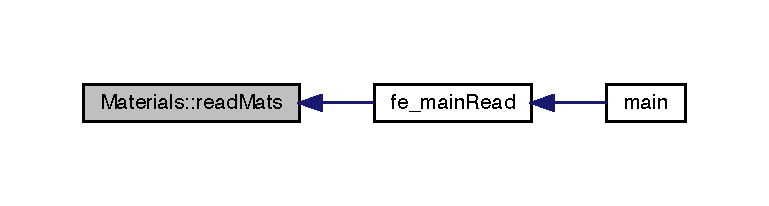
\includegraphics[width=350pt]{class_materials_a06e59a5742730b2292d39b7488523505_icgraph}
\end{center}
\end{figure}


\subsection{Friends And Related Function Documentation}
\mbox{\Hypertarget{class_materials_af7ffbad6dfcc99fc88b130c1a7b1720a}\label{class_materials_af7ffbad6dfcc99fc88b130c1a7b1720a}} 
\index{Materials@{Materials}!fe\+\_\+get\+\_\+mats@{fe\+\_\+get\+\_\+mats}}
\index{fe\+\_\+get\+\_\+mats@{fe\+\_\+get\+\_\+mats}!Materials@{Materials}}
\subsubsection{\texorpdfstring{fe\+\_\+get\+\_\+mats}{fe\_get\_mats}}
{\footnotesize\ttfamily double fe\+\_\+get\+\_\+mats (\begin{DoxyParamCaption}\item[{int}]{matl\+\_\+code,  }\item[{int}]{obj\+\_\+interest }\end{DoxyParamCaption})\hspace{0.3cm}{\ttfamily [friend]}}

Extracts the material parameter values based on the material id 

Definition at line 5 of file fe\+\_\+get\+\_\+mats.\+cpp.

\mbox{\Hypertarget{class_materials_a34d6fb85943d945b7e8600d2ef4220d0}\label{class_materials_a34d6fb85943d945b7e8600d2ef4220d0}} 
\index{Materials@{Materials}!fe\+\_\+get\+\_\+model@{fe\+\_\+get\+\_\+model}}
\index{fe\+\_\+get\+\_\+model@{fe\+\_\+get\+\_\+model}!Materials@{Materials}}
\subsubsection{\texorpdfstring{fe\+\_\+get\+\_\+model}{fe\_get\_model}}
{\footnotesize\ttfamily std\+::string fe\+\_\+get\+\_\+model (\begin{DoxyParamCaption}\item[{int}]{matl\+\_\+code }\end{DoxyParamCaption})\hspace{0.3cm}{\ttfamily [friend]}}



Definition at line 22 of file fe\+\_\+get\+\_\+mats.\+cpp.

\mbox{\Hypertarget{class_materials_ae66f6b31b5ad750f1fe042a706a4e3d4}\label{class_materials_ae66f6b31b5ad750f1fe042a706a4e3d4}} 
\index{Materials@{Materials}!main@{main}}
\index{main@{main}!Materials@{Materials}}
\subsubsection{\texorpdfstring{main}{main}}
{\footnotesize\ttfamily int main (\begin{DoxyParamCaption}{ }\end{DoxyParamCaption})\hspace{0.3cm}{\ttfamily [friend]}}

This is the main file. If you want to submit a new job -- this is where you do it Constants used in the code

Enter the path address for your job folder

What is the Problem Dimension -\/ Degrees of Freedom per node?

Simulation start time

Simulation end time

Output frequency -- result ouputs for every 100 timesteps

Maximum time step

Reduction factor

Type of Loading 1 -\/ Force based 2 -\/ Displacement based

Loading Amplitude

number of nodes $\ast$ number of directions

Degrees of freedom index data

Number of boundary condition constraints

Which nodes are constrained ?

index corresponding to the constrained degrees of freedom

Displacements of the constrained degrees of freedom

Enter your choice for type of simulations below, based on the following options\+: 1 -\/ Explicit Dynamic 2 -\/ Implicit Dynamic 3 -\/ Static Analysis

Definition at line 119 of file main.\+cpp.



The documentation for this class was generated from the following files\+:\begin{DoxyCompactItemize}
\item 
headers/\hyperlink{_materials_8h}{Materials.\+h}\item 
source/\+Input-\/\+Output/\+Input/\hyperlink{_materials_8cpp}{Materials.\+cpp}\end{DoxyCompactItemize}

\hypertarget{class_mesh}{}\section{Mesh Class Reference}
\label{class_mesh}\index{Mesh@{Mesh}}


{\ttfamily \#include $<$Mesh.\+h$>$}

\subsection*{Public Member Functions}
\begin{DoxyCompactItemize}
\item 
void \hyperlink{class_mesh_a2e0931c78a7ef01ccc9bf8f0dd74afb0}{read\+Mesh} (Matrix\+Xd n, Matrix\+Xd e)
\item 
Matrix\+Xd \hyperlink{class_mesh_a0b0f7458f07745240d9bda967cda12de}{get\+Nodes} ()
\item 
Matrix\+Xd \hyperlink{class_mesh_af3cbe568c8a36832659ac01025e8d774}{get\+Elements} ()
\item 
Matrix\+Xd \hyperlink{class_mesh_a52ecce406bbef80cbf3610db3ea5ea40}{get\+New\+Nodes} ()
\item 
Matrix\+Xd \hyperlink{class_mesh_af242dbb4627c09410975a0e67389e0de}{get\+New\+Elements} ()
\item 
void \hyperlink{class_mesh_aa8a6f260e9589be4c0a2fcc146e696d5}{preprocess\+Mesh} ()
\end{DoxyCompactItemize}


\subsection{Detailed Description}


Definition at line 23 of file Mesh.\+h.



\subsection{Member Function Documentation}
\mbox{\Hypertarget{class_mesh_af3cbe568c8a36832659ac01025e8d774}\label{class_mesh_af3cbe568c8a36832659ac01025e8d774}} 
\index{Mesh@{Mesh}!get\+Elements@{get\+Elements}}
\index{get\+Elements@{get\+Elements}!Mesh@{Mesh}}
\subsubsection{\texorpdfstring{get\+Elements()}{getElements()}}
{\footnotesize\ttfamily Matrix\+Xd Mesh\+::get\+Elements (\begin{DoxyParamCaption}\item[{void}]{ }\end{DoxyParamCaption})}



Definition at line 15 of file Mesh.\+cpp.

\mbox{\Hypertarget{class_mesh_af242dbb4627c09410975a0e67389e0de}\label{class_mesh_af242dbb4627c09410975a0e67389e0de}} 
\index{Mesh@{Mesh}!get\+New\+Elements@{get\+New\+Elements}}
\index{get\+New\+Elements@{get\+New\+Elements}!Mesh@{Mesh}}
\subsubsection{\texorpdfstring{get\+New\+Elements()}{getNewElements()}}
{\footnotesize\ttfamily Matrix\+Xd Mesh\+::get\+New\+Elements (\begin{DoxyParamCaption}\item[{void}]{ }\end{DoxyParamCaption})}



Definition at line 23 of file Mesh.\+cpp.

Here is the caller graph for this function\+:
\nopagebreak
\begin{figure}[H]
\begin{center}
\leavevmode
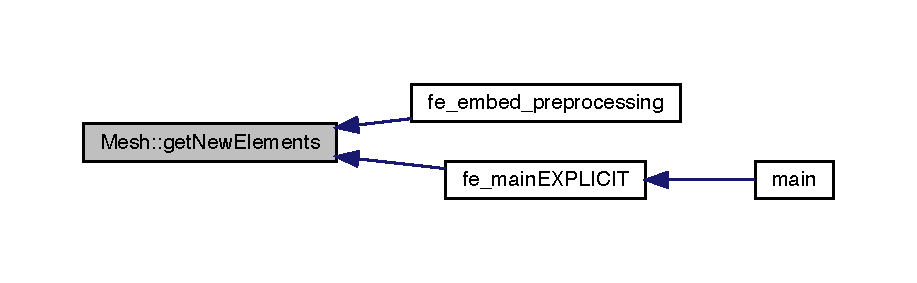
\includegraphics[width=350pt]{class_mesh_af242dbb4627c09410975a0e67389e0de_icgraph}
\end{center}
\end{figure}
\mbox{\Hypertarget{class_mesh_a52ecce406bbef80cbf3610db3ea5ea40}\label{class_mesh_a52ecce406bbef80cbf3610db3ea5ea40}} 
\index{Mesh@{Mesh}!get\+New\+Nodes@{get\+New\+Nodes}}
\index{get\+New\+Nodes@{get\+New\+Nodes}!Mesh@{Mesh}}
\subsubsection{\texorpdfstring{get\+New\+Nodes()}{getNewNodes()}}
{\footnotesize\ttfamily Matrix\+Xd Mesh\+::get\+New\+Nodes (\begin{DoxyParamCaption}\item[{void}]{ }\end{DoxyParamCaption})}



Definition at line 19 of file Mesh.\+cpp.

Here is the caller graph for this function\+:
\nopagebreak
\begin{figure}[H]
\begin{center}
\leavevmode
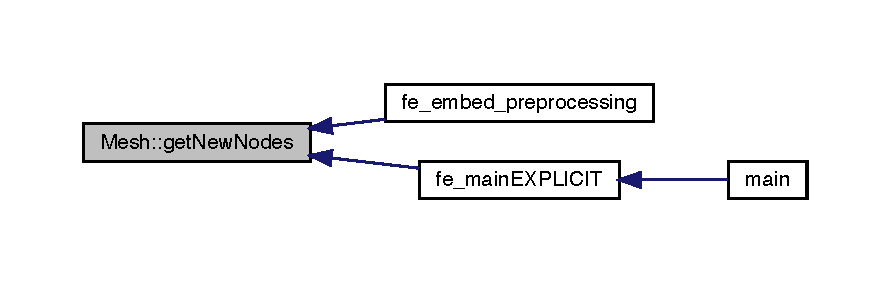
\includegraphics[width=350pt]{class_mesh_a52ecce406bbef80cbf3610db3ea5ea40_icgraph}
\end{center}
\end{figure}
\mbox{\Hypertarget{class_mesh_a0b0f7458f07745240d9bda967cda12de}\label{class_mesh_a0b0f7458f07745240d9bda967cda12de}} 
\index{Mesh@{Mesh}!get\+Nodes@{get\+Nodes}}
\index{get\+Nodes@{get\+Nodes}!Mesh@{Mesh}}
\subsubsection{\texorpdfstring{get\+Nodes()}{getNodes()}}
{\footnotesize\ttfamily Matrix\+Xd Mesh\+::get\+Nodes (\begin{DoxyParamCaption}\item[{void}]{ }\end{DoxyParamCaption})}



Definition at line 11 of file Mesh.\+cpp.

\mbox{\Hypertarget{class_mesh_aa8a6f260e9589be4c0a2fcc146e696d5}\label{class_mesh_aa8a6f260e9589be4c0a2fcc146e696d5}} 
\index{Mesh@{Mesh}!preprocess\+Mesh@{preprocess\+Mesh}}
\index{preprocess\+Mesh@{preprocess\+Mesh}!Mesh@{Mesh}}
\subsubsection{\texorpdfstring{preprocess\+Mesh()}{preprocessMesh()}}
{\footnotesize\ttfamily void Mesh\+::preprocess\+Mesh (\begin{DoxyParamCaption}\item[{void}]{ }\end{DoxyParamCaption})}

Nodes Preprocessing -\/ Putting the numbering in order

Elements Preprocessing -\/ Correcting the element definitions

find\+\_\+in\+\_\+matrix gives the row number of node in nodes matrix 

Definition at line 27 of file Mesh.\+cpp.

Here is the call graph for this function\+:
\nopagebreak
\begin{figure}[H]
\begin{center}
\leavevmode
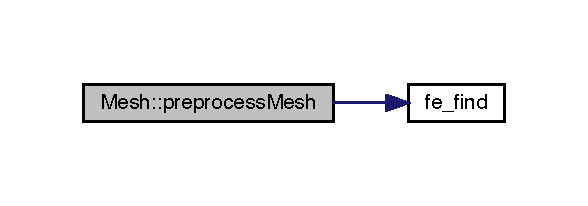
\includegraphics[width=282pt]{class_mesh_aa8a6f260e9589be4c0a2fcc146e696d5_cgraph}
\end{center}
\end{figure}
Here is the caller graph for this function\+:
\nopagebreak
\begin{figure}[H]
\begin{center}
\leavevmode
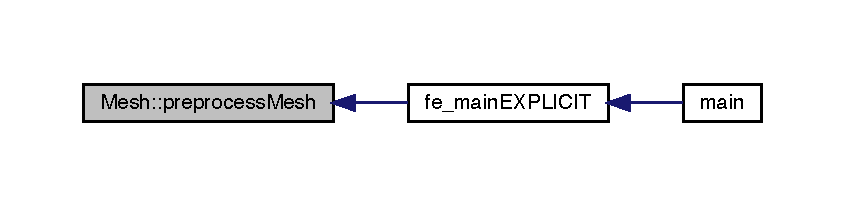
\includegraphics[width=350pt]{class_mesh_aa8a6f260e9589be4c0a2fcc146e696d5_icgraph}
\end{center}
\end{figure}
\mbox{\Hypertarget{class_mesh_a2e0931c78a7ef01ccc9bf8f0dd74afb0}\label{class_mesh_a2e0931c78a7ef01ccc9bf8f0dd74afb0}} 
\index{Mesh@{Mesh}!read\+Mesh@{read\+Mesh}}
\index{read\+Mesh@{read\+Mesh}!Mesh@{Mesh}}
\subsubsection{\texorpdfstring{read\+Mesh()}{readMesh()}}
{\footnotesize\ttfamily void Mesh\+::read\+Mesh (\begin{DoxyParamCaption}\item[{Matrix\+Xd}]{n,  }\item[{Matrix\+Xd}]{e }\end{DoxyParamCaption})}



Definition at line 6 of file Mesh.\+cpp.

Here is the caller graph for this function\+:
\nopagebreak
\begin{figure}[H]
\begin{center}
\leavevmode
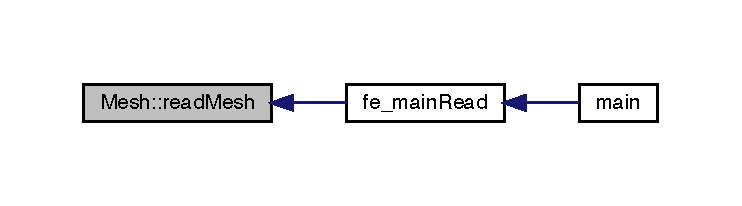
\includegraphics[width=350pt]{class_mesh_a2e0931c78a7ef01ccc9bf8f0dd74afb0_icgraph}
\end{center}
\end{figure}


The documentation for this class was generated from the following files\+:\begin{DoxyCompactItemize}
\item 
headers/\hyperlink{_mesh_8h}{Mesh.\+h}\item 
source/\+Input-\/\+Output/\+Input/\hyperlink{_mesh_8cpp}{Mesh.\+cpp}\end{DoxyCompactItemize}

\chapter{File Documentation}
\hypertarget{input_8inp}{}\section{examples/example-\/1/input.inp File Reference}
\label{input_8inp}\index{examples/example-\/1/input.\+inp@{examples/example-\/1/input.\+inp}}

\hypertarget{functions_8h}{}\section{/\+Users/vsg111/\+Dropbox/\+Work/\+Papers/\+Paper\+\_\+\+E\+E\+M\+\_\+\+Computational/\+E\+E\+M\+\_\+\+Dynamic/headers/functions.h File Reference}
\label{functions_8h}\index{/\+Users/vsg111/\+Dropbox/\+Work/\+Papers/\+Paper\+\_\+\+E\+E\+M\+\_\+\+Computational/\+E\+E\+M\+\_\+\+Dynamic/headers/functions.\+h@{/\+Users/vsg111/\+Dropbox/\+Work/\+Papers/\+Paper\+\_\+\+E\+E\+M\+\_\+\+Computational/\+E\+E\+M\+\_\+\+Dynamic/headers/functions.\+h}}
{\ttfamily \#include $<$iostream$>$}\newline
{\ttfamily \#include $<$cmath$>$}\newline
{\ttfamily \#include $<$vector$>$}\newline
{\ttfamily \#include $<$fstream$>$}\newline
{\ttfamily \#include $<$sstream$>$}\newline
{\ttfamily \#include $<$string$>$}\newline
{\ttfamily \#include $<$iomanip$>$}\newline
{\ttfamily \#include \char`\"{}Eigen/\+Dense\char`\"{}}\newline
{\ttfamily \#include \char`\"{}Eigen/\+Eigenvalues\char`\"{}}\newline
{\ttfamily \#include \char`\"{}unsupported/\+Eigen/\+Matrix\+Functions\char`\"{}}\newline
{\ttfamily \#include \char`\"{}Mesh.\+h\char`\"{}}\newline
{\ttfamily \#include \char`\"{}Materials.\+h\char`\"{}}\newline
\subsection*{Functions}
\begin{DoxyCompactItemize}
\item 
Matrix\+Xd \hyperlink{functions_8h_add4fca63e194477644c3388febf88023}{text2matrix} (std\+::string name, int cols)
\item 
Vector\+Xd \hyperlink{functions_8h_ab77a3a6d6f6b436d7e8c600bb0869927}{fe\+\_\+shapes\+\_\+8} (double rvalue, double svalue, double tvalue)
\item 
Vector\+Xd \hyperlink{functions_8h_afc547bef246c057db6cbd04bf7f866a9}{fe\+\_\+dndr\+\_\+8} (double rvalue, double svalue, double tvalue)
\item 
Vector\+Xd \hyperlink{functions_8h_ac0b5524525e1f2e89bb064c15ab8e664}{fe\+\_\+dnds\+\_\+8} (double rvalue, double svalue, double tvalue)
\item 
Vector\+Xd \hyperlink{functions_8h_a57e8e5c9f740c98e4767f29c121c2d0a}{fe\+\_\+dndt\+\_\+8} (double rvalue, double svalue, double tvalue)
\item 
Vector\+Xd \hyperlink{functions_8h_aa6ab8c3298fa10734e299fe8266aed35}{guass\+\_\+points} (int n)
\item 
Vector\+Xd \hyperlink{functions_8h_a84dcc9575e861bdb2872c10ba6238ee4}{guass\+\_\+weights} (int n)
\item 
Matrix\+Xd \hyperlink{functions_8h_a502e3469e1cc253deb142f46c0789a78}{guass\+\_\+points\+\_\+3d} (int nx, int ny, int nz)
\item 
Matrix\+Xd \hyperlink{functions_8h_ad99b08ce65ae353e91486d7685c22024}{guass\+\_\+weights\+\_\+3d} (int \hyperlink{main_8cpp_aa789fe4d8a13fd0990b630909430d5d0}{ndof}, int nx, int ny, int nz)
\item 
Matrix\+Xd \hyperlink{functions_8h_ada816506319851dcff162fa5e54d72d5}{fe\+\_\+iso\+Elastic} (int n, double E, double nu)
\item 
Matrix\+Xd \hyperlink{functions_8h_a12aa5a7a3443c6fcc5e65d3bcfc9bcc3}{fe\+\_\+cal\+Jacobian} (int dim, int nnel, Vector\+Xd dndr, Vector\+Xd dnds, Vector\+Xd dndt, double xcoord\mbox{[}$\,$\mbox{]}, double ycoord\mbox{[}$\,$\mbox{]}, double zcoord\mbox{[}$\,$\mbox{]})
\item 
Vector\+Xd \hyperlink{functions_8h_afc6be1a5667e68156cb099e8da71170f}{fe\+\_\+dndx\+\_\+8} (int nnel, Vector\+Xd dndr, Vector\+Xd dnds, Vector\+Xd dndt, Matrix\+Xd inv\+Jacobian)
\item 
Vector\+Xd \hyperlink{functions_8h_a0572d7818e085c67f7fbb84eef8ecfb4}{fe\+\_\+dndy\+\_\+8} (int nnel, Vector\+Xd dndr, Vector\+Xd dnds, Vector\+Xd dndt, Matrix\+Xd inv\+Jacobian)
\item 
Vector\+Xd \hyperlink{functions_8h_aaf75db8433433807839c6ea17f2cf72c}{fe\+\_\+dndz\+\_\+8} (int nnel, Vector\+Xd dndr, Vector\+Xd dnds, Vector\+Xd dndt, Matrix\+Xd inv\+Jacobian)
\item 
Matrix\+Xd \hyperlink{functions_8h_a4b49d2df4f86e7d0755971ab4bfa48b2}{fe\+\_\+str\+Disp\+Matrix} (int edof, int nnel, Vector\+Xd dndx, Vector\+Xd dndy, Vector\+Xd dndz)
\item 
Matrix\+Xd \hyperlink{functions_8h_a3c73fda948017ac96aeb19889cfc1cba}{fe\+\_\+apply\+\_\+bc\+\_\+stiffness} (Matrix\+Xd kk, Vector\+Xi \hyperlink{main_8cpp_a389e085bd7632077f619ea67d3fb4087}{bcdof}, Vector\+Xd \hyperlink{main_8cpp_a3a53182d9f97dc5acff0a10125857cfb}{bcval})
\item 
Vector\+Xd \hyperlink{functions_8h_ac52c0e94b3bad1ca823301ad609a1549}{fe\+\_\+apply\+\_\+bc\+\_\+force} (Vector\+Xd ff, Vector\+Xi \hyperlink{main_8cpp_a389e085bd7632077f619ea67d3fb4087}{bcdof}, Vector\+Xd \hyperlink{main_8cpp_a3a53182d9f97dc5acff0a10125857cfb}{bcval})
\item 
void \hyperlink{functions_8h_a346547477d2a1fbeff6b5e0b05314283}{matrix2text} (std\+::string name, Matrix\+Xd new\+\_\+slave\+\_\+master, int width)
\item 
void \hyperlink{functions_8h_a0b5f62139051473c809da12cc0c45e29}{vector2text} (std\+::string name, Vector\+Xd vector, int width)
\item 
Matrix\+Xd \hyperlink{functions_8h_aa41c40dffea4251a07a8a3f5062f47ae}{fe\+\_\+cal\+Transformation} (Matrix\+Xd truss\+\_\+nodes, int choice)
\item 
Matrix\+Xd \hyperlink{functions_8h_ae2eeba997bf4f0bc4749b92130de7ba3}{fe\+\_\+cal\+Simp\+Transformation} (Matrix\+Xd truss\+\_\+nodes)
\item 
Matrix\+Xd \hyperlink{functions_8h_a9378d4fc517465015411134456235a76}{fe\+\_\+stiffness\+\_\+hex} (double E, double nu, int \hyperlink{main_8cpp_aa789fe4d8a13fd0990b630909430d5d0}{ndof}, int nnel, int edof, double xcoord\mbox{[}$\,$\mbox{]}, double ycoord\mbox{[}$\,$\mbox{]}, double zcoord\mbox{[}$\,$\mbox{]})
\item 
Matrix\+Xd \hyperlink{functions_8h_ab3798340a27f0972299b3820aab0ccba}{fe\+\_\+stiffness\+\_\+embed\+\_\+truss} (Matrix\+Xd nodes\+\_\+truss, Matrix\+Xd elements\+\_\+truss, double E\+\_\+truss, double \hyperlink{main_8cpp_a2f98cf28208251affb988effe3a89708}{A\+\_\+truss}, int \hyperlink{main_8cpp_aa789fe4d8a13fd0990b630909430d5d0}{ndof}, int nnel, int edof, double xcoord\mbox{[}$\,$\mbox{]}, double ycoord\mbox{[}$\,$\mbox{]}, double zcoord\mbox{[}$\,$\mbox{]})
\item 
Matrix\+Xd \hyperlink{functions_8h_a98fae74dde5fe33a7062e7457a2d3227}{fe\+\_\+shape\+Matrix} (int edof, int nnel, Vector\+Xd shapes)
\item 
Matrix\+Xd \hyperlink{functions_8h_a04906e61b8cfdc7232924a594b95eb1f}{fe\+\_\+mass\+\_\+hex} (double rho, int \hyperlink{main_8cpp_aa789fe4d8a13fd0990b630909430d5d0}{ndof}, int nnel, int edof, double xcoord\mbox{[}$\,$\mbox{]}, double ycoord\mbox{[}$\,$\mbox{]}, double zcoord\mbox{[}$\,$\mbox{]})
\item 
Vector\+Xd \hyperlink{functions_8h_a7d0fd8cfef8b891901eb6f0f780fd9f2}{fe\+\_\+stress\+Update} (Vector\+Xd dndx, Vector\+Xd dndy, Vector\+Xd dndz, Matrix\+Xd disp\+\_\+mat, Vector\+Xd u, int opt, int return\+\_\+opt)
\item 
Vector\+Xd \hyperlink{functions_8h_aa8f7f6d72c6b57c721b23a38e2e20fc5}{fe\+\_\+getforce} (Matrix\+Xd nodes, Matrix\+Xd elements, int \hyperlink{main_8cpp_aa789fe4d8a13fd0990b630909430d5d0}{ndof}, Vector\+Xd u, Vector\+Xd v, Vector\+Xd fext, int size\+\_\+counter, Matrix\+Xd nodes\+\_\+truss, Matrix\+Xd elements\+\_\+truss)
\begin{DoxyCompactList}\small\item\em Calculates the resultant nodal force after each time step. \end{DoxyCompactList}\item 
double \hyperlink{functions_8h_af737926a3dfd669254a56dbbf675ac92}{fe\+\_\+get\+Time\+Step} (Matrix\+Xd nodes, Matrix\+Xd elements, int \hyperlink{main_8cpp_aa789fe4d8a13fd0990b630909430d5d0}{ndof}, Vector\+Xd u, Vector\+Xd v, Vector\+Xd fext)
\item 
double \hyperlink{functions_8h_ab0d9d059d2b8f829000e6f1f7d1d4ffb}{fe\+\_\+cal\+Time\+Step} (double xcoord\mbox{[}$\,$\mbox{]}, double ycoord\mbox{[}$\,$\mbox{]}, double zcoord\mbox{[}$\,$\mbox{]}, double E, double nu, double rho)
\item 
double \hyperlink{functions_8h_ac1306a43db522f3da30471d2a6c48686}{fe\+\_\+cal\+Area\+\_\+4} (double a1, double a2, double a3, double a4, double b1, double b2, double b3, double b4, double c1, double c2, double c3, double c4)
\item 
double \hyperlink{functions_8h_afbe30e3a940236fc486b96028abf6f46}{fe\+\_\+cal\+Volume} (double xcoord\mbox{[}$\,$\mbox{]}, double ycoord\mbox{[}$\,$\mbox{]}, double zcoord\mbox{[}$\,$\mbox{]})
\item 
Vector\+Xd \hyperlink{functions_8h_a42274df47bb3a633055b1ccbb2f920ae}{fe\+\_\+apply\+\_\+bc\+\_\+displacement} (Vector\+Xd U, Vector\+Xi \hyperlink{main_8cpp_a389e085bd7632077f619ea67d3fb4087}{bcdof}, Vector\+Xd \hyperlink{main_8cpp_a3a53182d9f97dc5acff0a10125857cfb}{bcval})
\item 
void \hyperlink{functions_8h_ab3e39c6d01b6fd10c9e264731cef75dc}{fe\+\_\+display\+\_\+vector} (Vector\+Xd A)
\item 
void \hyperlink{functions_8h_a5110a192d089c6b26744b9e9d67a7c2d}{fe\+\_\+display\+\_\+matrix} (Matrix\+Xd A)
\item 
Matrix\+Xd \hyperlink{functions_8h_ab747d046148af042245ed13ca720c5ec}{fe\+\_\+transform\+Mass} (Matrix\+Xd m, int opt)
\item 
double \hyperlink{functions_8h_af7ffbad6dfcc99fc88b130c1a7b1720a}{fe\+\_\+get\+\_\+mats} (int matl\+\_\+code, int obj\+\_\+interest)
\item 
std\+::string \hyperlink{functions_8h_a34d6fb85943d945b7e8600d2ef4220d0}{fe\+\_\+get\+\_\+model} (int matl\+\_\+code)
\item 
Matrix\+Xd \hyperlink{functions_8h_a8c9fd519c93c847cdf52de947964eb67}{fe\+\_\+str\+Disp\+Matrix\+\_\+total\+Lagrangian} (int edof, int nnel, Vector\+Xd dndx, Vector\+Xd dndy, Vector\+Xd dndz, Vector\+Xd u)
\item 
Matrix\+Xd \hyperlink{functions_8h_ae50379f74802347e04dbc022897f9cb0}{fe\+\_\+cal\+Def\+Grad} (Vector\+Xd dndx, Vector\+Xd dndy, Vector\+Xd dndz, Vector\+Xd u)
\item 
double \hyperlink{functions_8h_acb1ae85901899b3e4e2a1635e036fd35}{fe\+\_\+cal\+Wave\+Speed} (double E, double nu, double rho)
\item 
void \hyperlink{functions_8h_a9dec90c41460e15aa1d8dce787683406}{fe\+\_\+write\+Element\+Stress} (Matrix\+Xd sigma\+\_\+all, double time)
\item 
Matrix\+Xd \hyperlink{functions_8h_a350d27ea0f1de929495d659b26f428d2}{fe\+\_\+mass\+\_\+truss} (double rho, double \hyperlink{main_8cpp_a2f98cf28208251affb988effe3a89708}{A\+\_\+truss}, int edof, Matrix\+Xd nodes, Matrix\+Xd elements)
\item 
Vector\+Xd \hyperlink{functions_8h_a94c1b672863e28bc2c70d08726939929}{fe\+\_\+stress\+Update\+\_\+1d} (Vector\+Xd dndx, Vector\+Xd dndy, Vector\+Xd dndz, Vector\+Xd u\+\_\+e, int opt, Matrix\+Xd nodes)
\item 
void \hyperlink{functions_8h_a45a1daa8de18fc5fc463f9b569970245}{fe\+\_\+vtk\+Write\+\_\+host} (std\+::string output, int format\+\_\+choice, int mesh\+\_\+choice, int time\+\_\+step, Matrix\+Xd nodes, Matrix\+Xd elements)
\item 
void \hyperlink{functions_8h_a6e838460f501267efe34f29d4cf6d9cd}{fe\+\_\+vtk\+Write\+\_\+truss} (std\+::string output, int format\+\_\+choice, int mesh\+\_\+choice, int time\+\_\+step, Matrix\+Xd nodes, Matrix\+Xd elements)
\item 
Matrix\+Xd \hyperlink{functions_8h_a81ce693c4400df82b8753f25cc2dcabc}{fe\+\_\+update\+Nodes} (Matrix\+Xd nodes, Vector\+Xd displacements)
\item 
void \hyperlink{functions_8h_ab2f8704631ca6c23a453d1905efbb162}{fe\+\_\+main\+E\+X\+P\+L\+I\+C\+IT} ()
\begin{DoxyCompactList}\small\item\em This function carries out the explicit dynamic analysis of the F\+EM problem. \end{DoxyCompactList}\item 
Vector\+Xi \hyperlink{functions_8h_ae4dbe24b761cafa3577afab76726b382}{fe\+\_\+find\+\_\+index} (Vector\+Xi node\+\_\+list)
\item 
Matrix\+Xd \hyperlink{functions_8h_a04f569c566ca4fbea3b3a2a13cdd0af5}{fe\+\_\+assemble\+\_\+mass} (Matrix\+Xd mm, Matrix\+Xd m, Vector\+Xi node\+\_\+list, int sdof)
\item 
Vector\+Xd \hyperlink{functions_8h_ab5053cb12ac67971a7836346e2839725}{fe\+\_\+gather} (Vector\+Xd global\+\_\+vec, Vector\+Xd local\+\_\+vec, Vector\+Xi node\+\_\+list, int sdof)
\item 
Vector\+Xd \hyperlink{functions_8h_a6b8344e12f9005795f93f60ddda26c5c}{fe\+\_\+scatter} (Vector\+Xd global\+\_\+vec, Vector\+Xd local\+\_\+vec, Vector\+Xi node\+\_\+list, int sdof)
\item 
Vector\+Xd \hyperlink{functions_8h_a73c4523ec7068af2af9e8431021f5fdf}{fe\+\_\+tensor2voigt} (Matrix\+Xd A)
\item 
Matrix\+Xd \hyperlink{functions_8h_a721a169d6a3d34b5584817ccd1c48cd7}{fe\+\_\+voigt2tensor} (Vector\+Xd B)
\item 
Matrix\+Xd \hyperlink{functions_8h_ac2d90cb6719488bc8551e6f9437f4f76}{fe\+\_\+concatenate\+\_\+vector2matrix} (Matrix\+Xd A, Vector\+Xd B, int opt)
\item 
int \hyperlink{functions_8h_a983304137f9a961469a558437d5d2d59}{fe\+\_\+find} (Vector\+Xd A, double a)
\item 
void \hyperlink{functions_8h_a8a64e915e17f876fe72bedd820e87c33}{fe\+\_\+main\+Read} (std\+::string file)
\end{DoxyCompactItemize}
\subsection*{Variables}
\begin{DoxyCompactItemize}
\item 
std\+::string \hyperlink{functions_8h_a556ce46e457f991c51f3dac111579e2b}{home\+\_\+path}
\item 
std\+::string \hyperlink{functions_8h_a5e3d7c3d50f127de0e61daaa407dc7d1}{job\+\_\+file}
\item 
int \hyperlink{functions_8h_aa789fe4d8a13fd0990b630909430d5d0}{ndof}
\item 
int \hyperlink{functions_8h_a509bc84434af1eff0173e4a71bd758ac}{num\+\_\+meshes}
\item 
\hyperlink{class_mesh}{Mesh} $\ast$ \hyperlink{functions_8h_a6e08f89b32254fb4b129720418e7c6ea}{mesh}
\item 
double \hyperlink{functions_8h_a1b01a4354147da92a548ea1a5f96d592}{t\+\_\+start}
\item 
double \hyperlink{functions_8h_a4b637c5fff609e604a3b2b2787f4a9fa}{t\+\_\+end}
\item 
int \hyperlink{functions_8h_ace6ace9b2f6d8d404ca9e66564289eb1}{output\+\_\+frequency}
\item 
double \hyperlink{functions_8h_a068c627ac33cf3c721d8f28eab205a83}{dt\+\_\+initial}
\item 
double \hyperlink{functions_8h_a0a612324885914b6799185d54c48b310}{dt\+\_\+min}
\item 
double \hyperlink{functions_8h_a7700f3aeb1ca1c9bbbf712dbfb0aa349}{reduction}
\item 
int \hyperlink{functions_8h_a39328cf72d69139b3b6c5b8ef6c636fe}{material\+\_\+types}
\item 
\hyperlink{class_materials}{Materials} $\ast$ \hyperlink{functions_8h_acfa6799b35f9301b5fc44e6043624797}{mat}
\item 
double \hyperlink{functions_8h_a41b0f465c44fe8b2de43cfaa05bb7880}{input\+\_\+load\+\_\+amp}
\item 
Vector\+Xi \hyperlink{functions_8h_ab49fb3bb15f9624e4ffb12a75c7db55d}{fcdof}
\item 
Vector\+Xd \hyperlink{functions_8h_ac1f3d4744efb6ce0d6c5b89774ba91aa}{fcload}
\item 
int \hyperlink{functions_8h_abd406f244d4145ae5baf4ea059b5232d}{num\+\_\+constraints}
\item 
Vector\+Xi \hyperlink{functions_8h_a389e085bd7632077f619ea67d3fb4087}{bcdof}
\item 
Vector\+Xd \hyperlink{functions_8h_a3a53182d9f97dc5acff0a10125857cfb}{bcval}
\item 
Matrix\+Xd \hyperlink{functions_8h_a6f626bfc805c8f0fb5170c06b4e61c8a}{element\+\_\+stress\+\_\+host}
\item 
Matrix\+Xd \hyperlink{functions_8h_a1db1555bea7ef22b3783cdd66ebbeb0e}{element\+\_\+strain\+\_\+host}
\item 
Matrix\+Xd \hyperlink{functions_8h_a1ae14dd64a0bd3139f1e153dc5e48016}{element\+\_\+stress\+\_\+truss}
\item 
Matrix\+Xd \hyperlink{functions_8h_a296db0b5edbd14e04e368f248587c4eb}{element\+\_\+strain\+\_\+truss}
\item 
Vector\+Xd \hyperlink{functions_8h_ae07dc1b145ffa9093a4262baf26aff7a}{fi\+\_\+prev}
\item 
Vector\+Xd \hyperlink{functions_8h_a7a1410ed488bb0dd5c10344c4c4951e6}{fi\+\_\+curr}
\item 
Vector\+Xd \hyperlink{functions_8h_a3ebb0eb4b098a0ac9e1f24de934a282f}{W\+\_\+int}
\item 
Vector\+Xd \hyperlink{functions_8h_a032d9f703d3d55ca1e54f14f44457615}{U\+\_\+host}
\item 
Vector\+Xd \hyperlink{functions_8h_ad72fa62a83a5fde880ab78c8c81c48bb}{V\+\_\+host}
\item 
Vector\+Xd \hyperlink{functions_8h_a7a1e6ce58aaa0309efd50328e8f295e9}{A\+\_\+host}
\item 
Vector\+Xd \hyperlink{functions_8h_a94430566d55ccfa65e497716fd404dea}{U\+\_\+truss}
\item 
Vector\+Xd \hyperlink{functions_8h_a5159843113dbbfc6e912c3345c0a7916}{V\+\_\+truss}
\item 
Vector\+Xd \hyperlink{functions_8h_a2f98cf28208251affb988effe3a89708}{A\+\_\+truss}
\end{DoxyCompactItemize}


\subsection{Function Documentation}
\mbox{\Hypertarget{functions_8h_a42274df47bb3a633055b1ccbb2f920ae}\label{functions_8h_a42274df47bb3a633055b1ccbb2f920ae}} 
\index{functions.\+h@{functions.\+h}!fe\+\_\+apply\+\_\+bc\+\_\+displacement@{fe\+\_\+apply\+\_\+bc\+\_\+displacement}}
\index{fe\+\_\+apply\+\_\+bc\+\_\+displacement@{fe\+\_\+apply\+\_\+bc\+\_\+displacement}!functions.\+h@{functions.\+h}}
\subsubsection{\texorpdfstring{fe\+\_\+apply\+\_\+bc\+\_\+displacement()}{fe\_apply\_bc\_displacement()}}
{\footnotesize\ttfamily Vector\+Xd fe\+\_\+apply\+\_\+bc\+\_\+displacement (\begin{DoxyParamCaption}\item[{Vector\+Xd}]{U,  }\item[{Vector\+Xi}]{bcdof,  }\item[{Vector\+Xd}]{bcval }\end{DoxyParamCaption})}



Definition at line 5 of file fe\+\_\+apply\+\_\+bc.\+cpp.

\mbox{\Hypertarget{functions_8h_ac52c0e94b3bad1ca823301ad609a1549}\label{functions_8h_ac52c0e94b3bad1ca823301ad609a1549}} 
\index{functions.\+h@{functions.\+h}!fe\+\_\+apply\+\_\+bc\+\_\+force@{fe\+\_\+apply\+\_\+bc\+\_\+force}}
\index{fe\+\_\+apply\+\_\+bc\+\_\+force@{fe\+\_\+apply\+\_\+bc\+\_\+force}!functions.\+h@{functions.\+h}}
\subsubsection{\texorpdfstring{fe\+\_\+apply\+\_\+bc\+\_\+force()}{fe\_apply\_bc\_force()}}
{\footnotesize\ttfamily Vector\+Xd fe\+\_\+apply\+\_\+bc\+\_\+force (\begin{DoxyParamCaption}\item[{Vector\+Xd}]{ff,  }\item[{Vector\+Xi}]{bcdof,  }\item[{Vector\+Xd}]{bcval }\end{DoxyParamCaption})}



Definition at line 17 of file fe\+\_\+apply\+\_\+bc.\+cpp.

\mbox{\Hypertarget{functions_8h_a3c73fda948017ac96aeb19889cfc1cba}\label{functions_8h_a3c73fda948017ac96aeb19889cfc1cba}} 
\index{functions.\+h@{functions.\+h}!fe\+\_\+apply\+\_\+bc\+\_\+stiffness@{fe\+\_\+apply\+\_\+bc\+\_\+stiffness}}
\index{fe\+\_\+apply\+\_\+bc\+\_\+stiffness@{fe\+\_\+apply\+\_\+bc\+\_\+stiffness}!functions.\+h@{functions.\+h}}
\subsubsection{\texorpdfstring{fe\+\_\+apply\+\_\+bc\+\_\+stiffness()}{fe\_apply\_bc\_stiffness()}}
{\footnotesize\ttfamily Matrix\+Xd fe\+\_\+apply\+\_\+bc\+\_\+stiffness (\begin{DoxyParamCaption}\item[{Matrix\+Xd}]{kk,  }\item[{Vector\+Xi}]{bcdof,  }\item[{Vector\+Xd}]{bcval }\end{DoxyParamCaption})}



Definition at line 29 of file fe\+\_\+apply\+\_\+bc.\+cpp.

\mbox{\Hypertarget{functions_8h_a04f569c566ca4fbea3b3a2a13cdd0af5}\label{functions_8h_a04f569c566ca4fbea3b3a2a13cdd0af5}} 
\index{functions.\+h@{functions.\+h}!fe\+\_\+assemble\+\_\+mass@{fe\+\_\+assemble\+\_\+mass}}
\index{fe\+\_\+assemble\+\_\+mass@{fe\+\_\+assemble\+\_\+mass}!functions.\+h@{functions.\+h}}
\subsubsection{\texorpdfstring{fe\+\_\+assemble\+\_\+mass()}{fe\_assemble\_mass()}}
{\footnotesize\ttfamily Matrix\+Xd fe\+\_\+assemble\+\_\+mass (\begin{DoxyParamCaption}\item[{Matrix\+Xd}]{mm,  }\item[{Matrix\+Xd}]{m,  }\item[{Vector\+Xi}]{node\+\_\+list,  }\item[{int}]{sdof }\end{DoxyParamCaption})}

Assembles the global mass matrix 

Definition at line 24 of file fe\+\_\+assemble\+\_\+mass.\+cpp.

\mbox{\Hypertarget{functions_8h_ac1306a43db522f3da30471d2a6c48686}\label{functions_8h_ac1306a43db522f3da30471d2a6c48686}} 
\index{functions.\+h@{functions.\+h}!fe\+\_\+cal\+Area\+\_\+4@{fe\+\_\+cal\+Area\+\_\+4}}
\index{fe\+\_\+cal\+Area\+\_\+4@{fe\+\_\+cal\+Area\+\_\+4}!functions.\+h@{functions.\+h}}
\subsubsection{\texorpdfstring{fe\+\_\+cal\+Area\+\_\+4()}{fe\_calArea\_4()}}
{\footnotesize\ttfamily double fe\+\_\+cal\+Area\+\_\+4 (\begin{DoxyParamCaption}\item[{double}]{a1,  }\item[{double}]{a2,  }\item[{double}]{a3,  }\item[{double}]{a4,  }\item[{double}]{b1,  }\item[{double}]{b2,  }\item[{double}]{b3,  }\item[{double}]{b4,  }\item[{double}]{c1,  }\item[{double}]{c2,  }\item[{double}]{c3,  }\item[{double}]{c4 }\end{DoxyParamCaption})}

Calculates the area of a face with 4 vertices 

Definition at line 5 of file fe\+\_\+cal\+Area\+\_\+4.\+cpp.

\mbox{\Hypertarget{functions_8h_ae50379f74802347e04dbc022897f9cb0}\label{functions_8h_ae50379f74802347e04dbc022897f9cb0}} 
\index{functions.\+h@{functions.\+h}!fe\+\_\+cal\+Def\+Grad@{fe\+\_\+cal\+Def\+Grad}}
\index{fe\+\_\+cal\+Def\+Grad@{fe\+\_\+cal\+Def\+Grad}!functions.\+h@{functions.\+h}}
\subsubsection{\texorpdfstring{fe\+\_\+cal\+Def\+Grad()}{fe\_calDefGrad()}}
{\footnotesize\ttfamily Matrix\+Xd fe\+\_\+cal\+Def\+Grad (\begin{DoxyParamCaption}\item[{Vector\+Xd}]{dndx,  }\item[{Vector\+Xd}]{dndy,  }\item[{Vector\+Xd}]{dndz,  }\item[{Vector\+Xd}]{u }\end{DoxyParamCaption})}

Calculates the deformation gradient 

Definition at line 7 of file fe\+\_\+cal\+Def\+Grad.\+cpp.

\mbox{\Hypertarget{functions_8h_a12aa5a7a3443c6fcc5e65d3bcfc9bcc3}\label{functions_8h_a12aa5a7a3443c6fcc5e65d3bcfc9bcc3}} 
\index{functions.\+h@{functions.\+h}!fe\+\_\+cal\+Jacobian@{fe\+\_\+cal\+Jacobian}}
\index{fe\+\_\+cal\+Jacobian@{fe\+\_\+cal\+Jacobian}!functions.\+h@{functions.\+h}}
\subsubsection{\texorpdfstring{fe\+\_\+cal\+Jacobian()}{fe\_calJacobian()}}
{\footnotesize\ttfamily Matrix\+Xd fe\+\_\+cal\+Jacobian (\begin{DoxyParamCaption}\item[{int}]{dim,  }\item[{int}]{nnel,  }\item[{Vector\+Xd}]{dndr,  }\item[{Vector\+Xd}]{dnds,  }\item[{Vector\+Xd}]{dndt,  }\item[{double}]{xcoord\mbox{[}$\,$\mbox{]},  }\item[{double}]{ycoord\mbox{[}$\,$\mbox{]},  }\item[{double}]{zcoord\mbox{[}$\,$\mbox{]} }\end{DoxyParamCaption})}

Calculates the jacobian -- using the derivates of shape functions 

Definition at line 7 of file fe\+\_\+cal\+Jacobian.\+cpp.

\mbox{\Hypertarget{functions_8h_ae2eeba997bf4f0bc4749b92130de7ba3}\label{functions_8h_ae2eeba997bf4f0bc4749b92130de7ba3}} 
\index{functions.\+h@{functions.\+h}!fe\+\_\+cal\+Simp\+Transformation@{fe\+\_\+cal\+Simp\+Transformation}}
\index{fe\+\_\+cal\+Simp\+Transformation@{fe\+\_\+cal\+Simp\+Transformation}!functions.\+h@{functions.\+h}}
\subsubsection{\texorpdfstring{fe\+\_\+cal\+Simp\+Transformation()}{fe\_calSimpTransformation()}}
{\footnotesize\ttfamily Matrix\+Xd fe\+\_\+cal\+Simp\+Transformation (\begin{DoxyParamCaption}\item[{Matrix\+Xd}]{truss\+\_\+nodes }\end{DoxyParamCaption})}



Definition at line 7 of file fe\+\_\+cal\+Simp\+Transformation.\+cpp.

\mbox{\Hypertarget{functions_8h_ab0d9d059d2b8f829000e6f1f7d1d4ffb}\label{functions_8h_ab0d9d059d2b8f829000e6f1f7d1d4ffb}} 
\index{functions.\+h@{functions.\+h}!fe\+\_\+cal\+Time\+Step@{fe\+\_\+cal\+Time\+Step}}
\index{fe\+\_\+cal\+Time\+Step@{fe\+\_\+cal\+Time\+Step}!functions.\+h@{functions.\+h}}
\subsubsection{\texorpdfstring{fe\+\_\+cal\+Time\+Step()}{fe\_calTimeStep()}}
{\footnotesize\ttfamily double fe\+\_\+cal\+Time\+Step (\begin{DoxyParamCaption}\item[{double}]{xcoord\mbox{[}$\,$\mbox{]},  }\item[{double}]{ycoord\mbox{[}$\,$\mbox{]},  }\item[{double}]{zcoord\mbox{[}$\,$\mbox{]},  }\item[{double}]{E,  }\item[{double}]{nu,  }\item[{double}]{rho }\end{DoxyParamCaption})}

Calculates the time step for a single element based on its dimensions and material model

For a single element -\/ this function calculates the volume of the element and calculates the critical time step based on the wave speed. 

Definition at line 5 of file fe\+\_\+cal\+Time\+Step.\+cpp.

\mbox{\Hypertarget{functions_8h_aa41c40dffea4251a07a8a3f5062f47ae}\label{functions_8h_aa41c40dffea4251a07a8a3f5062f47ae}} 
\index{functions.\+h@{functions.\+h}!fe\+\_\+cal\+Transformation@{fe\+\_\+cal\+Transformation}}
\index{fe\+\_\+cal\+Transformation@{fe\+\_\+cal\+Transformation}!functions.\+h@{functions.\+h}}
\subsubsection{\texorpdfstring{fe\+\_\+cal\+Transformation()}{fe\_calTransformation()}}
{\footnotesize\ttfamily Matrix\+Xd fe\+\_\+cal\+Transformation (\begin{DoxyParamCaption}\item[{Matrix\+Xd}]{truss\+\_\+nodes,  }\item[{int}]{choice }\end{DoxyParamCaption})}

Calculates the transformation matrix -\/ transformation from local (truss) coordinate system to global (3d hex) coordinate system 

Definition at line 7 of file fe\+\_\+cal\+Transformation.\+cpp.

\mbox{\Hypertarget{functions_8h_afbe30e3a940236fc486b96028abf6f46}\label{functions_8h_afbe30e3a940236fc486b96028abf6f46}} 
\index{functions.\+h@{functions.\+h}!fe\+\_\+cal\+Volume@{fe\+\_\+cal\+Volume}}
\index{fe\+\_\+cal\+Volume@{fe\+\_\+cal\+Volume}!functions.\+h@{functions.\+h}}
\subsubsection{\texorpdfstring{fe\+\_\+cal\+Volume()}{fe\_calVolume()}}
{\footnotesize\ttfamily double fe\+\_\+cal\+Volume (\begin{DoxyParamCaption}\item[{double}]{xcoord\mbox{[}$\,$\mbox{]},  }\item[{double}]{ycoord\mbox{[}$\,$\mbox{]},  }\item[{double}]{zcoord\mbox{[}$\,$\mbox{]} }\end{DoxyParamCaption})}

Calculates the volume of a 3d element 

Definition at line 7 of file fe\+\_\+cal\+Volume.\+cpp.

\mbox{\Hypertarget{functions_8h_acb1ae85901899b3e4e2a1635e036fd35}\label{functions_8h_acb1ae85901899b3e4e2a1635e036fd35}} 
\index{functions.\+h@{functions.\+h}!fe\+\_\+cal\+Wave\+Speed@{fe\+\_\+cal\+Wave\+Speed}}
\index{fe\+\_\+cal\+Wave\+Speed@{fe\+\_\+cal\+Wave\+Speed}!functions.\+h@{functions.\+h}}
\subsubsection{\texorpdfstring{fe\+\_\+cal\+Wave\+Speed()}{fe\_calWaveSpeed()}}
{\footnotesize\ttfamily double fe\+\_\+cal\+Wave\+Speed (\begin{DoxyParamCaption}\item[{double}]{E,  }\item[{double}]{nu,  }\item[{double}]{rho }\end{DoxyParamCaption})}

Calculates the wavespeed for a particular material model

This function calculates the wave speed for an element based on its material properties 

Definition at line 6 of file fe\+\_\+cal\+Wave\+Speed.\+cpp.

\mbox{\Hypertarget{functions_8h_ac2d90cb6719488bc8551e6f9437f4f76}\label{functions_8h_ac2d90cb6719488bc8551e6f9437f4f76}} 
\index{functions.\+h@{functions.\+h}!fe\+\_\+concatenate\+\_\+vector2matrix@{fe\+\_\+concatenate\+\_\+vector2matrix}}
\index{fe\+\_\+concatenate\+\_\+vector2matrix@{fe\+\_\+concatenate\+\_\+vector2matrix}!functions.\+h@{functions.\+h}}
\subsubsection{\texorpdfstring{fe\+\_\+concatenate\+\_\+vector2matrix()}{fe\_concatenate\_vector2matrix()}}
{\footnotesize\ttfamily Matrix\+Xd fe\+\_\+concatenate\+\_\+vector2matrix (\begin{DoxyParamCaption}\item[{Matrix\+Xd}]{A,  }\item[{Vector\+Xd}]{B,  }\item[{int}]{opt }\end{DoxyParamCaption})}

Concatenate a vector to a matrix -- rowwise or coloumn wise 

Definition at line 5 of file fe\+\_\+concatenate\+\_\+vector2matrix.\+cpp.

\mbox{\Hypertarget{functions_8h_a5110a192d089c6b26744b9e9d67a7c2d}\label{functions_8h_a5110a192d089c6b26744b9e9d67a7c2d}} 
\index{functions.\+h@{functions.\+h}!fe\+\_\+display\+\_\+matrix@{fe\+\_\+display\+\_\+matrix}}
\index{fe\+\_\+display\+\_\+matrix@{fe\+\_\+display\+\_\+matrix}!functions.\+h@{functions.\+h}}
\subsubsection{\texorpdfstring{fe\+\_\+display\+\_\+matrix()}{fe\_display\_matrix()}}
{\footnotesize\ttfamily void fe\+\_\+display\+\_\+matrix (\begin{DoxyParamCaption}\item[{Matrix\+Xd}]{A }\end{DoxyParamCaption})}

Prints out a matrix 

Definition at line 5 of file fe\+\_\+display.\+cpp.

\mbox{\Hypertarget{functions_8h_ab3e39c6d01b6fd10c9e264731cef75dc}\label{functions_8h_ab3e39c6d01b6fd10c9e264731cef75dc}} 
\index{functions.\+h@{functions.\+h}!fe\+\_\+display\+\_\+vector@{fe\+\_\+display\+\_\+vector}}
\index{fe\+\_\+display\+\_\+vector@{fe\+\_\+display\+\_\+vector}!functions.\+h@{functions.\+h}}
\subsubsection{\texorpdfstring{fe\+\_\+display\+\_\+vector()}{fe\_display\_vector()}}
{\footnotesize\ttfamily void fe\+\_\+display\+\_\+vector (\begin{DoxyParamCaption}\item[{Vector\+Xd}]{A }\end{DoxyParamCaption})}

Prints out a vector 

Definition at line 41 of file fe\+\_\+display.\+cpp.

\mbox{\Hypertarget{functions_8h_afc547bef246c057db6cbd04bf7f866a9}\label{functions_8h_afc547bef246c057db6cbd04bf7f866a9}} 
\index{functions.\+h@{functions.\+h}!fe\+\_\+dndr\+\_\+8@{fe\+\_\+dndr\+\_\+8}}
\index{fe\+\_\+dndr\+\_\+8@{fe\+\_\+dndr\+\_\+8}!functions.\+h@{functions.\+h}}
\subsubsection{\texorpdfstring{fe\+\_\+dndr\+\_\+8()}{fe\_dndr\_8()}}
{\footnotesize\ttfamily Vector\+Xd fe\+\_\+dndr\+\_\+8 (\begin{DoxyParamCaption}\item[{double}]{rvalue,  }\item[{double}]{svalue,  }\item[{double}]{tvalue }\end{DoxyParamCaption})}

dndr of isoparametric element calculated for particular r, s, and t 

Definition at line 6 of file fe\+\_\+dn\+\_\+iso\+\_\+8.\+cpp.

\mbox{\Hypertarget{functions_8h_ac0b5524525e1f2e89bb064c15ab8e664}\label{functions_8h_ac0b5524525e1f2e89bb064c15ab8e664}} 
\index{functions.\+h@{functions.\+h}!fe\+\_\+dnds\+\_\+8@{fe\+\_\+dnds\+\_\+8}}
\index{fe\+\_\+dnds\+\_\+8@{fe\+\_\+dnds\+\_\+8}!functions.\+h@{functions.\+h}}
\subsubsection{\texorpdfstring{fe\+\_\+dnds\+\_\+8()}{fe\_dnds\_8()}}
{\footnotesize\ttfamily Vector\+Xd fe\+\_\+dnds\+\_\+8 (\begin{DoxyParamCaption}\item[{double}]{rvalue,  }\item[{double}]{svalue,  }\item[{double}]{tvalue }\end{DoxyParamCaption})}

dnds of isoparametric element calculated for particular r, s, and t 

Definition at line 44 of file fe\+\_\+dn\+\_\+iso\+\_\+8.\+cpp.

\mbox{\Hypertarget{functions_8h_a57e8e5c9f740c98e4767f29c121c2d0a}\label{functions_8h_a57e8e5c9f740c98e4767f29c121c2d0a}} 
\index{functions.\+h@{functions.\+h}!fe\+\_\+dndt\+\_\+8@{fe\+\_\+dndt\+\_\+8}}
\index{fe\+\_\+dndt\+\_\+8@{fe\+\_\+dndt\+\_\+8}!functions.\+h@{functions.\+h}}
\subsubsection{\texorpdfstring{fe\+\_\+dndt\+\_\+8()}{fe\_dndt\_8()}}
{\footnotesize\ttfamily Vector\+Xd fe\+\_\+dndt\+\_\+8 (\begin{DoxyParamCaption}\item[{double}]{rvalue,  }\item[{double}]{svalue,  }\item[{double}]{tvalue }\end{DoxyParamCaption})}

dndt of isoparametric element calculated for particular r, s, and t 

Definition at line 82 of file fe\+\_\+dn\+\_\+iso\+\_\+8.\+cpp.

\mbox{\Hypertarget{functions_8h_afc6be1a5667e68156cb099e8da71170f}\label{functions_8h_afc6be1a5667e68156cb099e8da71170f}} 
\index{functions.\+h@{functions.\+h}!fe\+\_\+dndx\+\_\+8@{fe\+\_\+dndx\+\_\+8}}
\index{fe\+\_\+dndx\+\_\+8@{fe\+\_\+dndx\+\_\+8}!functions.\+h@{functions.\+h}}
\subsubsection{\texorpdfstring{fe\+\_\+dndx\+\_\+8()}{fe\_dndx\_8()}}
{\footnotesize\ttfamily Vector\+Xd fe\+\_\+dndx\+\_\+8 (\begin{DoxyParamCaption}\item[{int}]{nnel,  }\item[{Vector\+Xd}]{dndr,  }\item[{Vector\+Xd}]{dnds,  }\item[{Vector\+Xd}]{dndt,  }\item[{Matrix\+Xd}]{inv\+Jacobian }\end{DoxyParamCaption})}

dndx of actual element calculates using jacobian and shape function derivates calculated in the isoparametric element 

Definition at line 6 of file fe\+\_\+dn\+\_\+actual\+\_\+8.\+cpp.

\mbox{\Hypertarget{functions_8h_a0572d7818e085c67f7fbb84eef8ecfb4}\label{functions_8h_a0572d7818e085c67f7fbb84eef8ecfb4}} 
\index{functions.\+h@{functions.\+h}!fe\+\_\+dndy\+\_\+8@{fe\+\_\+dndy\+\_\+8}}
\index{fe\+\_\+dndy\+\_\+8@{fe\+\_\+dndy\+\_\+8}!functions.\+h@{functions.\+h}}
\subsubsection{\texorpdfstring{fe\+\_\+dndy\+\_\+8()}{fe\_dndy\_8()}}
{\footnotesize\ttfamily Vector\+Xd fe\+\_\+dndy\+\_\+8 (\begin{DoxyParamCaption}\item[{int}]{nnel,  }\item[{Vector\+Xd}]{dndr,  }\item[{Vector\+Xd}]{dnds,  }\item[{Vector\+Xd}]{dndt,  }\item[{Matrix\+Xd}]{inv\+Jacobian }\end{DoxyParamCaption})}

dndy of actual element calculates using jacobian and shape function derivates calculated in the isoparametric element 

Definition at line 17 of file fe\+\_\+dn\+\_\+actual\+\_\+8.\+cpp.

\mbox{\Hypertarget{functions_8h_aaf75db8433433807839c6ea17f2cf72c}\label{functions_8h_aaf75db8433433807839c6ea17f2cf72c}} 
\index{functions.\+h@{functions.\+h}!fe\+\_\+dndz\+\_\+8@{fe\+\_\+dndz\+\_\+8}}
\index{fe\+\_\+dndz\+\_\+8@{fe\+\_\+dndz\+\_\+8}!functions.\+h@{functions.\+h}}
\subsubsection{\texorpdfstring{fe\+\_\+dndz\+\_\+8()}{fe\_dndz\_8()}}
{\footnotesize\ttfamily Vector\+Xd fe\+\_\+dndz\+\_\+8 (\begin{DoxyParamCaption}\item[{int}]{nnel,  }\item[{Vector\+Xd}]{dndr,  }\item[{Vector\+Xd}]{dnds,  }\item[{Vector\+Xd}]{dndt,  }\item[{Matrix\+Xd}]{inv\+Jacobian }\end{DoxyParamCaption})}

dndz of actual element calculates using jacobian and shape function derivates calculated in the isoparametric element 

Definition at line 28 of file fe\+\_\+dn\+\_\+actual\+\_\+8.\+cpp.

\mbox{\Hypertarget{functions_8h_a983304137f9a961469a558437d5d2d59}\label{functions_8h_a983304137f9a961469a558437d5d2d59}} 
\index{functions.\+h@{functions.\+h}!fe\+\_\+find@{fe\+\_\+find}}
\index{fe\+\_\+find@{fe\+\_\+find}!functions.\+h@{functions.\+h}}
\subsubsection{\texorpdfstring{fe\+\_\+find()}{fe\_find()}}
{\footnotesize\ttfamily int fe\+\_\+find (\begin{DoxyParamCaption}\item[{Vector\+Xd}]{A,  }\item[{double}]{a }\end{DoxyParamCaption})}

find the poistion index of a value in a vector -- analogous to \textquotesingle{}find\textquotesingle{} function in M\+A\+T\+L\+AB 

Definition at line 4 of file fe\+\_\+find.\+cpp.

\mbox{\Hypertarget{functions_8h_ae4dbe24b761cafa3577afab76726b382}\label{functions_8h_ae4dbe24b761cafa3577afab76726b382}} 
\index{functions.\+h@{functions.\+h}!fe\+\_\+find\+\_\+index@{fe\+\_\+find\+\_\+index}}
\index{fe\+\_\+find\+\_\+index@{fe\+\_\+find\+\_\+index}!functions.\+h@{functions.\+h}}
\subsubsection{\texorpdfstring{fe\+\_\+find\+\_\+index()}{fe\_find\_index()}}
{\footnotesize\ttfamily Vector\+Xi fe\+\_\+find\+\_\+index (\begin{DoxyParamCaption}\item[{Vector\+Xi}]{node\+\_\+list }\end{DoxyParamCaption})}

Find the index based on the D\+OF of a particular node 

Definition at line 16 of file fe\+\_\+find\+\_\+index.\+cpp.

\mbox{\Hypertarget{functions_8h_ab5053cb12ac67971a7836346e2839725}\label{functions_8h_ab5053cb12ac67971a7836346e2839725}} 
\index{functions.\+h@{functions.\+h}!fe\+\_\+gather@{fe\+\_\+gather}}
\index{fe\+\_\+gather@{fe\+\_\+gather}!functions.\+h@{functions.\+h}}
\subsubsection{\texorpdfstring{fe\+\_\+gather()}{fe\_gather()}}
{\footnotesize\ttfamily Vector\+Xd fe\+\_\+gather (\begin{DoxyParamCaption}\item[{Vector\+Xd}]{global\+\_\+vec,  }\item[{Vector\+Xd}]{local\+\_\+vec,  }\item[{Vector\+Xi}]{node\+\_\+list,  }\item[{int}]{sdof }\end{DoxyParamCaption})}

Creates element level vector (displacement, velocity, acceleration etc.) from a system level vector 

Definition at line 6 of file fe\+\_\+gather.\+cpp.

\mbox{\Hypertarget{functions_8h_af7ffbad6dfcc99fc88b130c1a7b1720a}\label{functions_8h_af7ffbad6dfcc99fc88b130c1a7b1720a}} 
\index{functions.\+h@{functions.\+h}!fe\+\_\+get\+\_\+mats@{fe\+\_\+get\+\_\+mats}}
\index{fe\+\_\+get\+\_\+mats@{fe\+\_\+get\+\_\+mats}!functions.\+h@{functions.\+h}}
\subsubsection{\texorpdfstring{fe\+\_\+get\+\_\+mats()}{fe\_get\_mats()}}
{\footnotesize\ttfamily double fe\+\_\+get\+\_\+mats (\begin{DoxyParamCaption}\item[{int}]{matl\+\_\+code,  }\item[{int}]{obj\+\_\+interest }\end{DoxyParamCaption})}

Extracts the material parameter values based on the material id 

Definition at line 5 of file fe\+\_\+get\+\_\+mats.\+cpp.

\mbox{\Hypertarget{functions_8h_a34d6fb85943d945b7e8600d2ef4220d0}\label{functions_8h_a34d6fb85943d945b7e8600d2ef4220d0}} 
\index{functions.\+h@{functions.\+h}!fe\+\_\+get\+\_\+model@{fe\+\_\+get\+\_\+model}}
\index{fe\+\_\+get\+\_\+model@{fe\+\_\+get\+\_\+model}!functions.\+h@{functions.\+h}}
\subsubsection{\texorpdfstring{fe\+\_\+get\+\_\+model()}{fe\_get\_model()}}
{\footnotesize\ttfamily std\+::string fe\+\_\+get\+\_\+model (\begin{DoxyParamCaption}\item[{int}]{matl\+\_\+code }\end{DoxyParamCaption})}



Definition at line 22 of file fe\+\_\+get\+\_\+mats.\+cpp.

\mbox{\Hypertarget{functions_8h_aa8f7f6d72c6b57c721b23a38e2e20fc5}\label{functions_8h_aa8f7f6d72c6b57c721b23a38e2e20fc5}} 
\index{functions.\+h@{functions.\+h}!fe\+\_\+getforce@{fe\+\_\+getforce}}
\index{fe\+\_\+getforce@{fe\+\_\+getforce}!functions.\+h@{functions.\+h}}
\subsubsection{\texorpdfstring{fe\+\_\+getforce()}{fe\_getforce()}}
{\footnotesize\ttfamily Vector\+Xd fe\+\_\+getforce (\begin{DoxyParamCaption}\item[{Matrix\+Xd}]{nodes,  }\item[{Matrix\+Xd}]{elements,  }\item[{int}]{ndof,  }\item[{Vector\+Xd}]{u,  }\item[{Vector\+Xd}]{v,  }\item[{Vector\+Xd}]{fext,  }\item[{int}]{size\+\_\+counter,  }\item[{Matrix\+Xd}]{nodes\+\_\+truss,  }\item[{Matrix\+Xd}]{elements\+\_\+truss }\end{DoxyParamCaption})}



Calculates the resultant nodal force after each time step. 

Calculates the resultant force vector -\/ Box 6.\+1 of Belytschko

This function represents the \textquotesingle{}getforce\textquotesingle{} step in Belytschko (Box 6.\+1 -\/ Explicit F\+EM Algorithm). For each hex element, this function calculates the internal nodal force vector and the resultant nodal force vector. Once, this is calculated for each element, the resultant vectors are scattered into global vectors. 

Definition at line 13 of file fe\+\_\+getforce.\+cpp.

\mbox{\Hypertarget{functions_8h_af737926a3dfd669254a56dbbf675ac92}\label{functions_8h_af737926a3dfd669254a56dbbf675ac92}} 
\index{functions.\+h@{functions.\+h}!fe\+\_\+get\+Time\+Step@{fe\+\_\+get\+Time\+Step}}
\index{fe\+\_\+get\+Time\+Step@{fe\+\_\+get\+Time\+Step}!functions.\+h@{functions.\+h}}
\subsubsection{\texorpdfstring{fe\+\_\+get\+Time\+Step()}{fe\_getTimeStep()}}
{\footnotesize\ttfamily double fe\+\_\+get\+Time\+Step (\begin{DoxyParamCaption}\item[{Matrix\+Xd}]{nodes,  }\item[{Matrix\+Xd}]{elements,  }\item[{int}]{ndof,  }\item[{Vector\+Xd}]{u,  }\item[{Vector\+Xd}]{v,  }\item[{Vector\+Xd}]{fext }\end{DoxyParamCaption})}

Outputs the critical time step based on all the elements in a FE analysis

For all elements -- this function calculates the minimum critical timestep 

Definition at line 6 of file fe\+\_\+get\+Time\+Step.\+cpp.

\mbox{\Hypertarget{functions_8h_ada816506319851dcff162fa5e54d72d5}\label{functions_8h_ada816506319851dcff162fa5e54d72d5}} 
\index{functions.\+h@{functions.\+h}!fe\+\_\+iso\+Elastic@{fe\+\_\+iso\+Elastic}}
\index{fe\+\_\+iso\+Elastic@{fe\+\_\+iso\+Elastic}!functions.\+h@{functions.\+h}}
\subsubsection{\texorpdfstring{fe\+\_\+iso\+Elastic()}{fe\_isoElastic()}}
{\footnotesize\ttfamily Matrix\+Xd fe\+\_\+iso\+Elastic (\begin{DoxyParamCaption}\item[{int}]{n,  }\item[{double}]{E,  }\item[{double}]{nu }\end{DoxyParamCaption})}

Create material matrix for isotropic elastic case 

Definition at line 7 of file fe\+\_\+iso\+Elastic.\+cpp.

\mbox{\Hypertarget{functions_8h_ab2f8704631ca6c23a453d1905efbb162}\label{functions_8h_ab2f8704631ca6c23a453d1905efbb162}} 
\index{functions.\+h@{functions.\+h}!fe\+\_\+main\+E\+X\+P\+L\+I\+C\+IT@{fe\+\_\+main\+E\+X\+P\+L\+I\+C\+IT}}
\index{fe\+\_\+main\+E\+X\+P\+L\+I\+C\+IT@{fe\+\_\+main\+E\+X\+P\+L\+I\+C\+IT}!functions.\+h@{functions.\+h}}
\subsubsection{\texorpdfstring{fe\+\_\+main\+E\+X\+P\+L\+I\+C\+I\+T()}{fe\_mainEXPLICIT()}}
{\footnotesize\ttfamily void fe\+\_\+main\+E\+X\+P\+L\+I\+C\+IT (\begin{DoxyParamCaption}{ }\end{DoxyParamCaption})}



This function carries out the explicit dynamic analysis of the F\+EM problem. 

Run the finite element analysis using an explicit dynamic method number of elements

Writing the output to V\+TK files 

Definition at line 8 of file fe\+\_\+main\+E\+X\+P\+L\+I\+C\+I\+T.\+cpp.

\mbox{\Hypertarget{functions_8h_a8a64e915e17f876fe72bedd820e87c33}\label{functions_8h_a8a64e915e17f876fe72bedd820e87c33}} 
\index{functions.\+h@{functions.\+h}!fe\+\_\+main\+Read@{fe\+\_\+main\+Read}}
\index{fe\+\_\+main\+Read@{fe\+\_\+main\+Read}!functions.\+h@{functions.\+h}}
\subsubsection{\texorpdfstring{fe\+\_\+main\+Read()}{fe\_mainRead()}}
{\footnotesize\ttfamily void fe\+\_\+main\+Read (\begin{DoxyParamCaption}\item[{std\+::string}]{file }\end{DoxyParamCaption})}

Read the input text file -- for a particular job 

Definition at line 5 of file fe\+\_\+main\+Read.\+cpp.

\mbox{\Hypertarget{functions_8h_a04906e61b8cfdc7232924a594b95eb1f}\label{functions_8h_a04906e61b8cfdc7232924a594b95eb1f}} 
\index{functions.\+h@{functions.\+h}!fe\+\_\+mass\+\_\+hex@{fe\+\_\+mass\+\_\+hex}}
\index{fe\+\_\+mass\+\_\+hex@{fe\+\_\+mass\+\_\+hex}!functions.\+h@{functions.\+h}}
\subsubsection{\texorpdfstring{fe\+\_\+mass\+\_\+hex()}{fe\_mass\_hex()}}
{\footnotesize\ttfamily Matrix\+Xd fe\+\_\+mass\+\_\+hex (\begin{DoxyParamCaption}\item[{double}]{rho,  }\item[{int}]{ndof,  }\item[{int}]{nnel,  }\item[{int}]{edof,  }\item[{double}]{xcoord\mbox{[}$\,$\mbox{]},  }\item[{double}]{ycoord\mbox{[}$\,$\mbox{]},  }\item[{double}]{zcoord\mbox{[}$\,$\mbox{]} }\end{DoxyParamCaption})}

Calculates the mass matrix for a hex element 

Definition at line 7 of file fe\+\_\+mass\+\_\+hex.\+cpp.

\mbox{\Hypertarget{functions_8h_a350d27ea0f1de929495d659b26f428d2}\label{functions_8h_a350d27ea0f1de929495d659b26f428d2}} 
\index{functions.\+h@{functions.\+h}!fe\+\_\+mass\+\_\+truss@{fe\+\_\+mass\+\_\+truss}}
\index{fe\+\_\+mass\+\_\+truss@{fe\+\_\+mass\+\_\+truss}!functions.\+h@{functions.\+h}}
\subsubsection{\texorpdfstring{fe\+\_\+mass\+\_\+truss()}{fe\_mass\_truss()}}
{\footnotesize\ttfamily Matrix\+Xd fe\+\_\+mass\+\_\+truss (\begin{DoxyParamCaption}\item[{double}]{rho,  }\item[{double}]{A\+\_\+truss,  }\item[{int}]{edof,  }\item[{Matrix\+Xd}]{nodes,  }\item[{Matrix\+Xd}]{elements }\end{DoxyParamCaption})}

Calculates the mass of a truss element 

Definition at line 81 of file fe\+\_\+mass\+\_\+hex.\+cpp.

\mbox{\Hypertarget{functions_8h_a6b8344e12f9005795f93f60ddda26c5c}\label{functions_8h_a6b8344e12f9005795f93f60ddda26c5c}} 
\index{functions.\+h@{functions.\+h}!fe\+\_\+scatter@{fe\+\_\+scatter}}
\index{fe\+\_\+scatter@{fe\+\_\+scatter}!functions.\+h@{functions.\+h}}
\subsubsection{\texorpdfstring{fe\+\_\+scatter()}{fe\_scatter()}}
{\footnotesize\ttfamily Vector\+Xd fe\+\_\+scatter (\begin{DoxyParamCaption}\item[{Vector\+Xd}]{global\+\_\+vec,  }\item[{Vector\+Xd}]{local\+\_\+vec,  }\item[{Vector\+Xi}]{node\+\_\+list,  }\item[{int}]{sdof }\end{DoxyParamCaption})}

Updates a system level vector based on the element level vector 

Definition at line 6 of file fe\+\_\+scatter.\+cpp.

\mbox{\Hypertarget{functions_8h_a98fae74dde5fe33a7062e7457a2d3227}\label{functions_8h_a98fae74dde5fe33a7062e7457a2d3227}} 
\index{functions.\+h@{functions.\+h}!fe\+\_\+shape\+Matrix@{fe\+\_\+shape\+Matrix}}
\index{fe\+\_\+shape\+Matrix@{fe\+\_\+shape\+Matrix}!functions.\+h@{functions.\+h}}
\subsubsection{\texorpdfstring{fe\+\_\+shape\+Matrix()}{fe\_shapeMatrix()}}
{\footnotesize\ttfamily Matrix\+Xd fe\+\_\+shape\+Matrix (\begin{DoxyParamCaption}\item[{int}]{edof,  }\item[{int}]{nnel,  }\item[{Vector\+Xd}]{shapes }\end{DoxyParamCaption})}

Outputs the shape function matrix for an element 

Definition at line 7 of file fe\+\_\+shape\+Matrix.\+cpp.

\mbox{\Hypertarget{functions_8h_ab77a3a6d6f6b436d7e8c600bb0869927}\label{functions_8h_ab77a3a6d6f6b436d7e8c600bb0869927}} 
\index{functions.\+h@{functions.\+h}!fe\+\_\+shapes\+\_\+8@{fe\+\_\+shapes\+\_\+8}}
\index{fe\+\_\+shapes\+\_\+8@{fe\+\_\+shapes\+\_\+8}!functions.\+h@{functions.\+h}}
\subsubsection{\texorpdfstring{fe\+\_\+shapes\+\_\+8()}{fe\_shapes\_8()}}
{\footnotesize\ttfamily Vector\+Xd fe\+\_\+shapes\+\_\+8 (\begin{DoxyParamCaption}\item[{double}]{rvalue,  }\item[{double}]{svalue,  }\item[{double}]{tvalue }\end{DoxyParamCaption})}

Creates the shape functions for an 8 noded element 

Definition at line 7 of file fe\+\_\+shapes.\+cpp.

\mbox{\Hypertarget{functions_8h_ab3798340a27f0972299b3820aab0ccba}\label{functions_8h_ab3798340a27f0972299b3820aab0ccba}} 
\index{functions.\+h@{functions.\+h}!fe\+\_\+stiffness\+\_\+embed\+\_\+truss@{fe\+\_\+stiffness\+\_\+embed\+\_\+truss}}
\index{fe\+\_\+stiffness\+\_\+embed\+\_\+truss@{fe\+\_\+stiffness\+\_\+embed\+\_\+truss}!functions.\+h@{functions.\+h}}
\subsubsection{\texorpdfstring{fe\+\_\+stiffness\+\_\+embed\+\_\+truss()}{fe\_stiffness\_embed\_truss()}}
{\footnotesize\ttfamily Matrix\+Xd fe\+\_\+stiffness\+\_\+embed\+\_\+truss (\begin{DoxyParamCaption}\item[{Matrix\+Xd}]{nodes\+\_\+truss,  }\item[{Matrix\+Xd}]{elements\+\_\+truss,  }\item[{double}]{E\+\_\+truss,  }\item[{double}]{A\+\_\+truss,  }\item[{int}]{ndof,  }\item[{int}]{nnel,  }\item[{int}]{edof,  }\item[{double}]{xcoord\mbox{[}$\,$\mbox{]},  }\item[{double}]{ycoord\mbox{[}$\,$\mbox{]},  }\item[{double}]{zcoord\mbox{[}$\,$\mbox{]} }\end{DoxyParamCaption})}

Internal nodal force vector for a truss (1D) element 

Definition at line 6 of file fe\+\_\+stiffness\+\_\+embed\+\_\+truss.\+cpp.

\mbox{\Hypertarget{functions_8h_a9378d4fc517465015411134456235a76}\label{functions_8h_a9378d4fc517465015411134456235a76}} 
\index{functions.\+h@{functions.\+h}!fe\+\_\+stiffness\+\_\+hex@{fe\+\_\+stiffness\+\_\+hex}}
\index{fe\+\_\+stiffness\+\_\+hex@{fe\+\_\+stiffness\+\_\+hex}!functions.\+h@{functions.\+h}}
\subsubsection{\texorpdfstring{fe\+\_\+stiffness\+\_\+hex()}{fe\_stiffness\_hex()}}
{\footnotesize\ttfamily Matrix\+Xd fe\+\_\+stiffness\+\_\+hex (\begin{DoxyParamCaption}\item[{double}]{E,  }\item[{double}]{nu,  }\item[{int}]{ndof,  }\item[{int}]{nnel,  }\item[{int}]{edof,  }\item[{double}]{xcoord\mbox{[}$\,$\mbox{]},  }\item[{double}]{ycoord\mbox{[}$\,$\mbox{]},  }\item[{double}]{zcoord\mbox{[}$\,$\mbox{]} }\end{DoxyParamCaption})}

Internal nodal force vector for a hexahedral element 

Definition at line 7 of file fe\+\_\+stiffness\+\_\+hex.\+cpp.

\mbox{\Hypertarget{functions_8h_a4b49d2df4f86e7d0755971ab4bfa48b2}\label{functions_8h_a4b49d2df4f86e7d0755971ab4bfa48b2}} 
\index{functions.\+h@{functions.\+h}!fe\+\_\+str\+Disp\+Matrix@{fe\+\_\+str\+Disp\+Matrix}}
\index{fe\+\_\+str\+Disp\+Matrix@{fe\+\_\+str\+Disp\+Matrix}!functions.\+h@{functions.\+h}}
\subsubsection{\texorpdfstring{fe\+\_\+str\+Disp\+Matrix()}{fe\_strDispMatrix()}}
{\footnotesize\ttfamily Matrix\+Xd fe\+\_\+str\+Disp\+Matrix (\begin{DoxyParamCaption}\item[{int}]{edof,  }\item[{int}]{nnel,  }\item[{Vector\+Xd}]{dndx,  }\item[{Vector\+Xd}]{dndy,  }\item[{Vector\+Xd}]{dndz }\end{DoxyParamCaption})}

Strain displacement matrix B 

Definition at line 5 of file fe\+\_\+str\+Disp\+Matrix.\+cpp.

\mbox{\Hypertarget{functions_8h_a8c9fd519c93c847cdf52de947964eb67}\label{functions_8h_a8c9fd519c93c847cdf52de947964eb67}} 
\index{functions.\+h@{functions.\+h}!fe\+\_\+str\+Disp\+Matrix\+\_\+total\+Lagrangian@{fe\+\_\+str\+Disp\+Matrix\+\_\+total\+Lagrangian}}
\index{fe\+\_\+str\+Disp\+Matrix\+\_\+total\+Lagrangian@{fe\+\_\+str\+Disp\+Matrix\+\_\+total\+Lagrangian}!functions.\+h@{functions.\+h}}
\subsubsection{\texorpdfstring{fe\+\_\+str\+Disp\+Matrix\+\_\+total\+Lagrangian()}{fe\_strDispMatrix\_totalLagrangian()}}
{\footnotesize\ttfamily Matrix\+Xd fe\+\_\+str\+Disp\+Matrix\+\_\+total\+Lagrangian (\begin{DoxyParamCaption}\item[{int}]{edof,  }\item[{int}]{nnel,  }\item[{Vector\+Xd}]{dndx,  }\item[{Vector\+Xd}]{dndy,  }\item[{Vector\+Xd}]{dndz,  }\item[{Vector\+Xd}]{u }\end{DoxyParamCaption})}

Calculates the strain displacement matrix in total lagrangian system 

Definition at line 31 of file fe\+\_\+str\+Disp\+Matrix.\+cpp.

\mbox{\Hypertarget{functions_8h_a7d0fd8cfef8b891901eb6f0f780fd9f2}\label{functions_8h_a7d0fd8cfef8b891901eb6f0f780fd9f2}} 
\index{functions.\+h@{functions.\+h}!fe\+\_\+stress\+Update@{fe\+\_\+stress\+Update}}
\index{fe\+\_\+stress\+Update@{fe\+\_\+stress\+Update}!functions.\+h@{functions.\+h}}
\subsubsection{\texorpdfstring{fe\+\_\+stress\+Update()}{fe\_stressUpdate()}}
{\footnotesize\ttfamily Vector\+Xd fe\+\_\+stress\+Update (\begin{DoxyParamCaption}\item[{Vector\+Xd}]{dndx,  }\item[{Vector\+Xd}]{dndy,  }\item[{Vector\+Xd}]{dndz,  }\item[{Matrix\+Xd}]{disp\+\_\+mat,  }\item[{Vector\+Xd}]{u,  }\item[{int}]{opt,  }\item[{int}]{return\+\_\+opt }\end{DoxyParamCaption})}

Updates the stress at each time step based on the material model

This function calculates the updated stress for 3d elements -\/ elastic, hyperelastic material models were implemented so far. This block develops outputs the updated stress for a 3d elastic material

This block develops outputs the updated stress for a 3d incompressible mooney-\/rivlin hyperelastic material

outputs 2nd cauchy stress tensor in vector form

outputs cauchy stress tensor in vector form

This block develops outputs the updated stress for a 3d ogden hyperelastic material 

Definition at line 6 of file fe\+\_\+stress\+Update.\+cpp.

\mbox{\Hypertarget{functions_8h_a94c1b672863e28bc2c70d08726939929}\label{functions_8h_a94c1b672863e28bc2c70d08726939929}} 
\index{functions.\+h@{functions.\+h}!fe\+\_\+stress\+Update\+\_\+1d@{fe\+\_\+stress\+Update\+\_\+1d}}
\index{fe\+\_\+stress\+Update\+\_\+1d@{fe\+\_\+stress\+Update\+\_\+1d}!functions.\+h@{functions.\+h}}
\subsubsection{\texorpdfstring{fe\+\_\+stress\+Update\+\_\+1d()}{fe\_stressUpdate\_1d()}}
{\footnotesize\ttfamily Vector\+Xd fe\+\_\+stress\+Update\+\_\+1d (\begin{DoxyParamCaption}\item[{Vector\+Xd}]{dndx,  }\item[{Vector\+Xd}]{dndy,  }\item[{Vector\+Xd}]{dndz,  }\item[{Vector\+Xd}]{u\+\_\+e,  }\item[{int}]{opt,  }\item[{Matrix\+Xd}]{nodes }\end{DoxyParamCaption})}

Updates the stress at each time step based on the material model for a 1d element

This function calculates the updated stress for 1d elements -\/ hyperelastic material model was implemented so far. 

Definition at line 6 of file fe\+\_\+stress\+Update\+\_\+1d.\+cpp.

\mbox{\Hypertarget{functions_8h_a73c4523ec7068af2af9e8431021f5fdf}\label{functions_8h_a73c4523ec7068af2af9e8431021f5fdf}} 
\index{functions.\+h@{functions.\+h}!fe\+\_\+tensor2voigt@{fe\+\_\+tensor2voigt}}
\index{fe\+\_\+tensor2voigt@{fe\+\_\+tensor2voigt}!functions.\+h@{functions.\+h}}
\subsubsection{\texorpdfstring{fe\+\_\+tensor2voigt()}{fe\_tensor2voigt()}}
{\footnotesize\ttfamily Vector\+Xd fe\+\_\+tensor2voigt (\begin{DoxyParamCaption}\item[{Matrix\+Xd}]{A }\end{DoxyParamCaption})}

Writes a symmetric tensor into a Voigt vector form

This function converts tensor into voigt\textquotesingle{}s vector notation The tensor should be either 2\+X2 or 3\+X3. The tensor should be symmetric for its transformation into Voigt Vector 

Definition at line 8 of file fe\+\_\+tensor2voigt.\+cpp.

\mbox{\Hypertarget{functions_8h_ab747d046148af042245ed13ca720c5ec}\label{functions_8h_ab747d046148af042245ed13ca720c5ec}} 
\index{functions.\+h@{functions.\+h}!fe\+\_\+transform\+Mass@{fe\+\_\+transform\+Mass}}
\index{fe\+\_\+transform\+Mass@{fe\+\_\+transform\+Mass}!functions.\+h@{functions.\+h}}
\subsubsection{\texorpdfstring{fe\+\_\+transform\+Mass()}{fe\_transformMass()}}
{\footnotesize\ttfamily Matrix\+Xd fe\+\_\+transform\+Mass (\begin{DoxyParamCaption}\item[{Matrix\+Xd}]{m,  }\item[{int}]{opt }\end{DoxyParamCaption})}

Converts a normal mass matrix into a lumped mass matrix 

Definition at line 6 of file fe\+\_\+transform\+Mass.\+cpp.

\mbox{\Hypertarget{functions_8h_a81ce693c4400df82b8753f25cc2dcabc}\label{functions_8h_a81ce693c4400df82b8753f25cc2dcabc}} 
\index{functions.\+h@{functions.\+h}!fe\+\_\+update\+Nodes@{fe\+\_\+update\+Nodes}}
\index{fe\+\_\+update\+Nodes@{fe\+\_\+update\+Nodes}!functions.\+h@{functions.\+h}}
\subsubsection{\texorpdfstring{fe\+\_\+update\+Nodes()}{fe\_updateNodes()}}
{\footnotesize\ttfamily Matrix\+Xd fe\+\_\+update\+Nodes (\begin{DoxyParamCaption}\item[{Matrix\+Xd}]{nodes,  }\item[{Vector\+Xd}]{displacements }\end{DoxyParamCaption})}

Updates the nodal coordinates based on the displacements 

Definition at line 9 of file fe\+\_\+update.\+cpp.

\mbox{\Hypertarget{functions_8h_a721a169d6a3d34b5584817ccd1c48cd7}\label{functions_8h_a721a169d6a3d34b5584817ccd1c48cd7}} 
\index{functions.\+h@{functions.\+h}!fe\+\_\+voigt2tensor@{fe\+\_\+voigt2tensor}}
\index{fe\+\_\+voigt2tensor@{fe\+\_\+voigt2tensor}!functions.\+h@{functions.\+h}}
\subsubsection{\texorpdfstring{fe\+\_\+voigt2tensor()}{fe\_voigt2tensor()}}
{\footnotesize\ttfamily Matrix\+Xd fe\+\_\+voigt2tensor (\begin{DoxyParamCaption}\item[{Vector\+Xd}]{B }\end{DoxyParamCaption})}

Writes a Voigt vector into a symmetric tensor form

This function converts vector in voigt\textquotesingle{}s vector notation into a tensor The tensor will be either 2\+X2 or 3\+X3. 

Definition at line 8 of file fe\+\_\+voigt2tensor.\+cpp.

\mbox{\Hypertarget{functions_8h_a45a1daa8de18fc5fc463f9b569970245}\label{functions_8h_a45a1daa8de18fc5fc463f9b569970245}} 
\index{functions.\+h@{functions.\+h}!fe\+\_\+vtk\+Write\+\_\+host@{fe\+\_\+vtk\+Write\+\_\+host}}
\index{fe\+\_\+vtk\+Write\+\_\+host@{fe\+\_\+vtk\+Write\+\_\+host}!functions.\+h@{functions.\+h}}
\subsubsection{\texorpdfstring{fe\+\_\+vtk\+Write\+\_\+host()}{fe\_vtkWrite\_host()}}
{\footnotesize\ttfamily void fe\+\_\+vtk\+Write\+\_\+host (\begin{DoxyParamCaption}\item[{std\+::string}]{output,  }\item[{int}]{format\+\_\+choice,  }\item[{int}]{mesh\+\_\+choice,  }\item[{int}]{time\+\_\+step,  }\item[{Matrix\+Xd}]{nodes,  }\item[{Matrix\+Xd}]{elements }\end{DoxyParamCaption})}

Writes V\+TK files for host mesh 

Definition at line 6 of file fe\+\_\+vtk.\+cpp.

\mbox{\Hypertarget{functions_8h_a6e838460f501267efe34f29d4cf6d9cd}\label{functions_8h_a6e838460f501267efe34f29d4cf6d9cd}} 
\index{functions.\+h@{functions.\+h}!fe\+\_\+vtk\+Write\+\_\+truss@{fe\+\_\+vtk\+Write\+\_\+truss}}
\index{fe\+\_\+vtk\+Write\+\_\+truss@{fe\+\_\+vtk\+Write\+\_\+truss}!functions.\+h@{functions.\+h}}
\subsubsection{\texorpdfstring{fe\+\_\+vtk\+Write\+\_\+truss()}{fe\_vtkWrite\_truss()}}
{\footnotesize\ttfamily void fe\+\_\+vtk\+Write\+\_\+truss (\begin{DoxyParamCaption}\item[{std\+::string}]{output,  }\item[{int}]{format\+\_\+choice,  }\item[{int}]{mesh\+\_\+choice,  }\item[{int}]{time\+\_\+step,  }\item[{Matrix\+Xd}]{nodes,  }\item[{Matrix\+Xd}]{elements }\end{DoxyParamCaption})}

Writes V\+TK files for truss mesh 

Definition at line 138 of file fe\+\_\+vtk.\+cpp.

\mbox{\Hypertarget{functions_8h_a9dec90c41460e15aa1d8dce787683406}\label{functions_8h_a9dec90c41460e15aa1d8dce787683406}} 
\index{functions.\+h@{functions.\+h}!fe\+\_\+write\+Element\+Stress@{fe\+\_\+write\+Element\+Stress}}
\index{fe\+\_\+write\+Element\+Stress@{fe\+\_\+write\+Element\+Stress}!functions.\+h@{functions.\+h}}
\subsubsection{\texorpdfstring{fe\+\_\+write\+Element\+Stress()}{fe\_writeElementStress()}}
{\footnotesize\ttfamily void fe\+\_\+write\+Element\+Stress (\begin{DoxyParamCaption}\item[{Matrix\+Xd}]{sigma\+\_\+all,  }\item[{double}]{time }\end{DoxyParamCaption})}



Definition at line 12 of file fe\+\_\+write.\+cpp.

\mbox{\Hypertarget{functions_8h_aa6ab8c3298fa10734e299fe8266aed35}\label{functions_8h_aa6ab8c3298fa10734e299fe8266aed35}} 
\index{functions.\+h@{functions.\+h}!guass\+\_\+points@{guass\+\_\+points}}
\index{guass\+\_\+points@{guass\+\_\+points}!functions.\+h@{functions.\+h}}
\subsubsection{\texorpdfstring{guass\+\_\+points()}{guass\_points()}}
{\footnotesize\ttfamily Vector\+Xd guass\+\_\+points (\begin{DoxyParamCaption}\item[{int}]{n }\end{DoxyParamCaption})}

Create a guass\+\_\+point vector of n values 

Definition at line 5 of file fe\+\_\+guass\+\_\+points.\+cpp.

\mbox{\Hypertarget{functions_8h_a502e3469e1cc253deb142f46c0789a78}\label{functions_8h_a502e3469e1cc253deb142f46c0789a78}} 
\index{functions.\+h@{functions.\+h}!guass\+\_\+points\+\_\+3d@{guass\+\_\+points\+\_\+3d}}
\index{guass\+\_\+points\+\_\+3d@{guass\+\_\+points\+\_\+3d}!functions.\+h@{functions.\+h}}
\subsubsection{\texorpdfstring{guass\+\_\+points\+\_\+3d()}{guass\_points\_3d()}}
{\footnotesize\ttfamily Matrix\+Xd guass\+\_\+points\+\_\+3d (\begin{DoxyParamCaption}\item[{int}]{nx,  }\item[{int}]{ny,  }\item[{int}]{nz }\end{DoxyParamCaption})}

Creates a guass point matrix in 3D 

Definition at line 4 of file fe\+\_\+guass\+\_\+points\+\_\+3d.\+cpp.

\mbox{\Hypertarget{functions_8h_a84dcc9575e861bdb2872c10ba6238ee4}\label{functions_8h_a84dcc9575e861bdb2872c10ba6238ee4}} 
\index{functions.\+h@{functions.\+h}!guass\+\_\+weights@{guass\+\_\+weights}}
\index{guass\+\_\+weights@{guass\+\_\+weights}!functions.\+h@{functions.\+h}}
\subsubsection{\texorpdfstring{guass\+\_\+weights()}{guass\_weights()}}
{\footnotesize\ttfamily Vector\+Xd guass\+\_\+weights (\begin{DoxyParamCaption}\item[{int}]{n }\end{DoxyParamCaption})}

Creates a guass\+\_\+weight vector of n values 

Definition at line 5 of file fe\+\_\+guass\+\_\+weights.\+cpp.

\mbox{\Hypertarget{functions_8h_ad99b08ce65ae353e91486d7685c22024}\label{functions_8h_ad99b08ce65ae353e91486d7685c22024}} 
\index{functions.\+h@{functions.\+h}!guass\+\_\+weights\+\_\+3d@{guass\+\_\+weights\+\_\+3d}}
\index{guass\+\_\+weights\+\_\+3d@{guass\+\_\+weights\+\_\+3d}!functions.\+h@{functions.\+h}}
\subsubsection{\texorpdfstring{guass\+\_\+weights\+\_\+3d()}{guass\_weights\_3d()}}
{\footnotesize\ttfamily Matrix\+Xd guass\+\_\+weights\+\_\+3d (\begin{DoxyParamCaption}\item[{int}]{ndof,  }\item[{int}]{nx,  }\item[{int}]{ny,  }\item[{int}]{nz }\end{DoxyParamCaption})}

Creates a guass weight matrix in 3D 

Definition at line 5 of file fe\+\_\+guass\+\_\+weights\+\_\+3d.\+cpp.

\mbox{\Hypertarget{functions_8h_a346547477d2a1fbeff6b5e0b05314283}\label{functions_8h_a346547477d2a1fbeff6b5e0b05314283}} 
\index{functions.\+h@{functions.\+h}!matrix2text@{matrix2text}}
\index{matrix2text@{matrix2text}!functions.\+h@{functions.\+h}}
\subsubsection{\texorpdfstring{matrix2text()}{matrix2text()}}
{\footnotesize\ttfamily void matrix2text (\begin{DoxyParamCaption}\item[{std\+::string}]{name,  }\item[{Matrix\+Xd}]{new\+\_\+slave\+\_\+master,  }\item[{int}]{width }\end{DoxyParamCaption})}

Writes a matrix into a text file 

Definition at line 5 of file fe\+\_\+matrix2text.\+cpp.

\mbox{\Hypertarget{functions_8h_add4fca63e194477644c3388febf88023}\label{functions_8h_add4fca63e194477644c3388febf88023}} 
\index{functions.\+h@{functions.\+h}!text2matrix@{text2matrix}}
\index{text2matrix@{text2matrix}!functions.\+h@{functions.\+h}}
\subsubsection{\texorpdfstring{text2matrix()}{text2matrix()}}
{\footnotesize\ttfamily Matrix\+Xd text2matrix (\begin{DoxyParamCaption}\item[{std\+::string}]{name,  }\item[{int}]{cols }\end{DoxyParamCaption})}

Reads a text file into matrix 

Definition at line 10 of file fe\+\_\+text2matrix.\+cpp.

\mbox{\Hypertarget{functions_8h_a0b5f62139051473c809da12cc0c45e29}\label{functions_8h_a0b5f62139051473c809da12cc0c45e29}} 
\index{functions.\+h@{functions.\+h}!vector2text@{vector2text}}
\index{vector2text@{vector2text}!functions.\+h@{functions.\+h}}
\subsubsection{\texorpdfstring{vector2text()}{vector2text()}}
{\footnotesize\ttfamily void vector2text (\begin{DoxyParamCaption}\item[{std\+::string}]{name,  }\item[{Vector\+Xd}]{vector,  }\item[{int}]{width }\end{DoxyParamCaption})}

Writes a vector into a text file 

Definition at line 5 of file fe\+\_\+vector2text.\+cpp.



\subsection{Variable Documentation}
\mbox{\Hypertarget{functions_8h_a7a1e6ce58aaa0309efd50328e8f295e9}\label{functions_8h_a7a1e6ce58aaa0309efd50328e8f295e9}} 
\index{functions.\+h@{functions.\+h}!A\+\_\+host@{A\+\_\+host}}
\index{A\+\_\+host@{A\+\_\+host}!functions.\+h@{functions.\+h}}
\subsubsection{\texorpdfstring{A\+\_\+host}{A\_host}}
{\footnotesize\ttfamily Vector\+Xd A\+\_\+host}

Variable storing the nodal velocities of the host mesh 

Definition at line 98 of file main.\+cpp.

\mbox{\Hypertarget{functions_8h_a2f98cf28208251affb988effe3a89708}\label{functions_8h_a2f98cf28208251affb988effe3a89708}} 
\index{functions.\+h@{functions.\+h}!A\+\_\+truss@{A\+\_\+truss}}
\index{A\+\_\+truss@{A\+\_\+truss}!functions.\+h@{functions.\+h}}
\subsubsection{\texorpdfstring{A\+\_\+truss}{A\_truss}}
{\footnotesize\ttfamily Vector\+Xd A\+\_\+truss}

Variable storing the nodal velocities of the embedded mesh 

Definition at line 102 of file main.\+cpp.

\mbox{\Hypertarget{functions_8h_a389e085bd7632077f619ea67d3fb4087}\label{functions_8h_a389e085bd7632077f619ea67d3fb4087}} 
\index{functions.\+h@{functions.\+h}!bcdof@{bcdof}}
\index{bcdof@{bcdof}!functions.\+h@{functions.\+h}}
\subsubsection{\texorpdfstring{bcdof}{bcdof}}
{\footnotesize\ttfamily Vector\+Xi bcdof}

D\+OF numbers for boundary conditions 

Definition at line 80 of file main.\+cpp.

\mbox{\Hypertarget{functions_8h_a3a53182d9f97dc5acff0a10125857cfb}\label{functions_8h_a3a53182d9f97dc5acff0a10125857cfb}} 
\index{functions.\+h@{functions.\+h}!bcval@{bcval}}
\index{bcval@{bcval}!functions.\+h@{functions.\+h}}
\subsubsection{\texorpdfstring{bcval}{bcval}}
{\footnotesize\ttfamily Vector\+Xd bcval}

Displacement of the constrained D\+OF\textquotesingle{}s 

Definition at line 82 of file main.\+cpp.

\mbox{\Hypertarget{functions_8h_a068c627ac33cf3c721d8f28eab205a83}\label{functions_8h_a068c627ac33cf3c721d8f28eab205a83}} 
\index{functions.\+h@{functions.\+h}!dt\+\_\+initial@{dt\+\_\+initial}}
\index{dt\+\_\+initial@{dt\+\_\+initial}!functions.\+h@{functions.\+h}}
\subsubsection{\texorpdfstring{dt\+\_\+initial}{dt\_initial}}
{\footnotesize\ttfamily double dt\+\_\+initial}



Definition at line 61 of file main.\+cpp.

\mbox{\Hypertarget{functions_8h_a0a612324885914b6799185d54c48b310}\label{functions_8h_a0a612324885914b6799185d54c48b310}} 
\index{functions.\+h@{functions.\+h}!dt\+\_\+min@{dt\+\_\+min}}
\index{dt\+\_\+min@{dt\+\_\+min}!functions.\+h@{functions.\+h}}
\subsubsection{\texorpdfstring{dt\+\_\+min}{dt\_min}}
{\footnotesize\ttfamily double dt\+\_\+min}

Initial time step 

Definition at line 62 of file main.\+cpp.

\mbox{\Hypertarget{functions_8h_a1db1555bea7ef22b3783cdd66ebbeb0e}\label{functions_8h_a1db1555bea7ef22b3783cdd66ebbeb0e}} 
\index{functions.\+h@{functions.\+h}!element\+\_\+strain\+\_\+host@{element\+\_\+strain\+\_\+host}}
\index{element\+\_\+strain\+\_\+host@{element\+\_\+strain\+\_\+host}!functions.\+h@{functions.\+h}}
\subsubsection{\texorpdfstring{element\+\_\+strain\+\_\+host}{element\_strain\_host}}
{\footnotesize\ttfamily Matrix\+Xd element\+\_\+strain\+\_\+host}

Stores the stress tensor of an element 

Definition at line 86 of file main.\+cpp.

\mbox{\Hypertarget{functions_8h_a296db0b5edbd14e04e368f248587c4eb}\label{functions_8h_a296db0b5edbd14e04e368f248587c4eb}} 
\index{functions.\+h@{functions.\+h}!element\+\_\+strain\+\_\+truss@{element\+\_\+strain\+\_\+truss}}
\index{element\+\_\+strain\+\_\+truss@{element\+\_\+strain\+\_\+truss}!functions.\+h@{functions.\+h}}
\subsubsection{\texorpdfstring{element\+\_\+strain\+\_\+truss}{element\_strain\_truss}}
{\footnotesize\ttfamily Matrix\+Xd element\+\_\+strain\+\_\+truss}

Stores the stress of a truss element 

Definition at line 88 of file main.\+cpp.

\mbox{\Hypertarget{functions_8h_a6f626bfc805c8f0fb5170c06b4e61c8a}\label{functions_8h_a6f626bfc805c8f0fb5170c06b4e61c8a}} 
\index{functions.\+h@{functions.\+h}!element\+\_\+stress\+\_\+host@{element\+\_\+stress\+\_\+host}}
\index{element\+\_\+stress\+\_\+host@{element\+\_\+stress\+\_\+host}!functions.\+h@{functions.\+h}}
\subsubsection{\texorpdfstring{element\+\_\+stress\+\_\+host}{element\_stress\_host}}
{\footnotesize\ttfamily Matrix\+Xd element\+\_\+stress\+\_\+host}



Definition at line 85 of file main.\+cpp.

\mbox{\Hypertarget{functions_8h_a1ae14dd64a0bd3139f1e153dc5e48016}\label{functions_8h_a1ae14dd64a0bd3139f1e153dc5e48016}} 
\index{functions.\+h@{functions.\+h}!element\+\_\+stress\+\_\+truss@{element\+\_\+stress\+\_\+truss}}
\index{element\+\_\+stress\+\_\+truss@{element\+\_\+stress\+\_\+truss}!functions.\+h@{functions.\+h}}
\subsubsection{\texorpdfstring{element\+\_\+stress\+\_\+truss}{element\_stress\_truss}}
{\footnotesize\ttfamily Matrix\+Xd element\+\_\+stress\+\_\+truss}

Stores the strain tensor of an element 

Definition at line 87 of file main.\+cpp.

\mbox{\Hypertarget{functions_8h_ab49fb3bb15f9624e4ffb12a75c7db55d}\label{functions_8h_ab49fb3bb15f9624e4ffb12a75c7db55d}} 
\index{functions.\+h@{functions.\+h}!fcdof@{fcdof}}
\index{fcdof@{fcdof}!functions.\+h@{functions.\+h}}
\subsubsection{\texorpdfstring{fcdof}{fcdof}}
{\footnotesize\ttfamily Vector\+Xi fcdof}

Degrees of freedom -- corresponding to the applied load 

Definition at line 73 of file main.\+cpp.

\mbox{\Hypertarget{functions_8h_ac1f3d4744efb6ce0d6c5b89774ba91aa}\label{functions_8h_ac1f3d4744efb6ce0d6c5b89774ba91aa}} 
\index{functions.\+h@{functions.\+h}!fcload@{fcload}}
\index{fcload@{fcload}!functions.\+h@{functions.\+h}}
\subsubsection{\texorpdfstring{fcload}{fcload}}
{\footnotesize\ttfamily Vector\+Xd fcload}



Definition at line 74 of file main.\+cpp.

\mbox{\Hypertarget{functions_8h_a7a1410ed488bb0dd5c10344c4c4951e6}\label{functions_8h_a7a1410ed488bb0dd5c10344c4c4951e6}} 
\index{functions.\+h@{functions.\+h}!fi\+\_\+curr@{fi\+\_\+curr}}
\index{fi\+\_\+curr@{fi\+\_\+curr}!functions.\+h@{functions.\+h}}
\subsubsection{\texorpdfstring{fi\+\_\+curr}{fi\_curr}}
{\footnotesize\ttfamily Vector\+Xd fi\+\_\+curr}

Internal nodal force vector at previous time step 

Definition at line 93 of file main.\+cpp.

\mbox{\Hypertarget{functions_8h_ae07dc1b145ffa9093a4262baf26aff7a}\label{functions_8h_ae07dc1b145ffa9093a4262baf26aff7a}} 
\index{functions.\+h@{functions.\+h}!fi\+\_\+prev@{fi\+\_\+prev}}
\index{fi\+\_\+prev@{fi\+\_\+prev}!functions.\+h@{functions.\+h}}
\subsubsection{\texorpdfstring{fi\+\_\+prev}{fi\_prev}}
{\footnotesize\ttfamily Vector\+Xd fi\+\_\+prev}

Stores the strain of a truss element 

Definition at line 92 of file main.\+cpp.

\mbox{\Hypertarget{functions_8h_a556ce46e457f991c51f3dac111579e2b}\label{functions_8h_a556ce46e457f991c51f3dac111579e2b}} 
\index{functions.\+h@{functions.\+h}!home\+\_\+path@{home\+\_\+path}}
\index{home\+\_\+path@{home\+\_\+path}!functions.\+h@{functions.\+h}}
\subsubsection{\texorpdfstring{home\+\_\+path}{home\_path}}
{\footnotesize\ttfamily std\+::string home\+\_\+path}



Definition at line 47 of file main.\+cpp.

\mbox{\Hypertarget{functions_8h_a41b0f465c44fe8b2de43cfaa05bb7880}\label{functions_8h_a41b0f465c44fe8b2de43cfaa05bb7880}} 
\index{functions.\+h@{functions.\+h}!input\+\_\+load\+\_\+amp@{input\+\_\+load\+\_\+amp}}
\index{input\+\_\+load\+\_\+amp@{input\+\_\+load\+\_\+amp}!functions.\+h@{functions.\+h}}
\subsubsection{\texorpdfstring{input\+\_\+load\+\_\+amp}{input\_load\_amp}}
{\footnotesize\ttfamily double input\+\_\+load\+\_\+amp}

Loading Amplitude 

Definition at line 71 of file main.\+cpp.

\mbox{\Hypertarget{functions_8h_a5e3d7c3d50f127de0e61daaa407dc7d1}\label{functions_8h_a5e3d7c3d50f127de0e61daaa407dc7d1}} 
\index{functions.\+h@{functions.\+h}!job\+\_\+file@{job\+\_\+file}}
\index{job\+\_\+file@{job\+\_\+file}!functions.\+h@{functions.\+h}}
\subsubsection{\texorpdfstring{job\+\_\+file}{job\_file}}
{\footnotesize\ttfamily std\+::string job\+\_\+file}

Job folder name 

Definition at line 48 of file main.\+cpp.

\mbox{\Hypertarget{functions_8h_acfa6799b35f9301b5fc44e6043624797}\label{functions_8h_acfa6799b35f9301b5fc44e6043624797}} 
\index{functions.\+h@{functions.\+h}!mat@{mat}}
\index{mat@{mat}!functions.\+h@{functions.\+h}}
\subsubsection{\texorpdfstring{mat}{mat}}
{\footnotesize\ttfamily \hyperlink{class_materials}{Materials}$\ast$ mat}



Definition at line 67 of file main.\+cpp.

\mbox{\Hypertarget{functions_8h_a39328cf72d69139b3b6c5b8ef6c636fe}\label{functions_8h_a39328cf72d69139b3b6c5b8ef6c636fe}} 
\index{functions.\+h@{functions.\+h}!material\+\_\+types@{material\+\_\+types}}
\index{material\+\_\+types@{material\+\_\+types}!functions.\+h@{functions.\+h}}
\subsubsection{\texorpdfstring{material\+\_\+types}{material\_types}}
{\footnotesize\ttfamily int material\+\_\+types}

Reduces the timestep value by this amount Material Properties are stored in here 

Definition at line 66 of file main.\+cpp.

\mbox{\Hypertarget{functions_8h_a6e08f89b32254fb4b129720418e7c6ea}\label{functions_8h_a6e08f89b32254fb4b129720418e7c6ea}} 
\index{functions.\+h@{functions.\+h}!mesh@{mesh}}
\index{mesh@{mesh}!functions.\+h@{functions.\+h}}
\subsubsection{\texorpdfstring{mesh}{mesh}}
{\footnotesize\ttfamily \hyperlink{class_mesh}{Mesh}$\ast$ mesh}



Definition at line 55 of file main.\+cpp.

\mbox{\Hypertarget{functions_8h_aa789fe4d8a13fd0990b630909430d5d0}\label{functions_8h_aa789fe4d8a13fd0990b630909430d5d0}} 
\index{functions.\+h@{functions.\+h}!ndof@{ndof}}
\index{ndof@{ndof}!functions.\+h@{functions.\+h}}
\subsubsection{\texorpdfstring{ndof}{ndof}}
{\footnotesize\ttfamily int ndof}

Job input file name Dimension of the Simulation (3 for 3D, 2 for 2D and 1 for 1D) 

Definition at line 51 of file main.\+cpp.

\mbox{\Hypertarget{functions_8h_abd406f244d4145ae5baf4ea059b5232d}\label{functions_8h_abd406f244d4145ae5baf4ea059b5232d}} 
\index{functions.\+h@{functions.\+h}!num\+\_\+constraints@{num\+\_\+constraints}}
\index{num\+\_\+constraints@{num\+\_\+constraints}!functions.\+h@{functions.\+h}}
\subsubsection{\texorpdfstring{num\+\_\+constraints}{num\_constraints}}
{\footnotesize\ttfamily int num\+\_\+constraints}

Number of boundary conditions = nodes x dof 

Definition at line 78 of file main.\+cpp.

\mbox{\Hypertarget{functions_8h_a509bc84434af1eff0173e4a71bd758ac}\label{functions_8h_a509bc84434af1eff0173e4a71bd758ac}} 
\index{functions.\+h@{functions.\+h}!num\+\_\+meshes@{num\+\_\+meshes}}
\index{num\+\_\+meshes@{num\+\_\+meshes}!functions.\+h@{functions.\+h}}
\subsubsection{\texorpdfstring{num\+\_\+meshes}{num\_meshes}}
{\footnotesize\ttfamily int num\+\_\+meshes}

Input meshes -\/ number of meshes and type of meshes 

Definition at line 54 of file main.\+cpp.

\mbox{\Hypertarget{functions_8h_ace6ace9b2f6d8d404ca9e66564289eb1}\label{functions_8h_ace6ace9b2f6d8d404ca9e66564289eb1}} 
\index{functions.\+h@{functions.\+h}!output\+\_\+frequency@{output\+\_\+frequency}}
\index{output\+\_\+frequency@{output\+\_\+frequency}!functions.\+h@{functions.\+h}}
\subsubsection{\texorpdfstring{output\+\_\+frequency}{output\_frequency}}
{\footnotesize\ttfamily int output\+\_\+frequency}

End Time 

Definition at line 60 of file main.\+cpp.

\mbox{\Hypertarget{functions_8h_a7700f3aeb1ca1c9bbbf712dbfb0aa349}\label{functions_8h_a7700f3aeb1ca1c9bbbf712dbfb0aa349}} 
\index{functions.\+h@{functions.\+h}!reduction@{reduction}}
\index{reduction@{reduction}!functions.\+h@{functions.\+h}}
\subsubsection{\texorpdfstring{reduction}{reduction}}
{\footnotesize\ttfamily double reduction}

Minimum time step 

Definition at line 63 of file main.\+cpp.

\mbox{\Hypertarget{functions_8h_a4b637c5fff609e604a3b2b2787f4a9fa}\label{functions_8h_a4b637c5fff609e604a3b2b2787f4a9fa}} 
\index{functions.\+h@{functions.\+h}!t\+\_\+end@{t\+\_\+end}}
\index{t\+\_\+end@{t\+\_\+end}!functions.\+h@{functions.\+h}}
\subsubsection{\texorpdfstring{t\+\_\+end}{t\_end}}
{\footnotesize\ttfamily double t\+\_\+end}

Start Time 

Definition at line 59 of file main.\+cpp.

\mbox{\Hypertarget{functions_8h_a1b01a4354147da92a548ea1a5f96d592}\label{functions_8h_a1b01a4354147da92a548ea1a5f96d592}} 
\index{functions.\+h@{functions.\+h}!t\+\_\+start@{t\+\_\+start}}
\index{t\+\_\+start@{t\+\_\+start}!functions.\+h@{functions.\+h}}
\subsubsection{\texorpdfstring{t\+\_\+start}{t\_start}}
{\footnotesize\ttfamily double t\+\_\+start}



Definition at line 58 of file main.\+cpp.

\mbox{\Hypertarget{functions_8h_a032d9f703d3d55ca1e54f14f44457615}\label{functions_8h_a032d9f703d3d55ca1e54f14f44457615}} 
\index{functions.\+h@{functions.\+h}!U\+\_\+host@{U\+\_\+host}}
\index{U\+\_\+host@{U\+\_\+host}!functions.\+h@{functions.\+h}}
\subsubsection{\texorpdfstring{U\+\_\+host}{U\_host}}
{\footnotesize\ttfamily Vector\+Xd U\+\_\+host}

Internal energy at different time steps 

Definition at line 96 of file main.\+cpp.

\mbox{\Hypertarget{functions_8h_a94430566d55ccfa65e497716fd404dea}\label{functions_8h_a94430566d55ccfa65e497716fd404dea}} 
\index{functions.\+h@{functions.\+h}!U\+\_\+truss@{U\+\_\+truss}}
\index{U\+\_\+truss@{U\+\_\+truss}!functions.\+h@{functions.\+h}}
\subsubsection{\texorpdfstring{U\+\_\+truss}{U\_truss}}
{\footnotesize\ttfamily Vector\+Xd U\+\_\+truss}

Variable storing the nodal accelerations of the host mesh 

Definition at line 100 of file main.\+cpp.

\mbox{\Hypertarget{functions_8h_ad72fa62a83a5fde880ab78c8c81c48bb}\label{functions_8h_ad72fa62a83a5fde880ab78c8c81c48bb}} 
\index{functions.\+h@{functions.\+h}!V\+\_\+host@{V\+\_\+host}}
\index{V\+\_\+host@{V\+\_\+host}!functions.\+h@{functions.\+h}}
\subsubsection{\texorpdfstring{V\+\_\+host}{V\_host}}
{\footnotesize\ttfamily Vector\+Xd V\+\_\+host}

Variable storing the nodal displacements of the host mesh 

Definition at line 97 of file main.\+cpp.

\mbox{\Hypertarget{functions_8h_a5159843113dbbfc6e912c3345c0a7916}\label{functions_8h_a5159843113dbbfc6e912c3345c0a7916}} 
\index{functions.\+h@{functions.\+h}!V\+\_\+truss@{V\+\_\+truss}}
\index{V\+\_\+truss@{V\+\_\+truss}!functions.\+h@{functions.\+h}}
\subsubsection{\texorpdfstring{V\+\_\+truss}{V\_truss}}
{\footnotesize\ttfamily Vector\+Xd V\+\_\+truss}

Variable storing the nodal displacements of the embedded mesh 

Definition at line 101 of file main.\+cpp.

\mbox{\Hypertarget{functions_8h_a3ebb0eb4b098a0ac9e1f24de934a282f}\label{functions_8h_a3ebb0eb4b098a0ac9e1f24de934a282f}} 
\index{functions.\+h@{functions.\+h}!W\+\_\+int@{W\+\_\+int}}
\index{W\+\_\+int@{W\+\_\+int}!functions.\+h@{functions.\+h}}
\subsubsection{\texorpdfstring{W\+\_\+int}{W\_int}}
{\footnotesize\ttfamily Vector\+Xd W\+\_\+int}

Internal nodal force vector at current time step 

Definition at line 94 of file main.\+cpp.


\hypertarget{_materials_8h}{}\section{headers/\+Materials.h File Reference}
\label{_materials_8h}\index{headers/\+Materials.\+h@{headers/\+Materials.\+h}}
{\ttfamily \#include $<$iostream$>$}\newline
{\ttfamily \#include $<$cmath$>$}\newline
{\ttfamily \#include $<$vector$>$}\newline
{\ttfamily \#include $<$fstream$>$}\newline
{\ttfamily \#include $<$sstream$>$}\newline
{\ttfamily \#include $<$string$>$}\newline
{\ttfamily \#include \char`\"{}Eigen/\+Dense\char`\"{}}\newline
{\ttfamily \#include \char`\"{}Eigen/\+Eigenvalues\char`\"{}}\newline
Include dependency graph for Materials.\+h\+:
\nopagebreak
\begin{figure}[H]
\begin{center}
\leavevmode
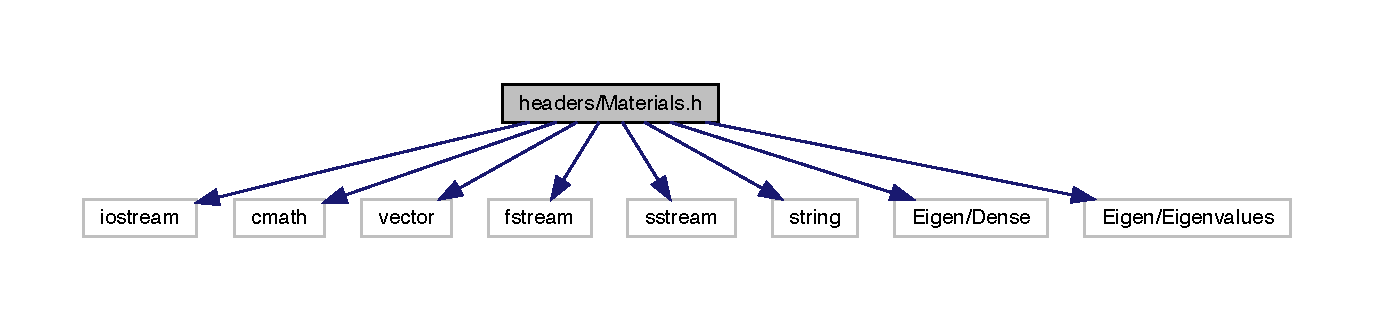
\includegraphics[width=350pt]{_materials_8h__incl}
\end{center}
\end{figure}
This graph shows which files directly or indirectly include this file\+:
\nopagebreak
\begin{figure}[H]
\begin{center}
\leavevmode

\includegraphics[width=350pt]{_materials_8h__dep__incl}
\end{center}
\end{figure}
\subsection*{Classes}
\begin{DoxyCompactItemize}
\item 
class \hyperlink{class_materials}{Materials}
\end{DoxyCompactItemize}

\hypertarget{_mesh_8h}{}\section{headers/\+Mesh.h File Reference}
\label{_mesh_8h}\index{headers/\+Mesh.\+h@{headers/\+Mesh.\+h}}
{\ttfamily \#include $<$iostream$>$}\newline
{\ttfamily \#include $<$cmath$>$}\newline
{\ttfamily \#include $<$vector$>$}\newline
{\ttfamily \#include $<$fstream$>$}\newline
{\ttfamily \#include $<$sstream$>$}\newline
{\ttfamily \#include $<$string$>$}\newline
{\ttfamily \#include \char`\"{}Eigen/\+Dense\char`\"{}}\newline
{\ttfamily \#include \char`\"{}Eigen/\+Eigenvalues\char`\"{}}\newline
Include dependency graph for Mesh.\+h\+:
\nopagebreak
\begin{figure}[H]
\begin{center}
\leavevmode
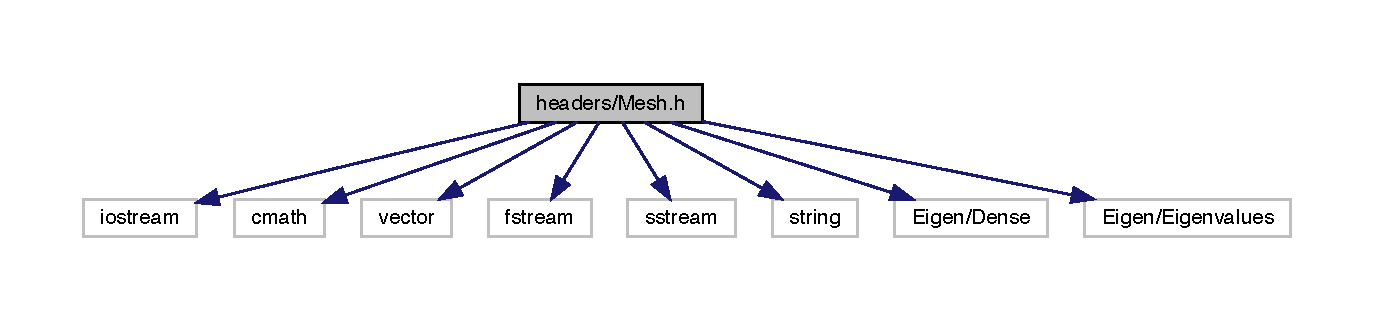
\includegraphics[width=350pt]{_mesh_8h__incl}
\end{center}
\end{figure}
This graph shows which files directly or indirectly include this file\+:
\nopagebreak
\begin{figure}[H]
\begin{center}
\leavevmode

\includegraphics[width=350pt]{_mesh_8h__dep__incl}
\end{center}
\end{figure}
\subsection*{Classes}
\begin{DoxyCompactItemize}
\item 
class \hyperlink{class_mesh}{Mesh}
\end{DoxyCompactItemize}

\hypertarget{main_8cpp}{}\section{main.\+cpp File Reference}
\label{main_8cpp}\index{main.\+cpp@{main.\+cpp}}
{\ttfamily \#include $<$iostream$>$}\newline
{\ttfamily \#include $<$string$>$}\newline
{\ttfamily \#include $<$sstream$>$}\newline
{\ttfamily \#include $<$cmath$>$}\newline
{\ttfamily \#include $<$vector$>$}\newline
{\ttfamily \#include $<$fstream$>$}\newline
{\ttfamily \#include \char`\"{}time.\+h\char`\"{}}\newline
{\ttfamily \#include $<$Eigen/\+Dense$>$}\newline
{\ttfamily \#include \char`\"{}functions.\+h\char`\"{}}\newline
{\ttfamily \#include \char`\"{}Mesh.\+h\char`\"{}}\newline
{\ttfamily \#include \char`\"{}Materials.\+h\char`\"{}}\newline
Include dependency graph for main.\+cpp\+:
\nopagebreak
\begin{figure}[H]
\begin{center}
\leavevmode
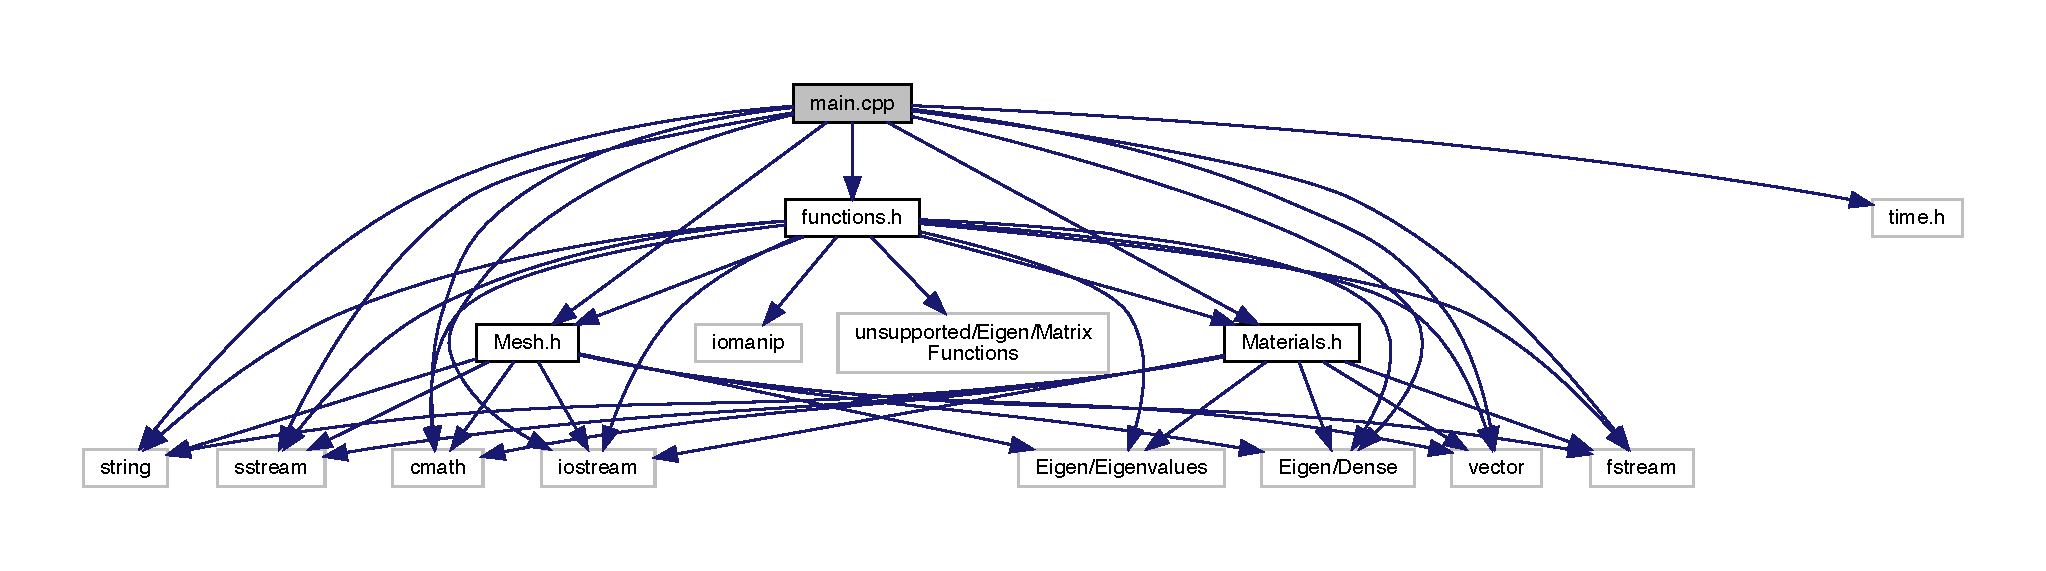
\includegraphics[width=350pt]{main_8cpp__incl}
\end{center}
\end{figure}
\subsection*{Functions}
\begin{DoxyCompactItemize}
\item 
int \hyperlink{main_8cpp_ae66f6b31b5ad750f1fe042a706a4e3d4}{main} ()
\end{DoxyCompactItemize}
\subsection*{Variables}
\begin{DoxyCompactItemize}
\item 
std\+::string \hyperlink{main_8cpp_a556ce46e457f991c51f3dac111579e2b}{home\+\_\+path}
\item 
std\+::string \hyperlink{main_8cpp_a5e3d7c3d50f127de0e61daaa407dc7d1}{job\+\_\+file}
\item 
int \hyperlink{main_8cpp_aa789fe4d8a13fd0990b630909430d5d0}{ndof}
\item 
int \hyperlink{main_8cpp_a509bc84434af1eff0173e4a71bd758ac}{num\+\_\+meshes}
\item 
\hyperlink{class_mesh}{Mesh} $\ast$ \hyperlink{main_8cpp_a6e08f89b32254fb4b129720418e7c6ea}{mesh}
\item 
double \hyperlink{main_8cpp_a1b01a4354147da92a548ea1a5f96d592}{t\+\_\+start}
\item 
double \hyperlink{main_8cpp_a4b637c5fff609e604a3b2b2787f4a9fa}{t\+\_\+end}
\item 
int \hyperlink{main_8cpp_ace6ace9b2f6d8d404ca9e66564289eb1}{output\+\_\+frequency}
\item 
double \hyperlink{main_8cpp_a068c627ac33cf3c721d8f28eab205a83}{dt\+\_\+initial}
\item 
double \hyperlink{main_8cpp_a0a612324885914b6799185d54c48b310}{dt\+\_\+min}
\item 
double \hyperlink{main_8cpp_a7700f3aeb1ca1c9bbbf712dbfb0aa349}{reduction}
\item 
int \hyperlink{main_8cpp_a39328cf72d69139b3b6c5b8ef6c636fe}{material\+\_\+types}
\item 
\hyperlink{class_materials}{Materials} $\ast$ \hyperlink{main_8cpp_acfa6799b35f9301b5fc44e6043624797}{mat}
\item 
int \hyperlink{main_8cpp_a724026f5fcdde8a7ee4936d710ac415d}{num\+\_\+load\+\_\+constraints}
\item 
double \hyperlink{main_8cpp_a41b0f465c44fe8b2de43cfaa05bb7880}{input\+\_\+load\+\_\+amp}
\item 
Vector\+Xi \hyperlink{main_8cpp_ab49fb3bb15f9624e4ffb12a75c7db55d}{fcdof}
\item 
std\+::string \hyperlink{main_8cpp_a51e2def539afa6941aecc0db01966133}{fc\+\_\+curve}
\item 
int \hyperlink{main_8cpp_acfafb3651a4fe2c074c247d95f28635a}{num\+\_\+disp\+\_\+constraints}
\item 
double \hyperlink{main_8cpp_a8610c01521192e9f3677b50b275ff2bf}{input\+\_\+disp\+\_\+amp}
\item 
Vector\+Xi \hyperlink{main_8cpp_a769eb6abca3cfe15c55c120f68bf1461}{dcdof}
\item 
std\+::string \hyperlink{main_8cpp_a7f448b56fa6e59123cfe5fcf0082e8de}{dc\+\_\+curve}
\item 
int \hyperlink{main_8cpp_abd406f244d4145ae5baf4ea059b5232d}{num\+\_\+constraints}
\item 
Vector\+Xi \hyperlink{main_8cpp_a389e085bd7632077f619ea67d3fb4087}{bcdof}
\item 
Vector\+Xd \hyperlink{main_8cpp_a3a53182d9f97dc5acff0a10125857cfb}{bcval}
\item 
Matrix\+Xd \hyperlink{main_8cpp_a6f626bfc805c8f0fb5170c06b4e61c8a}{element\+\_\+stress\+\_\+host}
\item 
Matrix\+Xd \hyperlink{main_8cpp_a1db1555bea7ef22b3783cdd66ebbeb0e}{element\+\_\+strain\+\_\+host}
\item 
Matrix\+Xd \hyperlink{main_8cpp_a1ae14dd64a0bd3139f1e153dc5e48016}{element\+\_\+stress\+\_\+truss}
\item 
Matrix\+Xd \hyperlink{main_8cpp_a296db0b5edbd14e04e368f248587c4eb}{element\+\_\+strain\+\_\+truss}
\item 
Vector\+Xd \hyperlink{main_8cpp_ae07dc1b145ffa9093a4262baf26aff7a}{fi\+\_\+prev}
\item 
Vector\+Xd \hyperlink{main_8cpp_a7a1410ed488bb0dd5c10344c4c4951e6}{fi\+\_\+curr}
\item 
Vector\+Xd \hyperlink{main_8cpp_a3ebb0eb4b098a0ac9e1f24de934a282f}{W\+\_\+int}
\item 
Vector\+Xd \hyperlink{main_8cpp_a032d9f703d3d55ca1e54f14f44457615}{U\+\_\+host}
\item 
Vector\+Xd \hyperlink{main_8cpp_ad72fa62a83a5fde880ab78c8c81c48bb}{V\+\_\+host}
\item 
Vector\+Xd \hyperlink{main_8cpp_a7a1e6ce58aaa0309efd50328e8f295e9}{A\+\_\+host}
\item 
Vector\+Xd \hyperlink{main_8cpp_a94430566d55ccfa65e497716fd404dea}{U\+\_\+truss}
\item 
Vector\+Xd \hyperlink{main_8cpp_a5159843113dbbfc6e912c3345c0a7916}{V\+\_\+truss}
\item 
Vector\+Xd \hyperlink{main_8cpp_a2f98cf28208251affb988effe3a89708}{A\+\_\+truss}
\item 
double \hyperlink{main_8cpp_ad3d80cd8d6370090eb6cc57a523bcd6c}{eps\+\_\+nr}
\item 
double \hyperlink{main_8cpp_a43f0d7a4e9f3ece65db80d07bb79192f}{iterations\+\_\+nr}
\end{DoxyCompactItemize}


\subsection{Function Documentation}
\mbox{\Hypertarget{main_8cpp_ae66f6b31b5ad750f1fe042a706a4e3d4}\label{main_8cpp_ae66f6b31b5ad750f1fe042a706a4e3d4}} 
\index{main.\+cpp@{main.\+cpp}!main@{main}}
\index{main@{main}!main.\+cpp@{main.\+cpp}}
\subsubsection{\texorpdfstring{main()}{main()}}
{\footnotesize\ttfamily int main (\begin{DoxyParamCaption}{ }\end{DoxyParamCaption})}

This is the main file. If you want to submit a new job -- this is where you do it Constants used in the code

Enter the path address for your job folder

What is the Problem Dimension -\/ Degrees of Freedom per node?

Simulation start time

Simulation end time

Output frequency -- result ouputs for every 100 timesteps

Maximum time step

Reduction factor

Type of Loading 1 -\/ Force based 2 -\/ Displacement based

Loading Amplitude

number of nodes $\ast$ number of directions

Degrees of freedom index data

Number of boundary condition constraints

Which nodes are constrained ?

index corresponding to the constrained degrees of freedom

Displacements of the constrained degrees of freedom

Enter your choice for type of simulations below, based on the following options\+: 1 -\/ Explicit Dynamic 2 -\/ Implicit Dynamic 3 -\/ Static Analysis

Definition at line 119 of file main.\+cpp.

Here is the call graph for this function\+:
\nopagebreak
\begin{figure}[H]
\begin{center}
\leavevmode
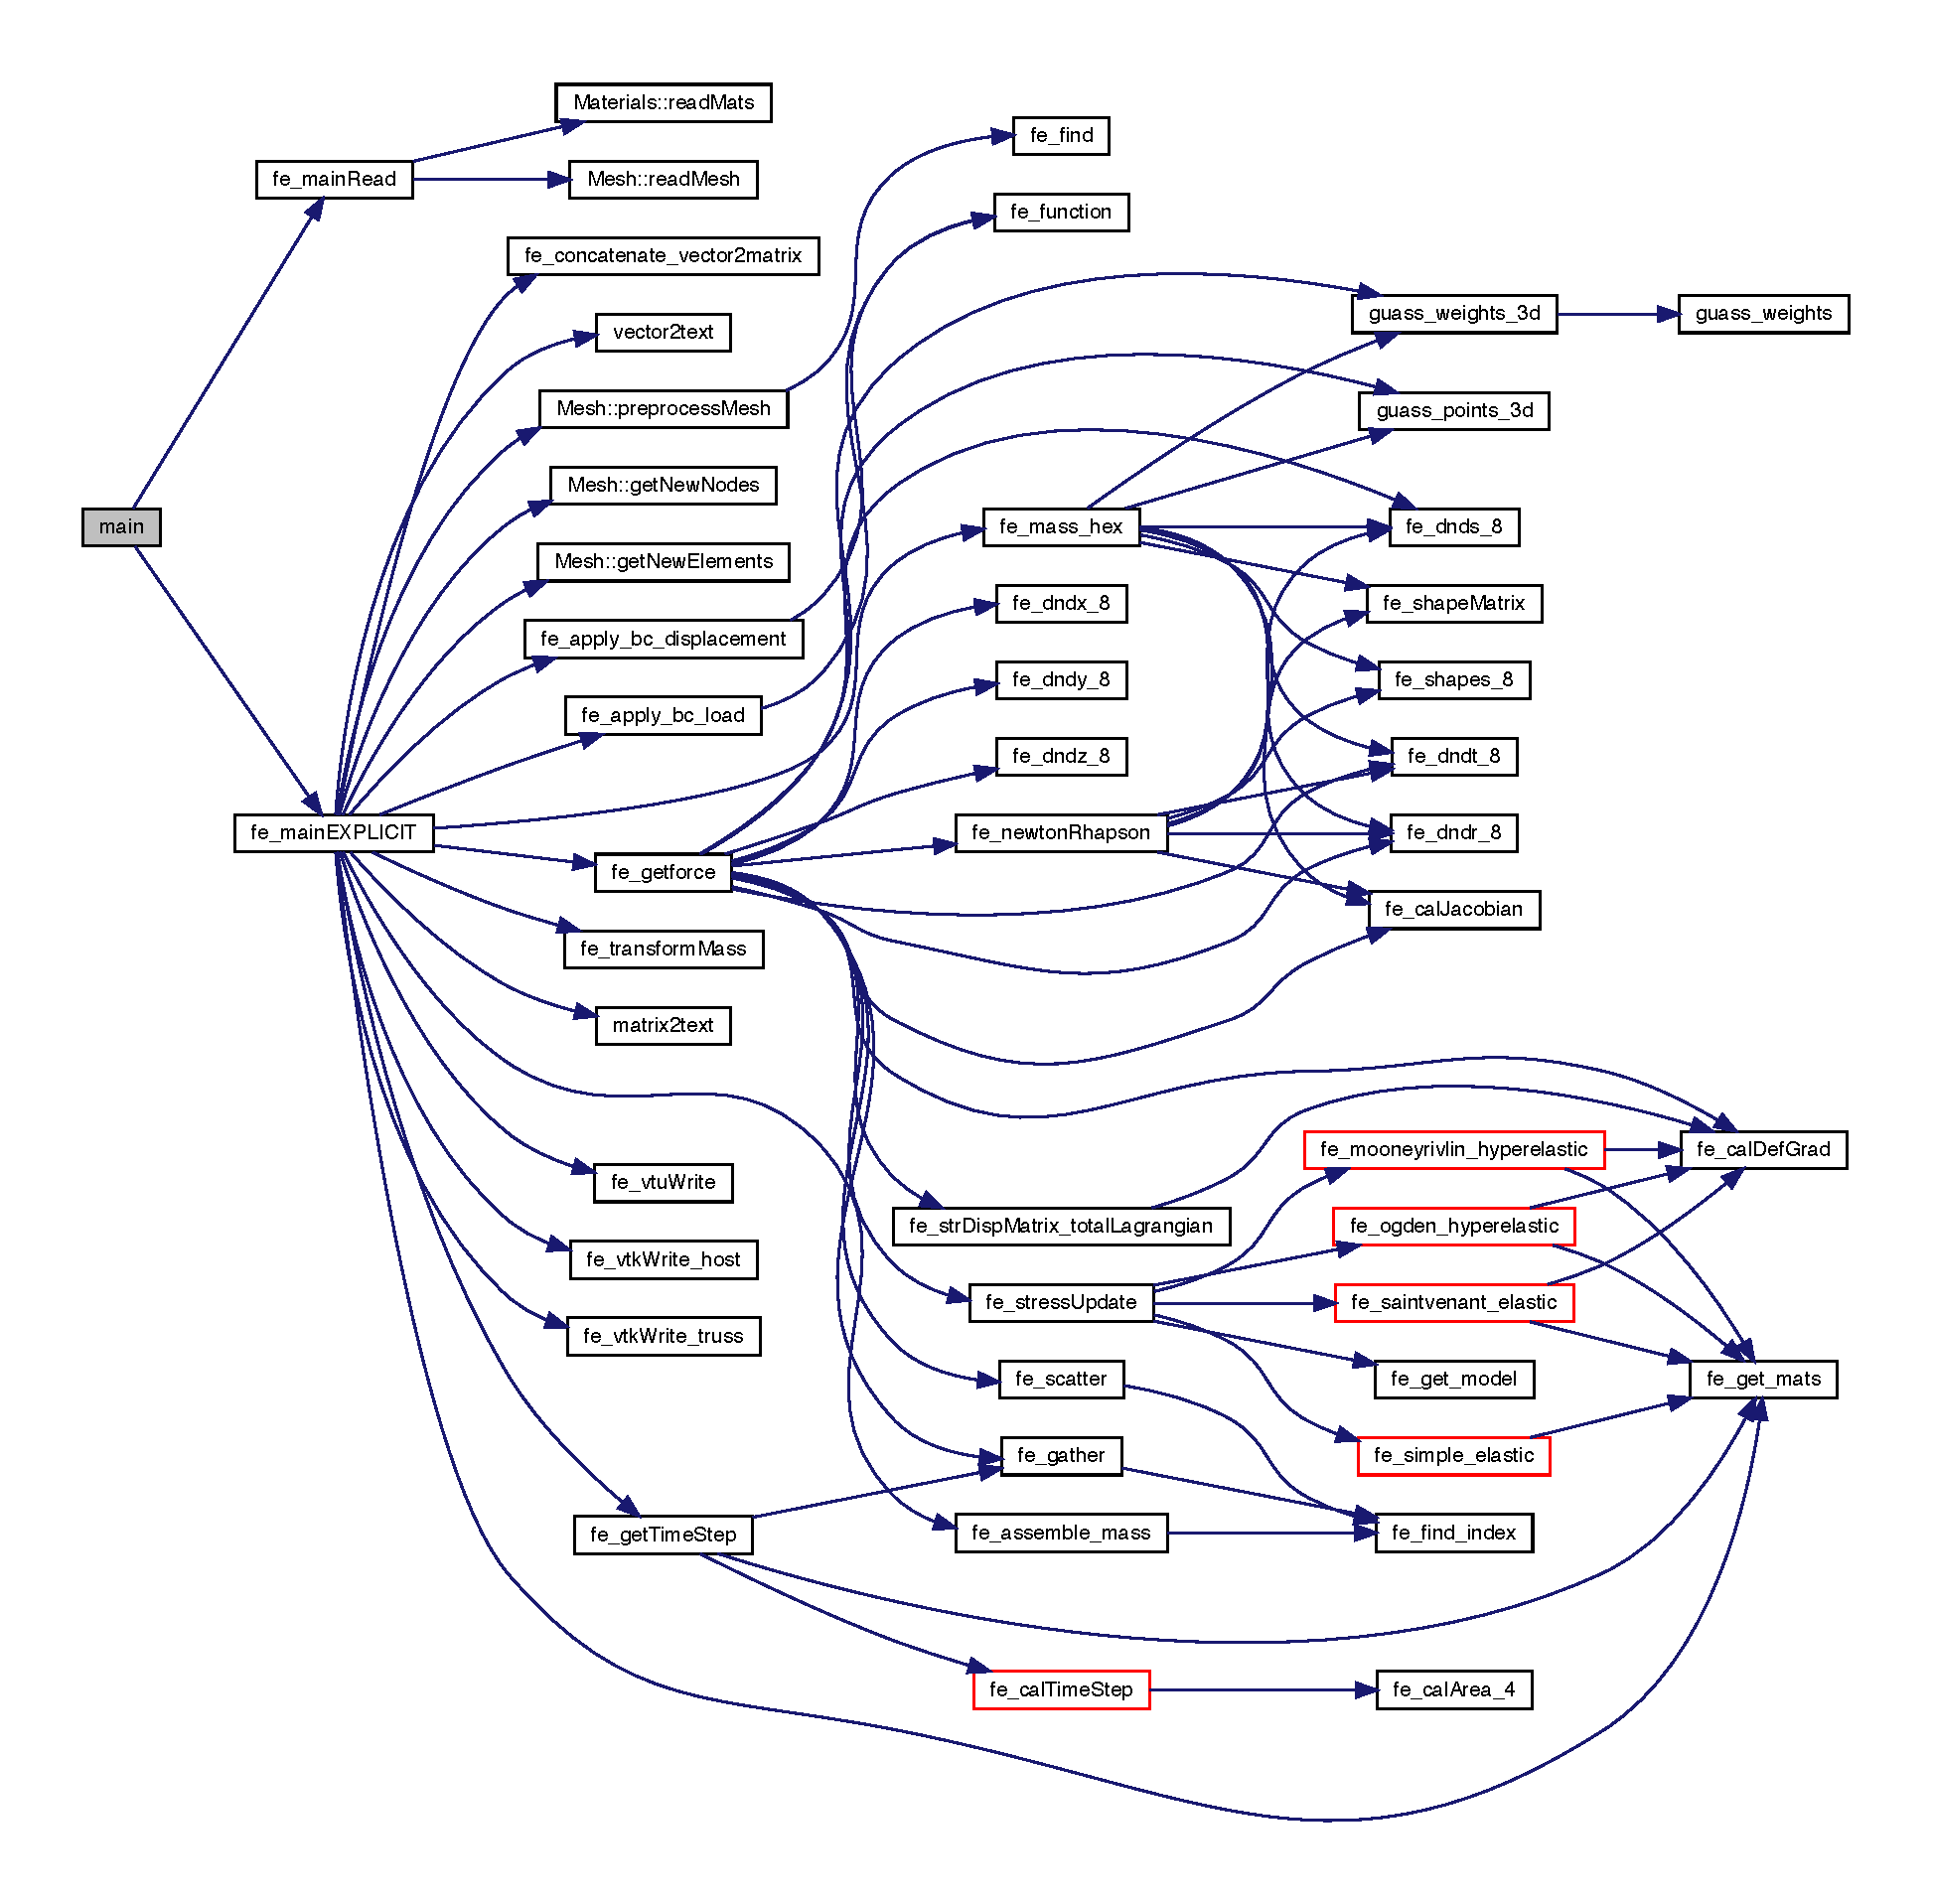
\includegraphics[width=350pt]{main_8cpp_ae66f6b31b5ad750f1fe042a706a4e3d4_cgraph}
\end{center}
\end{figure}


\subsection{Variable Documentation}
\mbox{\Hypertarget{main_8cpp_a7a1e6ce58aaa0309efd50328e8f295e9}\label{main_8cpp_a7a1e6ce58aaa0309efd50328e8f295e9}} 
\index{main.\+cpp@{main.\+cpp}!A\+\_\+host@{A\+\_\+host}}
\index{A\+\_\+host@{A\+\_\+host}!main.\+cpp@{main.\+cpp}}
\subsubsection{\texorpdfstring{A\+\_\+host}{A\_host}}
{\footnotesize\ttfamily Vector\+Xd A\+\_\+host}

Variable storing the nodal velocities of the host mesh 

Definition at line 106 of file main.\+cpp.

\mbox{\Hypertarget{main_8cpp_a2f98cf28208251affb988effe3a89708}\label{main_8cpp_a2f98cf28208251affb988effe3a89708}} 
\index{main.\+cpp@{main.\+cpp}!A\+\_\+truss@{A\+\_\+truss}}
\index{A\+\_\+truss@{A\+\_\+truss}!main.\+cpp@{main.\+cpp}}
\subsubsection{\texorpdfstring{A\+\_\+truss}{A\_truss}}
{\footnotesize\ttfamily Vector\+Xd A\+\_\+truss}

Variable storing the nodal velocities of the embedded mesh 

Definition at line 110 of file main.\+cpp.

\mbox{\Hypertarget{main_8cpp_a389e085bd7632077f619ea67d3fb4087}\label{main_8cpp_a389e085bd7632077f619ea67d3fb4087}} 
\index{main.\+cpp@{main.\+cpp}!bcdof@{bcdof}}
\index{bcdof@{bcdof}!main.\+cpp@{main.\+cpp}}
\subsubsection{\texorpdfstring{bcdof}{bcdof}}
{\footnotesize\ttfamily Vector\+Xi bcdof}

D\+OF numbers for boundary conditions 

Definition at line 88 of file main.\+cpp.

\mbox{\Hypertarget{main_8cpp_a3a53182d9f97dc5acff0a10125857cfb}\label{main_8cpp_a3a53182d9f97dc5acff0a10125857cfb}} 
\index{main.\+cpp@{main.\+cpp}!bcval@{bcval}}
\index{bcval@{bcval}!main.\+cpp@{main.\+cpp}}
\subsubsection{\texorpdfstring{bcval}{bcval}}
{\footnotesize\ttfamily Vector\+Xd bcval}

Displacement of the constrained D\+OF\textquotesingle{}s 

Definition at line 90 of file main.\+cpp.

\mbox{\Hypertarget{main_8cpp_a7f448b56fa6e59123cfe5fcf0082e8de}\label{main_8cpp_a7f448b56fa6e59123cfe5fcf0082e8de}} 
\index{main.\+cpp@{main.\+cpp}!dc\+\_\+curve@{dc\+\_\+curve}}
\index{dc\+\_\+curve@{dc\+\_\+curve}!main.\+cpp@{main.\+cpp}}
\subsubsection{\texorpdfstring{dc\+\_\+curve}{dc\_curve}}
{\footnotesize\ttfamily std\+::string dc\+\_\+curve}



Definition at line 82 of file main.\+cpp.

\mbox{\Hypertarget{main_8cpp_a769eb6abca3cfe15c55c120f68bf1461}\label{main_8cpp_a769eb6abca3cfe15c55c120f68bf1461}} 
\index{main.\+cpp@{main.\+cpp}!dcdof@{dcdof}}
\index{dcdof@{dcdof}!main.\+cpp@{main.\+cpp}}
\subsubsection{\texorpdfstring{dcdof}{dcdof}}
{\footnotesize\ttfamily Vector\+Xi dcdof}



Definition at line 81 of file main.\+cpp.

\mbox{\Hypertarget{main_8cpp_a068c627ac33cf3c721d8f28eab205a83}\label{main_8cpp_a068c627ac33cf3c721d8f28eab205a83}} 
\index{main.\+cpp@{main.\+cpp}!dt\+\_\+initial@{dt\+\_\+initial}}
\index{dt\+\_\+initial@{dt\+\_\+initial}!main.\+cpp@{main.\+cpp}}
\subsubsection{\texorpdfstring{dt\+\_\+initial}{dt\_initial}}
{\footnotesize\ttfamily double dt\+\_\+initial}



Definition at line 66 of file main.\+cpp.

\mbox{\Hypertarget{main_8cpp_a0a612324885914b6799185d54c48b310}\label{main_8cpp_a0a612324885914b6799185d54c48b310}} 
\index{main.\+cpp@{main.\+cpp}!dt\+\_\+min@{dt\+\_\+min}}
\index{dt\+\_\+min@{dt\+\_\+min}!main.\+cpp@{main.\+cpp}}
\subsubsection{\texorpdfstring{dt\+\_\+min}{dt\_min}}
{\footnotesize\ttfamily double dt\+\_\+min}

Initial time step 

Definition at line 67 of file main.\+cpp.

\mbox{\Hypertarget{main_8cpp_a1db1555bea7ef22b3783cdd66ebbeb0e}\label{main_8cpp_a1db1555bea7ef22b3783cdd66ebbeb0e}} 
\index{main.\+cpp@{main.\+cpp}!element\+\_\+strain\+\_\+host@{element\+\_\+strain\+\_\+host}}
\index{element\+\_\+strain\+\_\+host@{element\+\_\+strain\+\_\+host}!main.\+cpp@{main.\+cpp}}
\subsubsection{\texorpdfstring{element\+\_\+strain\+\_\+host}{element\_strain\_host}}
{\footnotesize\ttfamily Matrix\+Xd element\+\_\+strain\+\_\+host}

Stores the stress tensor of an element 

Definition at line 94 of file main.\+cpp.

\mbox{\Hypertarget{main_8cpp_a296db0b5edbd14e04e368f248587c4eb}\label{main_8cpp_a296db0b5edbd14e04e368f248587c4eb}} 
\index{main.\+cpp@{main.\+cpp}!element\+\_\+strain\+\_\+truss@{element\+\_\+strain\+\_\+truss}}
\index{element\+\_\+strain\+\_\+truss@{element\+\_\+strain\+\_\+truss}!main.\+cpp@{main.\+cpp}}
\subsubsection{\texorpdfstring{element\+\_\+strain\+\_\+truss}{element\_strain\_truss}}
{\footnotesize\ttfamily Matrix\+Xd element\+\_\+strain\+\_\+truss}

Stores the stress of a truss element 

Definition at line 96 of file main.\+cpp.

\mbox{\Hypertarget{main_8cpp_a6f626bfc805c8f0fb5170c06b4e61c8a}\label{main_8cpp_a6f626bfc805c8f0fb5170c06b4e61c8a}} 
\index{main.\+cpp@{main.\+cpp}!element\+\_\+stress\+\_\+host@{element\+\_\+stress\+\_\+host}}
\index{element\+\_\+stress\+\_\+host@{element\+\_\+stress\+\_\+host}!main.\+cpp@{main.\+cpp}}
\subsubsection{\texorpdfstring{element\+\_\+stress\+\_\+host}{element\_stress\_host}}
{\footnotesize\ttfamily Matrix\+Xd element\+\_\+stress\+\_\+host}



Definition at line 93 of file main.\+cpp.

\mbox{\Hypertarget{main_8cpp_a1ae14dd64a0bd3139f1e153dc5e48016}\label{main_8cpp_a1ae14dd64a0bd3139f1e153dc5e48016}} 
\index{main.\+cpp@{main.\+cpp}!element\+\_\+stress\+\_\+truss@{element\+\_\+stress\+\_\+truss}}
\index{element\+\_\+stress\+\_\+truss@{element\+\_\+stress\+\_\+truss}!main.\+cpp@{main.\+cpp}}
\subsubsection{\texorpdfstring{element\+\_\+stress\+\_\+truss}{element\_stress\_truss}}
{\footnotesize\ttfamily Matrix\+Xd element\+\_\+stress\+\_\+truss}

Stores the strain tensor of an element 

Definition at line 95 of file main.\+cpp.

\mbox{\Hypertarget{main_8cpp_ad3d80cd8d6370090eb6cc57a523bcd6c}\label{main_8cpp_ad3d80cd8d6370090eb6cc57a523bcd6c}} 
\index{main.\+cpp@{main.\+cpp}!eps\+\_\+nr@{eps\+\_\+nr}}
\index{eps\+\_\+nr@{eps\+\_\+nr}!main.\+cpp@{main.\+cpp}}
\subsubsection{\texorpdfstring{eps\+\_\+nr}{eps\_nr}}
{\footnotesize\ttfamily double eps\+\_\+nr}

Variable storing the nodal accelerations of the embedded mesh 

Definition at line 112 of file main.\+cpp.

\mbox{\Hypertarget{main_8cpp_a51e2def539afa6941aecc0db01966133}\label{main_8cpp_a51e2def539afa6941aecc0db01966133}} 
\index{main.\+cpp@{main.\+cpp}!fc\+\_\+curve@{fc\+\_\+curve}}
\index{fc\+\_\+curve@{fc\+\_\+curve}!main.\+cpp@{main.\+cpp}}
\subsubsection{\texorpdfstring{fc\+\_\+curve}{fc\_curve}}
{\footnotesize\ttfamily std\+::string fc\+\_\+curve}

Degrees of freedom -- corresponding to the applied load 

Definition at line 77 of file main.\+cpp.

\mbox{\Hypertarget{main_8cpp_ab49fb3bb15f9624e4ffb12a75c7db55d}\label{main_8cpp_ab49fb3bb15f9624e4ffb12a75c7db55d}} 
\index{main.\+cpp@{main.\+cpp}!fcdof@{fcdof}}
\index{fcdof@{fcdof}!main.\+cpp@{main.\+cpp}}
\subsubsection{\texorpdfstring{fcdof}{fcdof}}
{\footnotesize\ttfamily Vector\+Xi fcdof}

Loading Amplitude 

Definition at line 76 of file main.\+cpp.

\mbox{\Hypertarget{main_8cpp_a7a1410ed488bb0dd5c10344c4c4951e6}\label{main_8cpp_a7a1410ed488bb0dd5c10344c4c4951e6}} 
\index{main.\+cpp@{main.\+cpp}!fi\+\_\+curr@{fi\+\_\+curr}}
\index{fi\+\_\+curr@{fi\+\_\+curr}!main.\+cpp@{main.\+cpp}}
\subsubsection{\texorpdfstring{fi\+\_\+curr}{fi\_curr}}
{\footnotesize\ttfamily Vector\+Xd fi\+\_\+curr}

Internal nodal force vector at previous time step 

Definition at line 101 of file main.\+cpp.

\mbox{\Hypertarget{main_8cpp_ae07dc1b145ffa9093a4262baf26aff7a}\label{main_8cpp_ae07dc1b145ffa9093a4262baf26aff7a}} 
\index{main.\+cpp@{main.\+cpp}!fi\+\_\+prev@{fi\+\_\+prev}}
\index{fi\+\_\+prev@{fi\+\_\+prev}!main.\+cpp@{main.\+cpp}}
\subsubsection{\texorpdfstring{fi\+\_\+prev}{fi\_prev}}
{\footnotesize\ttfamily Vector\+Xd fi\+\_\+prev}

Stores the strain of a truss element 

Definition at line 100 of file main.\+cpp.

\mbox{\Hypertarget{main_8cpp_a556ce46e457f991c51f3dac111579e2b}\label{main_8cpp_a556ce46e457f991c51f3dac111579e2b}} 
\index{main.\+cpp@{main.\+cpp}!home\+\_\+path@{home\+\_\+path}}
\index{home\+\_\+path@{home\+\_\+path}!main.\+cpp@{main.\+cpp}}
\subsubsection{\texorpdfstring{home\+\_\+path}{home\_path}}
{\footnotesize\ttfamily std\+::string home\+\_\+path}



Definition at line 52 of file main.\+cpp.

\mbox{\Hypertarget{main_8cpp_a8610c01521192e9f3677b50b275ff2bf}\label{main_8cpp_a8610c01521192e9f3677b50b275ff2bf}} 
\index{main.\+cpp@{main.\+cpp}!input\+\_\+disp\+\_\+amp@{input\+\_\+disp\+\_\+amp}}
\index{input\+\_\+disp\+\_\+amp@{input\+\_\+disp\+\_\+amp}!main.\+cpp@{main.\+cpp}}
\subsubsection{\texorpdfstring{input\+\_\+disp\+\_\+amp}{input\_disp\_amp}}
{\footnotesize\ttfamily double input\+\_\+disp\+\_\+amp}



Definition at line 80 of file main.\+cpp.

\mbox{\Hypertarget{main_8cpp_a41b0f465c44fe8b2de43cfaa05bb7880}\label{main_8cpp_a41b0f465c44fe8b2de43cfaa05bb7880}} 
\index{main.\+cpp@{main.\+cpp}!input\+\_\+load\+\_\+amp@{input\+\_\+load\+\_\+amp}}
\index{input\+\_\+load\+\_\+amp@{input\+\_\+load\+\_\+amp}!main.\+cpp@{main.\+cpp}}
\subsubsection{\texorpdfstring{input\+\_\+load\+\_\+amp}{input\_load\_amp}}
{\footnotesize\ttfamily double input\+\_\+load\+\_\+amp}



Definition at line 75 of file main.\+cpp.

\mbox{\Hypertarget{main_8cpp_a43f0d7a4e9f3ece65db80d07bb79192f}\label{main_8cpp_a43f0d7a4e9f3ece65db80d07bb79192f}} 
\index{main.\+cpp@{main.\+cpp}!iterations\+\_\+nr@{iterations\+\_\+nr}}
\index{iterations\+\_\+nr@{iterations\+\_\+nr}!main.\+cpp@{main.\+cpp}}
\subsubsection{\texorpdfstring{iterations\+\_\+nr}{iterations\_nr}}
{\footnotesize\ttfamily double iterations\+\_\+nr}

Convergence criteria used in the newton rhapson method 

Definition at line 113 of file main.\+cpp.

\mbox{\Hypertarget{main_8cpp_a5e3d7c3d50f127de0e61daaa407dc7d1}\label{main_8cpp_a5e3d7c3d50f127de0e61daaa407dc7d1}} 
\index{main.\+cpp@{main.\+cpp}!job\+\_\+file@{job\+\_\+file}}
\index{job\+\_\+file@{job\+\_\+file}!main.\+cpp@{main.\+cpp}}
\subsubsection{\texorpdfstring{job\+\_\+file}{job\_file}}
{\footnotesize\ttfamily std\+::string job\+\_\+file}

Job folder name 

Definition at line 53 of file main.\+cpp.

\mbox{\Hypertarget{main_8cpp_acfa6799b35f9301b5fc44e6043624797}\label{main_8cpp_acfa6799b35f9301b5fc44e6043624797}} 
\index{main.\+cpp@{main.\+cpp}!mat@{mat}}
\index{mat@{mat}!main.\+cpp@{main.\+cpp}}
\subsubsection{\texorpdfstring{mat}{mat}}
{\footnotesize\ttfamily \hyperlink{class_materials}{Materials}$\ast$ mat}



Definition at line 72 of file main.\+cpp.

\mbox{\Hypertarget{main_8cpp_a39328cf72d69139b3b6c5b8ef6c636fe}\label{main_8cpp_a39328cf72d69139b3b6c5b8ef6c636fe}} 
\index{main.\+cpp@{main.\+cpp}!material\+\_\+types@{material\+\_\+types}}
\index{material\+\_\+types@{material\+\_\+types}!main.\+cpp@{main.\+cpp}}
\subsubsection{\texorpdfstring{material\+\_\+types}{material\_types}}
{\footnotesize\ttfamily int material\+\_\+types}

Reduces the timestep value by this amount Material Properties are stored in here 

Definition at line 71 of file main.\+cpp.

\mbox{\Hypertarget{main_8cpp_a6e08f89b32254fb4b129720418e7c6ea}\label{main_8cpp_a6e08f89b32254fb4b129720418e7c6ea}} 
\index{main.\+cpp@{main.\+cpp}!mesh@{mesh}}
\index{mesh@{mesh}!main.\+cpp@{main.\+cpp}}
\subsubsection{\texorpdfstring{mesh}{mesh}}
{\footnotesize\ttfamily \hyperlink{class_mesh}{Mesh}$\ast$ mesh}



Definition at line 60 of file main.\+cpp.

\mbox{\Hypertarget{main_8cpp_aa789fe4d8a13fd0990b630909430d5d0}\label{main_8cpp_aa789fe4d8a13fd0990b630909430d5d0}} 
\index{main.\+cpp@{main.\+cpp}!ndof@{ndof}}
\index{ndof@{ndof}!main.\+cpp@{main.\+cpp}}
\subsubsection{\texorpdfstring{ndof}{ndof}}
{\footnotesize\ttfamily int ndof}

Job input file name Dimension of the Simulation (3 for 3D, 2 for 2D and 1 for 1D) 

Definition at line 56 of file main.\+cpp.

\mbox{\Hypertarget{main_8cpp_abd406f244d4145ae5baf4ea059b5232d}\label{main_8cpp_abd406f244d4145ae5baf4ea059b5232d}} 
\index{main.\+cpp@{main.\+cpp}!num\+\_\+constraints@{num\+\_\+constraints}}
\index{num\+\_\+constraints@{num\+\_\+constraints}!main.\+cpp@{main.\+cpp}}
\subsubsection{\texorpdfstring{num\+\_\+constraints}{num\_constraints}}
{\footnotesize\ttfamily int num\+\_\+constraints}

Type of displacement curve Number of boundary conditions = nodes x dof 

Definition at line 86 of file main.\+cpp.

\mbox{\Hypertarget{main_8cpp_acfafb3651a4fe2c074c247d95f28635a}\label{main_8cpp_acfafb3651a4fe2c074c247d95f28635a}} 
\index{main.\+cpp@{main.\+cpp}!num\+\_\+disp\+\_\+constraints@{num\+\_\+disp\+\_\+constraints}}
\index{num\+\_\+disp\+\_\+constraints@{num\+\_\+disp\+\_\+constraints}!main.\+cpp@{main.\+cpp}}
\subsubsection{\texorpdfstring{num\+\_\+disp\+\_\+constraints}{num\_disp\_constraints}}
{\footnotesize\ttfamily int num\+\_\+disp\+\_\+constraints}

Type of loading curve 

Definition at line 79 of file main.\+cpp.

\mbox{\Hypertarget{main_8cpp_a724026f5fcdde8a7ee4936d710ac415d}\label{main_8cpp_a724026f5fcdde8a7ee4936d710ac415d}} 
\index{main.\+cpp@{main.\+cpp}!num\+\_\+load\+\_\+constraints@{num\+\_\+load\+\_\+constraints}}
\index{num\+\_\+load\+\_\+constraints@{num\+\_\+load\+\_\+constraints}!main.\+cpp@{main.\+cpp}}
\subsubsection{\texorpdfstring{num\+\_\+load\+\_\+constraints}{num\_load\_constraints}}
{\footnotesize\ttfamily int num\+\_\+load\+\_\+constraints}



Definition at line 74 of file main.\+cpp.

\mbox{\Hypertarget{main_8cpp_a509bc84434af1eff0173e4a71bd758ac}\label{main_8cpp_a509bc84434af1eff0173e4a71bd758ac}} 
\index{main.\+cpp@{main.\+cpp}!num\+\_\+meshes@{num\+\_\+meshes}}
\index{num\+\_\+meshes@{num\+\_\+meshes}!main.\+cpp@{main.\+cpp}}
\subsubsection{\texorpdfstring{num\+\_\+meshes}{num\_meshes}}
{\footnotesize\ttfamily int num\+\_\+meshes}

Input meshes -\/ number of meshes and type of meshes 

Definition at line 59 of file main.\+cpp.

\mbox{\Hypertarget{main_8cpp_ace6ace9b2f6d8d404ca9e66564289eb1}\label{main_8cpp_ace6ace9b2f6d8d404ca9e66564289eb1}} 
\index{main.\+cpp@{main.\+cpp}!output\+\_\+frequency@{output\+\_\+frequency}}
\index{output\+\_\+frequency@{output\+\_\+frequency}!main.\+cpp@{main.\+cpp}}
\subsubsection{\texorpdfstring{output\+\_\+frequency}{output\_frequency}}
{\footnotesize\ttfamily int output\+\_\+frequency}

End Time 

Definition at line 65 of file main.\+cpp.

\mbox{\Hypertarget{main_8cpp_a7700f3aeb1ca1c9bbbf712dbfb0aa349}\label{main_8cpp_a7700f3aeb1ca1c9bbbf712dbfb0aa349}} 
\index{main.\+cpp@{main.\+cpp}!reduction@{reduction}}
\index{reduction@{reduction}!main.\+cpp@{main.\+cpp}}
\subsubsection{\texorpdfstring{reduction}{reduction}}
{\footnotesize\ttfamily double reduction}

Minimum time step 

Definition at line 68 of file main.\+cpp.

\mbox{\Hypertarget{main_8cpp_a4b637c5fff609e604a3b2b2787f4a9fa}\label{main_8cpp_a4b637c5fff609e604a3b2b2787f4a9fa}} 
\index{main.\+cpp@{main.\+cpp}!t\+\_\+end@{t\+\_\+end}}
\index{t\+\_\+end@{t\+\_\+end}!main.\+cpp@{main.\+cpp}}
\subsubsection{\texorpdfstring{t\+\_\+end}{t\_end}}
{\footnotesize\ttfamily double t\+\_\+end}

Start Time 

Definition at line 64 of file main.\+cpp.

\mbox{\Hypertarget{main_8cpp_a1b01a4354147da92a548ea1a5f96d592}\label{main_8cpp_a1b01a4354147da92a548ea1a5f96d592}} 
\index{main.\+cpp@{main.\+cpp}!t\+\_\+start@{t\+\_\+start}}
\index{t\+\_\+start@{t\+\_\+start}!main.\+cpp@{main.\+cpp}}
\subsubsection{\texorpdfstring{t\+\_\+start}{t\_start}}
{\footnotesize\ttfamily double t\+\_\+start}



Definition at line 63 of file main.\+cpp.

\mbox{\Hypertarget{main_8cpp_a032d9f703d3d55ca1e54f14f44457615}\label{main_8cpp_a032d9f703d3d55ca1e54f14f44457615}} 
\index{main.\+cpp@{main.\+cpp}!U\+\_\+host@{U\+\_\+host}}
\index{U\+\_\+host@{U\+\_\+host}!main.\+cpp@{main.\+cpp}}
\subsubsection{\texorpdfstring{U\+\_\+host}{U\_host}}
{\footnotesize\ttfamily Vector\+Xd U\+\_\+host}

Internal energy at different time steps 

Definition at line 104 of file main.\+cpp.

\mbox{\Hypertarget{main_8cpp_a94430566d55ccfa65e497716fd404dea}\label{main_8cpp_a94430566d55ccfa65e497716fd404dea}} 
\index{main.\+cpp@{main.\+cpp}!U\+\_\+truss@{U\+\_\+truss}}
\index{U\+\_\+truss@{U\+\_\+truss}!main.\+cpp@{main.\+cpp}}
\subsubsection{\texorpdfstring{U\+\_\+truss}{U\_truss}}
{\footnotesize\ttfamily Vector\+Xd U\+\_\+truss}

Variable storing the nodal accelerations of the host mesh 

Definition at line 108 of file main.\+cpp.

\mbox{\Hypertarget{main_8cpp_ad72fa62a83a5fde880ab78c8c81c48bb}\label{main_8cpp_ad72fa62a83a5fde880ab78c8c81c48bb}} 
\index{main.\+cpp@{main.\+cpp}!V\+\_\+host@{V\+\_\+host}}
\index{V\+\_\+host@{V\+\_\+host}!main.\+cpp@{main.\+cpp}}
\subsubsection{\texorpdfstring{V\+\_\+host}{V\_host}}
{\footnotesize\ttfamily Vector\+Xd V\+\_\+host}

Variable storing the nodal displacements of the host mesh 

Definition at line 105 of file main.\+cpp.

\mbox{\Hypertarget{main_8cpp_a5159843113dbbfc6e912c3345c0a7916}\label{main_8cpp_a5159843113dbbfc6e912c3345c0a7916}} 
\index{main.\+cpp@{main.\+cpp}!V\+\_\+truss@{V\+\_\+truss}}
\index{V\+\_\+truss@{V\+\_\+truss}!main.\+cpp@{main.\+cpp}}
\subsubsection{\texorpdfstring{V\+\_\+truss}{V\_truss}}
{\footnotesize\ttfamily Vector\+Xd V\+\_\+truss}

Variable storing the nodal displacements of the embedded mesh 

Definition at line 109 of file main.\+cpp.

\mbox{\Hypertarget{main_8cpp_a3ebb0eb4b098a0ac9e1f24de934a282f}\label{main_8cpp_a3ebb0eb4b098a0ac9e1f24de934a282f}} 
\index{main.\+cpp@{main.\+cpp}!W\+\_\+int@{W\+\_\+int}}
\index{W\+\_\+int@{W\+\_\+int}!main.\+cpp@{main.\+cpp}}
\subsubsection{\texorpdfstring{W\+\_\+int}{W\_int}}
{\footnotesize\ttfamily Vector\+Xd W\+\_\+int}

Internal nodal force vector at current time step 

Definition at line 102 of file main.\+cpp.


\hypertarget{_r_e_a_d_m_e_8md}{}\section{R\+E\+A\+D\+M\+E.\+md File Reference}
\label{_r_e_a_d_m_e_8md}\index{R\+E\+A\+D\+M\+E.\+md@{R\+E\+A\+D\+M\+E.\+md}}

\hypertarget{fe__cal_def_grad_8cpp}{}\section{source/\+Elements/\+Element\+Calculations/fe\+\_\+cal\+Def\+Grad.cpp File Reference}
\label{fe__cal_def_grad_8cpp}\index{source/\+Elements/\+Element\+Calculations/fe\+\_\+cal\+Def\+Grad.\+cpp@{source/\+Elements/\+Element\+Calculations/fe\+\_\+cal\+Def\+Grad.\+cpp}}
{\ttfamily \#include \char`\"{}functions.\+h\char`\"{}}\newline
Include dependency graph for fe\+\_\+cal\+Def\+Grad.\+cpp\+:
\nopagebreak
\begin{figure}[H]
\begin{center}
\leavevmode
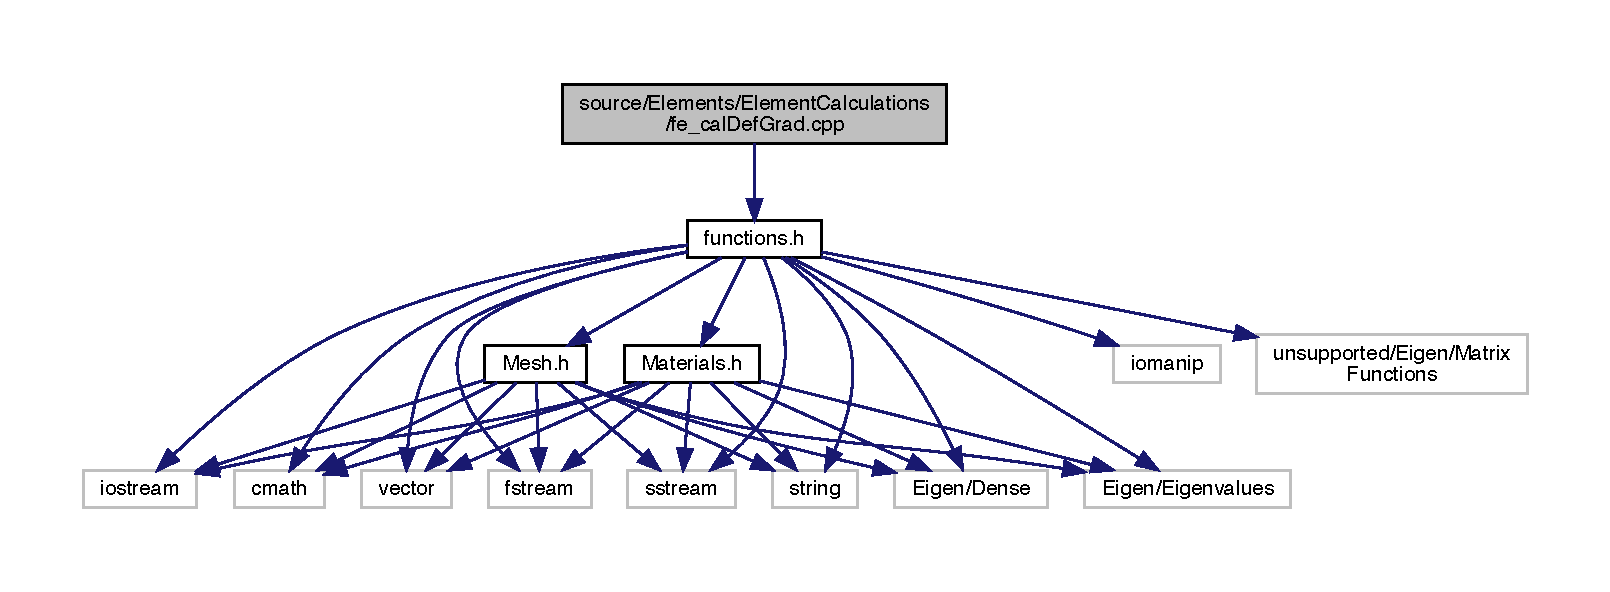
\includegraphics[width=350pt]{fe__cal_def_grad_8cpp__incl}
\end{center}
\end{figure}
\subsection*{Functions}
\begin{DoxyCompactItemize}
\item 
Matrix\+Xd \hyperlink{fe__cal_def_grad_8cpp_ae50379f74802347e04dbc022897f9cb0}{fe\+\_\+cal\+Def\+Grad} (Vector\+Xd dndx, Vector\+Xd dndy, Vector\+Xd dndz, Vector\+Xd u)
\end{DoxyCompactItemize}


\subsection{Function Documentation}
\mbox{\Hypertarget{fe__cal_def_grad_8cpp_ae50379f74802347e04dbc022897f9cb0}\label{fe__cal_def_grad_8cpp_ae50379f74802347e04dbc022897f9cb0}} 
\index{fe\+\_\+cal\+Def\+Grad.\+cpp@{fe\+\_\+cal\+Def\+Grad.\+cpp}!fe\+\_\+cal\+Def\+Grad@{fe\+\_\+cal\+Def\+Grad}}
\index{fe\+\_\+cal\+Def\+Grad@{fe\+\_\+cal\+Def\+Grad}!fe\+\_\+cal\+Def\+Grad.\+cpp@{fe\+\_\+cal\+Def\+Grad.\+cpp}}
\subsubsection{\texorpdfstring{fe\+\_\+cal\+Def\+Grad()}{fe\_calDefGrad()}}
{\footnotesize\ttfamily Matrix\+Xd fe\+\_\+cal\+Def\+Grad (\begin{DoxyParamCaption}\item[{Vector\+Xd}]{dndx,  }\item[{Vector\+Xd}]{dndy,  }\item[{Vector\+Xd}]{dndz,  }\item[{Vector\+Xd}]{u }\end{DoxyParamCaption})}

Calculates the deformation gradient 

Definition at line 8 of file fe\+\_\+cal\+Def\+Grad.\+cpp.

Here is the caller graph for this function\+:
\nopagebreak
\begin{figure}[H]
\begin{center}
\leavevmode
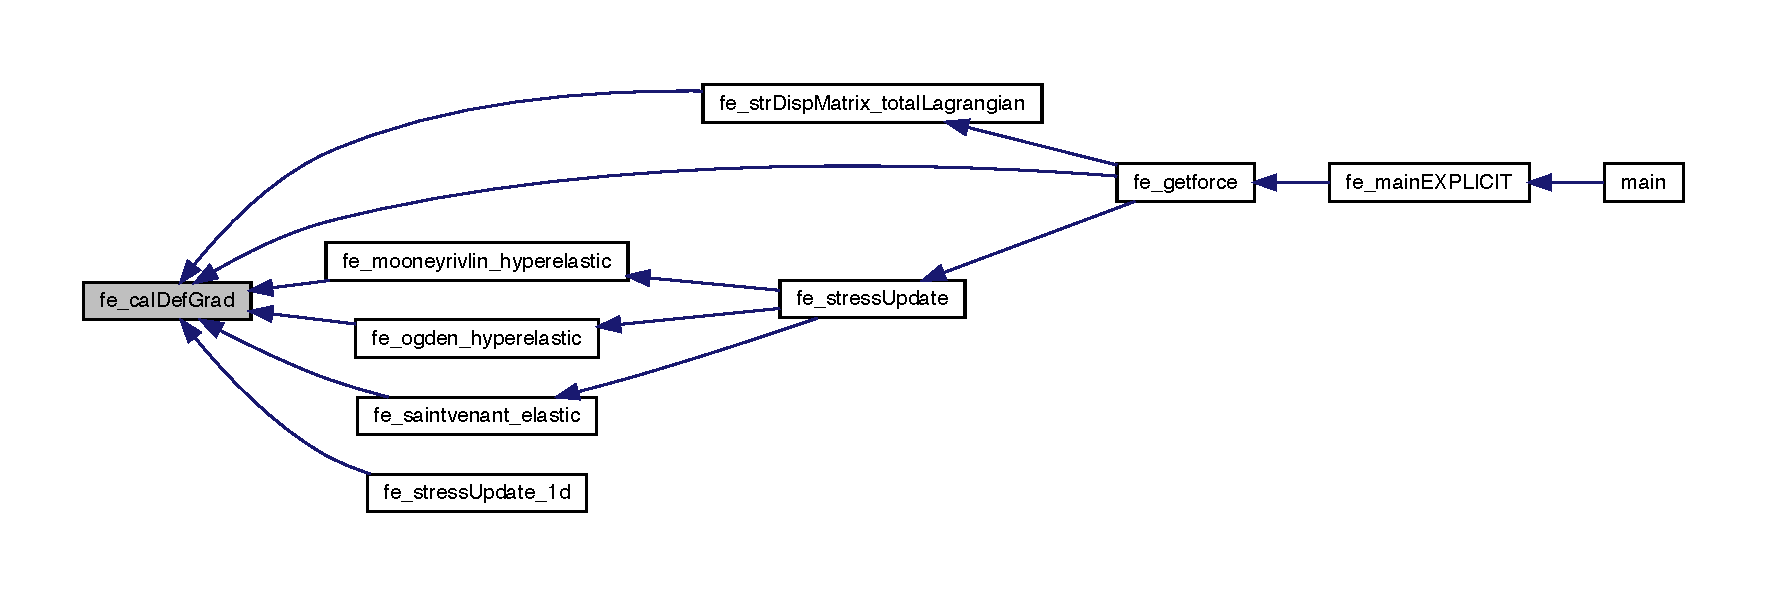
\includegraphics[width=350pt]{fe__cal_def_grad_8cpp_ae50379f74802347e04dbc022897f9cb0_icgraph}
\end{center}
\end{figure}

\hypertarget{fe__cal_jacobian_8cpp}{}\section{/\+Users/vsg111/\+Dropbox/\+Work/\+Papers/\+Paper\+\_\+\+E\+E\+M\+\_\+\+Computational/\+E\+E\+M\+\_\+\+Dynamic/source/\+F\+E\+M/\+Element\+Calculations/fe\+\_\+cal\+Jacobian.cpp File Reference}
\label{fe__cal_jacobian_8cpp}\index{/\+Users/vsg111/\+Dropbox/\+Work/\+Papers/\+Paper\+\_\+\+E\+E\+M\+\_\+\+Computational/\+E\+E\+M\+\_\+\+Dynamic/source/\+F\+E\+M/\+Element\+Calculations/fe\+\_\+cal\+Jacobian.\+cpp@{/\+Users/vsg111/\+Dropbox/\+Work/\+Papers/\+Paper\+\_\+\+E\+E\+M\+\_\+\+Computational/\+E\+E\+M\+\_\+\+Dynamic/source/\+F\+E\+M/\+Element\+Calculations/fe\+\_\+cal\+Jacobian.\+cpp}}
{\ttfamily \#include \char`\"{}functions.\+h\char`\"{}}\newline
\subsection*{Functions}
\begin{DoxyCompactItemize}
\item 
Matrix\+Xd \hyperlink{fe__cal_jacobian_8cpp_a12aa5a7a3443c6fcc5e65d3bcfc9bcc3}{fe\+\_\+cal\+Jacobian} (int dim, int nnel, Vector\+Xd dndr, Vector\+Xd dnds, Vector\+Xd dndt, double xcoord\mbox{[}$\,$\mbox{]}, double ycoord\mbox{[}$\,$\mbox{]}, double zcoord\mbox{[}$\,$\mbox{]})
\end{DoxyCompactItemize}


\subsection{Function Documentation}
\mbox{\Hypertarget{fe__cal_jacobian_8cpp_a12aa5a7a3443c6fcc5e65d3bcfc9bcc3}\label{fe__cal_jacobian_8cpp_a12aa5a7a3443c6fcc5e65d3bcfc9bcc3}} 
\index{fe\+\_\+cal\+Jacobian.\+cpp@{fe\+\_\+cal\+Jacobian.\+cpp}!fe\+\_\+cal\+Jacobian@{fe\+\_\+cal\+Jacobian}}
\index{fe\+\_\+cal\+Jacobian@{fe\+\_\+cal\+Jacobian}!fe\+\_\+cal\+Jacobian.\+cpp@{fe\+\_\+cal\+Jacobian.\+cpp}}
\subsubsection{\texorpdfstring{fe\+\_\+cal\+Jacobian()}{fe\_calJacobian()}}
{\footnotesize\ttfamily Matrix\+Xd fe\+\_\+cal\+Jacobian (\begin{DoxyParamCaption}\item[{int}]{dim,  }\item[{int}]{nnel,  }\item[{Vector\+Xd}]{dndr,  }\item[{Vector\+Xd}]{dnds,  }\item[{Vector\+Xd}]{dndt,  }\item[{double}]{xcoord\mbox{[}$\,$\mbox{]},  }\item[{double}]{ycoord\mbox{[}$\,$\mbox{]},  }\item[{double}]{zcoord\mbox{[}$\,$\mbox{]} }\end{DoxyParamCaption})}

Calculates the jacobian -- using the derivates of shape functions 

Definition at line 7 of file fe\+\_\+cal\+Jacobian.\+cpp.


\hypertarget{fe__cal_simp_transformation_8cpp}{}\section{source/\+Elements/\+Element\+Calculations/fe\+\_\+cal\+Simp\+Transformation.cpp File Reference}
\label{fe__cal_simp_transformation_8cpp}\index{source/\+Elements/\+Element\+Calculations/fe\+\_\+cal\+Simp\+Transformation.\+cpp@{source/\+Elements/\+Element\+Calculations/fe\+\_\+cal\+Simp\+Transformation.\+cpp}}
{\ttfamily \#include \char`\"{}functions.\+h\char`\"{}}\newline
Include dependency graph for fe\+\_\+cal\+Simp\+Transformation.\+cpp\+:
\nopagebreak
\begin{figure}[H]
\begin{center}
\leavevmode
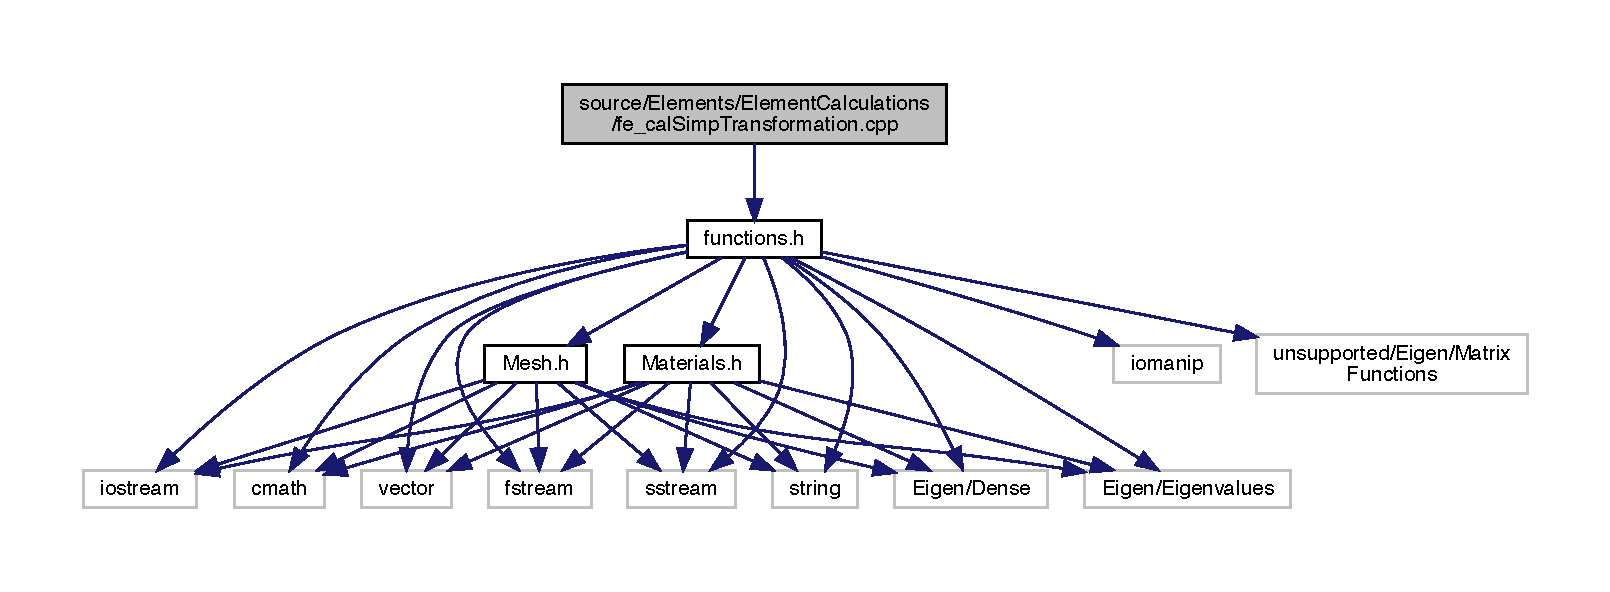
\includegraphics[width=350pt]{fe__cal_simp_transformation_8cpp__incl}
\end{center}
\end{figure}
\subsection*{Functions}
\begin{DoxyCompactItemize}
\item 
Matrix\+Xd \hyperlink{fe__cal_simp_transformation_8cpp_ae2eeba997bf4f0bc4749b92130de7ba3}{fe\+\_\+cal\+Simp\+Transformation} (Matrix\+Xd truss\+\_\+nodes)
\end{DoxyCompactItemize}


\subsection{Function Documentation}
\mbox{\Hypertarget{fe__cal_simp_transformation_8cpp_ae2eeba997bf4f0bc4749b92130de7ba3}\label{fe__cal_simp_transformation_8cpp_ae2eeba997bf4f0bc4749b92130de7ba3}} 
\index{fe\+\_\+cal\+Simp\+Transformation.\+cpp@{fe\+\_\+cal\+Simp\+Transformation.\+cpp}!fe\+\_\+cal\+Simp\+Transformation@{fe\+\_\+cal\+Simp\+Transformation}}
\index{fe\+\_\+cal\+Simp\+Transformation@{fe\+\_\+cal\+Simp\+Transformation}!fe\+\_\+cal\+Simp\+Transformation.\+cpp@{fe\+\_\+cal\+Simp\+Transformation.\+cpp}}
\subsubsection{\texorpdfstring{fe\+\_\+cal\+Simp\+Transformation()}{fe\_calSimpTransformation()}}
{\footnotesize\ttfamily Matrix\+Xd fe\+\_\+cal\+Simp\+Transformation (\begin{DoxyParamCaption}\item[{Matrix\+Xd}]{truss\+\_\+nodes }\end{DoxyParamCaption})}



Definition at line 7 of file fe\+\_\+cal\+Simp\+Transformation.\+cpp.

Here is the caller graph for this function\+:
\nopagebreak
\begin{figure}[H]
\begin{center}
\leavevmode
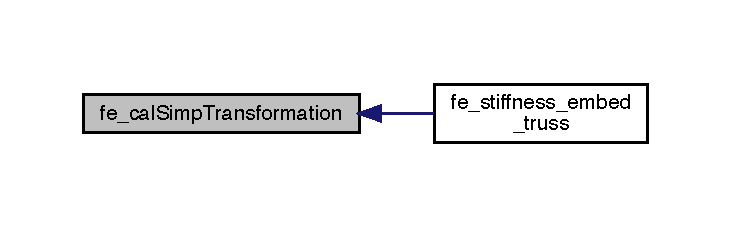
\includegraphics[width=350pt]{fe__cal_simp_transformation_8cpp_ae2eeba997bf4f0bc4749b92130de7ba3_icgraph}
\end{center}
\end{figure}

\hypertarget{fe__cal_transformation_8cpp}{}\section{source/\+Elements/\+Element\+Calculations/fe\+\_\+cal\+Transformation.cpp File Reference}
\label{fe__cal_transformation_8cpp}\index{source/\+Elements/\+Element\+Calculations/fe\+\_\+cal\+Transformation.\+cpp@{source/\+Elements/\+Element\+Calculations/fe\+\_\+cal\+Transformation.\+cpp}}
{\ttfamily \#include \char`\"{}functions.\+h\char`\"{}}\newline
Include dependency graph for fe\+\_\+cal\+Transformation.\+cpp\+:
\nopagebreak
\begin{figure}[H]
\begin{center}
\leavevmode
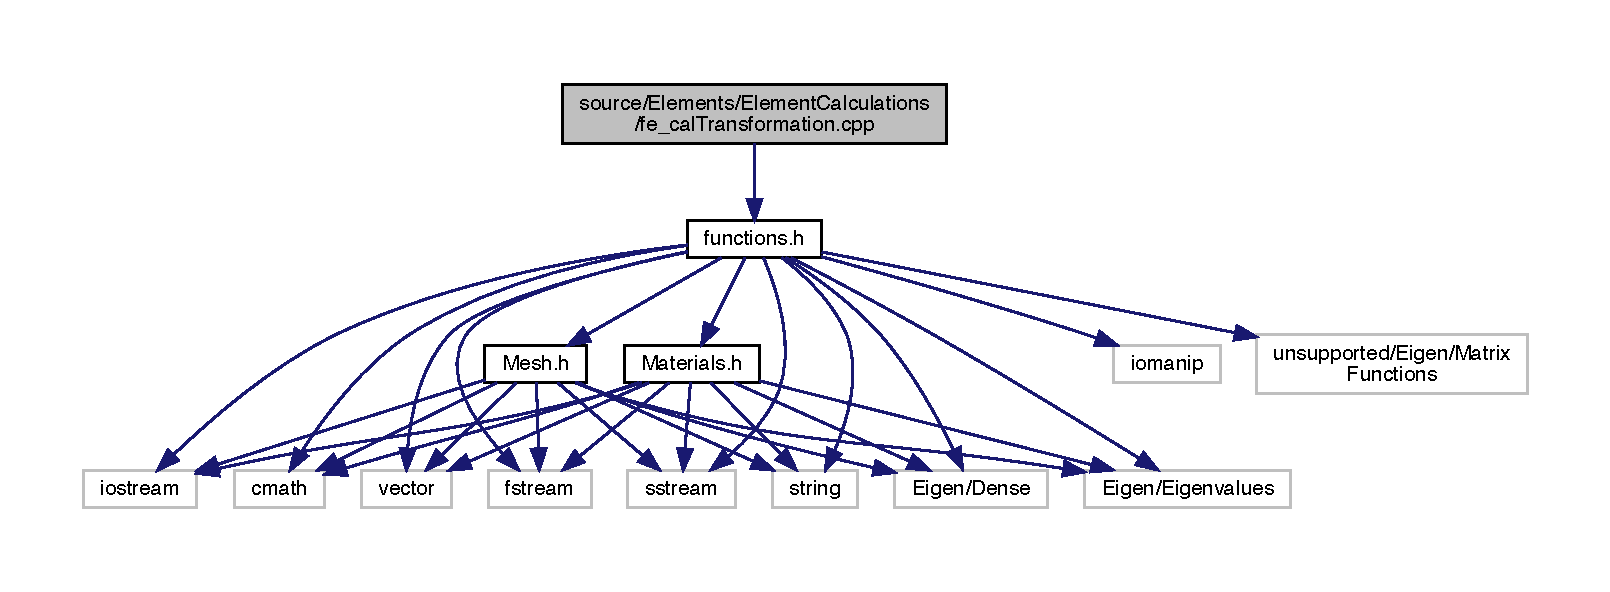
\includegraphics[width=350pt]{fe__cal_transformation_8cpp__incl}
\end{center}
\end{figure}
\subsection*{Functions}
\begin{DoxyCompactItemize}
\item 
Matrix\+Xd \hyperlink{fe__cal_transformation_8cpp_aa41c40dffea4251a07a8a3f5062f47ae}{fe\+\_\+cal\+Transformation} (Matrix\+Xd truss\+\_\+nodes, int choice)
\end{DoxyCompactItemize}


\subsection{Function Documentation}
\mbox{\Hypertarget{fe__cal_transformation_8cpp_aa41c40dffea4251a07a8a3f5062f47ae}\label{fe__cal_transformation_8cpp_aa41c40dffea4251a07a8a3f5062f47ae}} 
\index{fe\+\_\+cal\+Transformation.\+cpp@{fe\+\_\+cal\+Transformation.\+cpp}!fe\+\_\+cal\+Transformation@{fe\+\_\+cal\+Transformation}}
\index{fe\+\_\+cal\+Transformation@{fe\+\_\+cal\+Transformation}!fe\+\_\+cal\+Transformation.\+cpp@{fe\+\_\+cal\+Transformation.\+cpp}}
\subsubsection{\texorpdfstring{fe\+\_\+cal\+Transformation()}{fe\_calTransformation()}}
{\footnotesize\ttfamily Matrix\+Xd fe\+\_\+cal\+Transformation (\begin{DoxyParamCaption}\item[{Matrix\+Xd}]{truss\+\_\+nodes,  }\item[{int}]{choice }\end{DoxyParamCaption})}

Calculates the transformation matrix -\/ transformation from local (truss) coordinate system to global (3d hex) coordinate system 

Definition at line 7 of file fe\+\_\+cal\+Transformation.\+cpp.

Here is the caller graph for this function\+:
\nopagebreak
\begin{figure}[H]
\begin{center}
\leavevmode
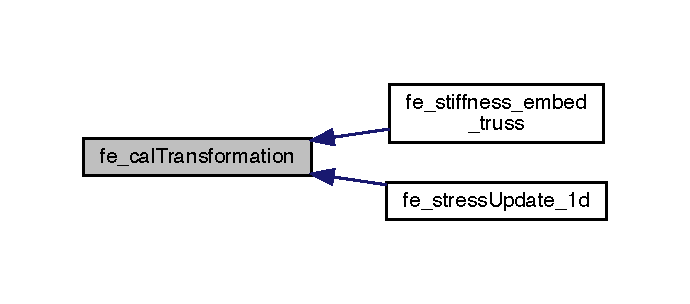
\includegraphics[width=331pt]{fe__cal_transformation_8cpp_aa41c40dffea4251a07a8a3f5062f47ae_icgraph}
\end{center}
\end{figure}

\hypertarget{fe__str_disp_matrix_8cpp}{}\section{source/\+Elements/\+Element\+Calculations/fe\+\_\+str\+Disp\+Matrix.cpp File Reference}
\label{fe__str_disp_matrix_8cpp}\index{source/\+Elements/\+Element\+Calculations/fe\+\_\+str\+Disp\+Matrix.\+cpp@{source/\+Elements/\+Element\+Calculations/fe\+\_\+str\+Disp\+Matrix.\+cpp}}
{\ttfamily \#include \char`\"{}functions.\+h\char`\"{}}\newline
Include dependency graph for fe\+\_\+str\+Disp\+Matrix.\+cpp\+:
\nopagebreak
\begin{figure}[H]
\begin{center}
\leavevmode
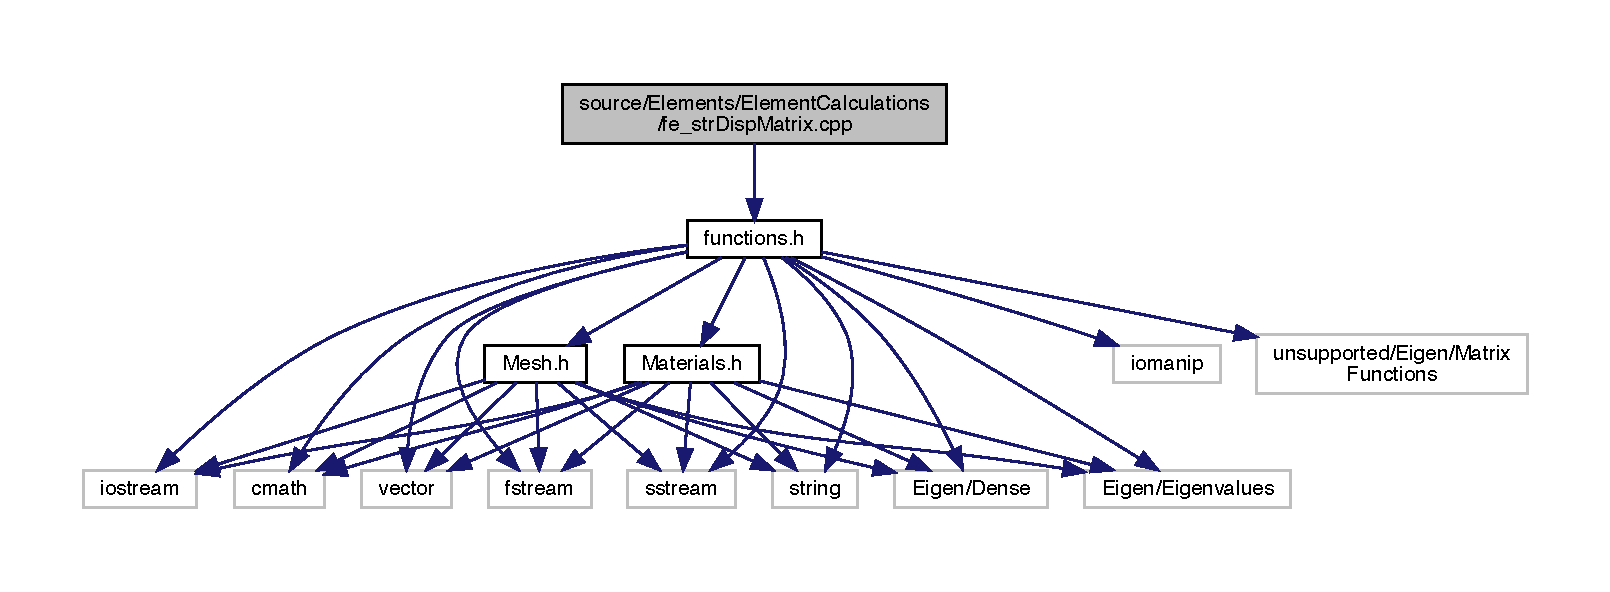
\includegraphics[width=350pt]{fe__str_disp_matrix_8cpp__incl}
\end{center}
\end{figure}
\subsection*{Functions}
\begin{DoxyCompactItemize}
\item 
Matrix\+Xd \hyperlink{fe__str_disp_matrix_8cpp_a4b49d2df4f86e7d0755971ab4bfa48b2}{fe\+\_\+str\+Disp\+Matrix} (int edof, int nnel, Vector\+Xd dndx, Vector\+Xd dndy, Vector\+Xd dndz)
\item 
Matrix\+Xd \hyperlink{fe__str_disp_matrix_8cpp_a8c9fd519c93c847cdf52de947964eb67}{fe\+\_\+str\+Disp\+Matrix\+\_\+total\+Lagrangian} (int edof, int nnel, Vector\+Xd dndx, Vector\+Xd dndy, Vector\+Xd dndz, Vector\+Xd u)
\end{DoxyCompactItemize}


\subsection{Function Documentation}
\mbox{\Hypertarget{fe__str_disp_matrix_8cpp_a4b49d2df4f86e7d0755971ab4bfa48b2}\label{fe__str_disp_matrix_8cpp_a4b49d2df4f86e7d0755971ab4bfa48b2}} 
\index{fe\+\_\+str\+Disp\+Matrix.\+cpp@{fe\+\_\+str\+Disp\+Matrix.\+cpp}!fe\+\_\+str\+Disp\+Matrix@{fe\+\_\+str\+Disp\+Matrix}}
\index{fe\+\_\+str\+Disp\+Matrix@{fe\+\_\+str\+Disp\+Matrix}!fe\+\_\+str\+Disp\+Matrix.\+cpp@{fe\+\_\+str\+Disp\+Matrix.\+cpp}}
\subsubsection{\texorpdfstring{fe\+\_\+str\+Disp\+Matrix()}{fe\_strDispMatrix()}}
{\footnotesize\ttfamily Matrix\+Xd fe\+\_\+str\+Disp\+Matrix (\begin{DoxyParamCaption}\item[{int}]{edof,  }\item[{int}]{nnel,  }\item[{Vector\+Xd}]{dndx,  }\item[{Vector\+Xd}]{dndy,  }\item[{Vector\+Xd}]{dndz }\end{DoxyParamCaption})}

Strain displacement matrix B 

Definition at line 5 of file fe\+\_\+str\+Disp\+Matrix.\+cpp.

Here is the caller graph for this function\+:
\nopagebreak
\begin{figure}[H]
\begin{center}
\leavevmode
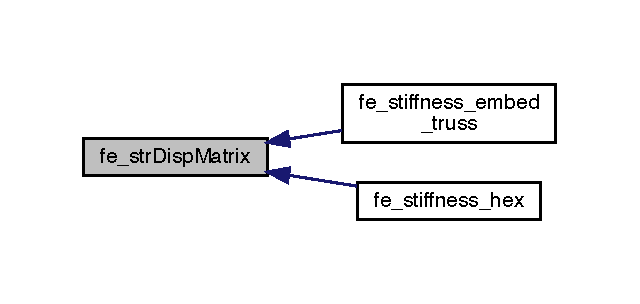
\includegraphics[width=307pt]{fe__str_disp_matrix_8cpp_a4b49d2df4f86e7d0755971ab4bfa48b2_icgraph}
\end{center}
\end{figure}
\mbox{\Hypertarget{fe__str_disp_matrix_8cpp_a8c9fd519c93c847cdf52de947964eb67}\label{fe__str_disp_matrix_8cpp_a8c9fd519c93c847cdf52de947964eb67}} 
\index{fe\+\_\+str\+Disp\+Matrix.\+cpp@{fe\+\_\+str\+Disp\+Matrix.\+cpp}!fe\+\_\+str\+Disp\+Matrix\+\_\+total\+Lagrangian@{fe\+\_\+str\+Disp\+Matrix\+\_\+total\+Lagrangian}}
\index{fe\+\_\+str\+Disp\+Matrix\+\_\+total\+Lagrangian@{fe\+\_\+str\+Disp\+Matrix\+\_\+total\+Lagrangian}!fe\+\_\+str\+Disp\+Matrix.\+cpp@{fe\+\_\+str\+Disp\+Matrix.\+cpp}}
\subsubsection{\texorpdfstring{fe\+\_\+str\+Disp\+Matrix\+\_\+total\+Lagrangian()}{fe\_strDispMatrix\_totalLagrangian()}}
{\footnotesize\ttfamily Matrix\+Xd fe\+\_\+str\+Disp\+Matrix\+\_\+total\+Lagrangian (\begin{DoxyParamCaption}\item[{int}]{edof,  }\item[{int}]{nnel,  }\item[{Vector\+Xd}]{dndx,  }\item[{Vector\+Xd}]{dndy,  }\item[{Vector\+Xd}]{dndz,  }\item[{Vector\+Xd}]{u }\end{DoxyParamCaption})}

Calculates the strain displacement matrix in total lagrangian system 

Definition at line 31 of file fe\+\_\+str\+Disp\+Matrix.\+cpp.

Here is the call graph for this function\+:
\nopagebreak
\begin{figure}[H]
\begin{center}
\leavevmode
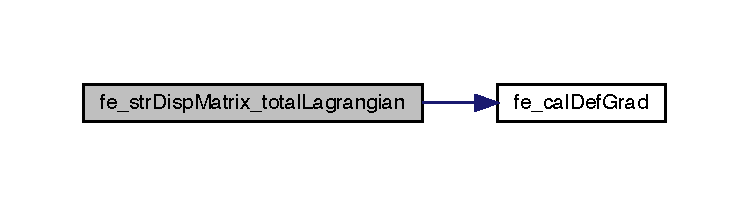
\includegraphics[width=350pt]{fe__str_disp_matrix_8cpp_a8c9fd519c93c847cdf52de947964eb67_cgraph}
\end{center}
\end{figure}
Here is the caller graph for this function\+:
\nopagebreak
\begin{figure}[H]
\begin{center}
\leavevmode
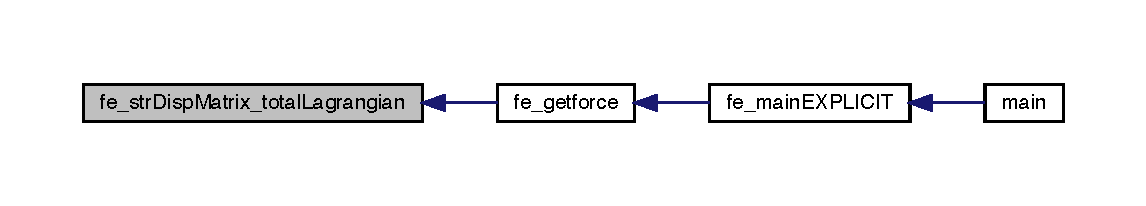
\includegraphics[width=350pt]{fe__str_disp_matrix_8cpp_a8c9fd519c93c847cdf52de947964eb67_icgraph}
\end{center}
\end{figure}

\hypertarget{fe__tensor2voigt_8cpp}{}\section{source/\+Elements/\+Element\+Calculations/fe\+\_\+tensor2voigt.cpp File Reference}
\label{fe__tensor2voigt_8cpp}\index{source/\+Elements/\+Element\+Calculations/fe\+\_\+tensor2voigt.\+cpp@{source/\+Elements/\+Element\+Calculations/fe\+\_\+tensor2voigt.\+cpp}}
{\ttfamily \#include \char`\"{}functions.\+h\char`\"{}}\newline
Include dependency graph for fe\+\_\+tensor2voigt.\+cpp\+:
\nopagebreak
\begin{figure}[H]
\begin{center}
\leavevmode
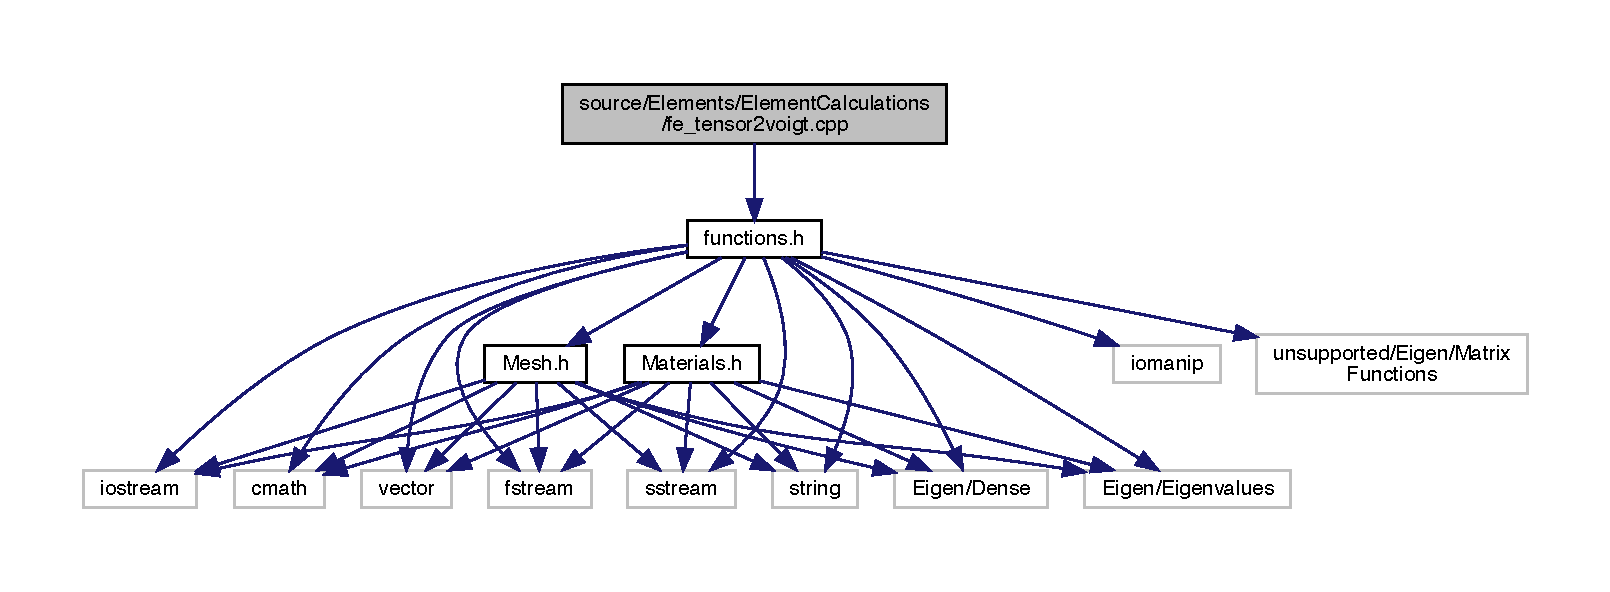
\includegraphics[width=350pt]{fe__tensor2voigt_8cpp__incl}
\end{center}
\end{figure}
\subsection*{Functions}
\begin{DoxyCompactItemize}
\item 
Vector\+Xd \hyperlink{fe__tensor2voigt_8cpp_a73c4523ec7068af2af9e8431021f5fdf}{fe\+\_\+tensor2voigt} (Matrix\+Xd A)
\end{DoxyCompactItemize}


\subsection{Function Documentation}
\mbox{\Hypertarget{fe__tensor2voigt_8cpp_a73c4523ec7068af2af9e8431021f5fdf}\label{fe__tensor2voigt_8cpp_a73c4523ec7068af2af9e8431021f5fdf}} 
\index{fe\+\_\+tensor2voigt.\+cpp@{fe\+\_\+tensor2voigt.\+cpp}!fe\+\_\+tensor2voigt@{fe\+\_\+tensor2voigt}}
\index{fe\+\_\+tensor2voigt@{fe\+\_\+tensor2voigt}!fe\+\_\+tensor2voigt.\+cpp@{fe\+\_\+tensor2voigt.\+cpp}}
\subsubsection{\texorpdfstring{fe\+\_\+tensor2voigt()}{fe\_tensor2voigt()}}
{\footnotesize\ttfamily Vector\+Xd fe\+\_\+tensor2voigt (\begin{DoxyParamCaption}\item[{Matrix\+Xd}]{A }\end{DoxyParamCaption})}

This function converts tensor into voigt\textquotesingle{}s vector notation The tensor should be either 2\+X2 or 3\+X3. The tensor should be symmetric for its transformation into Voigt Vector 

Definition at line 8 of file fe\+\_\+tensor2voigt.\+cpp.

Here is the caller graph for this function\+:
\nopagebreak
\begin{figure}[H]
\begin{center}
\leavevmode
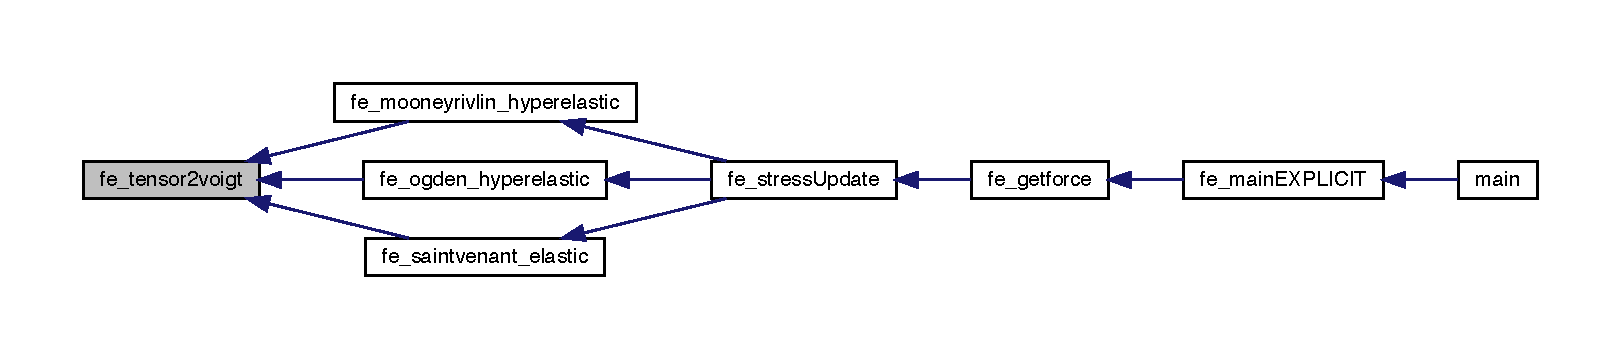
\includegraphics[width=350pt]{fe__tensor2voigt_8cpp_a73c4523ec7068af2af9e8431021f5fdf_icgraph}
\end{center}
\end{figure}

\hypertarget{fe__transform_mass_8cpp}{}\section{source/\+Elements/\+Element\+Calculations/fe\+\_\+transform\+Mass.cpp File Reference}
\label{fe__transform_mass_8cpp}\index{source/\+Elements/\+Element\+Calculations/fe\+\_\+transform\+Mass.\+cpp@{source/\+Elements/\+Element\+Calculations/fe\+\_\+transform\+Mass.\+cpp}}
{\ttfamily \#include $<$iostream$>$}\newline
{\ttfamily \#include \char`\"{}functions.\+h\char`\"{}}\newline
Include dependency graph for fe\+\_\+transform\+Mass.\+cpp\+:
\nopagebreak
\begin{figure}[H]
\begin{center}
\leavevmode
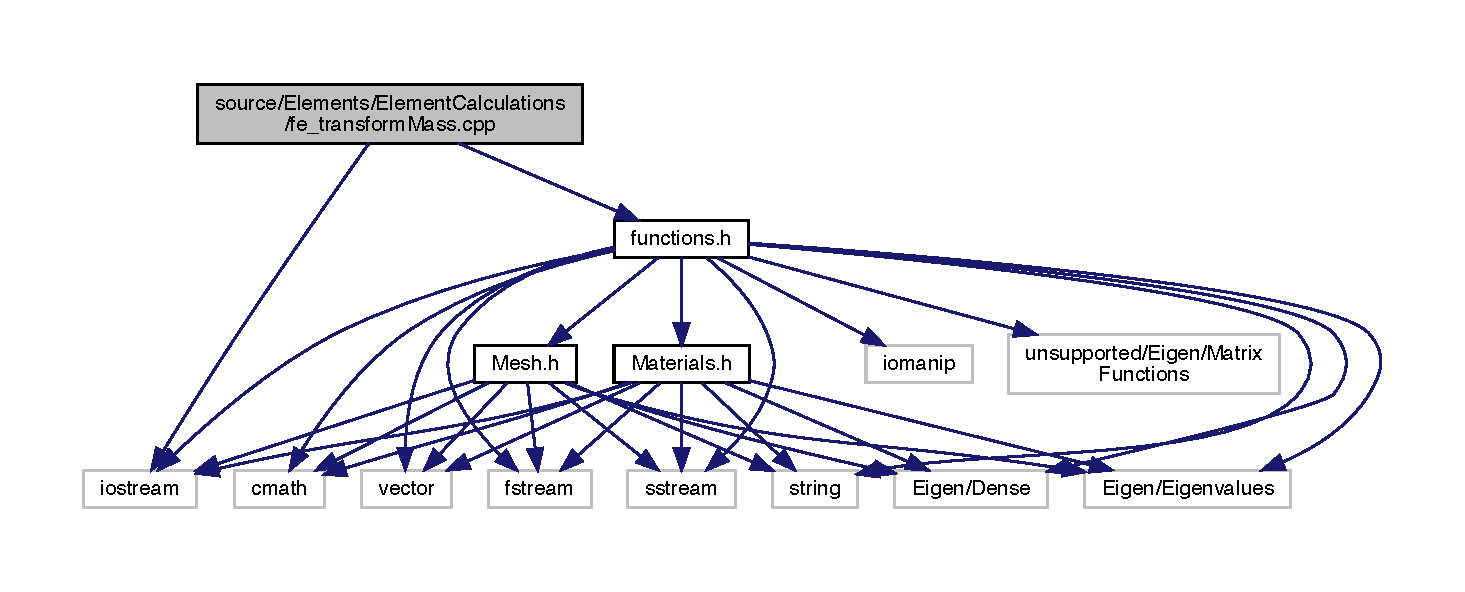
\includegraphics[width=350pt]{fe__transform_mass_8cpp__incl}
\end{center}
\end{figure}
\subsection*{Functions}
\begin{DoxyCompactItemize}
\item 
Matrix\+Xd \hyperlink{fe__transform_mass_8cpp_ab747d046148af042245ed13ca720c5ec}{fe\+\_\+transform\+Mass} (Matrix\+Xd m, int opt)
\end{DoxyCompactItemize}


\subsection{Function Documentation}
\mbox{\Hypertarget{fe__transform_mass_8cpp_ab747d046148af042245ed13ca720c5ec}\label{fe__transform_mass_8cpp_ab747d046148af042245ed13ca720c5ec}} 
\index{fe\+\_\+transform\+Mass.\+cpp@{fe\+\_\+transform\+Mass.\+cpp}!fe\+\_\+transform\+Mass@{fe\+\_\+transform\+Mass}}
\index{fe\+\_\+transform\+Mass@{fe\+\_\+transform\+Mass}!fe\+\_\+transform\+Mass.\+cpp@{fe\+\_\+transform\+Mass.\+cpp}}
\subsubsection{\texorpdfstring{fe\+\_\+transform\+Mass()}{fe\_transformMass()}}
{\footnotesize\ttfamily Matrix\+Xd fe\+\_\+transform\+Mass (\begin{DoxyParamCaption}\item[{Matrix\+Xd}]{m,  }\item[{int}]{opt }\end{DoxyParamCaption})}

Converts a normal mass matrix into a lumped mass matrix 

Definition at line 6 of file fe\+\_\+transform\+Mass.\+cpp.

Here is the caller graph for this function\+:
\nopagebreak
\begin{figure}[H]
\begin{center}
\leavevmode
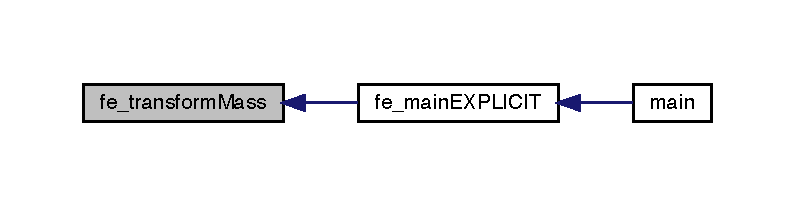
\includegraphics[width=350pt]{fe__transform_mass_8cpp_ab747d046148af042245ed13ca720c5ec_icgraph}
\end{center}
\end{figure}

\hypertarget{fe__voigt2tensor_8cpp}{}\section{source/\+Elements/\+Element\+Calculations/fe\+\_\+voigt2tensor.cpp File Reference}
\label{fe__voigt2tensor_8cpp}\index{source/\+Elements/\+Element\+Calculations/fe\+\_\+voigt2tensor.\+cpp@{source/\+Elements/\+Element\+Calculations/fe\+\_\+voigt2tensor.\+cpp}}
{\ttfamily \#include \char`\"{}functions.\+h\char`\"{}}\newline
Include dependency graph for fe\+\_\+voigt2tensor.\+cpp\+:
\nopagebreak
\begin{figure}[H]
\begin{center}
\leavevmode
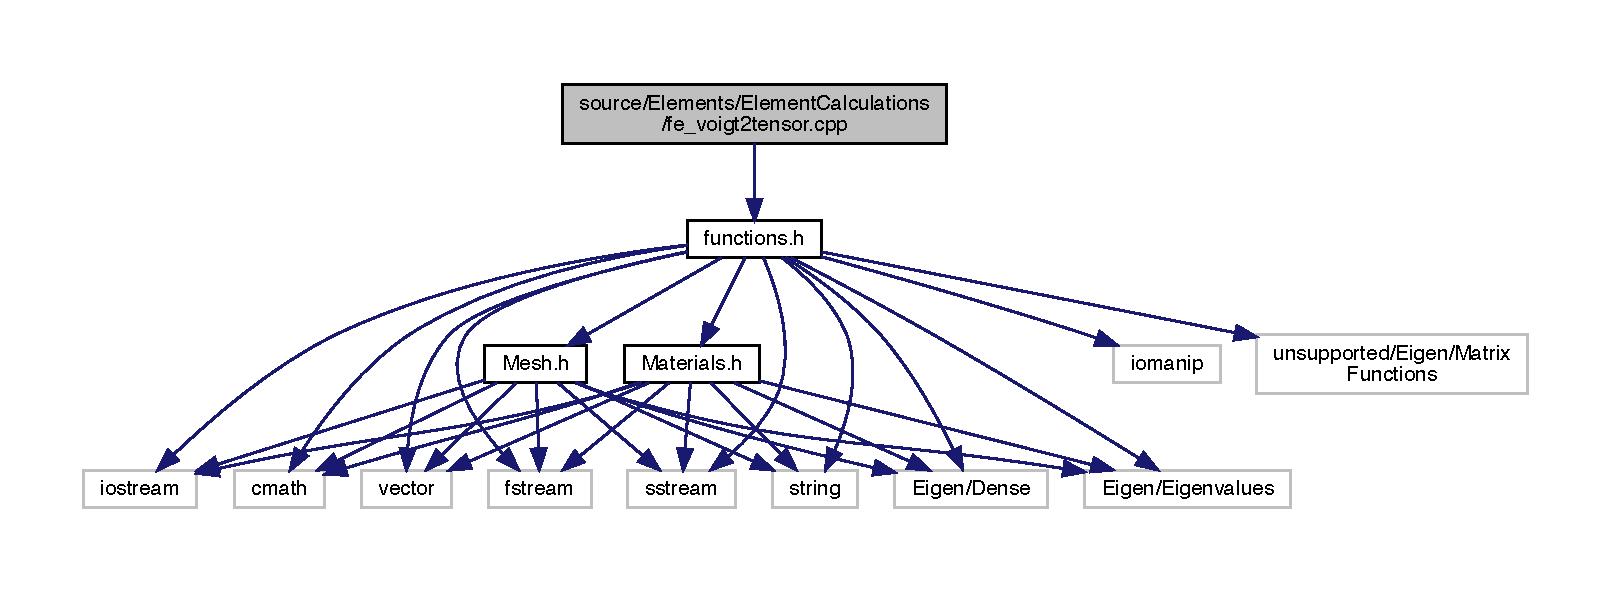
\includegraphics[width=350pt]{fe__voigt2tensor_8cpp__incl}
\end{center}
\end{figure}
\subsection*{Functions}
\begin{DoxyCompactItemize}
\item 
Matrix\+Xd \hyperlink{fe__voigt2tensor_8cpp_a721a169d6a3d34b5584817ccd1c48cd7}{fe\+\_\+voigt2tensor} (Vector\+Xd B)
\end{DoxyCompactItemize}


\subsection{Function Documentation}
\mbox{\Hypertarget{fe__voigt2tensor_8cpp_a721a169d6a3d34b5584817ccd1c48cd7}\label{fe__voigt2tensor_8cpp_a721a169d6a3d34b5584817ccd1c48cd7}} 
\index{fe\+\_\+voigt2tensor.\+cpp@{fe\+\_\+voigt2tensor.\+cpp}!fe\+\_\+voigt2tensor@{fe\+\_\+voigt2tensor}}
\index{fe\+\_\+voigt2tensor@{fe\+\_\+voigt2tensor}!fe\+\_\+voigt2tensor.\+cpp@{fe\+\_\+voigt2tensor.\+cpp}}
\subsubsection{\texorpdfstring{fe\+\_\+voigt2tensor()}{fe\_voigt2tensor()}}
{\footnotesize\ttfamily Matrix\+Xd fe\+\_\+voigt2tensor (\begin{DoxyParamCaption}\item[{Vector\+Xd}]{B }\end{DoxyParamCaption})}

This function converts vector in voigt\textquotesingle{}s vector notation into a tensor The tensor will be either 2\+X2 or 3\+X3. 

Definition at line 8 of file fe\+\_\+voigt2tensor.\+cpp.


\hypertarget{fe__stiffness__embed__truss_8cpp}{}\section{source/\+Elements/\+Internal\+Nodal\+Force/fe\+\_\+stiffness\+\_\+embed\+\_\+truss.cpp File Reference}
\label{fe__stiffness__embed__truss_8cpp}\index{source/\+Elements/\+Internal\+Nodal\+Force/fe\+\_\+stiffness\+\_\+embed\+\_\+truss.\+cpp@{source/\+Elements/\+Internal\+Nodal\+Force/fe\+\_\+stiffness\+\_\+embed\+\_\+truss.\+cpp}}
{\ttfamily \#include \char`\"{}functions.\+h\char`\"{}}\newline
Include dependency graph for fe\+\_\+stiffness\+\_\+embed\+\_\+truss.\+cpp\+:
\nopagebreak
\begin{figure}[H]
\begin{center}
\leavevmode
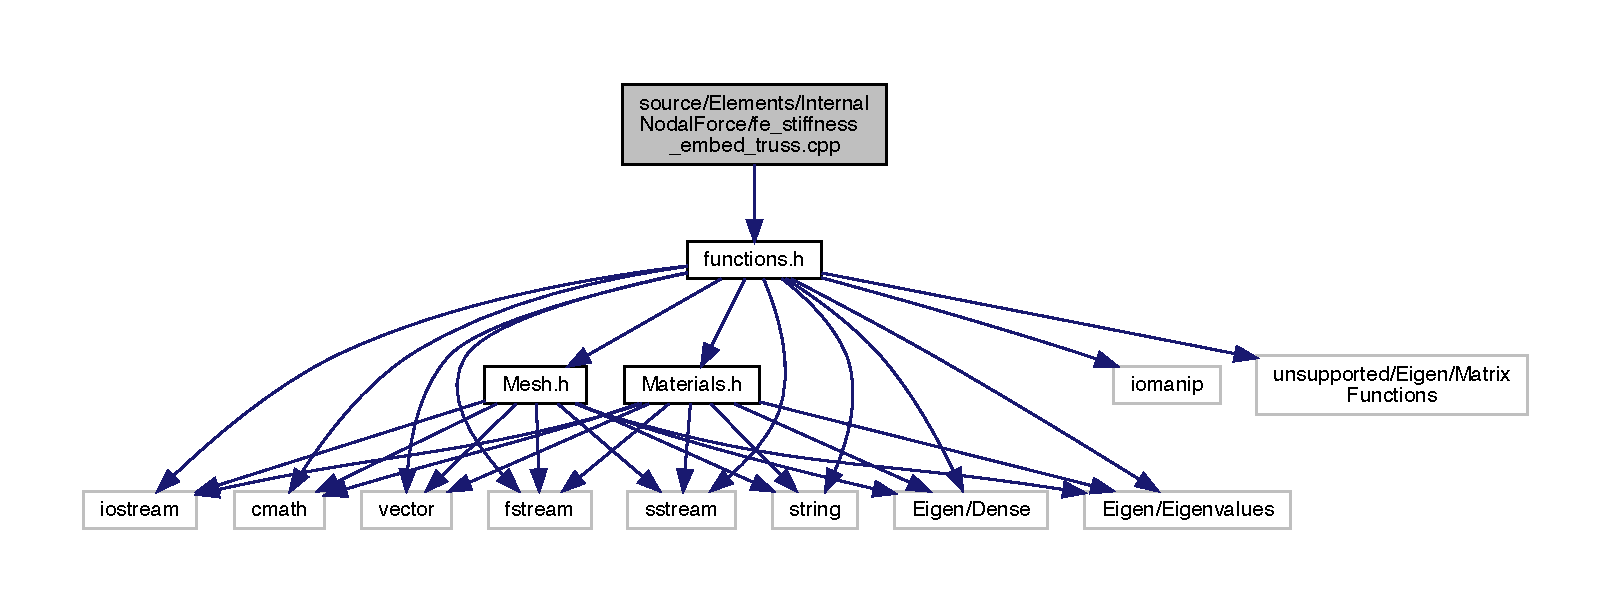
\includegraphics[width=350pt]{fe__stiffness__embed__truss_8cpp__incl}
\end{center}
\end{figure}
\subsection*{Functions}
\begin{DoxyCompactItemize}
\item 
Matrix\+Xd \hyperlink{fe__stiffness__embed__truss_8cpp_ab3798340a27f0972299b3820aab0ccba}{fe\+\_\+stiffness\+\_\+embed\+\_\+truss} (Matrix\+Xd nodes\+\_\+truss, Matrix\+Xd elements\+\_\+truss, double E\+\_\+truss, double \hyperlink{main_8cpp_a2f98cf28208251affb988effe3a89708}{A\+\_\+truss}, int \hyperlink{main_8cpp_aa789fe4d8a13fd0990b630909430d5d0}{ndof}, int nnel, int edof, double xcoord\mbox{[}$\,$\mbox{]}, double ycoord\mbox{[}$\,$\mbox{]}, double zcoord\mbox{[}$\,$\mbox{]})
\end{DoxyCompactItemize}


\subsection{Function Documentation}
\mbox{\Hypertarget{fe__stiffness__embed__truss_8cpp_ab3798340a27f0972299b3820aab0ccba}\label{fe__stiffness__embed__truss_8cpp_ab3798340a27f0972299b3820aab0ccba}} 
\index{fe\+\_\+stiffness\+\_\+embed\+\_\+truss.\+cpp@{fe\+\_\+stiffness\+\_\+embed\+\_\+truss.\+cpp}!fe\+\_\+stiffness\+\_\+embed\+\_\+truss@{fe\+\_\+stiffness\+\_\+embed\+\_\+truss}}
\index{fe\+\_\+stiffness\+\_\+embed\+\_\+truss@{fe\+\_\+stiffness\+\_\+embed\+\_\+truss}!fe\+\_\+stiffness\+\_\+embed\+\_\+truss.\+cpp@{fe\+\_\+stiffness\+\_\+embed\+\_\+truss.\+cpp}}
\subsubsection{\texorpdfstring{fe\+\_\+stiffness\+\_\+embed\+\_\+truss()}{fe\_stiffness\_embed\_truss()}}
{\footnotesize\ttfamily Matrix\+Xd fe\+\_\+stiffness\+\_\+embed\+\_\+truss (\begin{DoxyParamCaption}\item[{Matrix\+Xd}]{nodes\+\_\+truss,  }\item[{Matrix\+Xd}]{elements\+\_\+truss,  }\item[{double}]{E\+\_\+truss,  }\item[{double}]{A\+\_\+truss,  }\item[{int}]{ndof,  }\item[{int}]{nnel,  }\item[{int}]{edof,  }\item[{double}]{xcoord\mbox{[}$\,$\mbox{]},  }\item[{double}]{ycoord\mbox{[}$\,$\mbox{]},  }\item[{double}]{zcoord\mbox{[}$\,$\mbox{]} }\end{DoxyParamCaption})}

Internal nodal force vector for a truss (1D) element 

Definition at line 6 of file fe\+\_\+stiffness\+\_\+embed\+\_\+truss.\+cpp.

Here is the call graph for this function\+:
\nopagebreak
\begin{figure}[H]
\begin{center}
\leavevmode
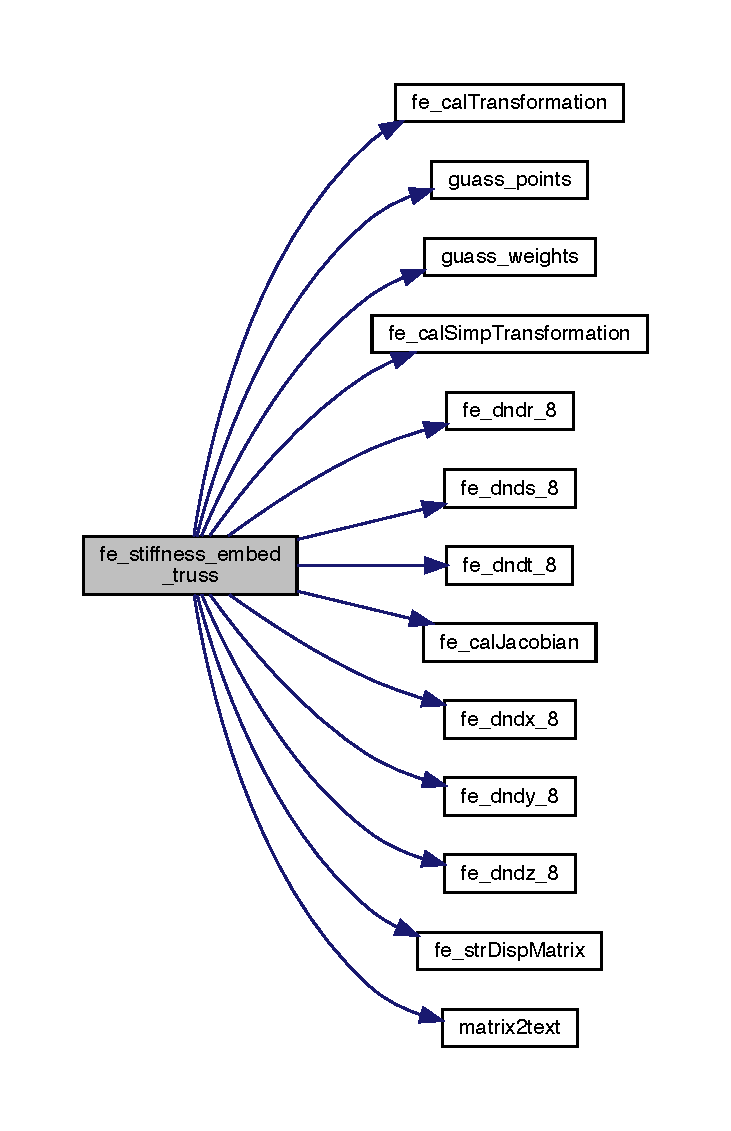
\includegraphics[width=350pt]{fe__stiffness__embed__truss_8cpp_ab3798340a27f0972299b3820aab0ccba_cgraph}
\end{center}
\end{figure}

\hypertarget{fe__stiffness__hex_8cpp}{}\section{source/\+Elements/\+Internal\+Nodal\+Force/fe\+\_\+stiffness\+\_\+hex.cpp File Reference}
\label{fe__stiffness__hex_8cpp}\index{source/\+Elements/\+Internal\+Nodal\+Force/fe\+\_\+stiffness\+\_\+hex.\+cpp@{source/\+Elements/\+Internal\+Nodal\+Force/fe\+\_\+stiffness\+\_\+hex.\+cpp}}
{\ttfamily \#include \char`\"{}functions.\+h\char`\"{}}\newline
Include dependency graph for fe\+\_\+stiffness\+\_\+hex.\+cpp\+:
\nopagebreak
\begin{figure}[H]
\begin{center}
\leavevmode
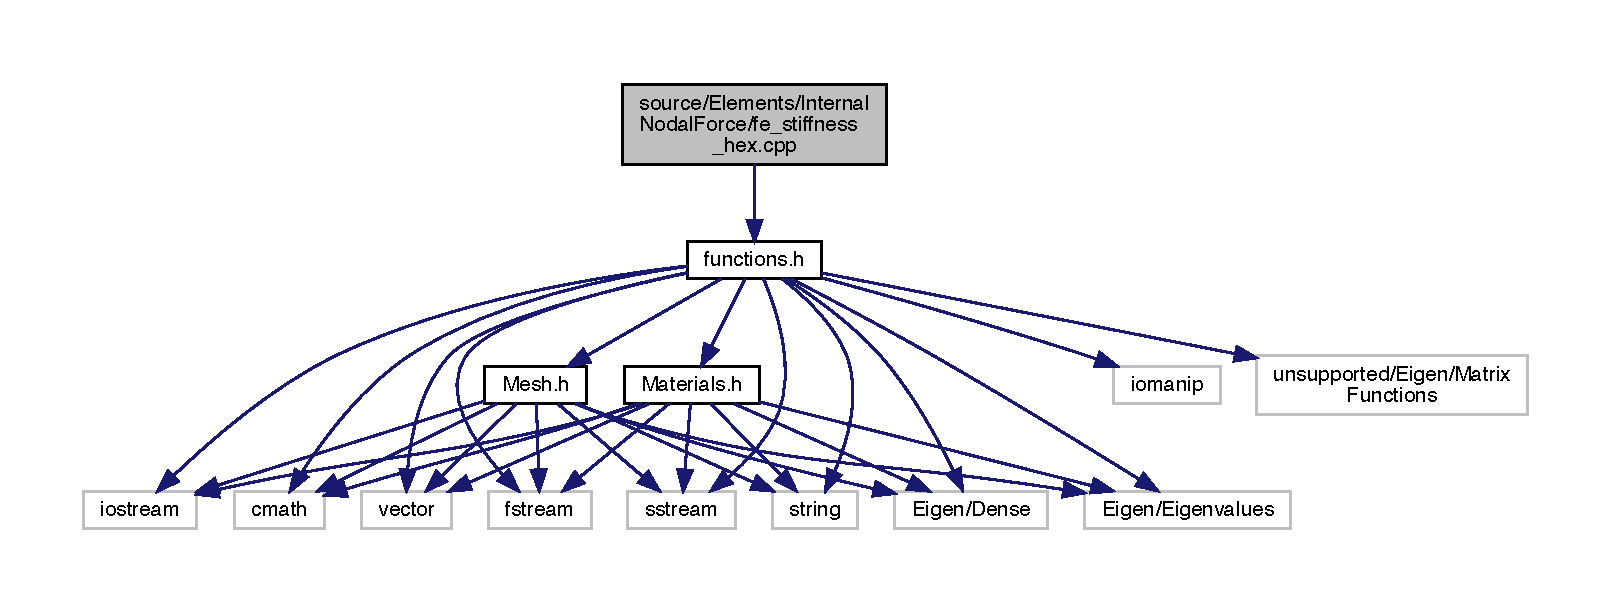
\includegraphics[width=350pt]{fe__stiffness__hex_8cpp__incl}
\end{center}
\end{figure}
\subsection*{Functions}
\begin{DoxyCompactItemize}
\item 
Matrix\+Xd \hyperlink{fe__stiffness__hex_8cpp_a9378d4fc517465015411134456235a76}{fe\+\_\+stiffness\+\_\+hex} (double E, double nu, int \hyperlink{main_8cpp_aa789fe4d8a13fd0990b630909430d5d0}{ndof}, int nnel, int edof, double xcoord\mbox{[}$\,$\mbox{]}, double ycoord\mbox{[}$\,$\mbox{]}, double zcoord\mbox{[}$\,$\mbox{]})
\end{DoxyCompactItemize}


\subsection{Function Documentation}
\mbox{\Hypertarget{fe__stiffness__hex_8cpp_a9378d4fc517465015411134456235a76}\label{fe__stiffness__hex_8cpp_a9378d4fc517465015411134456235a76}} 
\index{fe\+\_\+stiffness\+\_\+hex.\+cpp@{fe\+\_\+stiffness\+\_\+hex.\+cpp}!fe\+\_\+stiffness\+\_\+hex@{fe\+\_\+stiffness\+\_\+hex}}
\index{fe\+\_\+stiffness\+\_\+hex@{fe\+\_\+stiffness\+\_\+hex}!fe\+\_\+stiffness\+\_\+hex.\+cpp@{fe\+\_\+stiffness\+\_\+hex.\+cpp}}
\subsubsection{\texorpdfstring{fe\+\_\+stiffness\+\_\+hex()}{fe\_stiffness\_hex()}}
{\footnotesize\ttfamily Matrix\+Xd fe\+\_\+stiffness\+\_\+hex (\begin{DoxyParamCaption}\item[{double}]{E,  }\item[{double}]{nu,  }\item[{int}]{ndof,  }\item[{int}]{nnel,  }\item[{int}]{edof,  }\item[{double}]{xcoord\mbox{[}$\,$\mbox{]},  }\item[{double}]{ycoord\mbox{[}$\,$\mbox{]},  }\item[{double}]{zcoord\mbox{[}$\,$\mbox{]} }\end{DoxyParamCaption})}

Internal nodal force vector for a hexahedral element 

Definition at line 7 of file fe\+\_\+stiffness\+\_\+hex.\+cpp.

Here is the call graph for this function\+:
\nopagebreak
\begin{figure}[H]
\begin{center}
\leavevmode
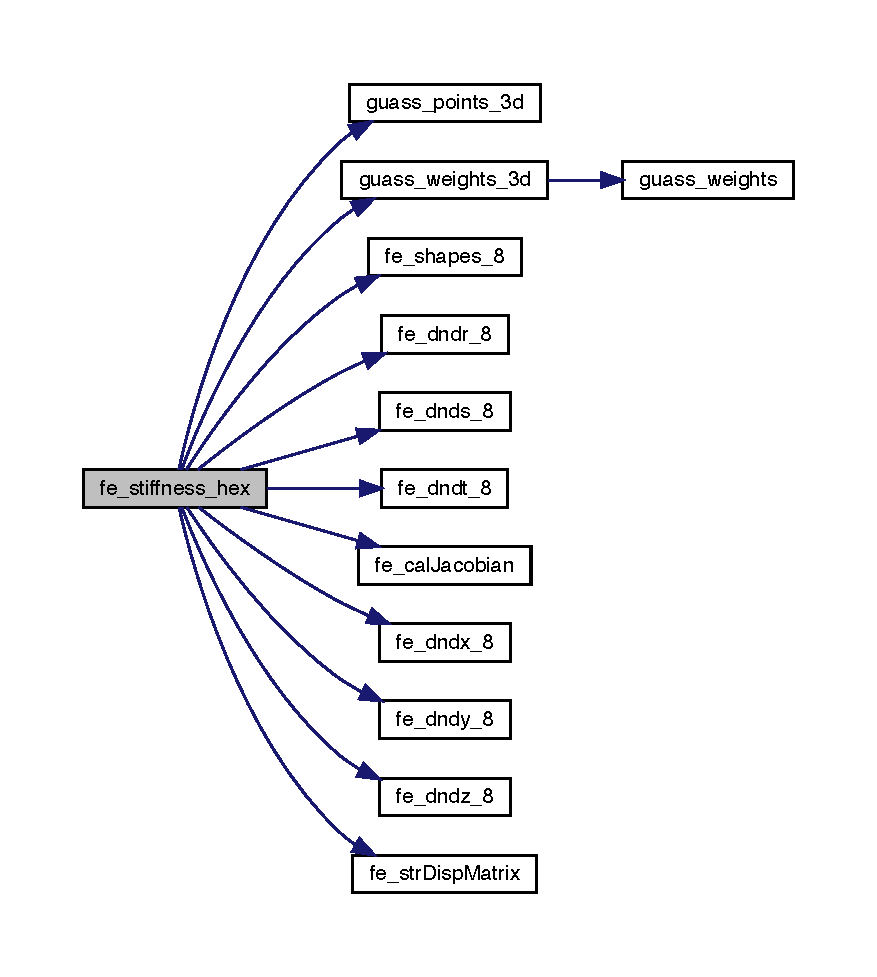
\includegraphics[width=350pt]{fe__stiffness__hex_8cpp_a9378d4fc517465015411134456235a76_cgraph}
\end{center}
\end{figure}

\hypertarget{fe__mass__hex_8cpp}{}\section{/\+Users/vsg111/\+Dropbox/\+Work/\+Papers/\+Paper\+\_\+\+E\+E\+M\+\_\+\+Computational/\+E\+E\+M\+\_\+\+Dynamic/source/\+Elements/\+Mass/fe\+\_\+mass\+\_\+hex.cpp File Reference}
\label{fe__mass__hex_8cpp}\index{/\+Users/vsg111/\+Dropbox/\+Work/\+Papers/\+Paper\+\_\+\+E\+E\+M\+\_\+\+Computational/\+E\+E\+M\+\_\+\+Dynamic/source/\+Elements/\+Mass/fe\+\_\+mass\+\_\+hex.\+cpp@{/\+Users/vsg111/\+Dropbox/\+Work/\+Papers/\+Paper\+\_\+\+E\+E\+M\+\_\+\+Computational/\+E\+E\+M\+\_\+\+Dynamic/source/\+Elements/\+Mass/fe\+\_\+mass\+\_\+hex.\+cpp}}
{\ttfamily \#include \char`\"{}functions.\+h\char`\"{}}\newline
\subsection*{Functions}
\begin{DoxyCompactItemize}
\item 
Matrix\+Xd \hyperlink{fe__mass__hex_8cpp_a04906e61b8cfdc7232924a594b95eb1f}{fe\+\_\+mass\+\_\+hex} (double rho, int \hyperlink{main_8cpp_aa789fe4d8a13fd0990b630909430d5d0}{ndof}, int nnel, int edof, double xcoord\mbox{[}$\,$\mbox{]}, double ycoord\mbox{[}$\,$\mbox{]}, double zcoord\mbox{[}$\,$\mbox{]})
\item 
Matrix\+Xd \hyperlink{fe__mass__hex_8cpp_a350d27ea0f1de929495d659b26f428d2}{fe\+\_\+mass\+\_\+truss} (double rho, double \hyperlink{main_8cpp_a2f98cf28208251affb988effe3a89708}{A\+\_\+truss}, int edof, Matrix\+Xd nodes, Matrix\+Xd elements)
\end{DoxyCompactItemize}


\subsection{Function Documentation}
\mbox{\Hypertarget{fe__mass__hex_8cpp_a04906e61b8cfdc7232924a594b95eb1f}\label{fe__mass__hex_8cpp_a04906e61b8cfdc7232924a594b95eb1f}} 
\index{fe\+\_\+mass\+\_\+hex.\+cpp@{fe\+\_\+mass\+\_\+hex.\+cpp}!fe\+\_\+mass\+\_\+hex@{fe\+\_\+mass\+\_\+hex}}
\index{fe\+\_\+mass\+\_\+hex@{fe\+\_\+mass\+\_\+hex}!fe\+\_\+mass\+\_\+hex.\+cpp@{fe\+\_\+mass\+\_\+hex.\+cpp}}
\subsubsection{\texorpdfstring{fe\+\_\+mass\+\_\+hex()}{fe\_mass\_hex()}}
{\footnotesize\ttfamily Matrix\+Xd fe\+\_\+mass\+\_\+hex (\begin{DoxyParamCaption}\item[{double}]{rho,  }\item[{int}]{ndof,  }\item[{int}]{nnel,  }\item[{int}]{edof,  }\item[{double}]{xcoord\mbox{[}$\,$\mbox{]},  }\item[{double}]{ycoord\mbox{[}$\,$\mbox{]},  }\item[{double}]{zcoord\mbox{[}$\,$\mbox{]} }\end{DoxyParamCaption})}

Calculates the mass matrix for a hex element 

Definition at line 7 of file fe\+\_\+mass\+\_\+hex.\+cpp.

\mbox{\Hypertarget{fe__mass__hex_8cpp_a350d27ea0f1de929495d659b26f428d2}\label{fe__mass__hex_8cpp_a350d27ea0f1de929495d659b26f428d2}} 
\index{fe\+\_\+mass\+\_\+hex.\+cpp@{fe\+\_\+mass\+\_\+hex.\+cpp}!fe\+\_\+mass\+\_\+truss@{fe\+\_\+mass\+\_\+truss}}
\index{fe\+\_\+mass\+\_\+truss@{fe\+\_\+mass\+\_\+truss}!fe\+\_\+mass\+\_\+hex.\+cpp@{fe\+\_\+mass\+\_\+hex.\+cpp}}
\subsubsection{\texorpdfstring{fe\+\_\+mass\+\_\+truss()}{fe\_mass\_truss()}}
{\footnotesize\ttfamily Matrix\+Xd fe\+\_\+mass\+\_\+truss (\begin{DoxyParamCaption}\item[{double}]{rho,  }\item[{double}]{A\+\_\+truss,  }\item[{int}]{edof,  }\item[{Matrix\+Xd}]{nodes,  }\item[{Matrix\+Xd}]{elements }\end{DoxyParamCaption})}

Calculates the mass of a truss element 

Definition at line 81 of file fe\+\_\+mass\+\_\+hex.\+cpp.


\hypertarget{fe__guass__points_8cpp}{}\section{/\+Users/vsg111/\+Dropbox/\+Work/\+Papers/\+Paper\+\_\+\+E\+E\+M\+\_\+\+Computational/\+E\+E\+M\+\_\+\+Dynamic/source/\+Elements/\+Quadrature/fe\+\_\+guass\+\_\+points.cpp File Reference}
\label{fe__guass__points_8cpp}\index{/\+Users/vsg111/\+Dropbox/\+Work/\+Papers/\+Paper\+\_\+\+E\+E\+M\+\_\+\+Computational/\+E\+E\+M\+\_\+\+Dynamic/source/\+Elements/\+Quadrature/fe\+\_\+guass\+\_\+points.\+cpp@{/\+Users/vsg111/\+Dropbox/\+Work/\+Papers/\+Paper\+\_\+\+E\+E\+M\+\_\+\+Computational/\+E\+E\+M\+\_\+\+Dynamic/source/\+Elements/\+Quadrature/fe\+\_\+guass\+\_\+points.\+cpp}}
{\ttfamily \#include \char`\"{}functions.\+h\char`\"{}}\newline
\subsection*{Functions}
\begin{DoxyCompactItemize}
\item 
Vector\+Xd \hyperlink{fe__guass__points_8cpp_aa6ab8c3298fa10734e299fe8266aed35}{guass\+\_\+points} (int n)
\end{DoxyCompactItemize}


\subsection{Function Documentation}
\mbox{\Hypertarget{fe__guass__points_8cpp_aa6ab8c3298fa10734e299fe8266aed35}\label{fe__guass__points_8cpp_aa6ab8c3298fa10734e299fe8266aed35}} 
\index{fe\+\_\+guass\+\_\+points.\+cpp@{fe\+\_\+guass\+\_\+points.\+cpp}!guass\+\_\+points@{guass\+\_\+points}}
\index{guass\+\_\+points@{guass\+\_\+points}!fe\+\_\+guass\+\_\+points.\+cpp@{fe\+\_\+guass\+\_\+points.\+cpp}}
\subsubsection{\texorpdfstring{guass\+\_\+points()}{guass\_points()}}
{\footnotesize\ttfamily Vector\+Xd guass\+\_\+points (\begin{DoxyParamCaption}\item[{int}]{n }\end{DoxyParamCaption})}

Create a guass\+\_\+point vector of n values 

Definition at line 5 of file fe\+\_\+guass\+\_\+points.\+cpp.


\hypertarget{fe__guass__points__3d_8cpp}{}\section{/\+Users/vsg111/\+Dropbox/\+Work/\+Papers/\+Paper\+\_\+\+E\+E\+M\+\_\+\+Computational/\+E\+E\+M\+\_\+\+Dynamic/source/\+Elements/\+Quadrature/fe\+\_\+guass\+\_\+points\+\_\+3d.cpp File Reference}
\label{fe__guass__points__3d_8cpp}\index{/\+Users/vsg111/\+Dropbox/\+Work/\+Papers/\+Paper\+\_\+\+E\+E\+M\+\_\+\+Computational/\+E\+E\+M\+\_\+\+Dynamic/source/\+Elements/\+Quadrature/fe\+\_\+guass\+\_\+points\+\_\+3d.\+cpp@{/\+Users/vsg111/\+Dropbox/\+Work/\+Papers/\+Paper\+\_\+\+E\+E\+M\+\_\+\+Computational/\+E\+E\+M\+\_\+\+Dynamic/source/\+Elements/\+Quadrature/fe\+\_\+guass\+\_\+points\+\_\+3d.\+cpp}}
{\ttfamily \#include \char`\"{}functions.\+h\char`\"{}}\newline
\subsection*{Functions}
\begin{DoxyCompactItemize}
\item 
Matrix\+Xd \hyperlink{fe__guass__points__3d_8cpp_a502e3469e1cc253deb142f46c0789a78}{guass\+\_\+points\+\_\+3d} (int nx, int ny, int nz)
\end{DoxyCompactItemize}


\subsection{Function Documentation}
\mbox{\Hypertarget{fe__guass__points__3d_8cpp_a502e3469e1cc253deb142f46c0789a78}\label{fe__guass__points__3d_8cpp_a502e3469e1cc253deb142f46c0789a78}} 
\index{fe\+\_\+guass\+\_\+points\+\_\+3d.\+cpp@{fe\+\_\+guass\+\_\+points\+\_\+3d.\+cpp}!guass\+\_\+points\+\_\+3d@{guass\+\_\+points\+\_\+3d}}
\index{guass\+\_\+points\+\_\+3d@{guass\+\_\+points\+\_\+3d}!fe\+\_\+guass\+\_\+points\+\_\+3d.\+cpp@{fe\+\_\+guass\+\_\+points\+\_\+3d.\+cpp}}
\subsubsection{\texorpdfstring{guass\+\_\+points\+\_\+3d()}{guass\_points\_3d()}}
{\footnotesize\ttfamily Matrix\+Xd guass\+\_\+points\+\_\+3d (\begin{DoxyParamCaption}\item[{int}]{nx,  }\item[{int}]{ny,  }\item[{int}]{nz }\end{DoxyParamCaption})}

Creates a guass point matrix in 3D 

Definition at line 4 of file fe\+\_\+guass\+\_\+points\+\_\+3d.\+cpp.


\hypertarget{fe__guass__weights_8cpp}{}\section{/\+Users/vsg111/\+Dropbox/\+Work/\+Papers/\+Paper\+\_\+\+E\+E\+M\+\_\+\+Computational/\+E\+E\+M\+\_\+\+Dynamic/source/\+Elements/\+Quadrature/fe\+\_\+guass\+\_\+weights.cpp File Reference}
\label{fe__guass__weights_8cpp}\index{/\+Users/vsg111/\+Dropbox/\+Work/\+Papers/\+Paper\+\_\+\+E\+E\+M\+\_\+\+Computational/\+E\+E\+M\+\_\+\+Dynamic/source/\+Elements/\+Quadrature/fe\+\_\+guass\+\_\+weights.\+cpp@{/\+Users/vsg111/\+Dropbox/\+Work/\+Papers/\+Paper\+\_\+\+E\+E\+M\+\_\+\+Computational/\+E\+E\+M\+\_\+\+Dynamic/source/\+Elements/\+Quadrature/fe\+\_\+guass\+\_\+weights.\+cpp}}
{\ttfamily \#include \char`\"{}functions.\+h\char`\"{}}\newline
\subsection*{Functions}
\begin{DoxyCompactItemize}
\item 
Vector\+Xd \hyperlink{fe__guass__weights_8cpp_a84dcc9575e861bdb2872c10ba6238ee4}{guass\+\_\+weights} (int n)
\end{DoxyCompactItemize}


\subsection{Function Documentation}
\mbox{\Hypertarget{fe__guass__weights_8cpp_a84dcc9575e861bdb2872c10ba6238ee4}\label{fe__guass__weights_8cpp_a84dcc9575e861bdb2872c10ba6238ee4}} 
\index{fe\+\_\+guass\+\_\+weights.\+cpp@{fe\+\_\+guass\+\_\+weights.\+cpp}!guass\+\_\+weights@{guass\+\_\+weights}}
\index{guass\+\_\+weights@{guass\+\_\+weights}!fe\+\_\+guass\+\_\+weights.\+cpp@{fe\+\_\+guass\+\_\+weights.\+cpp}}
\subsubsection{\texorpdfstring{guass\+\_\+weights()}{guass\_weights()}}
{\footnotesize\ttfamily Vector\+Xd guass\+\_\+weights (\begin{DoxyParamCaption}\item[{int}]{n }\end{DoxyParamCaption})}

Creates a guass\+\_\+weight vector of n values 

Definition at line 5 of file fe\+\_\+guass\+\_\+weights.\+cpp.


\hypertarget{fe__guass__weights__3d_8cpp}{}\section{source/\+Elements/\+Quadrature/fe\+\_\+guass\+\_\+weights\+\_\+3d.cpp File Reference}
\label{fe__guass__weights__3d_8cpp}\index{source/\+Elements/\+Quadrature/fe\+\_\+guass\+\_\+weights\+\_\+3d.\+cpp@{source/\+Elements/\+Quadrature/fe\+\_\+guass\+\_\+weights\+\_\+3d.\+cpp}}
{\ttfamily \#include \char`\"{}functions.\+h\char`\"{}}\newline
Include dependency graph for fe\+\_\+guass\+\_\+weights\+\_\+3d.\+cpp\+:
\nopagebreak
\begin{figure}[H]
\begin{center}
\leavevmode
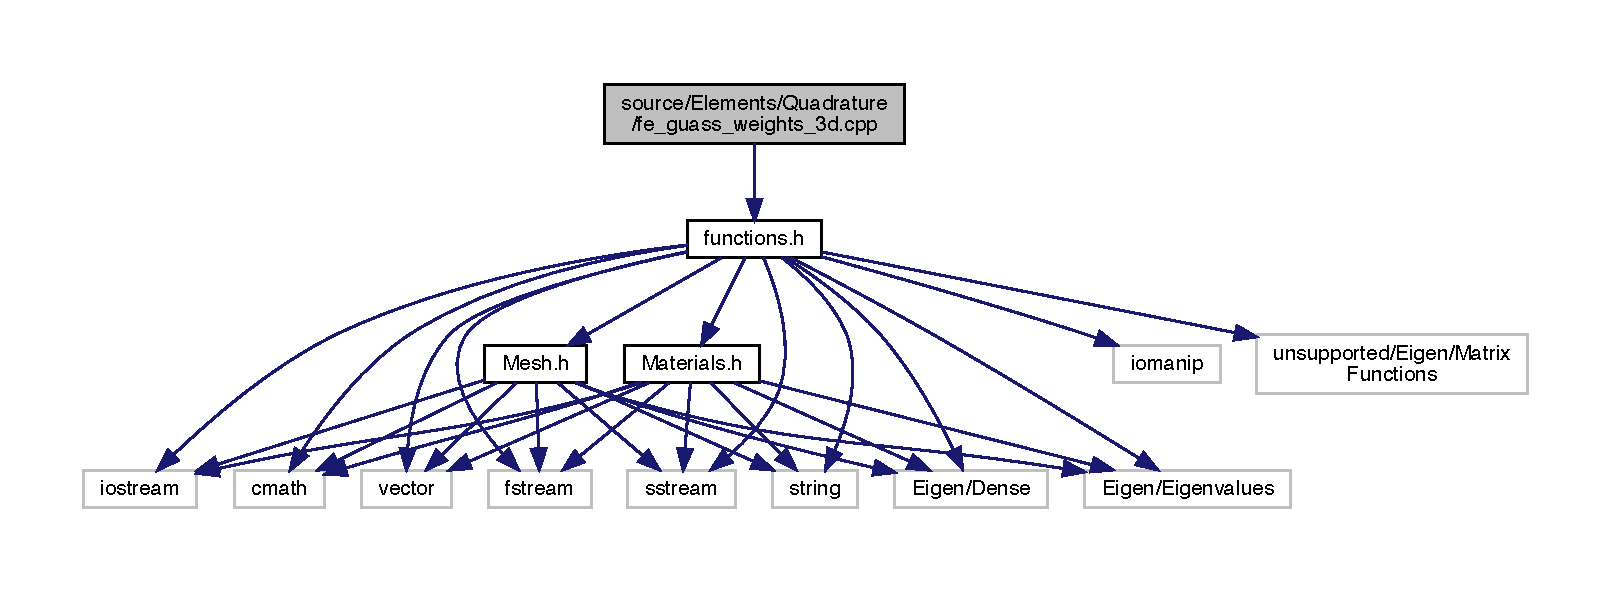
\includegraphics[width=350pt]{fe__guass__weights__3d_8cpp__incl}
\end{center}
\end{figure}
\subsection*{Functions}
\begin{DoxyCompactItemize}
\item 
Matrix\+Xd \hyperlink{fe__guass__weights__3d_8cpp_ad99b08ce65ae353e91486d7685c22024}{guass\+\_\+weights\+\_\+3d} (int \hyperlink{main_8cpp_aa789fe4d8a13fd0990b630909430d5d0}{ndof}, int nx, int ny, int nz)
\end{DoxyCompactItemize}


\subsection{Function Documentation}
\mbox{\Hypertarget{fe__guass__weights__3d_8cpp_ad99b08ce65ae353e91486d7685c22024}\label{fe__guass__weights__3d_8cpp_ad99b08ce65ae353e91486d7685c22024}} 
\index{fe\+\_\+guass\+\_\+weights\+\_\+3d.\+cpp@{fe\+\_\+guass\+\_\+weights\+\_\+3d.\+cpp}!guass\+\_\+weights\+\_\+3d@{guass\+\_\+weights\+\_\+3d}}
\index{guass\+\_\+weights\+\_\+3d@{guass\+\_\+weights\+\_\+3d}!fe\+\_\+guass\+\_\+weights\+\_\+3d.\+cpp@{fe\+\_\+guass\+\_\+weights\+\_\+3d.\+cpp}}
\subsubsection{\texorpdfstring{guass\+\_\+weights\+\_\+3d()}{guass\_weights\_3d()}}
{\footnotesize\ttfamily Matrix\+Xd guass\+\_\+weights\+\_\+3d (\begin{DoxyParamCaption}\item[{int}]{ndof,  }\item[{int}]{nx,  }\item[{int}]{ny,  }\item[{int}]{nz }\end{DoxyParamCaption})}

Creates a guass weight matrix in 3D 

Definition at line 5 of file fe\+\_\+guass\+\_\+weights\+\_\+3d.\+cpp.

Here is the call graph for this function\+:
\nopagebreak
\begin{figure}[H]
\begin{center}
\leavevmode
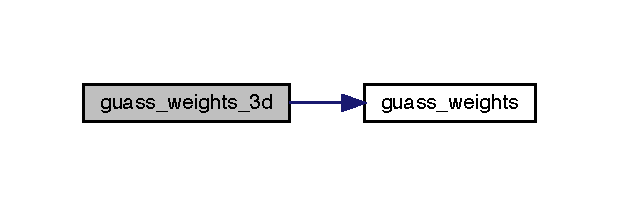
\includegraphics[width=297pt]{fe__guass__weights__3d_8cpp_ad99b08ce65ae353e91486d7685c22024_cgraph}
\end{center}
\end{figure}
Here is the caller graph for this function\+:
\nopagebreak
\begin{figure}[H]
\begin{center}
\leavevmode
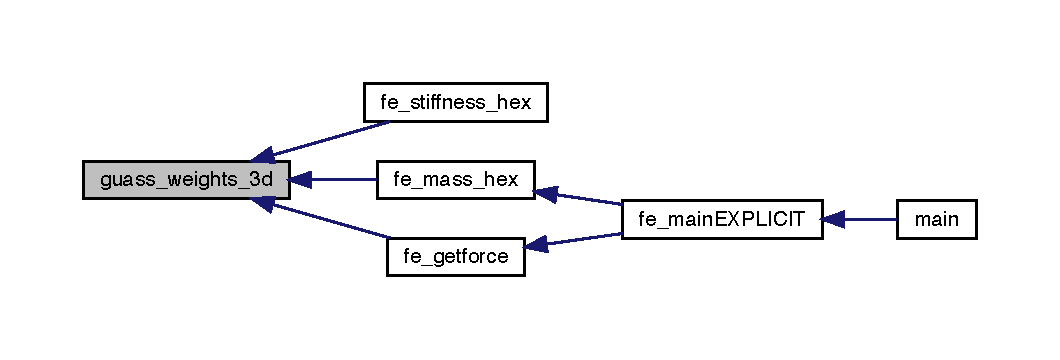
\includegraphics[width=350pt]{fe__guass__weights__3d_8cpp_ad99b08ce65ae353e91486d7685c22024_icgraph}
\end{center}
\end{figure}

\hypertarget{fe__dn__actual__8_8cpp}{}\section{source/\+Elements/\+Shape\+Functions/fe\+\_\+dn\+\_\+actual\+\_\+8.cpp File Reference}
\label{fe__dn__actual__8_8cpp}\index{source/\+Elements/\+Shape\+Functions/fe\+\_\+dn\+\_\+actual\+\_\+8.\+cpp@{source/\+Elements/\+Shape\+Functions/fe\+\_\+dn\+\_\+actual\+\_\+8.\+cpp}}
{\ttfamily \#include \char`\"{}functions.\+h\char`\"{}}\newline
Include dependency graph for fe\+\_\+dn\+\_\+actual\+\_\+8.\+cpp\+:
\nopagebreak
\begin{figure}[H]
\begin{center}
\leavevmode
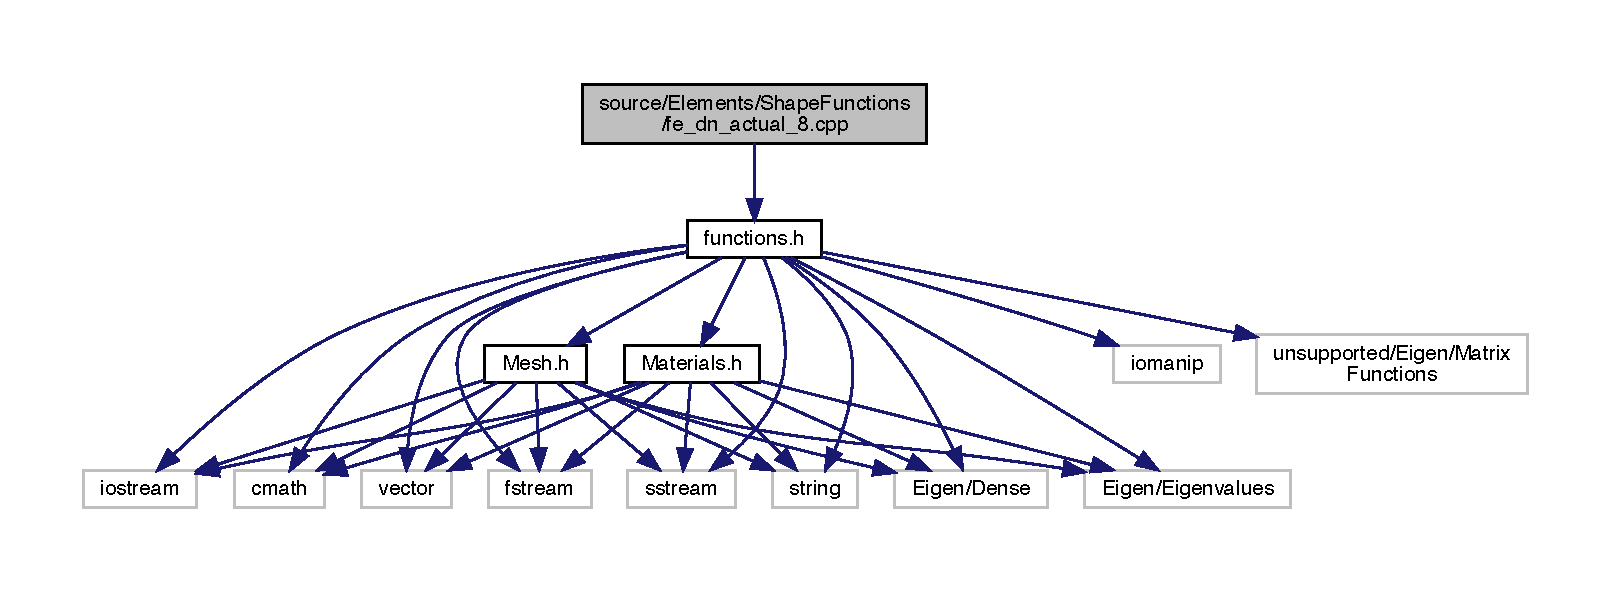
\includegraphics[width=350pt]{fe__dn__actual__8_8cpp__incl}
\end{center}
\end{figure}
\subsection*{Functions}
\begin{DoxyCompactItemize}
\item 
Vector\+Xd \hyperlink{fe__dn__actual__8_8cpp_afc6be1a5667e68156cb099e8da71170f}{fe\+\_\+dndx\+\_\+8} (int nnel, Vector\+Xd dndr, Vector\+Xd dnds, Vector\+Xd dndt, Matrix\+Xd inv\+Jacobian)
\item 
Vector\+Xd \hyperlink{fe__dn__actual__8_8cpp_a0572d7818e085c67f7fbb84eef8ecfb4}{fe\+\_\+dndy\+\_\+8} (int nnel, Vector\+Xd dndr, Vector\+Xd dnds, Vector\+Xd dndt, Matrix\+Xd inv\+Jacobian)
\item 
Vector\+Xd \hyperlink{fe__dn__actual__8_8cpp_aaf75db8433433807839c6ea17f2cf72c}{fe\+\_\+dndz\+\_\+8} (int nnel, Vector\+Xd dndr, Vector\+Xd dnds, Vector\+Xd dndt, Matrix\+Xd inv\+Jacobian)
\end{DoxyCompactItemize}


\subsection{Function Documentation}
\mbox{\Hypertarget{fe__dn__actual__8_8cpp_afc6be1a5667e68156cb099e8da71170f}\label{fe__dn__actual__8_8cpp_afc6be1a5667e68156cb099e8da71170f}} 
\index{fe\+\_\+dn\+\_\+actual\+\_\+8.\+cpp@{fe\+\_\+dn\+\_\+actual\+\_\+8.\+cpp}!fe\+\_\+dndx\+\_\+8@{fe\+\_\+dndx\+\_\+8}}
\index{fe\+\_\+dndx\+\_\+8@{fe\+\_\+dndx\+\_\+8}!fe\+\_\+dn\+\_\+actual\+\_\+8.\+cpp@{fe\+\_\+dn\+\_\+actual\+\_\+8.\+cpp}}
\subsubsection{\texorpdfstring{fe\+\_\+dndx\+\_\+8()}{fe\_dndx\_8()}}
{\footnotesize\ttfamily Vector\+Xd fe\+\_\+dndx\+\_\+8 (\begin{DoxyParamCaption}\item[{int}]{nnel,  }\item[{Vector\+Xd}]{dndr,  }\item[{Vector\+Xd}]{dnds,  }\item[{Vector\+Xd}]{dndt,  }\item[{Matrix\+Xd}]{inv\+Jacobian }\end{DoxyParamCaption})}

dndx of actual element calculates using jacobian and shape function derivates calculated in the isoparametric element 

Definition at line 6 of file fe\+\_\+dn\+\_\+actual\+\_\+8.\+cpp.

Here is the caller graph for this function\+:
\nopagebreak
\begin{figure}[H]
\begin{center}
\leavevmode
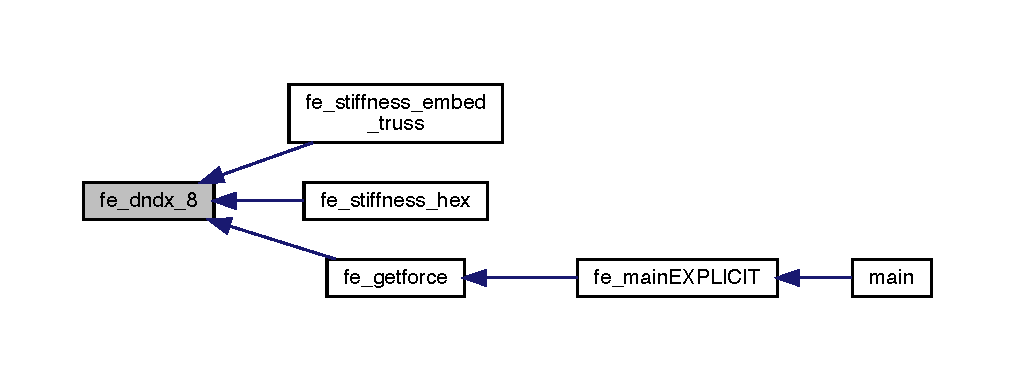
\includegraphics[width=350pt]{fe__dn__actual__8_8cpp_afc6be1a5667e68156cb099e8da71170f_icgraph}
\end{center}
\end{figure}
\mbox{\Hypertarget{fe__dn__actual__8_8cpp_a0572d7818e085c67f7fbb84eef8ecfb4}\label{fe__dn__actual__8_8cpp_a0572d7818e085c67f7fbb84eef8ecfb4}} 
\index{fe\+\_\+dn\+\_\+actual\+\_\+8.\+cpp@{fe\+\_\+dn\+\_\+actual\+\_\+8.\+cpp}!fe\+\_\+dndy\+\_\+8@{fe\+\_\+dndy\+\_\+8}}
\index{fe\+\_\+dndy\+\_\+8@{fe\+\_\+dndy\+\_\+8}!fe\+\_\+dn\+\_\+actual\+\_\+8.\+cpp@{fe\+\_\+dn\+\_\+actual\+\_\+8.\+cpp}}
\subsubsection{\texorpdfstring{fe\+\_\+dndy\+\_\+8()}{fe\_dndy\_8()}}
{\footnotesize\ttfamily Vector\+Xd fe\+\_\+dndy\+\_\+8 (\begin{DoxyParamCaption}\item[{int}]{nnel,  }\item[{Vector\+Xd}]{dndr,  }\item[{Vector\+Xd}]{dnds,  }\item[{Vector\+Xd}]{dndt,  }\item[{Matrix\+Xd}]{inv\+Jacobian }\end{DoxyParamCaption})}

dndy of actual element calculates using jacobian and shape function derivates calculated in the isoparametric element 

Definition at line 17 of file fe\+\_\+dn\+\_\+actual\+\_\+8.\+cpp.

Here is the caller graph for this function\+:
\nopagebreak
\begin{figure}[H]
\begin{center}
\leavevmode
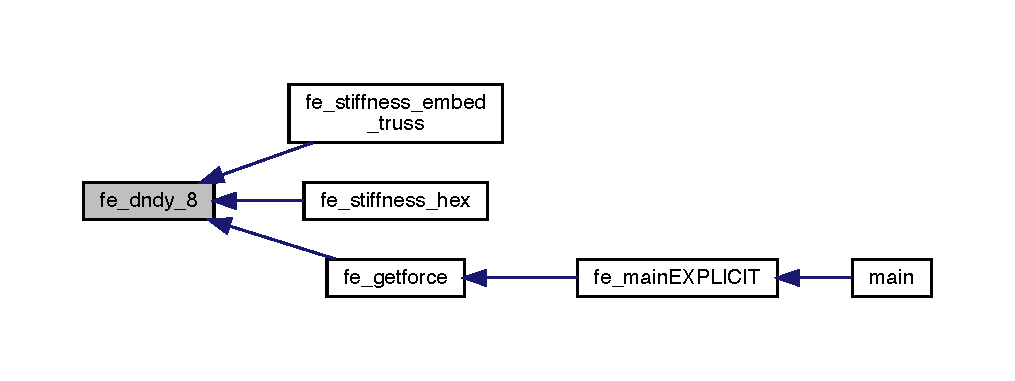
\includegraphics[width=350pt]{fe__dn__actual__8_8cpp_a0572d7818e085c67f7fbb84eef8ecfb4_icgraph}
\end{center}
\end{figure}
\mbox{\Hypertarget{fe__dn__actual__8_8cpp_aaf75db8433433807839c6ea17f2cf72c}\label{fe__dn__actual__8_8cpp_aaf75db8433433807839c6ea17f2cf72c}} 
\index{fe\+\_\+dn\+\_\+actual\+\_\+8.\+cpp@{fe\+\_\+dn\+\_\+actual\+\_\+8.\+cpp}!fe\+\_\+dndz\+\_\+8@{fe\+\_\+dndz\+\_\+8}}
\index{fe\+\_\+dndz\+\_\+8@{fe\+\_\+dndz\+\_\+8}!fe\+\_\+dn\+\_\+actual\+\_\+8.\+cpp@{fe\+\_\+dn\+\_\+actual\+\_\+8.\+cpp}}
\subsubsection{\texorpdfstring{fe\+\_\+dndz\+\_\+8()}{fe\_dndz\_8()}}
{\footnotesize\ttfamily Vector\+Xd fe\+\_\+dndz\+\_\+8 (\begin{DoxyParamCaption}\item[{int}]{nnel,  }\item[{Vector\+Xd}]{dndr,  }\item[{Vector\+Xd}]{dnds,  }\item[{Vector\+Xd}]{dndt,  }\item[{Matrix\+Xd}]{inv\+Jacobian }\end{DoxyParamCaption})}

dndz of actual element calculates using jacobian and shape function derivates calculated in the isoparametric element 

Definition at line 28 of file fe\+\_\+dn\+\_\+actual\+\_\+8.\+cpp.

Here is the caller graph for this function\+:
\nopagebreak
\begin{figure}[H]
\begin{center}
\leavevmode
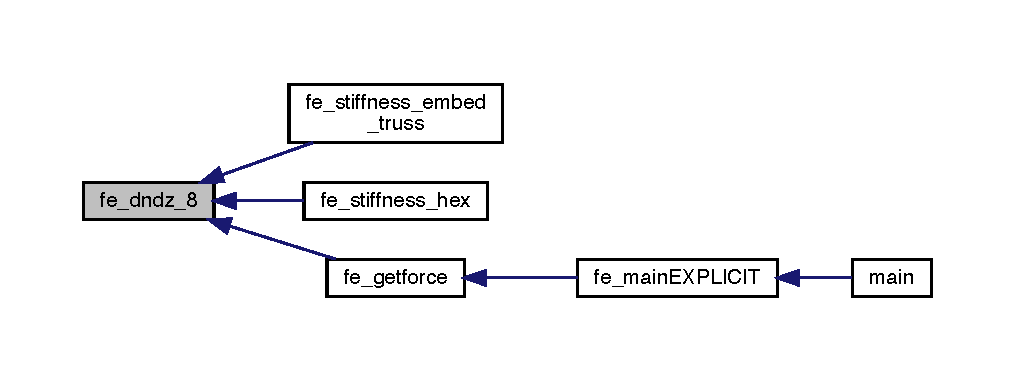
\includegraphics[width=350pt]{fe__dn__actual__8_8cpp_aaf75db8433433807839c6ea17f2cf72c_icgraph}
\end{center}
\end{figure}

\hypertarget{fe__dn__iso__8_8cpp}{}\section{/\+Users/vsg111/\+Dropbox/\+Work/\+Papers/\+Paper\+\_\+\+E\+E\+M\+\_\+\+Computational/\+E\+E\+M\+\_\+\+Dynamic/source/\+Elements/\+Shape\+Functions/fe\+\_\+dn\+\_\+iso\+\_\+8.cpp File Reference}
\label{fe__dn__iso__8_8cpp}\index{/\+Users/vsg111/\+Dropbox/\+Work/\+Papers/\+Paper\+\_\+\+E\+E\+M\+\_\+\+Computational/\+E\+E\+M\+\_\+\+Dynamic/source/\+Elements/\+Shape\+Functions/fe\+\_\+dn\+\_\+iso\+\_\+8.\+cpp@{/\+Users/vsg111/\+Dropbox/\+Work/\+Papers/\+Paper\+\_\+\+E\+E\+M\+\_\+\+Computational/\+E\+E\+M\+\_\+\+Dynamic/source/\+Elements/\+Shape\+Functions/fe\+\_\+dn\+\_\+iso\+\_\+8.\+cpp}}
{\ttfamily \#include \char`\"{}functions.\+h\char`\"{}}\newline
\subsection*{Functions}
\begin{DoxyCompactItemize}
\item 
Vector\+Xd \hyperlink{fe__dn__iso__8_8cpp_afc547bef246c057db6cbd04bf7f866a9}{fe\+\_\+dndr\+\_\+8} (double rvalue, double svalue, double tvalue)
\item 
Vector\+Xd \hyperlink{fe__dn__iso__8_8cpp_ac0b5524525e1f2e89bb064c15ab8e664}{fe\+\_\+dnds\+\_\+8} (double rvalue, double svalue, double tvalue)
\item 
Vector\+Xd \hyperlink{fe__dn__iso__8_8cpp_a57e8e5c9f740c98e4767f29c121c2d0a}{fe\+\_\+dndt\+\_\+8} (double rvalue, double svalue, double tvalue)
\end{DoxyCompactItemize}


\subsection{Function Documentation}
\mbox{\Hypertarget{fe__dn__iso__8_8cpp_afc547bef246c057db6cbd04bf7f866a9}\label{fe__dn__iso__8_8cpp_afc547bef246c057db6cbd04bf7f866a9}} 
\index{fe\+\_\+dn\+\_\+iso\+\_\+8.\+cpp@{fe\+\_\+dn\+\_\+iso\+\_\+8.\+cpp}!fe\+\_\+dndr\+\_\+8@{fe\+\_\+dndr\+\_\+8}}
\index{fe\+\_\+dndr\+\_\+8@{fe\+\_\+dndr\+\_\+8}!fe\+\_\+dn\+\_\+iso\+\_\+8.\+cpp@{fe\+\_\+dn\+\_\+iso\+\_\+8.\+cpp}}
\subsubsection{\texorpdfstring{fe\+\_\+dndr\+\_\+8()}{fe\_dndr\_8()}}
{\footnotesize\ttfamily Vector\+Xd fe\+\_\+dndr\+\_\+8 (\begin{DoxyParamCaption}\item[{double}]{rvalue,  }\item[{double}]{svalue,  }\item[{double}]{tvalue }\end{DoxyParamCaption})}

dndr of isoparametric element calculated for particular r, s, and t 

Definition at line 6 of file fe\+\_\+dn\+\_\+iso\+\_\+8.\+cpp.

\mbox{\Hypertarget{fe__dn__iso__8_8cpp_ac0b5524525e1f2e89bb064c15ab8e664}\label{fe__dn__iso__8_8cpp_ac0b5524525e1f2e89bb064c15ab8e664}} 
\index{fe\+\_\+dn\+\_\+iso\+\_\+8.\+cpp@{fe\+\_\+dn\+\_\+iso\+\_\+8.\+cpp}!fe\+\_\+dnds\+\_\+8@{fe\+\_\+dnds\+\_\+8}}
\index{fe\+\_\+dnds\+\_\+8@{fe\+\_\+dnds\+\_\+8}!fe\+\_\+dn\+\_\+iso\+\_\+8.\+cpp@{fe\+\_\+dn\+\_\+iso\+\_\+8.\+cpp}}
\subsubsection{\texorpdfstring{fe\+\_\+dnds\+\_\+8()}{fe\_dnds\_8()}}
{\footnotesize\ttfamily Vector\+Xd fe\+\_\+dnds\+\_\+8 (\begin{DoxyParamCaption}\item[{double}]{rvalue,  }\item[{double}]{svalue,  }\item[{double}]{tvalue }\end{DoxyParamCaption})}

dnds of isoparametric element calculated for particular r, s, and t 

Definition at line 44 of file fe\+\_\+dn\+\_\+iso\+\_\+8.\+cpp.

\mbox{\Hypertarget{fe__dn__iso__8_8cpp_a57e8e5c9f740c98e4767f29c121c2d0a}\label{fe__dn__iso__8_8cpp_a57e8e5c9f740c98e4767f29c121c2d0a}} 
\index{fe\+\_\+dn\+\_\+iso\+\_\+8.\+cpp@{fe\+\_\+dn\+\_\+iso\+\_\+8.\+cpp}!fe\+\_\+dndt\+\_\+8@{fe\+\_\+dndt\+\_\+8}}
\index{fe\+\_\+dndt\+\_\+8@{fe\+\_\+dndt\+\_\+8}!fe\+\_\+dn\+\_\+iso\+\_\+8.\+cpp@{fe\+\_\+dn\+\_\+iso\+\_\+8.\+cpp}}
\subsubsection{\texorpdfstring{fe\+\_\+dndt\+\_\+8()}{fe\_dndt\_8()}}
{\footnotesize\ttfamily Vector\+Xd fe\+\_\+dndt\+\_\+8 (\begin{DoxyParamCaption}\item[{double}]{rvalue,  }\item[{double}]{svalue,  }\item[{double}]{tvalue }\end{DoxyParamCaption})}

dndt of isoparametric element calculated for particular r, s, and t 

Definition at line 82 of file fe\+\_\+dn\+\_\+iso\+\_\+8.\+cpp.


\hypertarget{fe__shape_matrix_8cpp}{}\section{/\+Users/vsg111/\+Dropbox/\+Work/\+Papers/\+Paper\+\_\+\+E\+E\+M\+\_\+\+Computational/\+E\+E\+M\+\_\+\+Dynamic/source/\+Elements/\+Shape\+Functions/fe\+\_\+shape\+Matrix.cpp File Reference}
\label{fe__shape_matrix_8cpp}\index{/\+Users/vsg111/\+Dropbox/\+Work/\+Papers/\+Paper\+\_\+\+E\+E\+M\+\_\+\+Computational/\+E\+E\+M\+\_\+\+Dynamic/source/\+Elements/\+Shape\+Functions/fe\+\_\+shape\+Matrix.\+cpp@{/\+Users/vsg111/\+Dropbox/\+Work/\+Papers/\+Paper\+\_\+\+E\+E\+M\+\_\+\+Computational/\+E\+E\+M\+\_\+\+Dynamic/source/\+Elements/\+Shape\+Functions/fe\+\_\+shape\+Matrix.\+cpp}}
{\ttfamily \#include \char`\"{}functions.\+h\char`\"{}}\newline
\subsection*{Functions}
\begin{DoxyCompactItemize}
\item 
Matrix\+Xd \hyperlink{fe__shape_matrix_8cpp_a98fae74dde5fe33a7062e7457a2d3227}{fe\+\_\+shape\+Matrix} (int edof, int nnel, Vector\+Xd shapes)
\end{DoxyCompactItemize}


\subsection{Function Documentation}
\mbox{\Hypertarget{fe__shape_matrix_8cpp_a98fae74dde5fe33a7062e7457a2d3227}\label{fe__shape_matrix_8cpp_a98fae74dde5fe33a7062e7457a2d3227}} 
\index{fe\+\_\+shape\+Matrix.\+cpp@{fe\+\_\+shape\+Matrix.\+cpp}!fe\+\_\+shape\+Matrix@{fe\+\_\+shape\+Matrix}}
\index{fe\+\_\+shape\+Matrix@{fe\+\_\+shape\+Matrix}!fe\+\_\+shape\+Matrix.\+cpp@{fe\+\_\+shape\+Matrix.\+cpp}}
\subsubsection{\texorpdfstring{fe\+\_\+shape\+Matrix()}{fe\_shapeMatrix()}}
{\footnotesize\ttfamily Matrix\+Xd fe\+\_\+shape\+Matrix (\begin{DoxyParamCaption}\item[{int}]{edof,  }\item[{int}]{nnel,  }\item[{Vector\+Xd}]{shapes }\end{DoxyParamCaption})}

Outputs the shape function matrix for an element 

Definition at line 7 of file fe\+\_\+shape\+Matrix.\+cpp.


\hypertarget{fe__shapes_8cpp}{}\section{source/\+Elements/\+Shape\+Functions/fe\+\_\+shapes.cpp File Reference}
\label{fe__shapes_8cpp}\index{source/\+Elements/\+Shape\+Functions/fe\+\_\+shapes.\+cpp@{source/\+Elements/\+Shape\+Functions/fe\+\_\+shapes.\+cpp}}
{\ttfamily \#include \char`\"{}functions.\+h\char`\"{}}\newline
Include dependency graph for fe\+\_\+shapes.\+cpp\+:
\nopagebreak
\begin{figure}[H]
\begin{center}
\leavevmode
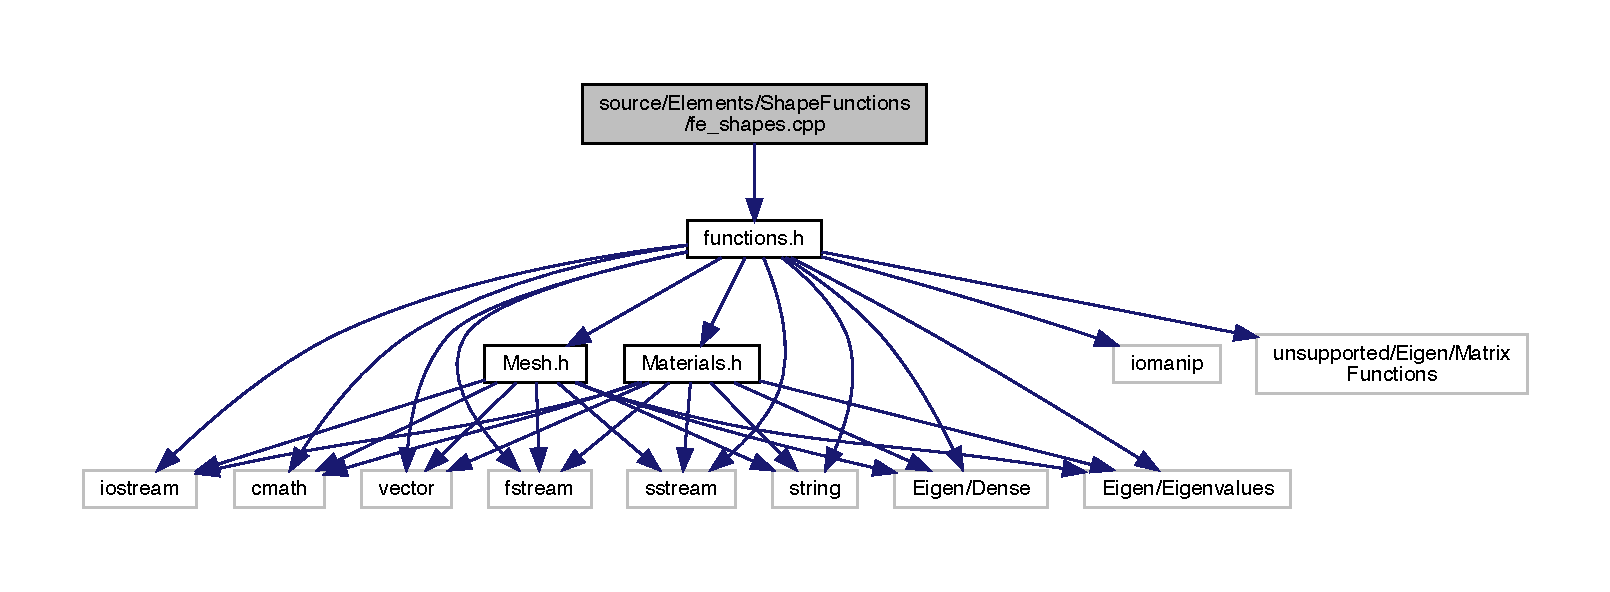
\includegraphics[width=350pt]{fe__shapes_8cpp__incl}
\end{center}
\end{figure}
\subsection*{Functions}
\begin{DoxyCompactItemize}
\item 
Vector\+Xd \hyperlink{fe__shapes_8cpp_ab77a3a6d6f6b436d7e8c600bb0869927}{fe\+\_\+shapes\+\_\+8} (double rvalue, double svalue, double tvalue)
\end{DoxyCompactItemize}


\subsection{Function Documentation}
\mbox{\Hypertarget{fe__shapes_8cpp_ab77a3a6d6f6b436d7e8c600bb0869927}\label{fe__shapes_8cpp_ab77a3a6d6f6b436d7e8c600bb0869927}} 
\index{fe\+\_\+shapes.\+cpp@{fe\+\_\+shapes.\+cpp}!fe\+\_\+shapes\+\_\+8@{fe\+\_\+shapes\+\_\+8}}
\index{fe\+\_\+shapes\+\_\+8@{fe\+\_\+shapes\+\_\+8}!fe\+\_\+shapes.\+cpp@{fe\+\_\+shapes.\+cpp}}
\subsubsection{\texorpdfstring{fe\+\_\+shapes\+\_\+8()}{fe\_shapes\_8()}}
{\footnotesize\ttfamily Vector\+Xd fe\+\_\+shapes\+\_\+8 (\begin{DoxyParamCaption}\item[{double}]{rvalue,  }\item[{double}]{svalue,  }\item[{double}]{tvalue }\end{DoxyParamCaption})}

Creates the shape functions for an 8 noded element 

Definition at line 7 of file fe\+\_\+shapes.\+cpp.

Here is the caller graph for this function\+:
\nopagebreak
\begin{figure}[H]
\begin{center}
\leavevmode
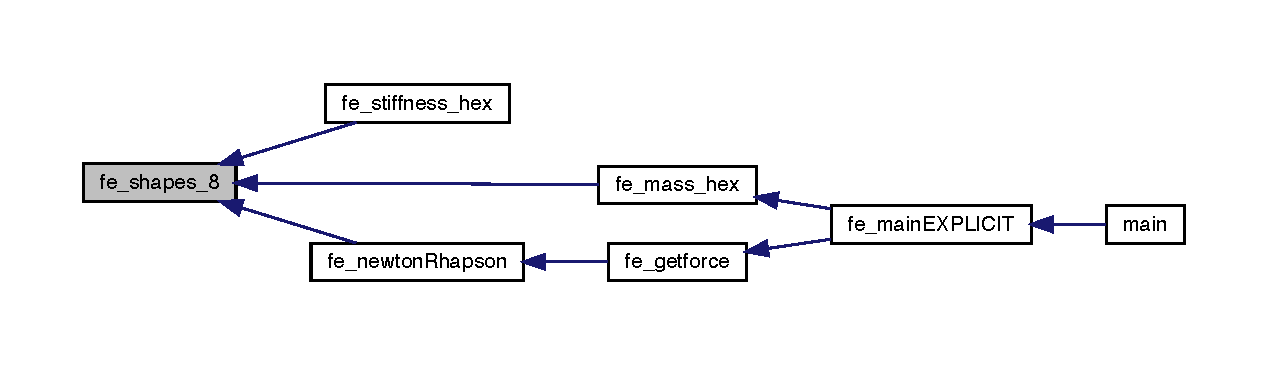
\includegraphics[width=350pt]{fe__shapes_8cpp_ab77a3a6d6f6b436d7e8c600bb0869927_icgraph}
\end{center}
\end{figure}

\hypertarget{fe__assemble__mass_8cpp}{}\section{/\+Users/vsg111/\+Dropbox/\+Work/\+Papers/\+Paper\+\_\+\+E\+E\+M\+\_\+\+Computational/\+E\+E\+M\+\_\+\+Dynamic/source/\+Elements/\+Global-\/\+Local/fe\+\_\+assemble\+\_\+mass.cpp File Reference}
\label{fe__assemble__mass_8cpp}\index{/\+Users/vsg111/\+Dropbox/\+Work/\+Papers/\+Paper\+\_\+\+E\+E\+M\+\_\+\+Computational/\+E\+E\+M\+\_\+\+Dynamic/source/\+Elements/\+Global-\/\+Local/fe\+\_\+assemble\+\_\+mass.\+cpp@{/\+Users/vsg111/\+Dropbox/\+Work/\+Papers/\+Paper\+\_\+\+E\+E\+M\+\_\+\+Computational/\+E\+E\+M\+\_\+\+Dynamic/source/\+Elements/\+Global-\/\+Local/fe\+\_\+assemble\+\_\+mass.\+cpp}}
{\ttfamily \#include $<$iostream$>$}\newline
{\ttfamily \#include \char`\"{}functions.\+h\char`\"{}}\newline
\subsection*{Functions}
\begin{DoxyCompactItemize}
\item 
Matrix\+Xd \hyperlink{fe__assemble__mass_8cpp_a04f569c566ca4fbea3b3a2a13cdd0af5}{fe\+\_\+assemble\+\_\+mass} (Matrix\+Xd mm, Matrix\+Xd m, Vector\+Xi node\+\_\+list, int sdof)
\end{DoxyCompactItemize}


\subsection{Function Documentation}
\mbox{\Hypertarget{fe__assemble__mass_8cpp_a04f569c566ca4fbea3b3a2a13cdd0af5}\label{fe__assemble__mass_8cpp_a04f569c566ca4fbea3b3a2a13cdd0af5}} 
\index{fe\+\_\+assemble\+\_\+mass.\+cpp@{fe\+\_\+assemble\+\_\+mass.\+cpp}!fe\+\_\+assemble\+\_\+mass@{fe\+\_\+assemble\+\_\+mass}}
\index{fe\+\_\+assemble\+\_\+mass@{fe\+\_\+assemble\+\_\+mass}!fe\+\_\+assemble\+\_\+mass.\+cpp@{fe\+\_\+assemble\+\_\+mass.\+cpp}}
\subsubsection{\texorpdfstring{fe\+\_\+assemble\+\_\+mass()}{fe\_assemble\_mass()}}
{\footnotesize\ttfamily Matrix\+Xd fe\+\_\+assemble\+\_\+mass (\begin{DoxyParamCaption}\item[{Matrix\+Xd}]{mm,  }\item[{Matrix\+Xd}]{m,  }\item[{Vector\+Xi}]{node\+\_\+list,  }\item[{int}]{sdof }\end{DoxyParamCaption})}

Assembles the global mass matrix 

Definition at line 24 of file fe\+\_\+assemble\+\_\+mass.\+cpp.


\hypertarget{fe__find__index_8cpp}{}\section{source/\+F\+E\+M/\+Assembly-\/\+Global-\/\+Local/fe\+\_\+find\+\_\+index.cpp File Reference}
\label{fe__find__index_8cpp}\index{source/\+F\+E\+M/\+Assembly-\/\+Global-\/\+Local/fe\+\_\+find\+\_\+index.\+cpp@{source/\+F\+E\+M/\+Assembly-\/\+Global-\/\+Local/fe\+\_\+find\+\_\+index.\+cpp}}
{\ttfamily \#include $<$iostream$>$}\newline
{\ttfamily \#include \char`\"{}functions.\+h\char`\"{}}\newline
Include dependency graph for fe\+\_\+find\+\_\+index.\+cpp\+:
\nopagebreak
\begin{figure}[H]
\begin{center}
\leavevmode
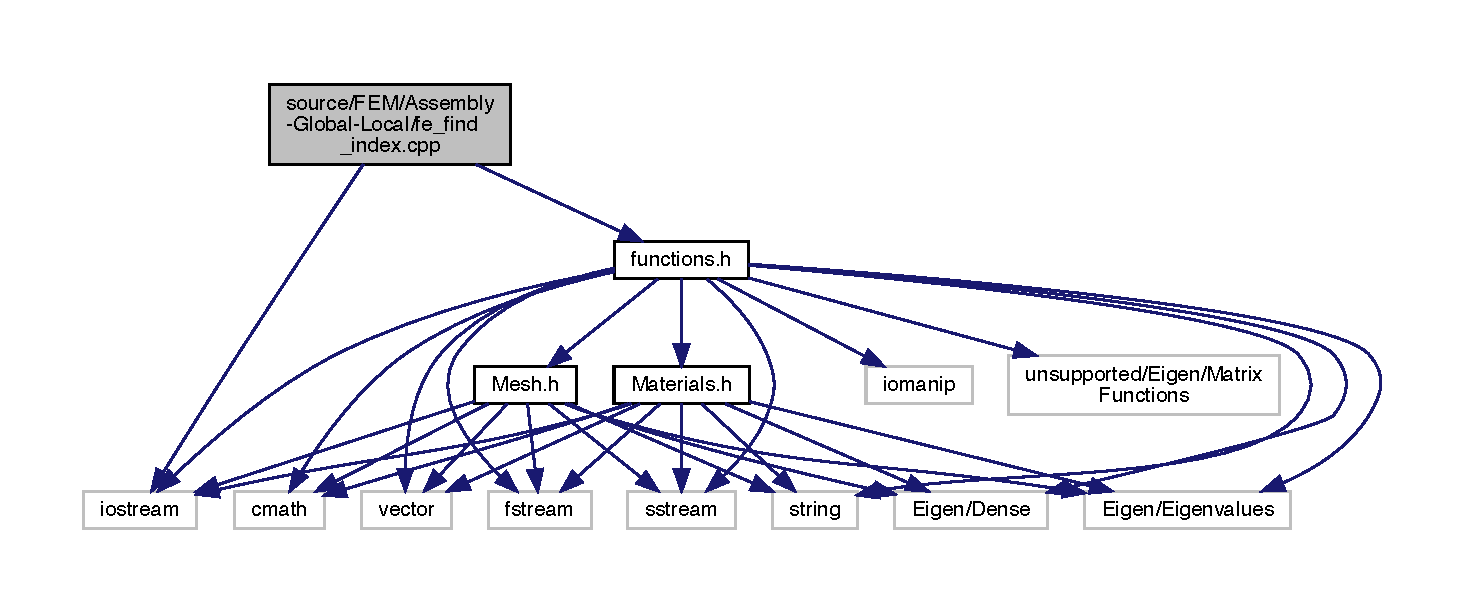
\includegraphics[width=350pt]{fe__find__index_8cpp__incl}
\end{center}
\end{figure}
\subsection*{Functions}
\begin{DoxyCompactItemize}
\item 
Vector\+Xi \hyperlink{fe__find__index_8cpp_ae4dbe24b761cafa3577afab76726b382}{fe\+\_\+find\+\_\+index} (Vector\+Xi node\+\_\+list)
\end{DoxyCompactItemize}


\subsection{Function Documentation}
\mbox{\Hypertarget{fe__find__index_8cpp_ae4dbe24b761cafa3577afab76726b382}\label{fe__find__index_8cpp_ae4dbe24b761cafa3577afab76726b382}} 
\index{fe\+\_\+find\+\_\+index.\+cpp@{fe\+\_\+find\+\_\+index.\+cpp}!fe\+\_\+find\+\_\+index@{fe\+\_\+find\+\_\+index}}
\index{fe\+\_\+find\+\_\+index@{fe\+\_\+find\+\_\+index}!fe\+\_\+find\+\_\+index.\+cpp@{fe\+\_\+find\+\_\+index.\+cpp}}
\subsubsection{\texorpdfstring{fe\+\_\+find\+\_\+index()}{fe\_find\_index()}}
{\footnotesize\ttfamily Vector\+Xi fe\+\_\+find\+\_\+index (\begin{DoxyParamCaption}\item[{Vector\+Xi}]{node\+\_\+list }\end{DoxyParamCaption})}

Find the index based on the D\+OF of a particular node 

Definition at line 16 of file fe\+\_\+find\+\_\+index.\+cpp.

Here is the caller graph for this function\+:
\nopagebreak
\begin{figure}[H]
\begin{center}
\leavevmode
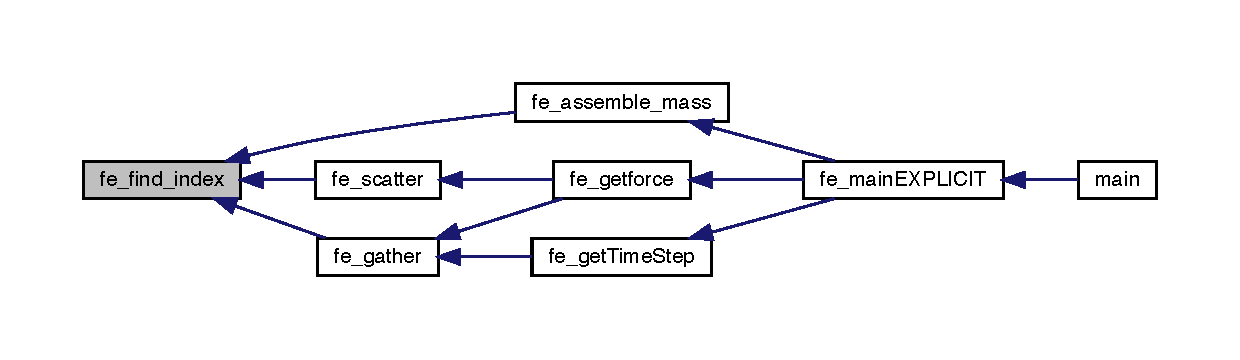
\includegraphics[width=350pt]{fe__find__index_8cpp_ae4dbe24b761cafa3577afab76726b382_icgraph}
\end{center}
\end{figure}

\hypertarget{fe__gather_8cpp}{}\section{source/\+F\+E\+M/\+Assembly-\/\+Global-\/\+Local/fe\+\_\+gather.cpp File Reference}
\label{fe__gather_8cpp}\index{source/\+F\+E\+M/\+Assembly-\/\+Global-\/\+Local/fe\+\_\+gather.\+cpp@{source/\+F\+E\+M/\+Assembly-\/\+Global-\/\+Local/fe\+\_\+gather.\+cpp}}
{\ttfamily \#include $<$iostream$>$}\newline
{\ttfamily \#include \char`\"{}functions.\+h\char`\"{}}\newline
Include dependency graph for fe\+\_\+gather.\+cpp\+:
\nopagebreak
\begin{figure}[H]
\begin{center}
\leavevmode
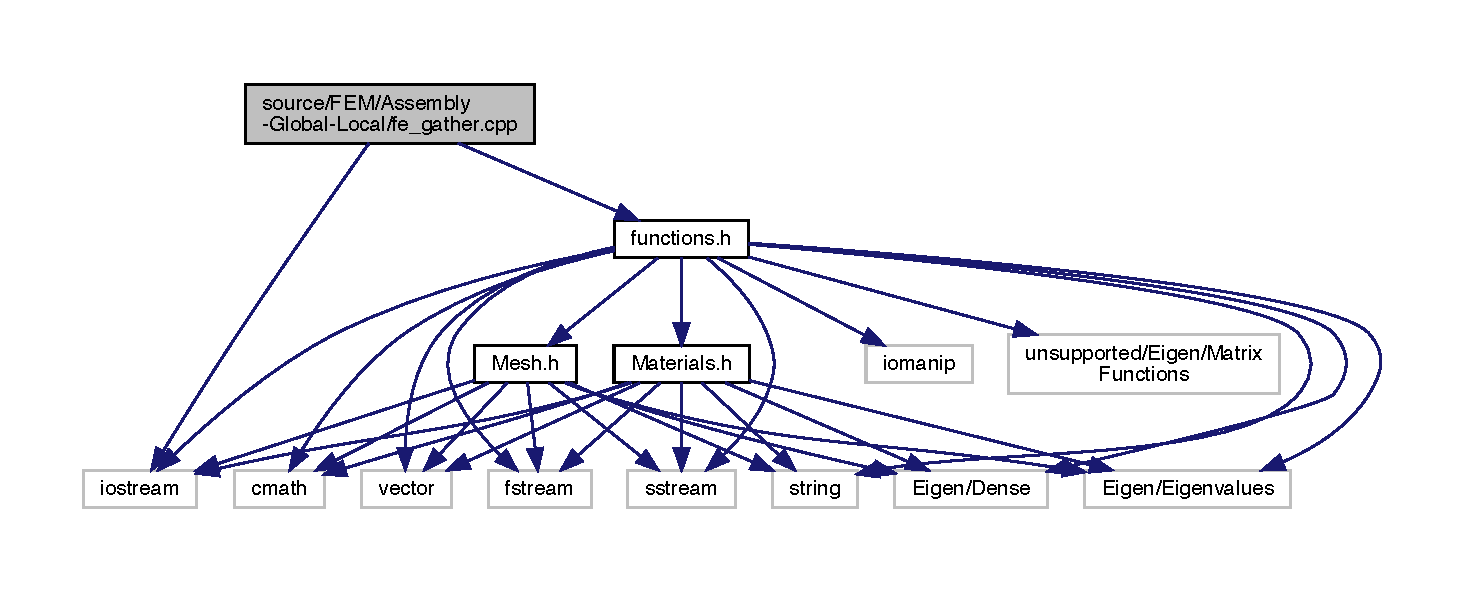
\includegraphics[width=350pt]{fe__gather_8cpp__incl}
\end{center}
\end{figure}
\subsection*{Functions}
\begin{DoxyCompactItemize}
\item 
Vector\+Xd \hyperlink{fe__gather_8cpp_ab5053cb12ac67971a7836346e2839725}{fe\+\_\+gather} (Vector\+Xd global\+\_\+vec, Vector\+Xd local\+\_\+vec, Vector\+Xi node\+\_\+list, int sdof)
\end{DoxyCompactItemize}


\subsection{Function Documentation}
\mbox{\Hypertarget{fe__gather_8cpp_ab5053cb12ac67971a7836346e2839725}\label{fe__gather_8cpp_ab5053cb12ac67971a7836346e2839725}} 
\index{fe\+\_\+gather.\+cpp@{fe\+\_\+gather.\+cpp}!fe\+\_\+gather@{fe\+\_\+gather}}
\index{fe\+\_\+gather@{fe\+\_\+gather}!fe\+\_\+gather.\+cpp@{fe\+\_\+gather.\+cpp}}
\subsubsection{\texorpdfstring{fe\+\_\+gather()}{fe\_gather()}}
{\footnotesize\ttfamily Vector\+Xd fe\+\_\+gather (\begin{DoxyParamCaption}\item[{Vector\+Xd}]{global\+\_\+vec,  }\item[{Vector\+Xd}]{local\+\_\+vec,  }\item[{Vector\+Xi}]{node\+\_\+list,  }\item[{int}]{sdof }\end{DoxyParamCaption})}

Creates element level vector (displacement, velocity, acceleration etc.) from a system level vector 

Definition at line 6 of file fe\+\_\+gather.\+cpp.

Here is the call graph for this function\+:
\nopagebreak
\begin{figure}[H]
\begin{center}
\leavevmode
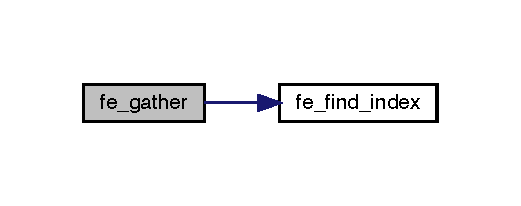
\includegraphics[width=250pt]{fe__gather_8cpp_ab5053cb12ac67971a7836346e2839725_cgraph}
\end{center}
\end{figure}
Here is the caller graph for this function\+:
\nopagebreak
\begin{figure}[H]
\begin{center}
\leavevmode
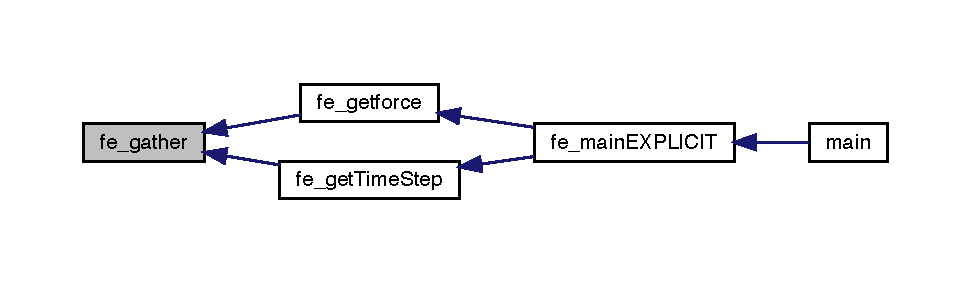
\includegraphics[width=350pt]{fe__gather_8cpp_ab5053cb12ac67971a7836346e2839725_icgraph}
\end{center}
\end{figure}

\hypertarget{fe__scatter_8cpp}{}\section{source/\+F\+E\+M/\+Assembly-\/\+Global-\/\+Local/fe\+\_\+scatter.cpp File Reference}
\label{fe__scatter_8cpp}\index{source/\+F\+E\+M/\+Assembly-\/\+Global-\/\+Local/fe\+\_\+scatter.\+cpp@{source/\+F\+E\+M/\+Assembly-\/\+Global-\/\+Local/fe\+\_\+scatter.\+cpp}}
{\ttfamily \#include $<$iostream$>$}\newline
{\ttfamily \#include \char`\"{}functions.\+h\char`\"{}}\newline
Include dependency graph for fe\+\_\+scatter.\+cpp\+:
\nopagebreak
\begin{figure}[H]
\begin{center}
\leavevmode
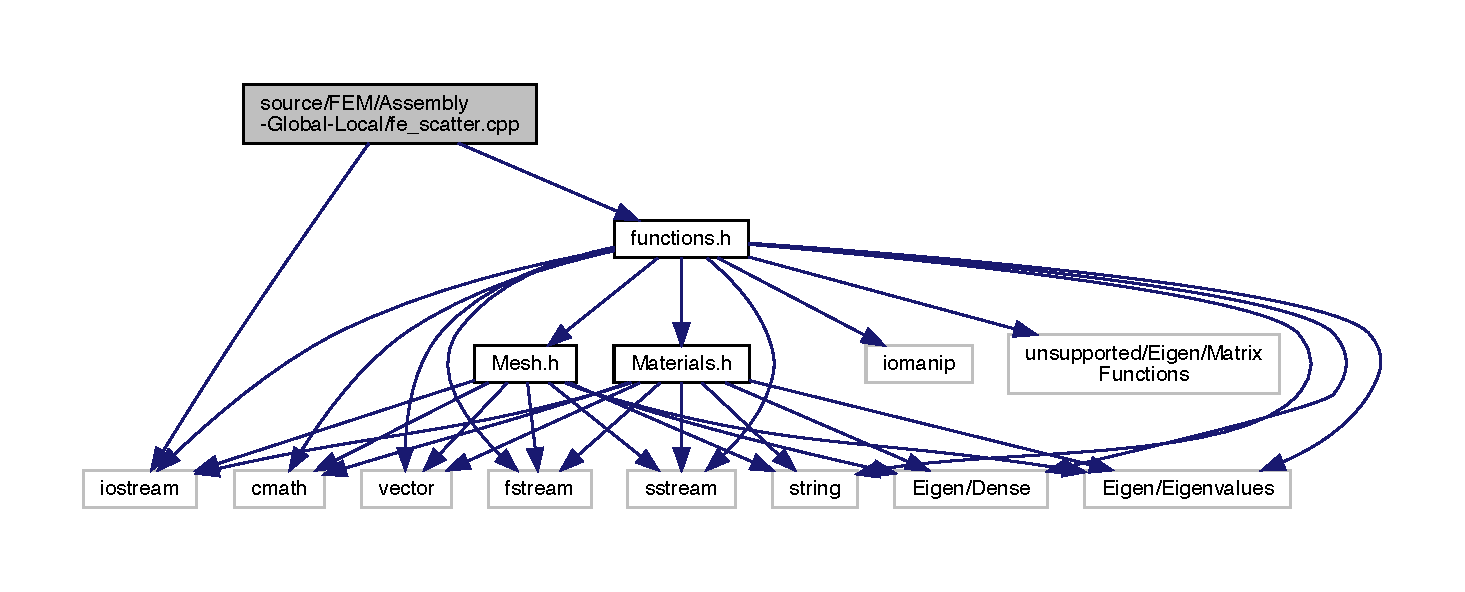
\includegraphics[width=350pt]{fe__scatter_8cpp__incl}
\end{center}
\end{figure}
\subsection*{Functions}
\begin{DoxyCompactItemize}
\item 
Vector\+Xd \hyperlink{fe__scatter_8cpp_a6b8344e12f9005795f93f60ddda26c5c}{fe\+\_\+scatter} (Vector\+Xd global\+\_\+vec, Vector\+Xd local\+\_\+vec, Vector\+Xi node\+\_\+list, int sdof)
\end{DoxyCompactItemize}


\subsection{Function Documentation}
\mbox{\Hypertarget{fe__scatter_8cpp_a6b8344e12f9005795f93f60ddda26c5c}\label{fe__scatter_8cpp_a6b8344e12f9005795f93f60ddda26c5c}} 
\index{fe\+\_\+scatter.\+cpp@{fe\+\_\+scatter.\+cpp}!fe\+\_\+scatter@{fe\+\_\+scatter}}
\index{fe\+\_\+scatter@{fe\+\_\+scatter}!fe\+\_\+scatter.\+cpp@{fe\+\_\+scatter.\+cpp}}
\subsubsection{\texorpdfstring{fe\+\_\+scatter()}{fe\_scatter()}}
{\footnotesize\ttfamily Vector\+Xd fe\+\_\+scatter (\begin{DoxyParamCaption}\item[{Vector\+Xd}]{global\+\_\+vec,  }\item[{Vector\+Xd}]{local\+\_\+vec,  }\item[{Vector\+Xi}]{node\+\_\+list,  }\item[{int}]{sdof }\end{DoxyParamCaption})}

Updates a system level vector based on the element level vector 

Definition at line 6 of file fe\+\_\+scatter.\+cpp.

Here is the call graph for this function\+:
\nopagebreak
\begin{figure}[H]
\begin{center}
\leavevmode
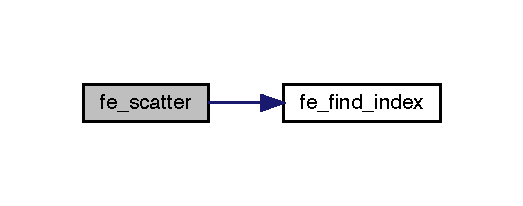
\includegraphics[width=251pt]{fe__scatter_8cpp_a6b8344e12f9005795f93f60ddda26c5c_cgraph}
\end{center}
\end{figure}
Here is the caller graph for this function\+:
\nopagebreak
\begin{figure}[H]
\begin{center}
\leavevmode
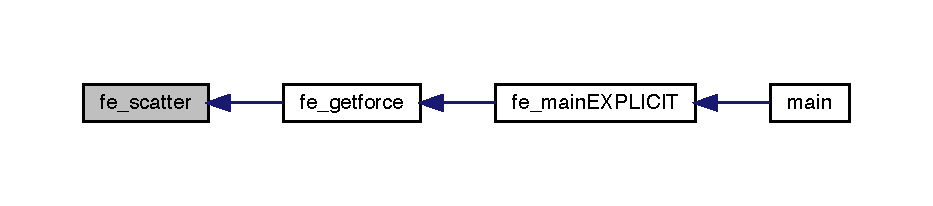
\includegraphics[width=350pt]{fe__scatter_8cpp_a6b8344e12f9005795f93f60ddda26c5c_icgraph}
\end{center}
\end{figure}

\hypertarget{fe__apply__bc_8cpp}{}\section{source/\+F\+E\+M/\+Boundary\+Conditions/fe\+\_\+apply\+\_\+bc.cpp File Reference}
\label{fe__apply__bc_8cpp}\index{source/\+F\+E\+M/\+Boundary\+Conditions/fe\+\_\+apply\+\_\+bc.\+cpp@{source/\+F\+E\+M/\+Boundary\+Conditions/fe\+\_\+apply\+\_\+bc.\+cpp}}
{\ttfamily \#include \char`\"{}functions.\+h\char`\"{}}\newline
Include dependency graph for fe\+\_\+apply\+\_\+bc.\+cpp\+:
\nopagebreak
\begin{figure}[H]
\begin{center}
\leavevmode
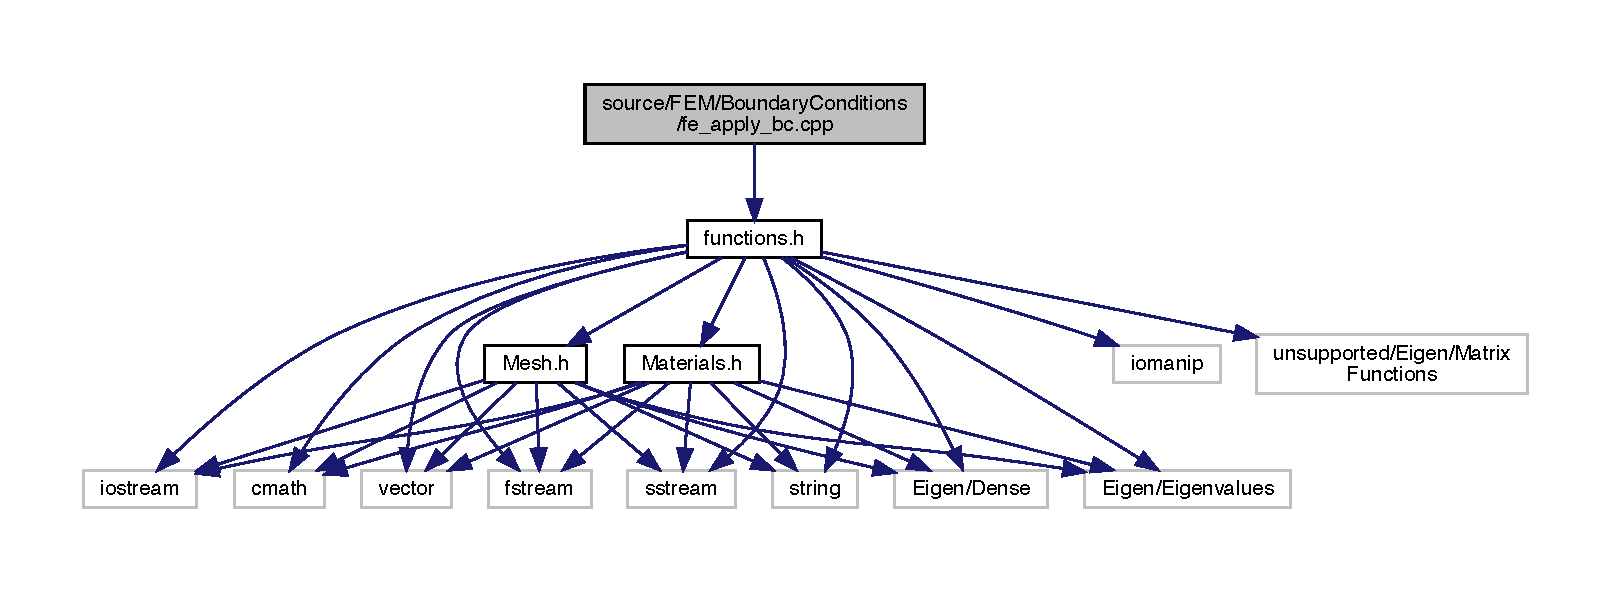
\includegraphics[width=350pt]{fe__apply__bc_8cpp__incl}
\end{center}
\end{figure}
\subsection*{Functions}
\begin{DoxyCompactItemize}
\item 
Vector\+Xd \hyperlink{fe__apply__bc_8cpp_af42938e5b32edb33ef4a35866949eba6}{fe\+\_\+apply\+\_\+bc\+\_\+displacement} (Vector\+Xd U, double time)
\item 
Vector\+Xd \hyperlink{fe__apply__bc_8cpp_aba32cc24bd74a4965c560fa62c5b213e}{fe\+\_\+apply\+\_\+bc\+\_\+load} (Vector\+Xd fe, double time)
\item 
Matrix\+Xd \hyperlink{fe__apply__bc_8cpp_a3c73fda948017ac96aeb19889cfc1cba}{fe\+\_\+apply\+\_\+bc\+\_\+stiffness} (Matrix\+Xd kk, Vector\+Xi \hyperlink{main_8cpp_a389e085bd7632077f619ea67d3fb4087}{bcdof}, Vector\+Xd \hyperlink{main_8cpp_a3a53182d9f97dc5acff0a10125857cfb}{bcval})
\end{DoxyCompactItemize}


\subsection{Function Documentation}
\mbox{\Hypertarget{fe__apply__bc_8cpp_af42938e5b32edb33ef4a35866949eba6}\label{fe__apply__bc_8cpp_af42938e5b32edb33ef4a35866949eba6}} 
\index{fe\+\_\+apply\+\_\+bc.\+cpp@{fe\+\_\+apply\+\_\+bc.\+cpp}!fe\+\_\+apply\+\_\+bc\+\_\+displacement@{fe\+\_\+apply\+\_\+bc\+\_\+displacement}}
\index{fe\+\_\+apply\+\_\+bc\+\_\+displacement@{fe\+\_\+apply\+\_\+bc\+\_\+displacement}!fe\+\_\+apply\+\_\+bc.\+cpp@{fe\+\_\+apply\+\_\+bc.\+cpp}}
\subsubsection{\texorpdfstring{fe\+\_\+apply\+\_\+bc\+\_\+displacement()}{fe\_apply\_bc\_displacement()}}
{\footnotesize\ttfamily Vector\+Xd fe\+\_\+apply\+\_\+bc\+\_\+displacement (\begin{DoxyParamCaption}\item[{Vector\+Xd}]{U,  }\item[{double}]{time }\end{DoxyParamCaption})}



Definition at line 5 of file fe\+\_\+apply\+\_\+bc.\+cpp.

Here is the call graph for this function\+:
\nopagebreak
\begin{figure}[H]
\begin{center}
\leavevmode
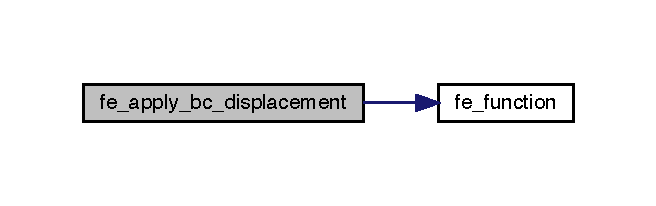
\includegraphics[width=315pt]{fe__apply__bc_8cpp_af42938e5b32edb33ef4a35866949eba6_cgraph}
\end{center}
\end{figure}
Here is the caller graph for this function\+:
\nopagebreak
\begin{figure}[H]
\begin{center}
\leavevmode
\includegraphics[width=350pt]{fe__apply__bc_8cpp_af42938e5b32edb33ef4a35866949eba6_icgraph}
\end{center}
\end{figure}
\mbox{\Hypertarget{fe__apply__bc_8cpp_aba32cc24bd74a4965c560fa62c5b213e}\label{fe__apply__bc_8cpp_aba32cc24bd74a4965c560fa62c5b213e}} 
\index{fe\+\_\+apply\+\_\+bc.\+cpp@{fe\+\_\+apply\+\_\+bc.\+cpp}!fe\+\_\+apply\+\_\+bc\+\_\+load@{fe\+\_\+apply\+\_\+bc\+\_\+load}}
\index{fe\+\_\+apply\+\_\+bc\+\_\+load@{fe\+\_\+apply\+\_\+bc\+\_\+load}!fe\+\_\+apply\+\_\+bc.\+cpp@{fe\+\_\+apply\+\_\+bc.\+cpp}}
\subsubsection{\texorpdfstring{fe\+\_\+apply\+\_\+bc\+\_\+load()}{fe\_apply\_bc\_load()}}
{\footnotesize\ttfamily Vector\+Xd fe\+\_\+apply\+\_\+bc\+\_\+load (\begin{DoxyParamCaption}\item[{Vector\+Xd}]{fe,  }\item[{double}]{time }\end{DoxyParamCaption})}



Definition at line 24 of file fe\+\_\+apply\+\_\+bc.\+cpp.

Here is the call graph for this function\+:
\nopagebreak
\begin{figure}[H]
\begin{center}
\leavevmode
\includegraphics[width=275pt]{fe__apply__bc_8cpp_aba32cc24bd74a4965c560fa62c5b213e_cgraph}
\end{center}
\end{figure}
Here is the caller graph for this function\+:
\nopagebreak
\begin{figure}[H]
\begin{center}
\leavevmode
\includegraphics[width=350pt]{fe__apply__bc_8cpp_aba32cc24bd74a4965c560fa62c5b213e_icgraph}
\end{center}
\end{figure}
\mbox{\Hypertarget{fe__apply__bc_8cpp_a3c73fda948017ac96aeb19889cfc1cba}\label{fe__apply__bc_8cpp_a3c73fda948017ac96aeb19889cfc1cba}} 
\index{fe\+\_\+apply\+\_\+bc.\+cpp@{fe\+\_\+apply\+\_\+bc.\+cpp}!fe\+\_\+apply\+\_\+bc\+\_\+stiffness@{fe\+\_\+apply\+\_\+bc\+\_\+stiffness}}
\index{fe\+\_\+apply\+\_\+bc\+\_\+stiffness@{fe\+\_\+apply\+\_\+bc\+\_\+stiffness}!fe\+\_\+apply\+\_\+bc.\+cpp@{fe\+\_\+apply\+\_\+bc.\+cpp}}
\subsubsection{\texorpdfstring{fe\+\_\+apply\+\_\+bc\+\_\+stiffness()}{fe\_apply\_bc\_stiffness()}}
{\footnotesize\ttfamily Matrix\+Xd fe\+\_\+apply\+\_\+bc\+\_\+stiffness (\begin{DoxyParamCaption}\item[{Matrix\+Xd}]{kk,  }\item[{Vector\+Xi}]{bcdof,  }\item[{Vector\+Xd}]{bcval }\end{DoxyParamCaption})}



Definition at line 36 of file fe\+\_\+apply\+\_\+bc.\+cpp.


\hypertarget{fe__embed__preprocessing_8cpp}{}\section{source/\+F\+E\+M/\+Constraints/\+Embedded\+Element/fe\+\_\+embed\+\_\+preprocessing.cpp File Reference}
\label{fe__embed__preprocessing_8cpp}\index{source/\+F\+E\+M/\+Constraints/\+Embedded\+Element/fe\+\_\+embed\+\_\+preprocessing.\+cpp@{source/\+F\+E\+M/\+Constraints/\+Embedded\+Element/fe\+\_\+embed\+\_\+preprocessing.\+cpp}}
{\ttfamily \#include \char`\"{}functions.\+h\char`\"{}}\newline
Include dependency graph for fe\+\_\+embed\+\_\+preprocessing.\+cpp\+:
\nopagebreak
\begin{figure}[H]
\begin{center}
\leavevmode
\includegraphics[width=350pt]{fe__embed__preprocessing_8cpp__incl}
\end{center}
\end{figure}
\subsection*{Functions}
\begin{DoxyCompactItemize}
\item 
Vector\+Xd \hyperlink{fe__embed__preprocessing_8cpp_a840ddc7df1916f6b5dfbb141adac32d3}{fe\+\_\+embed\+\_\+preprocessing} (\hyperlink{class_mesh}{Mesh} host, \hyperlink{class_mesh}{Mesh} embed)
\end{DoxyCompactItemize}


\subsection{Function Documentation}
\mbox{\Hypertarget{fe__embed__preprocessing_8cpp_a840ddc7df1916f6b5dfbb141adac32d3}\label{fe__embed__preprocessing_8cpp_a840ddc7df1916f6b5dfbb141adac32d3}} 
\index{fe\+\_\+embed\+\_\+preprocessing.\+cpp@{fe\+\_\+embed\+\_\+preprocessing.\+cpp}!fe\+\_\+embed\+\_\+preprocessing@{fe\+\_\+embed\+\_\+preprocessing}}
\index{fe\+\_\+embed\+\_\+preprocessing@{fe\+\_\+embed\+\_\+preprocessing}!fe\+\_\+embed\+\_\+preprocessing.\+cpp@{fe\+\_\+embed\+\_\+preprocessing.\+cpp}}
\subsubsection{\texorpdfstring{fe\+\_\+embed\+\_\+preprocessing()}{fe\_embed\_preprocessing()}}
{\footnotesize\ttfamily Vector\+Xd fe\+\_\+embed\+\_\+preprocessing (\begin{DoxyParamCaption}\item[{\hyperlink{class_mesh}{Mesh}}]{host,  }\item[{\hyperlink{class_mesh}{Mesh}}]{embed }\end{DoxyParamCaption})}



Definition at line 5 of file fe\+\_\+embed\+\_\+preprocessing.\+cpp.

Here is the call graph for this function\+:
\nopagebreak
\begin{figure}[H]
\begin{center}
\leavevmode
\includegraphics[width=350pt]{fe__embed__preprocessing_8cpp_a840ddc7df1916f6b5dfbb141adac32d3_cgraph}
\end{center}
\end{figure}

\hypertarget{fe__main_e_x_p_l_i_c_i_t_8cpp}{}\section{/\+Users/vsg111/\+Dropbox/\+Work/\+Papers/\+Paper\+\_\+\+E\+E\+M\+\_\+\+Computational/\+E\+E\+M\+\_\+\+Dynamic/source/\+F\+E\+M/\+Explicit/fe\+\_\+main\+E\+X\+P\+L\+I\+C\+IT.cpp File Reference}
\label{fe__main_e_x_p_l_i_c_i_t_8cpp}\index{/\+Users/vsg111/\+Dropbox/\+Work/\+Papers/\+Paper\+\_\+\+E\+E\+M\+\_\+\+Computational/\+E\+E\+M\+\_\+\+Dynamic/source/\+F\+E\+M/\+Explicit/fe\+\_\+main\+E\+X\+P\+L\+I\+C\+I\+T.\+cpp@{/\+Users/vsg111/\+Dropbox/\+Work/\+Papers/\+Paper\+\_\+\+E\+E\+M\+\_\+\+Computational/\+E\+E\+M\+\_\+\+Dynamic/source/\+F\+E\+M/\+Explicit/fe\+\_\+main\+E\+X\+P\+L\+I\+C\+I\+T.\+cpp}}
{\ttfamily \#include \char`\"{}functions.\+h\char`\"{}}\newline
\subsection*{Functions}
\begin{DoxyCompactItemize}
\item 
void \hyperlink{fe__main_e_x_p_l_i_c_i_t_8cpp_ab2f8704631ca6c23a453d1905efbb162}{fe\+\_\+main\+E\+X\+P\+L\+I\+C\+IT} ()
\begin{DoxyCompactList}\small\item\em This function carries out the explicit dynamic analysis of the F\+EM problem. \end{DoxyCompactList}\end{DoxyCompactItemize}


\subsection{Function Documentation}
\mbox{\Hypertarget{fe__main_e_x_p_l_i_c_i_t_8cpp_ab2f8704631ca6c23a453d1905efbb162}\label{fe__main_e_x_p_l_i_c_i_t_8cpp_ab2f8704631ca6c23a453d1905efbb162}} 
\index{fe\+\_\+main\+E\+X\+P\+L\+I\+C\+I\+T.\+cpp@{fe\+\_\+main\+E\+X\+P\+L\+I\+C\+I\+T.\+cpp}!fe\+\_\+main\+E\+X\+P\+L\+I\+C\+IT@{fe\+\_\+main\+E\+X\+P\+L\+I\+C\+IT}}
\index{fe\+\_\+main\+E\+X\+P\+L\+I\+C\+IT@{fe\+\_\+main\+E\+X\+P\+L\+I\+C\+IT}!fe\+\_\+main\+E\+X\+P\+L\+I\+C\+I\+T.\+cpp@{fe\+\_\+main\+E\+X\+P\+L\+I\+C\+I\+T.\+cpp}}
\subsubsection{\texorpdfstring{fe\+\_\+main\+E\+X\+P\+L\+I\+C\+I\+T()}{fe\_mainEXPLICIT()}}
{\footnotesize\ttfamily void fe\+\_\+main\+E\+X\+P\+L\+I\+C\+IT (\begin{DoxyParamCaption}{ }\end{DoxyParamCaption})}



This function carries out the explicit dynamic analysis of the F\+EM problem. 

Run the finite element analysis using an explicit dynamic method number of elements

Writing the output to V\+TK files 

Definition at line 8 of file fe\+\_\+main\+E\+X\+P\+L\+I\+C\+I\+T.\+cpp.


\hypertarget{fe__getforce_8cpp}{}\section{source/\+F\+E\+M/\+R\+H\+S\+Nodal\+Force/fe\+\_\+getforce.cpp File Reference}
\label{fe__getforce_8cpp}\index{source/\+F\+E\+M/\+R\+H\+S\+Nodal\+Force/fe\+\_\+getforce.\+cpp@{source/\+F\+E\+M/\+R\+H\+S\+Nodal\+Force/fe\+\_\+getforce.\+cpp}}
{\ttfamily \#include \char`\"{}functions.\+h\char`\"{}}\newline
Include dependency graph for fe\+\_\+getforce.\+cpp\+:
\nopagebreak
\begin{figure}[H]
\begin{center}
\leavevmode
\includegraphics[width=350pt]{fe__getforce_8cpp__incl}
\end{center}
\end{figure}
\subsection*{Functions}
\begin{DoxyCompactItemize}
\item 
Vector\+Xd \hyperlink{fe__getforce_8cpp_aa8f7f6d72c6b57c721b23a38e2e20fc5}{fe\+\_\+getforce} (Matrix\+Xd nodes, Matrix\+Xd elements, int \hyperlink{main_8cpp_aa789fe4d8a13fd0990b630909430d5d0}{ndof}, Vector\+Xd u, Vector\+Xd v, Vector\+Xd fext, int size\+\_\+counter, Matrix\+Xd nodes\+\_\+truss, Matrix\+Xd elements\+\_\+truss)
\begin{DoxyCompactList}\small\item\em Calculates the resultant nodal force after each time step. \end{DoxyCompactList}\end{DoxyCompactItemize}


\subsection{Function Documentation}
\mbox{\Hypertarget{fe__getforce_8cpp_aa8f7f6d72c6b57c721b23a38e2e20fc5}\label{fe__getforce_8cpp_aa8f7f6d72c6b57c721b23a38e2e20fc5}} 
\index{fe\+\_\+getforce.\+cpp@{fe\+\_\+getforce.\+cpp}!fe\+\_\+getforce@{fe\+\_\+getforce}}
\index{fe\+\_\+getforce@{fe\+\_\+getforce}!fe\+\_\+getforce.\+cpp@{fe\+\_\+getforce.\+cpp}}
\subsubsection{\texorpdfstring{fe\+\_\+getforce()}{fe\_getforce()}}
{\footnotesize\ttfamily Vector\+Xd fe\+\_\+getforce (\begin{DoxyParamCaption}\item[{Matrix\+Xd}]{nodes,  }\item[{Matrix\+Xd}]{elements,  }\item[{int}]{ndof,  }\item[{Vector\+Xd}]{u,  }\item[{Vector\+Xd}]{v,  }\item[{Vector\+Xd}]{fext,  }\item[{int}]{size\+\_\+counter,  }\item[{Matrix\+Xd}]{nodes\+\_\+truss,  }\item[{Matrix\+Xd}]{elements\+\_\+truss }\end{DoxyParamCaption})}



Calculates the resultant nodal force after each time step. 

This function represents the \textquotesingle{}getforce\textquotesingle{} step in Belytschko (Box 6.\+1 -\/ Explicit F\+EM Algorithm). For each hex element, this function calculates the internal nodal force vector and the resultant nodal force vector. Once, this is calculated for each element, the resultant vectors are scattered into global vectors. 

Definition at line 13 of file fe\+\_\+getforce.\+cpp.

Here is the call graph for this function\+:
\nopagebreak
\begin{figure}[H]
\begin{center}
\leavevmode
\includegraphics[width=350pt]{fe__getforce_8cpp_aa8f7f6d72c6b57c721b23a38e2e20fc5_cgraph}
\end{center}
\end{figure}
Here is the caller graph for this function\+:
\nopagebreak
\begin{figure}[H]
\begin{center}
\leavevmode
\includegraphics[width=350pt]{fe__getforce_8cpp_aa8f7f6d72c6b57c721b23a38e2e20fc5_icgraph}
\end{center}
\end{figure}

\hypertarget{fe__update_8cpp}{}\section{/\+Users/vsg111/\+Dropbox/\+Work/\+Papers/\+Paper\+\_\+\+E\+E\+M\+\_\+\+Computational/\+E\+E\+M\+\_\+\+Dynamic/source/\+F\+E\+M/\+R\+H\+S\+Nodal\+Force/fe\+\_\+update.cpp File Reference}
\label{fe__update_8cpp}\index{/\+Users/vsg111/\+Dropbox/\+Work/\+Papers/\+Paper\+\_\+\+E\+E\+M\+\_\+\+Computational/\+E\+E\+M\+\_\+\+Dynamic/source/\+F\+E\+M/\+R\+H\+S\+Nodal\+Force/fe\+\_\+update.\+cpp@{/\+Users/vsg111/\+Dropbox/\+Work/\+Papers/\+Paper\+\_\+\+E\+E\+M\+\_\+\+Computational/\+E\+E\+M\+\_\+\+Dynamic/source/\+F\+E\+M/\+R\+H\+S\+Nodal\+Force/fe\+\_\+update.\+cpp}}
{\ttfamily \#include \char`\"{}functions.\+h\char`\"{}}\newline
\subsection*{Functions}
\begin{DoxyCompactItemize}
\item 
Matrix\+Xd \hyperlink{fe__update_8cpp_a81ce693c4400df82b8753f25cc2dcabc}{fe\+\_\+update\+Nodes} (Matrix\+Xd nodes, Vector\+Xd displacements)
\end{DoxyCompactItemize}


\subsection{Function Documentation}
\mbox{\Hypertarget{fe__update_8cpp_a81ce693c4400df82b8753f25cc2dcabc}\label{fe__update_8cpp_a81ce693c4400df82b8753f25cc2dcabc}} 
\index{fe\+\_\+update.\+cpp@{fe\+\_\+update.\+cpp}!fe\+\_\+update\+Nodes@{fe\+\_\+update\+Nodes}}
\index{fe\+\_\+update\+Nodes@{fe\+\_\+update\+Nodes}!fe\+\_\+update.\+cpp@{fe\+\_\+update.\+cpp}}
\subsubsection{\texorpdfstring{fe\+\_\+update\+Nodes()}{fe\_updateNodes()}}
{\footnotesize\ttfamily Matrix\+Xd fe\+\_\+update\+Nodes (\begin{DoxyParamCaption}\item[{Matrix\+Xd}]{nodes,  }\item[{Vector\+Xd}]{displacements }\end{DoxyParamCaption})}

Updates the nodal coordinates based on the displacements 

Definition at line 9 of file fe\+\_\+update.\+cpp.


\hypertarget{fe__main_read_8cpp}{}\section{/\+Users/vsg111/\+Dropbox/\+Work/\+Papers/\+Paper\+\_\+\+E\+E\+M\+\_\+\+Computational/\+E\+E\+M\+\_\+\+Dynamic/source/\+Input-\/\+Output/\+Input/fe\+\_\+main\+Read.cpp File Reference}
\label{fe__main_read_8cpp}\index{/\+Users/vsg111/\+Dropbox/\+Work/\+Papers/\+Paper\+\_\+\+E\+E\+M\+\_\+\+Computational/\+E\+E\+M\+\_\+\+Dynamic/source/\+Input-\/\+Output/\+Input/fe\+\_\+main\+Read.\+cpp@{/\+Users/vsg111/\+Dropbox/\+Work/\+Papers/\+Paper\+\_\+\+E\+E\+M\+\_\+\+Computational/\+E\+E\+M\+\_\+\+Dynamic/source/\+Input-\/\+Output/\+Input/fe\+\_\+main\+Read.\+cpp}}
{\ttfamily \#include $<$iomanip$>$}\newline
{\ttfamily \#include \char`\"{}functions.\+h\char`\"{}}\newline
\subsection*{Functions}
\begin{DoxyCompactItemize}
\item 
void \hyperlink{fe__main_read_8cpp_a8a64e915e17f876fe72bedd820e87c33}{fe\+\_\+main\+Read} (std\+::string file)
\end{DoxyCompactItemize}


\subsection{Function Documentation}
\mbox{\Hypertarget{fe__main_read_8cpp_a8a64e915e17f876fe72bedd820e87c33}\label{fe__main_read_8cpp_a8a64e915e17f876fe72bedd820e87c33}} 
\index{fe\+\_\+main\+Read.\+cpp@{fe\+\_\+main\+Read.\+cpp}!fe\+\_\+main\+Read@{fe\+\_\+main\+Read}}
\index{fe\+\_\+main\+Read@{fe\+\_\+main\+Read}!fe\+\_\+main\+Read.\+cpp@{fe\+\_\+main\+Read.\+cpp}}
\subsubsection{\texorpdfstring{fe\+\_\+main\+Read()}{fe\_mainRead()}}
{\footnotesize\ttfamily void fe\+\_\+main\+Read (\begin{DoxyParamCaption}\item[{std\+::string}]{file }\end{DoxyParamCaption})}

Read the input text file -- for a particular job 

Definition at line 5 of file fe\+\_\+main\+Read.\+cpp.


\hypertarget{fe__text2matrix_8cpp}{}\section{/\+Users/vsg111/\+Dropbox/\+Work/\+Papers/\+Paper\+\_\+\+E\+E\+M\+\_\+\+Computational/\+E\+E\+M\+\_\+\+Dynamic/source/\+Input-\/\+Output/\+Input/fe\+\_\+text2matrix.cpp File Reference}
\label{fe__text2matrix_8cpp}\index{/\+Users/vsg111/\+Dropbox/\+Work/\+Papers/\+Paper\+\_\+\+E\+E\+M\+\_\+\+Computational/\+E\+E\+M\+\_\+\+Dynamic/source/\+Input-\/\+Output/\+Input/fe\+\_\+text2matrix.\+cpp@{/\+Users/vsg111/\+Dropbox/\+Work/\+Papers/\+Paper\+\_\+\+E\+E\+M\+\_\+\+Computational/\+E\+E\+M\+\_\+\+Dynamic/source/\+Input-\/\+Output/\+Input/fe\+\_\+text2matrix.\+cpp}}
{\ttfamily \#include $<$iomanip$>$}\newline
{\ttfamily \#include \char`\"{}functions.\+h\char`\"{}}\newline
\subsection*{Functions}
\begin{DoxyCompactItemize}
\item 
Matrix\+Xd \hyperlink{fe__text2matrix_8cpp_add4fca63e194477644c3388febf88023}{text2matrix} (std\+::string name, int cols)
\end{DoxyCompactItemize}


\subsection{Function Documentation}
\mbox{\Hypertarget{fe__text2matrix_8cpp_add4fca63e194477644c3388febf88023}\label{fe__text2matrix_8cpp_add4fca63e194477644c3388febf88023}} 
\index{fe\+\_\+text2matrix.\+cpp@{fe\+\_\+text2matrix.\+cpp}!text2matrix@{text2matrix}}
\index{text2matrix@{text2matrix}!fe\+\_\+text2matrix.\+cpp@{fe\+\_\+text2matrix.\+cpp}}
\subsubsection{\texorpdfstring{text2matrix()}{text2matrix()}}
{\footnotesize\ttfamily Matrix\+Xd text2matrix (\begin{DoxyParamCaption}\item[{std\+::string}]{name,  }\item[{int}]{cols }\end{DoxyParamCaption})}

Reads a text file into matrix 

Definition at line 10 of file fe\+\_\+text2matrix.\+cpp.


\hypertarget{_materials_8cpp}{}\section{source/\+Input-\/\+Output/\+Input/\+Materials.cpp File Reference}
\label{_materials_8cpp}\index{source/\+Input-\/\+Output/\+Input/\+Materials.\+cpp@{source/\+Input-\/\+Output/\+Input/\+Materials.\+cpp}}
{\ttfamily \#include \char`\"{}functions.\+h\char`\"{}}\newline
{\ttfamily \#include \char`\"{}Materials.\+h\char`\"{}}\newline
Include dependency graph for Materials.\+cpp\+:
\nopagebreak
\begin{figure}[H]
\begin{center}
\leavevmode
\includegraphics[width=350pt]{_materials_8cpp__incl}
\end{center}
\end{figure}

\hypertarget{_mesh_8cpp}{}\section{/\+Users/vsg111/\+Dropbox/\+Work/\+Papers/\+Paper\+\_\+\+E\+E\+M\+\_\+\+Computational/\+E\+E\+M\+\_\+\+Dynamic/source/\+Input-\/\+Output/\+Input/\+Mesh.cpp File Reference}
\label{_mesh_8cpp}\index{/\+Users/vsg111/\+Dropbox/\+Work/\+Papers/\+Paper\+\_\+\+E\+E\+M\+\_\+\+Computational/\+E\+E\+M\+\_\+\+Dynamic/source/\+Input-\/\+Output/\+Input/\+Mesh.\+cpp@{/\+Users/vsg111/\+Dropbox/\+Work/\+Papers/\+Paper\+\_\+\+E\+E\+M\+\_\+\+Computational/\+E\+E\+M\+\_\+\+Dynamic/source/\+Input-\/\+Output/\+Input/\+Mesh.\+cpp}}
{\ttfamily \#include \char`\"{}functions.\+h\char`\"{}}\newline
{\ttfamily \#include \char`\"{}Mesh.\+h\char`\"{}}\newline

\hypertarget{fe__display_8cpp}{}\section{/\+Users/vsg111/\+Dropbox/\+Work/\+Papers/\+Paper\+\_\+\+E\+E\+M\+\_\+\+Computational/\+E\+E\+M\+\_\+\+Dynamic/source/\+Input-\/\+Output/\+Ouput/fe\+\_\+display.cpp File Reference}
\label{fe__display_8cpp}\index{/\+Users/vsg111/\+Dropbox/\+Work/\+Papers/\+Paper\+\_\+\+E\+E\+M\+\_\+\+Computational/\+E\+E\+M\+\_\+\+Dynamic/source/\+Input-\/\+Output/\+Ouput/fe\+\_\+display.\+cpp@{/\+Users/vsg111/\+Dropbox/\+Work/\+Papers/\+Paper\+\_\+\+E\+E\+M\+\_\+\+Computational/\+E\+E\+M\+\_\+\+Dynamic/source/\+Input-\/\+Output/\+Ouput/fe\+\_\+display.\+cpp}}
{\ttfamily \#include \char`\"{}functions.\+h\char`\"{}}\newline
\subsection*{Functions}
\begin{DoxyCompactItemize}
\item 
void \hyperlink{fe__display_8cpp_a5110a192d089c6b26744b9e9d67a7c2d}{fe\+\_\+display\+\_\+matrix} (Matrix\+Xd A)
\item 
void \hyperlink{fe__display_8cpp_a2e0512443d9c47ab1f88736c8fd00c8c}{fe\+\_\+display\+\_\+matrix} (Matrix\+Xi A)
\item 
void \hyperlink{fe__display_8cpp_ab3e39c6d01b6fd10c9e264731cef75dc}{fe\+\_\+display\+\_\+vector} (Vector\+Xd A)
\item 
void \hyperlink{fe__display_8cpp_ae8f2fe8ea3b7564cbf37116edf47b103}{fe\+\_\+display\+\_\+vector} (Vector\+Xi A)
\end{DoxyCompactItemize}


\subsection{Function Documentation}
\mbox{\Hypertarget{fe__display_8cpp_a5110a192d089c6b26744b9e9d67a7c2d}\label{fe__display_8cpp_a5110a192d089c6b26744b9e9d67a7c2d}} 
\index{fe\+\_\+display.\+cpp@{fe\+\_\+display.\+cpp}!fe\+\_\+display\+\_\+matrix@{fe\+\_\+display\+\_\+matrix}}
\index{fe\+\_\+display\+\_\+matrix@{fe\+\_\+display\+\_\+matrix}!fe\+\_\+display.\+cpp@{fe\+\_\+display.\+cpp}}
\subsubsection{\texorpdfstring{fe\+\_\+display\+\_\+matrix()}{fe\_display\_matrix()}\hspace{0.1cm}{\footnotesize\ttfamily [1/2]}}
{\footnotesize\ttfamily void fe\+\_\+display\+\_\+matrix (\begin{DoxyParamCaption}\item[{Matrix\+Xd}]{A }\end{DoxyParamCaption})}

Prints out a matrix 

Definition at line 5 of file fe\+\_\+display.\+cpp.

\mbox{\Hypertarget{fe__display_8cpp_a2e0512443d9c47ab1f88736c8fd00c8c}\label{fe__display_8cpp_a2e0512443d9c47ab1f88736c8fd00c8c}} 
\index{fe\+\_\+display.\+cpp@{fe\+\_\+display.\+cpp}!fe\+\_\+display\+\_\+matrix@{fe\+\_\+display\+\_\+matrix}}
\index{fe\+\_\+display\+\_\+matrix@{fe\+\_\+display\+\_\+matrix}!fe\+\_\+display.\+cpp@{fe\+\_\+display.\+cpp}}
\subsubsection{\texorpdfstring{fe\+\_\+display\+\_\+matrix()}{fe\_display\_matrix()}\hspace{0.1cm}{\footnotesize\ttfamily [2/2]}}
{\footnotesize\ttfamily void fe\+\_\+display\+\_\+matrix (\begin{DoxyParamCaption}\item[{Matrix\+Xi}]{A }\end{DoxyParamCaption})}



Definition at line 23 of file fe\+\_\+display.\+cpp.

\mbox{\Hypertarget{fe__display_8cpp_ab3e39c6d01b6fd10c9e264731cef75dc}\label{fe__display_8cpp_ab3e39c6d01b6fd10c9e264731cef75dc}} 
\index{fe\+\_\+display.\+cpp@{fe\+\_\+display.\+cpp}!fe\+\_\+display\+\_\+vector@{fe\+\_\+display\+\_\+vector}}
\index{fe\+\_\+display\+\_\+vector@{fe\+\_\+display\+\_\+vector}!fe\+\_\+display.\+cpp@{fe\+\_\+display.\+cpp}}
\subsubsection{\texorpdfstring{fe\+\_\+display\+\_\+vector()}{fe\_display\_vector()}\hspace{0.1cm}{\footnotesize\ttfamily [1/2]}}
{\footnotesize\ttfamily void fe\+\_\+display\+\_\+vector (\begin{DoxyParamCaption}\item[{Vector\+Xd}]{A }\end{DoxyParamCaption})}

Prints out a vector 

Definition at line 41 of file fe\+\_\+display.\+cpp.

\mbox{\Hypertarget{fe__display_8cpp_ae8f2fe8ea3b7564cbf37116edf47b103}\label{fe__display_8cpp_ae8f2fe8ea3b7564cbf37116edf47b103}} 
\index{fe\+\_\+display.\+cpp@{fe\+\_\+display.\+cpp}!fe\+\_\+display\+\_\+vector@{fe\+\_\+display\+\_\+vector}}
\index{fe\+\_\+display\+\_\+vector@{fe\+\_\+display\+\_\+vector}!fe\+\_\+display.\+cpp@{fe\+\_\+display.\+cpp}}
\subsubsection{\texorpdfstring{fe\+\_\+display\+\_\+vector()}{fe\_display\_vector()}\hspace{0.1cm}{\footnotesize\ttfamily [2/2]}}
{\footnotesize\ttfamily void fe\+\_\+display\+\_\+vector (\begin{DoxyParamCaption}\item[{Vector\+Xi}]{A }\end{DoxyParamCaption})}



Definition at line 55 of file fe\+\_\+display.\+cpp.


\hypertarget{fe__matrix2text_8cpp}{}\section{source/\+Input-\/\+Output/\+Ouput/fe\+\_\+matrix2text.cpp File Reference}
\label{fe__matrix2text_8cpp}\index{source/\+Input-\/\+Output/\+Ouput/fe\+\_\+matrix2text.\+cpp@{source/\+Input-\/\+Output/\+Ouput/fe\+\_\+matrix2text.\+cpp}}
{\ttfamily \#include $<$iomanip$>$}\newline
{\ttfamily \#include \char`\"{}functions.\+h\char`\"{}}\newline
Include dependency graph for fe\+\_\+matrix2text.\+cpp\+:
\nopagebreak
\begin{figure}[H]
\begin{center}
\leavevmode
\includegraphics[width=350pt]{fe__matrix2text_8cpp__incl}
\end{center}
\end{figure}
\subsection*{Functions}
\begin{DoxyCompactItemize}
\item 
void \hyperlink{fe__matrix2text_8cpp_a346547477d2a1fbeff6b5e0b05314283}{matrix2text} (std\+::string name, Matrix\+Xd new\+\_\+slave\+\_\+master, int width)
\end{DoxyCompactItemize}


\subsection{Function Documentation}
\mbox{\Hypertarget{fe__matrix2text_8cpp_a346547477d2a1fbeff6b5e0b05314283}\label{fe__matrix2text_8cpp_a346547477d2a1fbeff6b5e0b05314283}} 
\index{fe\+\_\+matrix2text.\+cpp@{fe\+\_\+matrix2text.\+cpp}!matrix2text@{matrix2text}}
\index{matrix2text@{matrix2text}!fe\+\_\+matrix2text.\+cpp@{fe\+\_\+matrix2text.\+cpp}}
\subsubsection{\texorpdfstring{matrix2text()}{matrix2text()}}
{\footnotesize\ttfamily void matrix2text (\begin{DoxyParamCaption}\item[{std\+::string}]{name,  }\item[{Matrix\+Xd}]{new\+\_\+slave\+\_\+master,  }\item[{int}]{width }\end{DoxyParamCaption})}

Writes a matrix into a text file 

Definition at line 5 of file fe\+\_\+matrix2text.\+cpp.

Here is the caller graph for this function\+:
\nopagebreak
\begin{figure}[H]
\begin{center}
\leavevmode
\includegraphics[width=350pt]{fe__matrix2text_8cpp_a346547477d2a1fbeff6b5e0b05314283_icgraph}
\end{center}
\end{figure}

\hypertarget{fe__simulation_time_8cpp}{}\section{source/\+Input-\/\+Output/\+Ouput/fe\+\_\+simulation\+Time.cpp File Reference}
\label{fe__simulation_time_8cpp}\index{source/\+Input-\/\+Output/\+Ouput/fe\+\_\+simulation\+Time.\+cpp@{source/\+Input-\/\+Output/\+Ouput/fe\+\_\+simulation\+Time.\+cpp}}
{\ttfamily \#include \char`\"{}time.\+h\char`\"{}}\newline
{\ttfamily \#include \char`\"{}sys/time.\+h\char`\"{}}\newline
{\ttfamily \#include \char`\"{}functions.\+h\char`\"{}}\newline
Include dependency graph for fe\+\_\+simulation\+Time.\+cpp\+:
\nopagebreak
\begin{figure}[H]
\begin{center}
\leavevmode
\includegraphics[width=350pt]{fe__simulation_time_8cpp__incl}
\end{center}
\end{figure}
\subsection*{Functions}
\begin{DoxyCompactItemize}
\item 
double \hyperlink{fe__simulation_time_8cpp_ae9530b09b27f0c6e5c8836ecbfad493f}{get\+\_\+wall\+\_\+time} ()
\item 
double \hyperlink{fe__simulation_time_8cpp_acdbcf9be8c879dddacc5aed7d31d7c84}{get\+\_\+cpu\+\_\+time} ()
\end{DoxyCompactItemize}


\subsection{Function Documentation}
\mbox{\Hypertarget{fe__simulation_time_8cpp_acdbcf9be8c879dddacc5aed7d31d7c84}\label{fe__simulation_time_8cpp_acdbcf9be8c879dddacc5aed7d31d7c84}} 
\index{fe\+\_\+simulation\+Time.\+cpp@{fe\+\_\+simulation\+Time.\+cpp}!get\+\_\+cpu\+\_\+time@{get\+\_\+cpu\+\_\+time}}
\index{get\+\_\+cpu\+\_\+time@{get\+\_\+cpu\+\_\+time}!fe\+\_\+simulation\+Time.\+cpp@{fe\+\_\+simulation\+Time.\+cpp}}
\subsubsection{\texorpdfstring{get\+\_\+cpu\+\_\+time()}{get\_cpu\_time()}}
{\footnotesize\ttfamily double get\+\_\+cpu\+\_\+time (\begin{DoxyParamCaption}{ }\end{DoxyParamCaption})}



Definition at line 13 of file fe\+\_\+simulation\+Time.\+cpp.

\mbox{\Hypertarget{fe__simulation_time_8cpp_ae9530b09b27f0c6e5c8836ecbfad493f}\label{fe__simulation_time_8cpp_ae9530b09b27f0c6e5c8836ecbfad493f}} 
\index{fe\+\_\+simulation\+Time.\+cpp@{fe\+\_\+simulation\+Time.\+cpp}!get\+\_\+wall\+\_\+time@{get\+\_\+wall\+\_\+time}}
\index{get\+\_\+wall\+\_\+time@{get\+\_\+wall\+\_\+time}!fe\+\_\+simulation\+Time.\+cpp@{fe\+\_\+simulation\+Time.\+cpp}}
\subsubsection{\texorpdfstring{get\+\_\+wall\+\_\+time()}{get\_wall\_time()}}
{\footnotesize\ttfamily double get\+\_\+wall\+\_\+time (\begin{DoxyParamCaption}{ }\end{DoxyParamCaption})}



Definition at line 5 of file fe\+\_\+simulation\+Time.\+cpp.


\hypertarget{fe__vector2text_8cpp}{}\section{/\+Users/vsg111/\+Dropbox/\+Work/\+Papers/\+Paper\+\_\+\+E\+E\+M\+\_\+\+Computational/\+E\+E\+M\+\_\+\+Dynamic/source/\+Input-\/\+Output/\+Ouput/fe\+\_\+vector2text.cpp File Reference}
\label{fe__vector2text_8cpp}\index{/\+Users/vsg111/\+Dropbox/\+Work/\+Papers/\+Paper\+\_\+\+E\+E\+M\+\_\+\+Computational/\+E\+E\+M\+\_\+\+Dynamic/source/\+Input-\/\+Output/\+Ouput/fe\+\_\+vector2text.\+cpp@{/\+Users/vsg111/\+Dropbox/\+Work/\+Papers/\+Paper\+\_\+\+E\+E\+M\+\_\+\+Computational/\+E\+E\+M\+\_\+\+Dynamic/source/\+Input-\/\+Output/\+Ouput/fe\+\_\+vector2text.\+cpp}}
{\ttfamily \#include $<$iomanip$>$}\newline
{\ttfamily \#include \char`\"{}functions.\+h\char`\"{}}\newline
\subsection*{Functions}
\begin{DoxyCompactItemize}
\item 
void \hyperlink{fe__vector2text_8cpp_a0b5f62139051473c809da12cc0c45e29}{vector2text} (std\+::string name, Vector\+Xd vector, int width)
\end{DoxyCompactItemize}


\subsection{Function Documentation}
\mbox{\Hypertarget{fe__vector2text_8cpp_a0b5f62139051473c809da12cc0c45e29}\label{fe__vector2text_8cpp_a0b5f62139051473c809da12cc0c45e29}} 
\index{fe\+\_\+vector2text.\+cpp@{fe\+\_\+vector2text.\+cpp}!vector2text@{vector2text}}
\index{vector2text@{vector2text}!fe\+\_\+vector2text.\+cpp@{fe\+\_\+vector2text.\+cpp}}
\subsubsection{\texorpdfstring{vector2text()}{vector2text()}}
{\footnotesize\ttfamily void vector2text (\begin{DoxyParamCaption}\item[{std\+::string}]{name,  }\item[{Vector\+Xd}]{vector,  }\item[{int}]{width }\end{DoxyParamCaption})}

Writes a vector into a text file 

Definition at line 5 of file fe\+\_\+vector2text.\+cpp.


\hypertarget{fe__vtk_8cpp}{}\section{source/\+Input-\/\+Output/\+Ouput/fe\+\_\+vtk.cpp File Reference}
\label{fe__vtk_8cpp}\index{source/\+Input-\/\+Output/\+Ouput/fe\+\_\+vtk.\+cpp@{source/\+Input-\/\+Output/\+Ouput/fe\+\_\+vtk.\+cpp}}
{\ttfamily \#include \char`\"{}functions.\+h\char`\"{}}\newline
Include dependency graph for fe\+\_\+vtk.\+cpp\+:
\nopagebreak
\begin{figure}[H]
\begin{center}
\leavevmode
\includegraphics[width=350pt]{fe__vtk_8cpp__incl}
\end{center}
\end{figure}
\subsection*{Functions}
\begin{DoxyCompactItemize}
\item 
void \hyperlink{fe__vtk_8cpp_a45a1daa8de18fc5fc463f9b569970245}{fe\+\_\+vtk\+Write\+\_\+host} (std\+::string output, int format\+\_\+choice, int mesh\+\_\+choice, int time\+\_\+step, Matrix\+Xd nodes, Matrix\+Xd elements)
\item 
void \hyperlink{fe__vtk_8cpp_a6e838460f501267efe34f29d4cf6d9cd}{fe\+\_\+vtk\+Write\+\_\+truss} (std\+::string output, int format\+\_\+choice, int mesh\+\_\+choice, int time\+\_\+step, Matrix\+Xd nodes, Matrix\+Xd elements)
\end{DoxyCompactItemize}


\subsection{Function Documentation}
\mbox{\Hypertarget{fe__vtk_8cpp_a45a1daa8de18fc5fc463f9b569970245}\label{fe__vtk_8cpp_a45a1daa8de18fc5fc463f9b569970245}} 
\index{fe\+\_\+vtk.\+cpp@{fe\+\_\+vtk.\+cpp}!fe\+\_\+vtk\+Write\+\_\+host@{fe\+\_\+vtk\+Write\+\_\+host}}
\index{fe\+\_\+vtk\+Write\+\_\+host@{fe\+\_\+vtk\+Write\+\_\+host}!fe\+\_\+vtk.\+cpp@{fe\+\_\+vtk.\+cpp}}
\subsubsection{\texorpdfstring{fe\+\_\+vtk\+Write\+\_\+host()}{fe\_vtkWrite\_host()}}
{\footnotesize\ttfamily void fe\+\_\+vtk\+Write\+\_\+host (\begin{DoxyParamCaption}\item[{std\+::string}]{output,  }\item[{int}]{format\+\_\+choice,  }\item[{int}]{mesh\+\_\+choice,  }\item[{int}]{time\+\_\+step,  }\item[{Matrix\+Xd}]{nodes,  }\item[{Matrix\+Xd}]{elements }\end{DoxyParamCaption})}

Writes V\+TK files for host mesh 

Definition at line 6 of file fe\+\_\+vtk.\+cpp.

Here is the caller graph for this function\+:
\nopagebreak
\begin{figure}[H]
\begin{center}
\leavevmode
\includegraphics[width=350pt]{fe__vtk_8cpp_a45a1daa8de18fc5fc463f9b569970245_icgraph}
\end{center}
\end{figure}
\mbox{\Hypertarget{fe__vtk_8cpp_a6e838460f501267efe34f29d4cf6d9cd}\label{fe__vtk_8cpp_a6e838460f501267efe34f29d4cf6d9cd}} 
\index{fe\+\_\+vtk.\+cpp@{fe\+\_\+vtk.\+cpp}!fe\+\_\+vtk\+Write\+\_\+truss@{fe\+\_\+vtk\+Write\+\_\+truss}}
\index{fe\+\_\+vtk\+Write\+\_\+truss@{fe\+\_\+vtk\+Write\+\_\+truss}!fe\+\_\+vtk.\+cpp@{fe\+\_\+vtk.\+cpp}}
\subsubsection{\texorpdfstring{fe\+\_\+vtk\+Write\+\_\+truss()}{fe\_vtkWrite\_truss()}}
{\footnotesize\ttfamily void fe\+\_\+vtk\+Write\+\_\+truss (\begin{DoxyParamCaption}\item[{std\+::string}]{output,  }\item[{int}]{format\+\_\+choice,  }\item[{int}]{mesh\+\_\+choice,  }\item[{int}]{time\+\_\+step,  }\item[{Matrix\+Xd}]{nodes,  }\item[{Matrix\+Xd}]{elements }\end{DoxyParamCaption})}

Writes V\+TK files for truss mesh 

Definition at line 138 of file fe\+\_\+vtk.\+cpp.

Here is the caller graph for this function\+:
\nopagebreak
\begin{figure}[H]
\begin{center}
\leavevmode
\includegraphics[width=350pt]{fe__vtk_8cpp_a6e838460f501267efe34f29d4cf6d9cd_icgraph}
\end{center}
\end{figure}

\hypertarget{fe__vtu_8cpp}{}\section{source/\+Input-\/\+Output/\+Ouput/fe\+\_\+vtu.cpp File Reference}
\label{fe__vtu_8cpp}\index{source/\+Input-\/\+Output/\+Ouput/fe\+\_\+vtu.\+cpp@{source/\+Input-\/\+Output/\+Ouput/fe\+\_\+vtu.\+cpp}}
{\ttfamily \#include \char`\"{}functions.\+h\char`\"{}}\newline
Include dependency graph for fe\+\_\+vtu.\+cpp\+:
\nopagebreak
\begin{figure}[H]
\begin{center}
\leavevmode
\includegraphics[width=350pt]{fe__vtu_8cpp__incl}
\end{center}
\end{figure}
\subsection*{Functions}
\begin{DoxyCompactItemize}
\item 
void \hyperlink{fe__vtu_8cpp_ad631819edfa9ade5d6e379d0085810b6}{fe\+\_\+vtu\+Write} (std\+::string output, int time\+\_\+step, Matrix\+Xd nodes, Matrix\+Xd elements)
\end{DoxyCompactItemize}


\subsection{Function Documentation}
\mbox{\Hypertarget{fe__vtu_8cpp_ad631819edfa9ade5d6e379d0085810b6}\label{fe__vtu_8cpp_ad631819edfa9ade5d6e379d0085810b6}} 
\index{fe\+\_\+vtu.\+cpp@{fe\+\_\+vtu.\+cpp}!fe\+\_\+vtu\+Write@{fe\+\_\+vtu\+Write}}
\index{fe\+\_\+vtu\+Write@{fe\+\_\+vtu\+Write}!fe\+\_\+vtu.\+cpp@{fe\+\_\+vtu.\+cpp}}
\subsubsection{\texorpdfstring{fe\+\_\+vtu\+Write()}{fe\_vtuWrite()}}
{\footnotesize\ttfamily void fe\+\_\+vtu\+Write (\begin{DoxyParamCaption}\item[{std\+::string}]{output,  }\item[{int}]{time\+\_\+step,  }\item[{Matrix\+Xd}]{nodes,  }\item[{Matrix\+Xd}]{elements }\end{DoxyParamCaption})}

Points Data

Cell Data

Point Vector Data -\/ Displacements

Cell Data -\/ Stresses and Strains 

Definition at line 5 of file fe\+\_\+vtu.\+cpp.

Here is the caller graph for this function\+:
\nopagebreak
\begin{figure}[H]
\begin{center}
\leavevmode
\includegraphics[width=350pt]{fe__vtu_8cpp_ad631819edfa9ade5d6e379d0085810b6_icgraph}
\end{center}
\end{figure}

\hypertarget{fe__write_8cpp}{}\section{/\+Users/vsg111/\+Dropbox/\+Work/\+Papers/\+Paper\+\_\+\+E\+E\+M\+\_\+\+Computational/\+E\+E\+M\+\_\+\+Dynamic/source/\+Input-\/\+Output/\+Ouput/fe\+\_\+write.cpp File Reference}
\label{fe__write_8cpp}\index{/\+Users/vsg111/\+Dropbox/\+Work/\+Papers/\+Paper\+\_\+\+E\+E\+M\+\_\+\+Computational/\+E\+E\+M\+\_\+\+Dynamic/source/\+Input-\/\+Output/\+Ouput/fe\+\_\+write.\+cpp@{/\+Users/vsg111/\+Dropbox/\+Work/\+Papers/\+Paper\+\_\+\+E\+E\+M\+\_\+\+Computational/\+E\+E\+M\+\_\+\+Dynamic/source/\+Input-\/\+Output/\+Ouput/fe\+\_\+write.\+cpp}}
{\ttfamily \#include \char`\"{}functions.\+h\char`\"{}}\newline
\subsection*{Functions}
\begin{DoxyCompactItemize}
\item 
void \hyperlink{fe__write_8cpp_a9dec90c41460e15aa1d8dce787683406}{fe\+\_\+write\+Element\+Stress} (Matrix\+Xd sigma\+\_\+all, double time)
\end{DoxyCompactItemize}


\subsection{Function Documentation}
\mbox{\Hypertarget{fe__write_8cpp_a9dec90c41460e15aa1d8dce787683406}\label{fe__write_8cpp_a9dec90c41460e15aa1d8dce787683406}} 
\index{fe\+\_\+write.\+cpp@{fe\+\_\+write.\+cpp}!fe\+\_\+write\+Element\+Stress@{fe\+\_\+write\+Element\+Stress}}
\index{fe\+\_\+write\+Element\+Stress@{fe\+\_\+write\+Element\+Stress}!fe\+\_\+write.\+cpp@{fe\+\_\+write.\+cpp}}
\subsubsection{\texorpdfstring{fe\+\_\+write\+Element\+Stress()}{fe\_writeElementStress()}}
{\footnotesize\ttfamily void fe\+\_\+write\+Element\+Stress (\begin{DoxyParamCaption}\item[{Matrix\+Xd}]{sigma\+\_\+all,  }\item[{double}]{time }\end{DoxyParamCaption})}



Definition at line 12 of file fe\+\_\+write.\+cpp.


\hypertarget{fe__simple__elastic_8cpp}{}\section{source/\+Materials/\+Elastic/fe\+\_\+simple\+\_\+elastic.cpp File Reference}
\label{fe__simple__elastic_8cpp}\index{source/\+Materials/\+Elastic/fe\+\_\+simple\+\_\+elastic.\+cpp@{source/\+Materials/\+Elastic/fe\+\_\+simple\+\_\+elastic.\+cpp}}
{\ttfamily \#include \char`\"{}functions.\+h\char`\"{}}\newline
Include dependency graph for fe\+\_\+simple\+\_\+elastic.\+cpp\+:
\nopagebreak
\begin{figure}[H]
\begin{center}
\leavevmode
\includegraphics[width=350pt]{fe__simple__elastic_8cpp__incl}
\end{center}
\end{figure}
\subsection*{Functions}
\begin{DoxyCompactItemize}
\item 
Vector\+Xd \hyperlink{fe__simple__elastic_8cpp_ab0911abb05a0ca06eb4f330890ee0641}{fe\+\_\+simple\+\_\+elastic} (Vector\+Xd dndx, Vector\+Xd dndy, Vector\+Xd dndz, Matrix\+Xd disp\+\_\+mat, Vector\+Xd u, int opt, int return\+\_\+opt)
\item 
Matrix\+Xd \hyperlink{fe__simple__elastic_8cpp_abbc5cafd6bb8048b69b3bd6f26ceb5f8}{fe\+\_\+calculate\+\_\+matlmat} (int n, double E, double nu)
\end{DoxyCompactItemize}


\subsection{Function Documentation}
\mbox{\Hypertarget{fe__simple__elastic_8cpp_abbc5cafd6bb8048b69b3bd6f26ceb5f8}\label{fe__simple__elastic_8cpp_abbc5cafd6bb8048b69b3bd6f26ceb5f8}} 
\index{fe\+\_\+simple\+\_\+elastic.\+cpp@{fe\+\_\+simple\+\_\+elastic.\+cpp}!fe\+\_\+calculate\+\_\+matlmat@{fe\+\_\+calculate\+\_\+matlmat}}
\index{fe\+\_\+calculate\+\_\+matlmat@{fe\+\_\+calculate\+\_\+matlmat}!fe\+\_\+simple\+\_\+elastic.\+cpp@{fe\+\_\+simple\+\_\+elastic.\+cpp}}
\subsubsection{\texorpdfstring{fe\+\_\+calculate\+\_\+matlmat()}{fe\_calculate\_matlmat()}}
{\footnotesize\ttfamily Matrix\+Xd fe\+\_\+calculate\+\_\+matlmat (\begin{DoxyParamCaption}\item[{int}]{n,  }\item[{double}]{E,  }\item[{double}]{nu }\end{DoxyParamCaption})}

Create material matrix for isotropic elastic case 

Definition at line 20 of file fe\+\_\+simple\+\_\+elastic.\+cpp.

Here is the caller graph for this function\+:
\nopagebreak
\begin{figure}[H]
\begin{center}
\leavevmode
\includegraphics[width=350pt]{fe__simple__elastic_8cpp_abbc5cafd6bb8048b69b3bd6f26ceb5f8_icgraph}
\end{center}
\end{figure}
\mbox{\Hypertarget{fe__simple__elastic_8cpp_ab0911abb05a0ca06eb4f330890ee0641}\label{fe__simple__elastic_8cpp_ab0911abb05a0ca06eb4f330890ee0641}} 
\index{fe\+\_\+simple\+\_\+elastic.\+cpp@{fe\+\_\+simple\+\_\+elastic.\+cpp}!fe\+\_\+simple\+\_\+elastic@{fe\+\_\+simple\+\_\+elastic}}
\index{fe\+\_\+simple\+\_\+elastic@{fe\+\_\+simple\+\_\+elastic}!fe\+\_\+simple\+\_\+elastic.\+cpp@{fe\+\_\+simple\+\_\+elastic.\+cpp}}
\subsubsection{\texorpdfstring{fe\+\_\+simple\+\_\+elastic()}{fe\_simple\_elastic()}}
{\footnotesize\ttfamily Vector\+Xd fe\+\_\+simple\+\_\+elastic (\begin{DoxyParamCaption}\item[{Vector\+Xd}]{dndx,  }\item[{Vector\+Xd}]{dndy,  }\item[{Vector\+Xd}]{dndz,  }\item[{Matrix\+Xd}]{disp\+\_\+mat,  }\item[{Vector\+Xd}]{u,  }\item[{int}]{opt,  }\item[{int}]{return\+\_\+opt }\end{DoxyParamCaption})}



Definition at line 7 of file fe\+\_\+simple\+\_\+elastic.\+cpp.

Here is the call graph for this function\+:
\nopagebreak
\begin{figure}[H]
\begin{center}
\leavevmode
\includegraphics[width=319pt]{fe__simple__elastic_8cpp_ab0911abb05a0ca06eb4f330890ee0641_cgraph}
\end{center}
\end{figure}
Here is the caller graph for this function\+:
\nopagebreak
\begin{figure}[H]
\begin{center}
\leavevmode
\includegraphics[width=350pt]{fe__simple__elastic_8cpp_ab0911abb05a0ca06eb4f330890ee0641_icgraph}
\end{center}
\end{figure}

\hypertarget{fe__get__mats_8cpp}{}\section{/\+Users/vsg111/\+Dropbox/\+Work/\+Papers/\+Paper\+\_\+\+E\+E\+M\+\_\+\+Computational/\+E\+E\+M\+\_\+\+Dynamic/source/\+Materials/fe\+\_\+get\+\_\+mats.cpp File Reference}
\label{fe__get__mats_8cpp}\index{/\+Users/vsg111/\+Dropbox/\+Work/\+Papers/\+Paper\+\_\+\+E\+E\+M\+\_\+\+Computational/\+E\+E\+M\+\_\+\+Dynamic/source/\+Materials/fe\+\_\+get\+\_\+mats.\+cpp@{/\+Users/vsg111/\+Dropbox/\+Work/\+Papers/\+Paper\+\_\+\+E\+E\+M\+\_\+\+Computational/\+E\+E\+M\+\_\+\+Dynamic/source/\+Materials/fe\+\_\+get\+\_\+mats.\+cpp}}
{\ttfamily \#include \char`\"{}functions.\+h\char`\"{}}\newline
\subsection*{Functions}
\begin{DoxyCompactItemize}
\item 
double \hyperlink{fe__get__mats_8cpp_af7ffbad6dfcc99fc88b130c1a7b1720a}{fe\+\_\+get\+\_\+mats} (int matl\+\_\+code, int obj\+\_\+interest)
\item 
std\+::string \hyperlink{fe__get__mats_8cpp_a34d6fb85943d945b7e8600d2ef4220d0}{fe\+\_\+get\+\_\+model} (int matl\+\_\+code)
\end{DoxyCompactItemize}


\subsection{Function Documentation}
\mbox{\Hypertarget{fe__get__mats_8cpp_af7ffbad6dfcc99fc88b130c1a7b1720a}\label{fe__get__mats_8cpp_af7ffbad6dfcc99fc88b130c1a7b1720a}} 
\index{fe\+\_\+get\+\_\+mats.\+cpp@{fe\+\_\+get\+\_\+mats.\+cpp}!fe\+\_\+get\+\_\+mats@{fe\+\_\+get\+\_\+mats}}
\index{fe\+\_\+get\+\_\+mats@{fe\+\_\+get\+\_\+mats}!fe\+\_\+get\+\_\+mats.\+cpp@{fe\+\_\+get\+\_\+mats.\+cpp}}
\subsubsection{\texorpdfstring{fe\+\_\+get\+\_\+mats()}{fe\_get\_mats()}}
{\footnotesize\ttfamily double fe\+\_\+get\+\_\+mats (\begin{DoxyParamCaption}\item[{int}]{matl\+\_\+code,  }\item[{int}]{obj\+\_\+interest }\end{DoxyParamCaption})}

Extracts the material parameter values based on the material id 

Definition at line 5 of file fe\+\_\+get\+\_\+mats.\+cpp.

\mbox{\Hypertarget{fe__get__mats_8cpp_a34d6fb85943d945b7e8600d2ef4220d0}\label{fe__get__mats_8cpp_a34d6fb85943d945b7e8600d2ef4220d0}} 
\index{fe\+\_\+get\+\_\+mats.\+cpp@{fe\+\_\+get\+\_\+mats.\+cpp}!fe\+\_\+get\+\_\+model@{fe\+\_\+get\+\_\+model}}
\index{fe\+\_\+get\+\_\+model@{fe\+\_\+get\+\_\+model}!fe\+\_\+get\+\_\+mats.\+cpp@{fe\+\_\+get\+\_\+mats.\+cpp}}
\subsubsection{\texorpdfstring{fe\+\_\+get\+\_\+model()}{fe\_get\_model()}}
{\footnotesize\ttfamily std\+::string fe\+\_\+get\+\_\+model (\begin{DoxyParamCaption}\item[{int}]{matl\+\_\+code }\end{DoxyParamCaption})}



Definition at line 22 of file fe\+\_\+get\+\_\+mats.\+cpp.


\hypertarget{fe__mooneyrivlin__hyperelastic_8cpp}{}\section{source/\+Materials/\+Mooney-\/\+Rivlin-\/\+Hyperelastic/fe\+\_\+mooneyrivlin\+\_\+hyperelastic.cpp File Reference}
\label{fe__mooneyrivlin__hyperelastic_8cpp}\index{source/\+Materials/\+Mooney-\/\+Rivlin-\/\+Hyperelastic/fe\+\_\+mooneyrivlin\+\_\+hyperelastic.\+cpp@{source/\+Materials/\+Mooney-\/\+Rivlin-\/\+Hyperelastic/fe\+\_\+mooneyrivlin\+\_\+hyperelastic.\+cpp}}
{\ttfamily \#include \char`\"{}functions.\+h\char`\"{}}\newline
Include dependency graph for fe\+\_\+mooneyrivlin\+\_\+hyperelastic.\+cpp\+:
\nopagebreak
\begin{figure}[H]
\begin{center}
\leavevmode
\includegraphics[width=350pt]{fe__mooneyrivlin__hyperelastic_8cpp__incl}
\end{center}
\end{figure}
\subsection*{Functions}
\begin{DoxyCompactItemize}
\item 
Vector\+Xd \hyperlink{fe__mooneyrivlin__hyperelastic_8cpp_a66b469439c736421744f6aef9e05a485}{fe\+\_\+mooneyrivlin\+\_\+hyperelastic} (Vector\+Xd dndx, Vector\+Xd dndy, Vector\+Xd dndz, Vector\+Xd u, int opt, int return\+\_\+opt)
\end{DoxyCompactItemize}


\subsection{Function Documentation}
\mbox{\Hypertarget{fe__mooneyrivlin__hyperelastic_8cpp_a66b469439c736421744f6aef9e05a485}\label{fe__mooneyrivlin__hyperelastic_8cpp_a66b469439c736421744f6aef9e05a485}} 
\index{fe\+\_\+mooneyrivlin\+\_\+hyperelastic.\+cpp@{fe\+\_\+mooneyrivlin\+\_\+hyperelastic.\+cpp}!fe\+\_\+mooneyrivlin\+\_\+hyperelastic@{fe\+\_\+mooneyrivlin\+\_\+hyperelastic}}
\index{fe\+\_\+mooneyrivlin\+\_\+hyperelastic@{fe\+\_\+mooneyrivlin\+\_\+hyperelastic}!fe\+\_\+mooneyrivlin\+\_\+hyperelastic.\+cpp@{fe\+\_\+mooneyrivlin\+\_\+hyperelastic.\+cpp}}
\subsubsection{\texorpdfstring{fe\+\_\+mooneyrivlin\+\_\+hyperelastic()}{fe\_mooneyrivlin\_hyperelastic()}}
{\footnotesize\ttfamily Vector\+Xd fe\+\_\+mooneyrivlin\+\_\+hyperelastic (\begin{DoxyParamCaption}\item[{Vector\+Xd}]{dndx,  }\item[{Vector\+Xd}]{dndy,  }\item[{Vector\+Xd}]{dndz,  }\item[{Vector\+Xd}]{u,  }\item[{int}]{opt,  }\item[{int}]{return\+\_\+opt }\end{DoxyParamCaption})}

outputs 2nd cauchy stress tensor in vector form

outputs cauchy stress tensor in vector form 

Definition at line 5 of file fe\+\_\+mooneyrivlin\+\_\+hyperelastic.\+cpp.

Here is the call graph for this function\+:
\nopagebreak
\begin{figure}[H]
\begin{center}
\leavevmode
\includegraphics[width=345pt]{fe__mooneyrivlin__hyperelastic_8cpp_a66b469439c736421744f6aef9e05a485_cgraph}
\end{center}
\end{figure}
Here is the caller graph for this function\+:
\nopagebreak
\begin{figure}[H]
\begin{center}
\leavevmode
\includegraphics[width=350pt]{fe__mooneyrivlin__hyperelastic_8cpp_a66b469439c736421744f6aef9e05a485_icgraph}
\end{center}
\end{figure}

\hypertarget{fe__ogden__hyperelastic_8cpp}{}\section{source/\+Materials/\+Ogden-\/\+Hyperelastic/fe\+\_\+ogden\+\_\+hyperelastic.cpp File Reference}
\label{fe__ogden__hyperelastic_8cpp}\index{source/\+Materials/\+Ogden-\/\+Hyperelastic/fe\+\_\+ogden\+\_\+hyperelastic.\+cpp@{source/\+Materials/\+Ogden-\/\+Hyperelastic/fe\+\_\+ogden\+\_\+hyperelastic.\+cpp}}
{\ttfamily \#include \char`\"{}functions.\+h\char`\"{}}\newline
Include dependency graph for fe\+\_\+ogden\+\_\+hyperelastic.\+cpp\+:
\nopagebreak
\begin{figure}[H]
\begin{center}
\leavevmode
\includegraphics[width=350pt]{fe__ogden__hyperelastic_8cpp__incl}
\end{center}
\end{figure}
\subsection*{Functions}
\begin{DoxyCompactItemize}
\item 
Vector\+Xd \hyperlink{fe__ogden__hyperelastic_8cpp_ab27ecb703db33cb21a8a6d2fbfbf125f}{fe\+\_\+ogden\+\_\+hyperelastic} (Vector\+Xd dndx, Vector\+Xd dndy, Vector\+Xd dndz, Vector\+Xd u, int opt, int return\+\_\+opt)
\end{DoxyCompactItemize}


\subsection{Function Documentation}
\mbox{\Hypertarget{fe__ogden__hyperelastic_8cpp_ab27ecb703db33cb21a8a6d2fbfbf125f}\label{fe__ogden__hyperelastic_8cpp_ab27ecb703db33cb21a8a6d2fbfbf125f}} 
\index{fe\+\_\+ogden\+\_\+hyperelastic.\+cpp@{fe\+\_\+ogden\+\_\+hyperelastic.\+cpp}!fe\+\_\+ogden\+\_\+hyperelastic@{fe\+\_\+ogden\+\_\+hyperelastic}}
\index{fe\+\_\+ogden\+\_\+hyperelastic@{fe\+\_\+ogden\+\_\+hyperelastic}!fe\+\_\+ogden\+\_\+hyperelastic.\+cpp@{fe\+\_\+ogden\+\_\+hyperelastic.\+cpp}}
\subsubsection{\texorpdfstring{fe\+\_\+ogden\+\_\+hyperelastic()}{fe\_ogden\_hyperelastic()}}
{\footnotesize\ttfamily Vector\+Xd fe\+\_\+ogden\+\_\+hyperelastic (\begin{DoxyParamCaption}\item[{Vector\+Xd}]{dndx,  }\item[{Vector\+Xd}]{dndy,  }\item[{Vector\+Xd}]{dndz,  }\item[{Vector\+Xd}]{u,  }\item[{int}]{opt,  }\item[{int}]{return\+\_\+opt }\end{DoxyParamCaption})}



Definition at line 5 of file fe\+\_\+ogden\+\_\+hyperelastic.\+cpp.

Here is the call graph for this function\+:
\nopagebreak
\begin{figure}[H]
\begin{center}
\leavevmode
\includegraphics[width=317pt]{fe__ogden__hyperelastic_8cpp_ab27ecb703db33cb21a8a6d2fbfbf125f_cgraph}
\end{center}
\end{figure}
Here is the caller graph for this function\+:
\nopagebreak
\begin{figure}[H]
\begin{center}
\leavevmode
\includegraphics[width=350pt]{fe__ogden__hyperelastic_8cpp_ab27ecb703db33cb21a8a6d2fbfbf125f_icgraph}
\end{center}
\end{figure}

\hypertarget{fe__saintvenant__elastic_8cpp}{}\section{source/\+Materials/\+Saint-\/\+Venant/fe\+\_\+saintvenant\+\_\+elastic.cpp File Reference}
\label{fe__saintvenant__elastic_8cpp}\index{source/\+Materials/\+Saint-\/\+Venant/fe\+\_\+saintvenant\+\_\+elastic.\+cpp@{source/\+Materials/\+Saint-\/\+Venant/fe\+\_\+saintvenant\+\_\+elastic.\+cpp}}
{\ttfamily \#include \char`\"{}functions.\+h\char`\"{}}\newline
Include dependency graph for fe\+\_\+saintvenant\+\_\+elastic.\+cpp\+:
\nopagebreak
\begin{figure}[H]
\begin{center}
\leavevmode
\includegraphics[width=350pt]{fe__saintvenant__elastic_8cpp__incl}
\end{center}
\end{figure}
\subsection*{Functions}
\begin{DoxyCompactItemize}
\item 
Vector\+Xd \hyperlink{fe__saintvenant__elastic_8cpp_af2a970e883d0c4a7ad750547c07c5f24}{fe\+\_\+saintvenant\+\_\+elastic} (Vector\+Xd dndx, Vector\+Xd dndy, Vector\+Xd dndz, Vector\+Xd u, int opt, int return\+\_\+opt)
\end{DoxyCompactItemize}


\subsection{Function Documentation}
\mbox{\Hypertarget{fe__saintvenant__elastic_8cpp_af2a970e883d0c4a7ad750547c07c5f24}\label{fe__saintvenant__elastic_8cpp_af2a970e883d0c4a7ad750547c07c5f24}} 
\index{fe\+\_\+saintvenant\+\_\+elastic.\+cpp@{fe\+\_\+saintvenant\+\_\+elastic.\+cpp}!fe\+\_\+saintvenant\+\_\+elastic@{fe\+\_\+saintvenant\+\_\+elastic}}
\index{fe\+\_\+saintvenant\+\_\+elastic@{fe\+\_\+saintvenant\+\_\+elastic}!fe\+\_\+saintvenant\+\_\+elastic.\+cpp@{fe\+\_\+saintvenant\+\_\+elastic.\+cpp}}
\subsubsection{\texorpdfstring{fe\+\_\+saintvenant\+\_\+elastic()}{fe\_saintvenant\_elastic()}}
{\footnotesize\ttfamily Vector\+Xd fe\+\_\+saintvenant\+\_\+elastic (\begin{DoxyParamCaption}\item[{Vector\+Xd}]{dndx,  }\item[{Vector\+Xd}]{dndy,  }\item[{Vector\+Xd}]{dndz,  }\item[{Vector\+Xd}]{u,  }\item[{int}]{opt,  }\item[{int}]{return\+\_\+opt }\end{DoxyParamCaption})}

outputs 2nd cauchy stress tensor in vector form

outputs cauchy stress tensor in vector form 

Definition at line 5 of file fe\+\_\+saintvenant\+\_\+elastic.\+cpp.

Here is the call graph for this function\+:
\nopagebreak
\begin{figure}[H]
\begin{center}
\leavevmode
\includegraphics[width=315pt]{fe__saintvenant__elastic_8cpp_af2a970e883d0c4a7ad750547c07c5f24_cgraph}
\end{center}
\end{figure}
Here is the caller graph for this function\+:
\nopagebreak
\begin{figure}[H]
\begin{center}
\leavevmode
\includegraphics[width=350pt]{fe__saintvenant__elastic_8cpp_af2a970e883d0c4a7ad750547c07c5f24_icgraph}
\end{center}
\end{figure}

\hypertarget{fe__stress_update_8cpp}{}\section{source/\+Materials/\+Stress\+Update/fe\+\_\+stress\+Update.cpp File Reference}
\label{fe__stress_update_8cpp}\index{source/\+Materials/\+Stress\+Update/fe\+\_\+stress\+Update.\+cpp@{source/\+Materials/\+Stress\+Update/fe\+\_\+stress\+Update.\+cpp}}
{\ttfamily \#include \char`\"{}functions.\+h\char`\"{}}\newline
Include dependency graph for fe\+\_\+stress\+Update.\+cpp\+:
\nopagebreak
\begin{figure}[H]
\begin{center}
\leavevmode
\includegraphics[width=350pt]{fe__stress_update_8cpp__incl}
\end{center}
\end{figure}
\subsection*{Functions}
\begin{DoxyCompactItemize}
\item 
Vector\+Xd \hyperlink{fe__stress_update_8cpp_a7d0fd8cfef8b891901eb6f0f780fd9f2}{fe\+\_\+stress\+Update} (Vector\+Xd dndx, Vector\+Xd dndy, Vector\+Xd dndz, Matrix\+Xd disp\+\_\+mat, Vector\+Xd u, int opt, int return\+\_\+opt)
\begin{DoxyCompactList}\small\item\em This function calculates the updated stress for 3d elements -\/ elastic, hyperelastic material models were implemented so far. \end{DoxyCompactList}\end{DoxyCompactItemize}


\subsection{Function Documentation}
\mbox{\Hypertarget{fe__stress_update_8cpp_a7d0fd8cfef8b891901eb6f0f780fd9f2}\label{fe__stress_update_8cpp_a7d0fd8cfef8b891901eb6f0f780fd9f2}} 
\index{fe\+\_\+stress\+Update.\+cpp@{fe\+\_\+stress\+Update.\+cpp}!fe\+\_\+stress\+Update@{fe\+\_\+stress\+Update}}
\index{fe\+\_\+stress\+Update@{fe\+\_\+stress\+Update}!fe\+\_\+stress\+Update.\+cpp@{fe\+\_\+stress\+Update.\+cpp}}
\subsubsection{\texorpdfstring{fe\+\_\+stress\+Update()}{fe\_stressUpdate()}}
{\footnotesize\ttfamily Vector\+Xd fe\+\_\+stress\+Update (\begin{DoxyParamCaption}\item[{Vector\+Xd}]{dndx,  }\item[{Vector\+Xd}]{dndy,  }\item[{Vector\+Xd}]{dndz,  }\item[{Matrix\+Xd}]{disp\+\_\+mat,  }\item[{Vector\+Xd}]{u,  }\item[{int}]{opt,  }\item[{int}]{return\+\_\+opt }\end{DoxyParamCaption})}



This function calculates the updated stress for 3d elements -\/ elastic, hyperelastic material models were implemented so far. 

Updates the stress at each time step based on the material model This function is for 2d or 3d elements. For 1d elements, different stress update function was included

This block develops outputs the updated stress for a 3d elastic material

This block outputs the updated stress for a mooney-\/rivlin hyperelastic material model

This block develops outputs the updated stress for a 3d ogden hyperelastic material 

Definition at line 7 of file fe\+\_\+stress\+Update.\+cpp.

Here is the call graph for this function\+:
\nopagebreak
\begin{figure}[H]
\begin{center}
\leavevmode
\includegraphics[width=350pt]{fe__stress_update_8cpp_a7d0fd8cfef8b891901eb6f0f780fd9f2_cgraph}
\end{center}
\end{figure}
Here is the caller graph for this function\+:
\nopagebreak
\begin{figure}[H]
\begin{center}
\leavevmode
\includegraphics[width=350pt]{fe__stress_update_8cpp_a7d0fd8cfef8b891901eb6f0f780fd9f2_icgraph}
\end{center}
\end{figure}

\hypertarget{fe__stress_update__1d_8cpp}{}\section{/\+Users/vsg111/\+Dropbox/\+Work/\+Papers/\+Paper\+\_\+\+E\+E\+M\+\_\+\+Computational/\+E\+E\+M\+\_\+\+Dynamic/source/\+Materials/\+Stress\+Update/fe\+\_\+stress\+Update\+\_\+1d.cpp File Reference}
\label{fe__stress_update__1d_8cpp}\index{/\+Users/vsg111/\+Dropbox/\+Work/\+Papers/\+Paper\+\_\+\+E\+E\+M\+\_\+\+Computational/\+E\+E\+M\+\_\+\+Dynamic/source/\+Materials/\+Stress\+Update/fe\+\_\+stress\+Update\+\_\+1d.\+cpp@{/\+Users/vsg111/\+Dropbox/\+Work/\+Papers/\+Paper\+\_\+\+E\+E\+M\+\_\+\+Computational/\+E\+E\+M\+\_\+\+Dynamic/source/\+Materials/\+Stress\+Update/fe\+\_\+stress\+Update\+\_\+1d.\+cpp}}
{\ttfamily \#include \char`\"{}functions.\+h\char`\"{}}\newline
\subsection*{Functions}
\begin{DoxyCompactItemize}
\item 
Vector\+Xd \hyperlink{fe__stress_update__1d_8cpp_a94c1b672863e28bc2c70d08726939929}{fe\+\_\+stress\+Update\+\_\+1d} (Vector\+Xd dndx, Vector\+Xd dndy, Vector\+Xd dndz, Vector\+Xd u\+\_\+e, int opt, Matrix\+Xd nodes)
\end{DoxyCompactItemize}


\subsection{Function Documentation}
\mbox{\Hypertarget{fe__stress_update__1d_8cpp_a94c1b672863e28bc2c70d08726939929}\label{fe__stress_update__1d_8cpp_a94c1b672863e28bc2c70d08726939929}} 
\index{fe\+\_\+stress\+Update\+\_\+1d.\+cpp@{fe\+\_\+stress\+Update\+\_\+1d.\+cpp}!fe\+\_\+stress\+Update\+\_\+1d@{fe\+\_\+stress\+Update\+\_\+1d}}
\index{fe\+\_\+stress\+Update\+\_\+1d@{fe\+\_\+stress\+Update\+\_\+1d}!fe\+\_\+stress\+Update\+\_\+1d.\+cpp@{fe\+\_\+stress\+Update\+\_\+1d.\+cpp}}
\subsubsection{\texorpdfstring{fe\+\_\+stress\+Update\+\_\+1d()}{fe\_stressUpdate\_1d()}}
{\footnotesize\ttfamily Vector\+Xd fe\+\_\+stress\+Update\+\_\+1d (\begin{DoxyParamCaption}\item[{Vector\+Xd}]{dndx,  }\item[{Vector\+Xd}]{dndy,  }\item[{Vector\+Xd}]{dndz,  }\item[{Vector\+Xd}]{u\+\_\+e,  }\item[{int}]{opt,  }\item[{Matrix\+Xd}]{nodes }\end{DoxyParamCaption})}

This function calculates the updated stress for 1d elements -\/ hyperelastic material model was implemented so far. 

Definition at line 6 of file fe\+\_\+stress\+Update\+\_\+1d.\+cpp.


\hypertarget{fe__cal_area__4_8cpp}{}\section{/\+Users/vsg111/\+Dropbox/\+Work/\+Papers/\+Paper\+\_\+\+E\+E\+M\+\_\+\+Computational/\+E\+E\+M\+\_\+\+Dynamic/source/\+Math/\+General\+Math/fe\+\_\+cal\+Area\+\_\+4.cpp File Reference}
\label{fe__cal_area__4_8cpp}\index{/\+Users/vsg111/\+Dropbox/\+Work/\+Papers/\+Paper\+\_\+\+E\+E\+M\+\_\+\+Computational/\+E\+E\+M\+\_\+\+Dynamic/source/\+Math/\+General\+Math/fe\+\_\+cal\+Area\+\_\+4.\+cpp@{/\+Users/vsg111/\+Dropbox/\+Work/\+Papers/\+Paper\+\_\+\+E\+E\+M\+\_\+\+Computational/\+E\+E\+M\+\_\+\+Dynamic/source/\+Math/\+General\+Math/fe\+\_\+cal\+Area\+\_\+4.\+cpp}}
{\ttfamily \#include \char`\"{}functions.\+h\char`\"{}}\newline
\subsection*{Functions}
\begin{DoxyCompactItemize}
\item 
double \hyperlink{fe__cal_area__4_8cpp_ac1306a43db522f3da30471d2a6c48686}{fe\+\_\+cal\+Area\+\_\+4} (double a1, double a2, double a3, double a4, double b1, double b2, double b3, double b4, double c1, double c2, double c3, double c4)
\end{DoxyCompactItemize}


\subsection{Function Documentation}
\mbox{\Hypertarget{fe__cal_area__4_8cpp_ac1306a43db522f3da30471d2a6c48686}\label{fe__cal_area__4_8cpp_ac1306a43db522f3da30471d2a6c48686}} 
\index{fe\+\_\+cal\+Area\+\_\+4.\+cpp@{fe\+\_\+cal\+Area\+\_\+4.\+cpp}!fe\+\_\+cal\+Area\+\_\+4@{fe\+\_\+cal\+Area\+\_\+4}}
\index{fe\+\_\+cal\+Area\+\_\+4@{fe\+\_\+cal\+Area\+\_\+4}!fe\+\_\+cal\+Area\+\_\+4.\+cpp@{fe\+\_\+cal\+Area\+\_\+4.\+cpp}}
\subsubsection{\texorpdfstring{fe\+\_\+cal\+Area\+\_\+4()}{fe\_calArea\_4()}}
{\footnotesize\ttfamily double fe\+\_\+cal\+Area\+\_\+4 (\begin{DoxyParamCaption}\item[{double}]{a1,  }\item[{double}]{a2,  }\item[{double}]{a3,  }\item[{double}]{a4,  }\item[{double}]{b1,  }\item[{double}]{b2,  }\item[{double}]{b3,  }\item[{double}]{b4,  }\item[{double}]{c1,  }\item[{double}]{c2,  }\item[{double}]{c3,  }\item[{double}]{c4 }\end{DoxyParamCaption})}

Calculates the area of a face with 4 vertices 

Definition at line 5 of file fe\+\_\+cal\+Area\+\_\+4.\+cpp.


\hypertarget{fe__cal_volume_8cpp}{}\section{/\+Users/vsg111/\+Dropbox/\+Work/\+Papers/\+Paper\+\_\+\+E\+E\+M\+\_\+\+Computational/\+E\+E\+M\+\_\+\+Dynamic/source/\+Math/\+General\+Math/fe\+\_\+cal\+Volume.cpp File Reference}
\label{fe__cal_volume_8cpp}\index{/\+Users/vsg111/\+Dropbox/\+Work/\+Papers/\+Paper\+\_\+\+E\+E\+M\+\_\+\+Computational/\+E\+E\+M\+\_\+\+Dynamic/source/\+Math/\+General\+Math/fe\+\_\+cal\+Volume.\+cpp@{/\+Users/vsg111/\+Dropbox/\+Work/\+Papers/\+Paper\+\_\+\+E\+E\+M\+\_\+\+Computational/\+E\+E\+M\+\_\+\+Dynamic/source/\+Math/\+General\+Math/fe\+\_\+cal\+Volume.\+cpp}}
{\ttfamily \#include \char`\"{}functions.\+h\char`\"{}}\newline
\subsection*{Functions}
\begin{DoxyCompactItemize}
\item 
double \hyperlink{fe__cal_volume_8cpp_afbe30e3a940236fc486b96028abf6f46}{fe\+\_\+cal\+Volume} (double xcoord\mbox{[}$\,$\mbox{]}, double ycoord\mbox{[}$\,$\mbox{]}, double zcoord\mbox{[}$\,$\mbox{]})
\end{DoxyCompactItemize}


\subsection{Function Documentation}
\mbox{\Hypertarget{fe__cal_volume_8cpp_afbe30e3a940236fc486b96028abf6f46}\label{fe__cal_volume_8cpp_afbe30e3a940236fc486b96028abf6f46}} 
\index{fe\+\_\+cal\+Volume.\+cpp@{fe\+\_\+cal\+Volume.\+cpp}!fe\+\_\+cal\+Volume@{fe\+\_\+cal\+Volume}}
\index{fe\+\_\+cal\+Volume@{fe\+\_\+cal\+Volume}!fe\+\_\+cal\+Volume.\+cpp@{fe\+\_\+cal\+Volume.\+cpp}}
\subsubsection{\texorpdfstring{fe\+\_\+cal\+Volume()}{fe\_calVolume()}}
{\footnotesize\ttfamily double fe\+\_\+cal\+Volume (\begin{DoxyParamCaption}\item[{double}]{xcoord\mbox{[}$\,$\mbox{]},  }\item[{double}]{ycoord\mbox{[}$\,$\mbox{]},  }\item[{double}]{zcoord\mbox{[}$\,$\mbox{]} }\end{DoxyParamCaption})}

Calculates the volume of a 3d element 

Definition at line 7 of file fe\+\_\+cal\+Volume.\+cpp.


\hypertarget{fe__concatenate__vector2matrix_8cpp}{}\section{source/\+Math/\+General\+Math/fe\+\_\+concatenate\+\_\+vector2matrix.cpp File Reference}
\label{fe__concatenate__vector2matrix_8cpp}\index{source/\+Math/\+General\+Math/fe\+\_\+concatenate\+\_\+vector2matrix.\+cpp@{source/\+Math/\+General\+Math/fe\+\_\+concatenate\+\_\+vector2matrix.\+cpp}}
{\ttfamily \#include \char`\"{}functions.\+h\char`\"{}}\newline
Include dependency graph for fe\+\_\+concatenate\+\_\+vector2matrix.\+cpp\+:
\nopagebreak
\begin{figure}[H]
\begin{center}
\leavevmode
\includegraphics[width=350pt]{fe__concatenate__vector2matrix_8cpp__incl}
\end{center}
\end{figure}
\subsection*{Functions}
\begin{DoxyCompactItemize}
\item 
Matrix\+Xd \hyperlink{fe__concatenate__vector2matrix_8cpp_ac2d90cb6719488bc8551e6f9437f4f76}{fe\+\_\+concatenate\+\_\+vector2matrix} (Matrix\+Xd A, Vector\+Xd B, int opt)
\end{DoxyCompactItemize}


\subsection{Function Documentation}
\mbox{\Hypertarget{fe__concatenate__vector2matrix_8cpp_ac2d90cb6719488bc8551e6f9437f4f76}\label{fe__concatenate__vector2matrix_8cpp_ac2d90cb6719488bc8551e6f9437f4f76}} 
\index{fe\+\_\+concatenate\+\_\+vector2matrix.\+cpp@{fe\+\_\+concatenate\+\_\+vector2matrix.\+cpp}!fe\+\_\+concatenate\+\_\+vector2matrix@{fe\+\_\+concatenate\+\_\+vector2matrix}}
\index{fe\+\_\+concatenate\+\_\+vector2matrix@{fe\+\_\+concatenate\+\_\+vector2matrix}!fe\+\_\+concatenate\+\_\+vector2matrix.\+cpp@{fe\+\_\+concatenate\+\_\+vector2matrix.\+cpp}}
\subsubsection{\texorpdfstring{fe\+\_\+concatenate\+\_\+vector2matrix()}{fe\_concatenate\_vector2matrix()}}
{\footnotesize\ttfamily Matrix\+Xd fe\+\_\+concatenate\+\_\+vector2matrix (\begin{DoxyParamCaption}\item[{Matrix\+Xd}]{A,  }\item[{Vector\+Xd}]{B,  }\item[{int}]{opt }\end{DoxyParamCaption})}

Concatenate a vector to a matrix -- rowwise or coloumn wise 

Definition at line 5 of file fe\+\_\+concatenate\+\_\+vector2matrix.\+cpp.

Here is the caller graph for this function\+:
\nopagebreak
\begin{figure}[H]
\begin{center}
\leavevmode
\includegraphics[width=350pt]{fe__concatenate__vector2matrix_8cpp_ac2d90cb6719488bc8551e6f9437f4f76_icgraph}
\end{center}
\end{figure}

\hypertarget{fe__det_matrix_8cpp}{}\section{/\+Users/vsg111/\+Dropbox/\+Work/\+Papers/\+Paper\+\_\+\+E\+E\+M\+\_\+\+Computational/\+E\+E\+M\+\_\+\+Dynamic/source/\+Math/\+General\+Math/fe\+\_\+det\+Matrix.cpp File Reference}
\label{fe__det_matrix_8cpp}\index{/\+Users/vsg111/\+Dropbox/\+Work/\+Papers/\+Paper\+\_\+\+E\+E\+M\+\_\+\+Computational/\+E\+E\+M\+\_\+\+Dynamic/source/\+Math/\+General\+Math/fe\+\_\+det\+Matrix.\+cpp@{/\+Users/vsg111/\+Dropbox/\+Work/\+Papers/\+Paper\+\_\+\+E\+E\+M\+\_\+\+Computational/\+E\+E\+M\+\_\+\+Dynamic/source/\+Math/\+General\+Math/fe\+\_\+det\+Matrix.\+cpp}}
{\ttfamily \#include \char`\"{}functions.\+h\char`\"{}}\newline
\subsection*{Typedefs}
\begin{DoxyCompactItemize}
\item 
typedef vector$<$ double $>$ \hyperlink{fe__det_matrix_8cpp_ad4d11f46a1909b55cc804ca942ce6ea4}{Vec}
\item 
typedef vector$<$ \hyperlink{fe__det_matrix_8cpp_ad4d11f46a1909b55cc804ca942ce6ea4}{Vec} $>$ \hyperlink{fe__det_matrix_8cpp_a1356201aa606214a43dbef76118a8c20}{Mat}
\end{DoxyCompactItemize}
\subsection*{Functions}
\begin{DoxyCompactItemize}
\item 
double \hyperlink{fe__det_matrix_8cpp_a715b940baf396c94255779d0573d9957}{fe\+\_\+det\+Matrix} (\hyperlink{fe__det_matrix_8cpp_a1356201aa606214a43dbef76118a8c20}{Mat} matrix)
\end{DoxyCompactItemize}
\subsection*{Variables}
\begin{DoxyCompactItemize}
\item 
double \hyperlink{fe__det_matrix_8cpp_a873684cefeb665f3d5e6b495de57fc0d}{d} = 0
\end{DoxyCompactItemize}


\subsection{Typedef Documentation}
\mbox{\Hypertarget{fe__det_matrix_8cpp_a1356201aa606214a43dbef76118a8c20}\label{fe__det_matrix_8cpp_a1356201aa606214a43dbef76118a8c20}} 
\index{fe\+\_\+det\+Matrix.\+cpp@{fe\+\_\+det\+Matrix.\+cpp}!Mat@{Mat}}
\index{Mat@{Mat}!fe\+\_\+det\+Matrix.\+cpp@{fe\+\_\+det\+Matrix.\+cpp}}
\subsubsection{\texorpdfstring{Mat}{Mat}}
{\footnotesize\ttfamily typedef vector$<$\hyperlink{fe__det_matrix_8cpp_ad4d11f46a1909b55cc804ca942ce6ea4}{Vec}$>$ \hyperlink{fe__det_matrix_8cpp_a1356201aa606214a43dbef76118a8c20}{Mat}}



Definition at line 8 of file fe\+\_\+det\+Matrix.\+cpp.

\mbox{\Hypertarget{fe__det_matrix_8cpp_ad4d11f46a1909b55cc804ca942ce6ea4}\label{fe__det_matrix_8cpp_ad4d11f46a1909b55cc804ca942ce6ea4}} 
\index{fe\+\_\+det\+Matrix.\+cpp@{fe\+\_\+det\+Matrix.\+cpp}!Vec@{Vec}}
\index{Vec@{Vec}!fe\+\_\+det\+Matrix.\+cpp@{fe\+\_\+det\+Matrix.\+cpp}}
\subsubsection{\texorpdfstring{Vec}{Vec}}
{\footnotesize\ttfamily typedef vector$<$double$>$ \hyperlink{fe__det_matrix_8cpp_ad4d11f46a1909b55cc804ca942ce6ea4}{Vec}}



Definition at line 7 of file fe\+\_\+det\+Matrix.\+cpp.



\subsection{Function Documentation}
\mbox{\Hypertarget{fe__det_matrix_8cpp_a715b940baf396c94255779d0573d9957}\label{fe__det_matrix_8cpp_a715b940baf396c94255779d0573d9957}} 
\index{fe\+\_\+det\+Matrix.\+cpp@{fe\+\_\+det\+Matrix.\+cpp}!fe\+\_\+det\+Matrix@{fe\+\_\+det\+Matrix}}
\index{fe\+\_\+det\+Matrix@{fe\+\_\+det\+Matrix}!fe\+\_\+det\+Matrix.\+cpp@{fe\+\_\+det\+Matrix.\+cpp}}
\subsubsection{\texorpdfstring{fe\+\_\+det\+Matrix()}{fe\_detMatrix()}}
{\footnotesize\ttfamily double fe\+\_\+det\+Matrix (\begin{DoxyParamCaption}\item[{\hyperlink{fe__det_matrix_8cpp_a1356201aa606214a43dbef76118a8c20}{Mat}}]{matrix }\end{DoxyParamCaption})}



Definition at line 12 of file fe\+\_\+det\+Matrix.\+cpp.



\subsection{Variable Documentation}
\mbox{\Hypertarget{fe__det_matrix_8cpp_a873684cefeb665f3d5e6b495de57fc0d}\label{fe__det_matrix_8cpp_a873684cefeb665f3d5e6b495de57fc0d}} 
\index{fe\+\_\+det\+Matrix.\+cpp@{fe\+\_\+det\+Matrix.\+cpp}!d@{d}}
\index{d@{d}!fe\+\_\+det\+Matrix.\+cpp@{fe\+\_\+det\+Matrix.\+cpp}}
\subsubsection{\texorpdfstring{d}{d}}
{\footnotesize\ttfamily double d = 0}



Definition at line 10 of file fe\+\_\+det\+Matrix.\+cpp.


\hypertarget{fe__find_8cpp}{}\section{/\+Users/vsg111/\+Dropbox/\+Work/\+Papers/\+Paper\+\_\+\+E\+E\+M\+\_\+\+Computational/\+E\+E\+M\+\_\+\+Dynamic/source/\+Math/\+General\+Math/fe\+\_\+find.cpp File Reference}
\label{fe__find_8cpp}\index{/\+Users/vsg111/\+Dropbox/\+Work/\+Papers/\+Paper\+\_\+\+E\+E\+M\+\_\+\+Computational/\+E\+E\+M\+\_\+\+Dynamic/source/\+Math/\+General\+Math/fe\+\_\+find.\+cpp@{/\+Users/vsg111/\+Dropbox/\+Work/\+Papers/\+Paper\+\_\+\+E\+E\+M\+\_\+\+Computational/\+E\+E\+M\+\_\+\+Dynamic/source/\+Math/\+General\+Math/fe\+\_\+find.\+cpp}}
{\ttfamily \#include \char`\"{}functions.\+h\char`\"{}}\newline
\subsection*{Functions}
\begin{DoxyCompactItemize}
\item 
int \hyperlink{fe__find_8cpp_a983304137f9a961469a558437d5d2d59}{fe\+\_\+find} (Vector\+Xd A, double a)
\end{DoxyCompactItemize}


\subsection{Function Documentation}
\mbox{\Hypertarget{fe__find_8cpp_a983304137f9a961469a558437d5d2d59}\label{fe__find_8cpp_a983304137f9a961469a558437d5d2d59}} 
\index{fe\+\_\+find.\+cpp@{fe\+\_\+find.\+cpp}!fe\+\_\+find@{fe\+\_\+find}}
\index{fe\+\_\+find@{fe\+\_\+find}!fe\+\_\+find.\+cpp@{fe\+\_\+find.\+cpp}}
\subsubsection{\texorpdfstring{fe\+\_\+find()}{fe\_find()}}
{\footnotesize\ttfamily int fe\+\_\+find (\begin{DoxyParamCaption}\item[{Vector\+Xd}]{A,  }\item[{double}]{a }\end{DoxyParamCaption})}

find the poistion index of a value in a vector -- analogous to \textquotesingle{}find\textquotesingle{} function in M\+A\+T\+L\+AB 

Definition at line 4 of file fe\+\_\+find.\+cpp.


\hypertarget{fe__function_8cpp}{}\section{source/\+Math/\+General\+Math/fe\+\_\+function.cpp File Reference}
\label{fe__function_8cpp}\index{source/\+Math/\+General\+Math/fe\+\_\+function.\+cpp@{source/\+Math/\+General\+Math/fe\+\_\+function.\+cpp}}
{\ttfamily \#include \char`\"{}functions.\+h\char`\"{}}\newline
{\ttfamily \#include $<$cmath$>$}\newline
Include dependency graph for fe\+\_\+function.\+cpp\+:
\nopagebreak
\begin{figure}[H]
\begin{center}
\leavevmode
\includegraphics[width=350pt]{fe__function_8cpp__incl}
\end{center}
\end{figure}
\subsection*{Functions}
\begin{DoxyCompactItemize}
\item 
double \hyperlink{fe__function_8cpp_a5ce8a3cf9dcc8b599ac40f7f3a48f196}{fe\+\_\+function} (double a, std\+::string b, double time)
\end{DoxyCompactItemize}


\subsection{Function Documentation}
\mbox{\Hypertarget{fe__function_8cpp_a5ce8a3cf9dcc8b599ac40f7f3a48f196}\label{fe__function_8cpp_a5ce8a3cf9dcc8b599ac40f7f3a48f196}} 
\index{fe\+\_\+function.\+cpp@{fe\+\_\+function.\+cpp}!fe\+\_\+function@{fe\+\_\+function}}
\index{fe\+\_\+function@{fe\+\_\+function}!fe\+\_\+function.\+cpp@{fe\+\_\+function.\+cpp}}
\subsubsection{\texorpdfstring{fe\+\_\+function()}{fe\_function()}}
{\footnotesize\ttfamily double fe\+\_\+function (\begin{DoxyParamCaption}\item[{double}]{a,  }\item[{std\+::string}]{b,  }\item[{double}]{time }\end{DoxyParamCaption})}

Function outputs the standard curve values 

Definition at line 5 of file fe\+\_\+function.\+cpp.

Here is the caller graph for this function\+:
\nopagebreak
\begin{figure}[H]
\begin{center}
\leavevmode
\includegraphics[width=350pt]{fe__function_8cpp_a5ce8a3cf9dcc8b599ac40f7f3a48f196_icgraph}
\end{center}
\end{figure}

\hypertarget{fe__inv_matrix_8cpp}{}\section{/\+Users/vsg111/\+Dropbox/\+Work/\+Papers/\+Paper\+\_\+\+E\+E\+M\+\_\+\+Computational/\+E\+E\+M\+\_\+\+Dynamic/source/\+Math/\+General\+Math/fe\+\_\+inv\+Matrix.cpp File Reference}
\label{fe__inv_matrix_8cpp}\index{/\+Users/vsg111/\+Dropbox/\+Work/\+Papers/\+Paper\+\_\+\+E\+E\+M\+\_\+\+Computational/\+E\+E\+M\+\_\+\+Dynamic/source/\+Math/\+General\+Math/fe\+\_\+inv\+Matrix.\+cpp@{/\+Users/vsg111/\+Dropbox/\+Work/\+Papers/\+Paper\+\_\+\+E\+E\+M\+\_\+\+Computational/\+E\+E\+M\+\_\+\+Dynamic/source/\+Math/\+General\+Math/fe\+\_\+inv\+Matrix.\+cpp}}
{\ttfamily \#include \char`\"{}functions.\+h\char`\"{}}\newline
\subsection*{Typedefs}
\begin{DoxyCompactItemize}
\item 
typedef vector$<$ double $>$ \hyperlink{fe__inv_matrix_8cpp_ad4d11f46a1909b55cc804ca942ce6ea4}{Vec}
\item 
typedef vector$<$ \hyperlink{fe__det_matrix_8cpp_ad4d11f46a1909b55cc804ca942ce6ea4}{Vec} $>$ \hyperlink{fe__inv_matrix_8cpp_a1356201aa606214a43dbef76118a8c20}{Mat}
\end{DoxyCompactItemize}
\subsection*{Functions}
\begin{DoxyCompactItemize}
\item 
\hyperlink{fe__det_matrix_8cpp_a1356201aa606214a43dbef76118a8c20}{Mat} \hyperlink{fe__inv_matrix_8cpp_af9697f88b10fb6419ac04a523e5023ab}{fe\+\_\+inv\+Matrix} (\hyperlink{fe__det_matrix_8cpp_a1356201aa606214a43dbef76118a8c20}{Mat} matrix)
\end{DoxyCompactItemize}


\subsection{Typedef Documentation}
\mbox{\Hypertarget{fe__inv_matrix_8cpp_a1356201aa606214a43dbef76118a8c20}\label{fe__inv_matrix_8cpp_a1356201aa606214a43dbef76118a8c20}} 
\index{fe\+\_\+inv\+Matrix.\+cpp@{fe\+\_\+inv\+Matrix.\+cpp}!Mat@{Mat}}
\index{Mat@{Mat}!fe\+\_\+inv\+Matrix.\+cpp@{fe\+\_\+inv\+Matrix.\+cpp}}
\subsubsection{\texorpdfstring{Mat}{Mat}}
{\footnotesize\ttfamily typedef vector$<$\hyperlink{fe__det_matrix_8cpp_ad4d11f46a1909b55cc804ca942ce6ea4}{Vec}$>$ \hyperlink{fe__det_matrix_8cpp_a1356201aa606214a43dbef76118a8c20}{Mat}}



Definition at line 8 of file fe\+\_\+inv\+Matrix.\+cpp.

\mbox{\Hypertarget{fe__inv_matrix_8cpp_ad4d11f46a1909b55cc804ca942ce6ea4}\label{fe__inv_matrix_8cpp_ad4d11f46a1909b55cc804ca942ce6ea4}} 
\index{fe\+\_\+inv\+Matrix.\+cpp@{fe\+\_\+inv\+Matrix.\+cpp}!Vec@{Vec}}
\index{Vec@{Vec}!fe\+\_\+inv\+Matrix.\+cpp@{fe\+\_\+inv\+Matrix.\+cpp}}
\subsubsection{\texorpdfstring{Vec}{Vec}}
{\footnotesize\ttfamily typedef vector$<$double$>$ \hyperlink{fe__det_matrix_8cpp_ad4d11f46a1909b55cc804ca942ce6ea4}{Vec}}



Definition at line 7 of file fe\+\_\+inv\+Matrix.\+cpp.



\subsection{Function Documentation}
\mbox{\Hypertarget{fe__inv_matrix_8cpp_af9697f88b10fb6419ac04a523e5023ab}\label{fe__inv_matrix_8cpp_af9697f88b10fb6419ac04a523e5023ab}} 
\index{fe\+\_\+inv\+Matrix.\+cpp@{fe\+\_\+inv\+Matrix.\+cpp}!fe\+\_\+inv\+Matrix@{fe\+\_\+inv\+Matrix}}
\index{fe\+\_\+inv\+Matrix@{fe\+\_\+inv\+Matrix}!fe\+\_\+inv\+Matrix.\+cpp@{fe\+\_\+inv\+Matrix.\+cpp}}
\subsubsection{\texorpdfstring{fe\+\_\+inv\+Matrix()}{fe\_invMatrix()}}
{\footnotesize\ttfamily \hyperlink{fe__det_matrix_8cpp_a1356201aa606214a43dbef76118a8c20}{Mat} fe\+\_\+inv\+Matrix (\begin{DoxyParamCaption}\item[{\hyperlink{fe__det_matrix_8cpp_a1356201aa606214a43dbef76118a8c20}{Mat}}]{matrix }\end{DoxyParamCaption})}



Definition at line 10 of file fe\+\_\+inv\+Matrix.\+cpp.


\hypertarget{fe__newton_rhapson_8cpp}{}\section{source/\+Math/\+General\+Math/fe\+\_\+newton\+Rhapson.cpp File Reference}
\label{fe__newton_rhapson_8cpp}\index{source/\+Math/\+General\+Math/fe\+\_\+newton\+Rhapson.\+cpp@{source/\+Math/\+General\+Math/fe\+\_\+newton\+Rhapson.\+cpp}}
{\ttfamily \#include \char`\"{}functions.\+h\char`\"{}}\newline
Include dependency graph for fe\+\_\+newton\+Rhapson.\+cpp\+:
\nopagebreak
\begin{figure}[H]
\begin{center}
\leavevmode
\includegraphics[width=350pt]{fe__newton_rhapson_8cpp__incl}
\end{center}
\end{figure}
\subsection*{Functions}
\begin{DoxyCompactItemize}
\item 
Vector\+Xd \hyperlink{fe__newton_rhapson_8cpp_ad7c031b962da3b431c536b473cdba7f8}{fe\+\_\+newton\+Rhapson} (Vector\+Xd nat\+\_\+coord, double xcoord\mbox{[}$\,$\mbox{]}, double ycoord\mbox{[}$\,$\mbox{]}, double zcoord\mbox{[}$\,$\mbox{]}, int nnel)
\begin{DoxyCompactList}\small\item\em This functions calculates the isoparametric coordinates of a set of coordinates in global system. \end{DoxyCompactList}\end{DoxyCompactItemize}


\subsection{Function Documentation}
\mbox{\Hypertarget{fe__newton_rhapson_8cpp_ad7c031b962da3b431c536b473cdba7f8}\label{fe__newton_rhapson_8cpp_ad7c031b962da3b431c536b473cdba7f8}} 
\index{fe\+\_\+newton\+Rhapson.\+cpp@{fe\+\_\+newton\+Rhapson.\+cpp}!fe\+\_\+newton\+Rhapson@{fe\+\_\+newton\+Rhapson}}
\index{fe\+\_\+newton\+Rhapson@{fe\+\_\+newton\+Rhapson}!fe\+\_\+newton\+Rhapson.\+cpp@{fe\+\_\+newton\+Rhapson.\+cpp}}
\subsubsection{\texorpdfstring{fe\+\_\+newton\+Rhapson()}{fe\_newtonRhapson()}}
{\footnotesize\ttfamily Vector\+Xd fe\+\_\+newton\+Rhapson (\begin{DoxyParamCaption}\item[{Vector\+Xd}]{nat\+\_\+coord,  }\item[{double}]{xcoord\mbox{[}$\,$\mbox{]},  }\item[{double}]{ycoord\mbox{[}$\,$\mbox{]},  }\item[{double}]{zcoord\mbox{[}$\,$\mbox{]},  }\item[{int}]{nnel }\end{DoxyParamCaption})}



This functions calculates the isoparametric coordinates of a set of coordinates in global system. 

n Vector showing the coordinates in iso-\/parametric system 

Definition at line 7 of file fe\+\_\+newton\+Rhapson.\+cpp.

Here is the call graph for this function\+:
\nopagebreak
\begin{figure}[H]
\begin{center}
\leavevmode
\includegraphics[width=303pt]{fe__newton_rhapson_8cpp_ad7c031b962da3b431c536b473cdba7f8_cgraph}
\end{center}
\end{figure}
Here is the caller graph for this function\+:
\nopagebreak
\begin{figure}[H]
\begin{center}
\leavevmode
\includegraphics[width=350pt]{fe__newton_rhapson_8cpp_ad7c031b962da3b431c536b473cdba7f8_icgraph}
\end{center}
\end{figure}

\hypertarget{fe__cal_time_step_8cpp}{}\section{source/\+Time\+Step/fe\+\_\+cal\+Time\+Step.cpp File Reference}
\label{fe__cal_time_step_8cpp}\index{source/\+Time\+Step/fe\+\_\+cal\+Time\+Step.\+cpp@{source/\+Time\+Step/fe\+\_\+cal\+Time\+Step.\+cpp}}
{\ttfamily \#include \char`\"{}functions.\+h\char`\"{}}\newline
Include dependency graph for fe\+\_\+cal\+Time\+Step.\+cpp\+:
\nopagebreak
\begin{figure}[H]
\begin{center}
\leavevmode
\includegraphics[width=350pt]{fe__cal_time_step_8cpp__incl}
\end{center}
\end{figure}
\subsection*{Functions}
\begin{DoxyCompactItemize}
\item 
double \hyperlink{fe__cal_time_step_8cpp_ab0d9d059d2b8f829000e6f1f7d1d4ffb}{fe\+\_\+cal\+Time\+Step} (double xcoord\mbox{[}$\,$\mbox{]}, double ycoord\mbox{[}$\,$\mbox{]}, double zcoord\mbox{[}$\,$\mbox{]}, double E, double nu, double rho)
\end{DoxyCompactItemize}


\subsection{Function Documentation}
\mbox{\Hypertarget{fe__cal_time_step_8cpp_ab0d9d059d2b8f829000e6f1f7d1d4ffb}\label{fe__cal_time_step_8cpp_ab0d9d059d2b8f829000e6f1f7d1d4ffb}} 
\index{fe\+\_\+cal\+Time\+Step.\+cpp@{fe\+\_\+cal\+Time\+Step.\+cpp}!fe\+\_\+cal\+Time\+Step@{fe\+\_\+cal\+Time\+Step}}
\index{fe\+\_\+cal\+Time\+Step@{fe\+\_\+cal\+Time\+Step}!fe\+\_\+cal\+Time\+Step.\+cpp@{fe\+\_\+cal\+Time\+Step.\+cpp}}
\subsubsection{\texorpdfstring{fe\+\_\+cal\+Time\+Step()}{fe\_calTimeStep()}}
{\footnotesize\ttfamily double fe\+\_\+cal\+Time\+Step (\begin{DoxyParamCaption}\item[{double}]{xcoord\mbox{[}$\,$\mbox{]},  }\item[{double}]{ycoord\mbox{[}$\,$\mbox{]},  }\item[{double}]{zcoord\mbox{[}$\,$\mbox{]},  }\item[{double}]{E,  }\item[{double}]{nu,  }\item[{double}]{rho }\end{DoxyParamCaption})}

For a single element -\/ this function calculates the volume of the element and calculates the critical time step based on the wave speed. 

Definition at line 5 of file fe\+\_\+cal\+Time\+Step.\+cpp.

Here is the call graph for this function\+:
\nopagebreak
\begin{figure}[H]
\begin{center}
\leavevmode
\includegraphics[width=298pt]{fe__cal_time_step_8cpp_ab0d9d059d2b8f829000e6f1f7d1d4ffb_cgraph}
\end{center}
\end{figure}
Here is the caller graph for this function\+:
\nopagebreak
\begin{figure}[H]
\begin{center}
\leavevmode
\includegraphics[width=350pt]{fe__cal_time_step_8cpp_ab0d9d059d2b8f829000e6f1f7d1d4ffb_icgraph}
\end{center}
\end{figure}

\hypertarget{fe__cal_wave_speed_8cpp}{}\section{source/\+Time\+Step/fe\+\_\+cal\+Wave\+Speed.cpp File Reference}
\label{fe__cal_wave_speed_8cpp}\index{source/\+Time\+Step/fe\+\_\+cal\+Wave\+Speed.\+cpp@{source/\+Time\+Step/fe\+\_\+cal\+Wave\+Speed.\+cpp}}
{\ttfamily \#include \char`\"{}functions.\+h\char`\"{}}\newline
Include dependency graph for fe\+\_\+cal\+Wave\+Speed.\+cpp\+:
\nopagebreak
\begin{figure}[H]
\begin{center}
\leavevmode
\includegraphics[width=350pt]{fe__cal_wave_speed_8cpp__incl}
\end{center}
\end{figure}
\subsection*{Functions}
\begin{DoxyCompactItemize}
\item 
double \hyperlink{fe__cal_wave_speed_8cpp_acb1ae85901899b3e4e2a1635e036fd35}{fe\+\_\+cal\+Wave\+Speed} (double E, double nu, double rho)
\end{DoxyCompactItemize}


\subsection{Function Documentation}
\mbox{\Hypertarget{fe__cal_wave_speed_8cpp_acb1ae85901899b3e4e2a1635e036fd35}\label{fe__cal_wave_speed_8cpp_acb1ae85901899b3e4e2a1635e036fd35}} 
\index{fe\+\_\+cal\+Wave\+Speed.\+cpp@{fe\+\_\+cal\+Wave\+Speed.\+cpp}!fe\+\_\+cal\+Wave\+Speed@{fe\+\_\+cal\+Wave\+Speed}}
\index{fe\+\_\+cal\+Wave\+Speed@{fe\+\_\+cal\+Wave\+Speed}!fe\+\_\+cal\+Wave\+Speed.\+cpp@{fe\+\_\+cal\+Wave\+Speed.\+cpp}}
\subsubsection{\texorpdfstring{fe\+\_\+cal\+Wave\+Speed()}{fe\_calWaveSpeed()}}
{\footnotesize\ttfamily double fe\+\_\+cal\+Wave\+Speed (\begin{DoxyParamCaption}\item[{double}]{E,  }\item[{double}]{nu,  }\item[{double}]{rho }\end{DoxyParamCaption})}

This function calculates the wave speed for an element based on its material properties 

Definition at line 6 of file fe\+\_\+cal\+Wave\+Speed.\+cpp.

Here is the caller graph for this function\+:
\nopagebreak
\begin{figure}[H]
\begin{center}
\leavevmode
\includegraphics[width=350pt]{fe__cal_wave_speed_8cpp_acb1ae85901899b3e4e2a1635e036fd35_icgraph}
\end{center}
\end{figure}

\hypertarget{fe__get_time_step_8cpp}{}\section{/\+Users/vsg111/\+Dropbox/\+Work/\+Papers/\+Paper\+\_\+\+E\+E\+M\+\_\+\+Computational/\+E\+E\+M\+\_\+\+Dynamic/source/\+Time\+Step/fe\+\_\+get\+Time\+Step.cpp File Reference}
\label{fe__get_time_step_8cpp}\index{/\+Users/vsg111/\+Dropbox/\+Work/\+Papers/\+Paper\+\_\+\+E\+E\+M\+\_\+\+Computational/\+E\+E\+M\+\_\+\+Dynamic/source/\+Time\+Step/fe\+\_\+get\+Time\+Step.\+cpp@{/\+Users/vsg111/\+Dropbox/\+Work/\+Papers/\+Paper\+\_\+\+E\+E\+M\+\_\+\+Computational/\+E\+E\+M\+\_\+\+Dynamic/source/\+Time\+Step/fe\+\_\+get\+Time\+Step.\+cpp}}
{\ttfamily \#include \char`\"{}functions.\+h\char`\"{}}\newline
\subsection*{Functions}
\begin{DoxyCompactItemize}
\item 
double \hyperlink{fe__get_time_step_8cpp_af737926a3dfd669254a56dbbf675ac92}{fe\+\_\+get\+Time\+Step} (Matrix\+Xd nodes, Matrix\+Xd elements, int \hyperlink{main_8cpp_aa789fe4d8a13fd0990b630909430d5d0}{ndof}, Vector\+Xd u, Vector\+Xd v, Vector\+Xd fext)
\end{DoxyCompactItemize}


\subsection{Function Documentation}
\mbox{\Hypertarget{fe__get_time_step_8cpp_af737926a3dfd669254a56dbbf675ac92}\label{fe__get_time_step_8cpp_af737926a3dfd669254a56dbbf675ac92}} 
\index{fe\+\_\+get\+Time\+Step.\+cpp@{fe\+\_\+get\+Time\+Step.\+cpp}!fe\+\_\+get\+Time\+Step@{fe\+\_\+get\+Time\+Step}}
\index{fe\+\_\+get\+Time\+Step@{fe\+\_\+get\+Time\+Step}!fe\+\_\+get\+Time\+Step.\+cpp@{fe\+\_\+get\+Time\+Step.\+cpp}}
\subsubsection{\texorpdfstring{fe\+\_\+get\+Time\+Step()}{fe\_getTimeStep()}}
{\footnotesize\ttfamily double fe\+\_\+get\+Time\+Step (\begin{DoxyParamCaption}\item[{Matrix\+Xd}]{nodes,  }\item[{Matrix\+Xd}]{elements,  }\item[{int}]{ndof,  }\item[{Vector\+Xd}]{u,  }\item[{Vector\+Xd}]{v,  }\item[{Vector\+Xd}]{fext }\end{DoxyParamCaption})}

For all elements -- this function calculates the minimum critical timestep 

Definition at line 6 of file fe\+\_\+get\+Time\+Step.\+cpp.


%--- End generated contents ---

% Index
\backmatter
\newpage
\phantomsection
\clearemptydoublepage
\addcontentsline{toc}{chapter}{Index}
\printindex

\end{document}
